% *****************************************************************************************
% Dissertation template and document class for Princeton University
% Author  : Jeffrey Scott Dwoskin <jdwoskin@princeton.edu>
% Adapted from: http://www.math.princeton.edu/graduate/tex/puthesis.html
% ****************************************************************************************** %


%% For print copies
% set 'singlespace' option to set entire thesis to single space, and define "\printmode" to remove all hyperlinks for printed copies of the thesis. Delete all output files before changing this mode -- it will turn hyperref package on and off
%\documentclass[12pt,lot, los, lof, singlespace]{puthesis}
%\newcommand{\printmode}{}

%%% For the electronic copy, use doublespacing, define "\proquestmode" to use outlined links, instead of colored links.
% \documentclass[12pt,lot, los, lof]{puthesis}
% \newcommand{\proquestmode}{}
% I prefer proquestmode to be off for electronic copies for normal use, since the colored links are less distracting. However when printed in black and white, the colored links are difficult to read.

%%% For early drafts without some of the frontmatter
% Also see the "ifodd" command below to disable more frontmatter
\documentclass[12pt]{puthesis}

\usepackage{t1enc} % as usual
\usepackage[utf8]{inputenc}
\usepackage[english, czech]{babel}
\usepackage[style=czech]{csquotes}



%%%%%%%%%%%%%%%%%%%%%%%%%%%%%%%%%%%%%%%%%%%%%%%%%%%%%%%%%%%%%\
%%%% Author & title page info

\title{TBD}

\papertype{Dizertační práce}

\submitted{Leden 2020}  % degree conferral date (January, April, June, September, or November)
\copyrightyear{2020}  % year in which the copyright is secured by publication of the dissertation.
\authorcaption{Autor:}
\author{Ing. Petr Stanislav}
\advisercaption{Školitel:}
\adviser{Prof. Ing. Josef Psutka, CSc.}  %replace with the full name of your adviser
\department{Katedra kybernetiky}
\departmentfieldcaption{Obor:}
\departmentfield{Kybernetika}
\faculty{Fakulta aplikovaných věd}
\university{Západočeská univerzita v Plzni}

%%%%%%%%%%%%%%%%%%%%%%%%%%%%%%%%%%%%%%%%%%%%%%%%%%%%%%%%%%%%%\
%%%% Tweak float placements
% From: http://mintaka.sdsu.edu/GF/bibliog/latex/floats.html "Controlling LaTeX Floats"
% and based on: http://www.tex.ac.uk/cgi-bin/texfaq2html?label=floats
% LaTeX defaults listed at: http://people.cs.uu.nl/piet/floats/node1.html

% Alter some LaTeX defaults for better treatment of figures:
    % See p.105 of "TeX Unbound" for suggested values.
    % See pp. 199-200 of Lamport's "LaTeX" book for details.
    %   General parameters, for ALL pages:
    \renewcommand{\topfraction}{0.85}	% max fraction of floats at top
    \renewcommand{\bottomfraction}{0.6}	% max fraction of floats at bottom
    %   Parameters for TEXT pages (not float pages):
    \setcounter{topnumber}{2}
    \setcounter{bottomnumber}{2}
    \setcounter{totalnumber}{4} % 2 may work better
    \setcounter{dbltopnumber}{2} % for 2-column pages
    \renewcommand{\dbltopfraction}{0.66} % fit big float above 2-col. text
    \renewcommand{\textfraction}{0.15} % allow minimal text w. figs
    % Parameters for FLOAT pages (not text pages):
    \renewcommand{\floatpagefraction}{0.66} % require fuller float pages
    % N.B.: floatpagefraction MUST be less than topfraction !!
    \renewcommand{\dblfloatpagefraction}{0.66} % require fuller float pages
    % \renewcommand{\baselinestretch}{1.2}

% The documentclass already sets parameters to make a high penalty for widows and orphans.

%%%%%%%%%%%%%%%%%%%%%%%%%%%%%%%%%%%%%%%%%%%%%%%%%%%%%%%%%%%%%\
%%%% Use packages
%\usepackage{amsfonts}
\usepackage{pifont}  % http://ctan.org/pkg/pifont
\newcommand{\cmark}{\ding{51}}
\newcommand{\xmark}{\ding{55}}

\usepackage[
  backend=biber,
  % firstinits=true,
  % style=iso-numeric, % iso-authoryear or iso-numeric for numeric citation method
  sorting=none,
  url=false,
  defernumbers=true,
  doi=true
]{biblatex}

\DeclareNameAlias{default}{last-first}

%%% For figures
\usepackage{graphicx}
%\usepackage{subfig,rotate}

%%% for comments
\usepackage{verbatim}

\usepackage{algpseudocode}

%%% For tables
\usepackage{tabularx}
\usepackage{multirow}
% Longtable lets you have tables that span multiple pages.
\usepackage{longtable}
% Tables from data files
% \usepackage{csvsimple}
\usepackage{pgfplotstable, colortbl}
% Defining special types of columns
\newcolumntype{L}[1]{>{\hsize=#1\hsize\raggedright\arraybackslash}X}%
\newcolumntype{R}[1]{>{\hsize=#1\hsize\raggedleft\arraybackslash}X}%
% \newcolumntype{C}[2]{>{\hsize=#1\hsize\columncolor{#2}\centering\arraybackslash}X}%
\newcolumntype{C}{>{\centering\arraybackslash}X}


% Booktabs produces far nicer tables than the standard LaTeX tables.
%   see: http://en.wikibooks.org/wiki/LaTeX/Tables
\usepackage{booktabs}
% Fixing problem with cmidrule and babel
\makeatletter
\begingroup
\toks0=\expandafter{\@cline{#1}-{#2}\@nil}
\@ifpackageloaded{booktabs}{%
  \toks2=\expandafter{\@@@cmidrule[{#1}-{#2}]{#3}{#4}}%
}{}
\catcode`-=\active
\edef\x{\gdef\unexpanded{\@cline#1-#2\@nil}{\the\toks0}}\x
\@ifpackageloaded{booktabs}{%
  \edef\x{\gdef\unexpanded{\@@@cmidrule[#1-#2]#3#4}{\the\toks2}}\x
}{}
\endgroup
\makeatother

\usepackage{amsmath}
\DeclareMathOperator*{\argmax}{argmax}
\usepackage{amssymb}
\usepackage{amsfonts}
\usepackage{caption}
\usepackage[inline]{enumitem}
\usepackage{subcaption}
\usepackage{nomencl}

\usepackage{framed}
\usepackage{rotating}
\usepackage{pdflscape}


%set parameters for longtable:
% default caption width is 4in for longtable, but wider for normal tables
\setlength{\LTcapwidth}{\textwidth}

\usepackage{pstricks}

%%%%%%%%%%%%%%%%%%%%%%%%%%%%%%%%%%%%%%%%%%%%%%%%%%%%%%%%%%
%%% Printed vs. online formatting
\ifdefined\printmode

% Printed copy
% url package understands urls (with proper line-breaks) without hyperlinking them
\usepackage{url}


\else

\ifdefined\proquestmode
%ProQuest copy -- http://www.princeton.edu/~mudd/thesis/Submissionguide.pdf

% ProQuest requires a double spaced version (set previously). They will take an electronic copy, so we want links in the pdf, but also copies may be printed or made into microfilm in black and white, so we want outlined links instead of colored links.
\usepackage{hyperref}
\hypersetup{bookmarksnumbered}

% copy the already-set title and author to use in the pdf properties
\makeatletter
\hypersetup{pdftitle=\@title,pdfauthor=\@author}
\makeatother

\else
% Online copy
% Add a black bar where a line is too wide
\overfullrule=2cm
% adds internal linked references, pdf bookmarks, etc

% turn all references and citations into hyperlinks:
%  -- not for printed copies
% -- automatically includes url package
% options:
%   colorlinks makes links by coloring the text instead of putting a rectangle around the text.
\usepackage{hyperref}
\hypersetup{colorlinks,bookmarksnumbered,unicode}

% copy the already-set title and author to use in the pdf properties
\makeatletter
\hypersetup{pdftitle=\@title,pdfauthor=\@author}
\makeatother

% make the page number rather than the text be the link for ToC entries
%\hypersetup{linktocpage}
\fi % proquest or online formatting
\fi % printed or online formatting


%%%%%%%%%%%%%%%%%%%%%%%%%%%%%%%%%%%%%%%%%%%%%%%%%%%%%%%%%%%%%\
%%%% Define commands

% Define any custom commands that you want to use.
% For example, highlight notes for future edits to the thesis
% \newcommand{\todo}[1]{\textbf{\emph{TODO:}#1}}


% create an environment that will indent text
% see: http://latex.computersci.org/Reference/ListEnvironments
% 	\raggedright makes them left aligned instead of justified
\newenvironment{indenttext}{
    \begin{list}{}{ \itemsep 0in \itemindent 0in
    \labelsep 0in \labelwidth 0in
    \listparindent 0in
    \topsep 0in \partopsep 0in \parskip 0in \parsep 0in
    \leftmargin 1em \rightmargin 0in
    \raggedright
    }
    \item
  }
  {\end{list}}

% another environment that's an indented list, with no spaces between items -- if we want multiple items/lines. Useful in tables. Use \item inside the environment.
% 	\raggedright makes them left aligned instead of justified
\newenvironment{indentlist}{
    \begin{list}{}{ \itemsep 0in \itemindent 0in
    \labelsep 0in \labelwidth 0in
    \listparindent 0in
    \topsep 0in \partopsep 0in \parskip 0in \parsep 0in
    \leftmargin 1em \rightmargin 0in
    \raggedright
    }
  }
  {\end{list}}



%%%%%%%%%%%%%%%%%%%%%%%%%%%%%%%%%%%%%%%%%%%%%%%%%%%%%%%%%%%%%\
%%%% Front-matter

% For early drafts, you may want to disable some of the frontmatter. Simply change this to "\ifodd 1" to do so.
\ifodd 1
% front-matter disabled while writing chapters
% \renewcommand{\maketitlepage}{}
\renewcommand*{\makecopyrightpage}{}
\renewcommand*{\makeabstract}{}

% you can just skip the \acknowledgements and \dedication commands to leave out these sections.

\else

\abstract{
% Abstract can be any length, but should be max 350 words for a Dissertation for ProQuest's print indicies (150 words for a Master's Thesis) or it will be truncated for those uses.
% This is a \LaTeX{} template and document class for Ph.D. dissertations at Princeton University. It was created in 2010 by Jeffrey Dwoskin, and adapted from a template provided by the math department. Their original version is available at: \url{http://www.math.princeton.edu/graduate/tex/puthesis.html}

% This is \textbf{NOT} an official document. Please verify the current Mudd Library dissertation requirements~\cite{mudd2009} and any department-specific requirements before using this template or document class.


% Your abstract can be any length, but should be a maximum of 350 words for a Dissertation for ProQuest's print indicies (or 150 words for a Master's Thesis); otherwise it will be truncated for those uses~\cite{proquest2006}.


% Dwoskin Ph.D. Dissertation Template --- version 1.0, 5/19/2010
}

\acknowledgements{
%I would like to thank...
%!TEX root = ./thesis.tex
\chapter*{Poděkování}

\noindent Na tomto místě bych ráda poděkovalasvému školiteli, prof. Ing. Josefu Psutkovi, CSc., za příkladné vedení, vstřícnost, nemalé množství odborných rad a provedené korektury.

\vspace*{1cm}

\noindent Dále děkuji své rodině za podporu, bez níž by tato práce nemohla vzniknout, a v~neposlední řadě všem kolegům, kteří se podíleli na zkvalitnění této práce.

\vspace*{1cm}
% \large{
       % \textsc{
\noindent \hspace*{12cm} {Petr Stanislav}
      %  }
    %}

% I would like to thank the Math department for providing the original documentclass file that this class is based upon. I would like to thank my parents, without whom my life would not be possible. I would also like to thank my advisor, my dissertation committee, and my research collaborators because every graduate student needs to do so. And finally, I thank the members of my research group, to whom I leave this template to save you some of the trouble I had to go through getting my dissertation to compile in \LaTeX{}.

% Don't forget to ask your advisor if your work was sponsored by a grant that needs to be acknowledged in this section.

}

\dedication{To my parents.}

\fi  % disable frontmatter

\addbibresource{./ch-bib/thesis.bib}
\addbibresource{./ch-bib/ssi.bib}
\addbibresource{./ch-bib/other.bib}
% \addbibresource{chaps/literatura/lit_turba.bib}

% ----- Definice dvou zpusobu citace literatury ----- %
% \DeclareSourcemap{
%   \maps[datatype=bibtex]{
%     \map{
%       \perdatasource{chaps/literatura/lit_rotory.bib}
%       \step[fieldset=keywords, fieldvalue={, primary}, append]
%     }
%     \map{
%       \perdatasource{chaps/literatura/lit_turba.bib}
%       \step[fieldset=keywords, fieldvalue={, secondary}, append]
%     }
%   }
% }

% \newcounter{bbx:primcount}
% \setcounter{bbx:primcount}{0}

%% Count number of  primary entries; expand labelnumberwidth
%% to accommodate suffixes (NB: this might need tweaking when there
%% are relatively many more secondary entries)
% \makeatletter
% \AtDataInput{%
%   \ifkeyword{secondary}
%     {}
%     {\addtocounter{bbx:primcount}{1}%
%      \blx@setlabwidth{\labelnumberwidth}{%
%        \csuse{abx@ffd@*@labelnumberwidth}{\thefield{labelnumber}a}}}}
% \makeatother

%% Print labelnumbers with suffixes, adjust secondary labelnumber
% \DeclareFieldFormat{labelnumber}{%
%   \ifkeyword{secondary}
%     {{\number\numexpr#1-\value{bbx:primcount}}b}
%     {#1a}}

%\addbibresource{thesis_literatura.bib}


%\newcommand*{\appendixname}{Dodatek}
%%%%%%%%%%%%%%%%%%%%%%%%%%%%%%%%%%%%%%%%%%%%%%%%%%%%%%%%%%%%%\
%%%% Hide some chapters

%%% If you want to produce a pdf that includes only certain chapters, specify them with includeonly, in addition to including all chapters below.
%\includeonly{ch-intro/chapter-intro}
%%% You can also specify multiple chapters.
%\includeonly{ch-intro/chapter-intro,ch-usage/chapter-usage}
%\includeonly{chap1,chap2,chap3}


%%%%%%%%%%%%%%%%%%%%%%%%%%%%%%%%%%%%%%%%%%%%%%%%%%%%%%%%%%%%%
%%%% Notes:

% Footnotes should be placed after punctuation.\footnote{place here.}
% Generally, place citations before the period~\cite{anotherauthor}.
% The proper usage for i.e., and e.g., include commas ``(e.g., option A, option B)''

\usepackage[colorinlistoftodos,textsize=small]{todonotes}\setlength{\marginparwidth}{2.0cm}
\usepackage[footnote,draft,silent,margin=false]{fixme}

%%%%%%%%%%%%%%%%%%%%%%%%%%%%%%%%%%%%%%%%%%%%%%%%%%%%%%%%%%%%%
%%%% Import chapters

% definice dodatky
 \renewcommand{\appendixname}{Dodatek}

% rozcleneni literatury

% \DeclareBibliographyCategory{lit_obecne}
% \DeclareBibliographyCategory{lit_autor}

% \addtocategory{lit_obecne}{Brepta:1994,Byrtus:2010,Nguyen:2012,Nguyen:2013,Slavik:1997,Zapomel:2007,Gasch:1980,Genta:2005,Kramer:1993,Tuma:2009,Szeri:2010,Nayfeh:1995,Brandlein:1999,Vins:1971,Rieger:1986,Kakoty:2000_HB_01,Hili:2010_HB_02,Sinhasan:1996_HB_03,Bannwart:2010_HB_04,Ju:1994_HB_05,JianPing:2004_HB_06,Stahl:2001_HB_07,Rho:2003_HB_08,Adiletta:1996_HB_09,Khonsari:1993_HB_10,Jang:2004_HB_11,Chen:1998_HB_12,Jiang:1999_HB_13,Lahmar:2000_HB_16,Lin:2001_HB_17,wu1995new, cavalca2005investigation, wang2010new, chooi2008design, jiang2000identification,lin2001linear,lahmar2000optimised,Genta:1999_ROT_01,Liu:2002_ROT_02,Rui:2005_ROT_03,Nelson:1976_ROT_04,Wu:2002_ROT_05,Bachschmid:2009_ROT_06,Heng:2009_TD_07,Lee:1993_ROT_08,Loparo:2000_ROT_09,Balda:1998_ROT_10,Chu:2001_ROT_11,Shad:2011_ROT_12,Dupal:1999_ROT_13,Lees:2009_ROT_14,Wang:2010_ROT_16,Lazarus:2010_ROT_17,Friswell:2000_ROT_18,Shaw:2013_ROT_19,Fox:XXXX,Fusek:2012,Bandstra:1983_TLUM_01,Adhikari:2001_TLUM_02,Adhikari:2006_TLUM_03,Adhikari:2001_TLUM_04,Adhikari:2001_TLUM_05,Adhikari:2003_TLUM_06,Bert:1973_TLUM_07,Sieber:2008_TLUM_08,Adhikari:2009_TLUM_09,Genta:2010_TLUM_10,Harsha:2003_REB_01,Kappaganthu:2011_REB_02,Lioulios:2006_REB_03,Tiwari:2006_REB_04,Wu:2011_REB_05,Adamkiewicz:2013_TD_14,Ashterkar:XXXX_TD_27,Bayomi:2012_TD_15,Boyaci:2007_TD_02,Busch:2011_TD_26,Dakel:2014_TD_31,Daniel:2013_TD_30,Deligant:2012_TD_01,Fryscok:2012_TD_11,Kirk:2011_TD_17,Chen:2012_TD_05,Li:1982_TD_06,Li:1981_TD_20,Robin:XXXX_TD_12,Rohde:1980_TD_08,Romagnoli:2012_TD_27Serrano:2013_TD_03,Schilder:2008_TD_24,Schweizer:2009_TD_04,Schweizer:2009_TD_23,Schweizer:2009_TD_18,Tian:2012_TD_19,Tian:2011_TD_13,Tian:2013_TD_25,Wang:2015_TD_30,Ying:2008_TD_07,Zhao:2008_TD_21,Zhao:2009_TD_16,Bonello:2009_TD_09,Andres:2007_TD_10,Ashtekar:XXXX_TD_28,Hajzman:diz,MTK:2007,VMM:1998,DSO:,Polach:2012}
% \addtocategory{lit_autor}{ZR:Wisla2011,Rendlova:teze,zprava:2013,zprava:2013a,zprava:2015}


\begin{document}

\makefrontmatter

% If you've disabled frontmatter, you can insert the toc manually
% \tableofcontents\clearpage

% ----- Seznamy obrazku, tabulek ----- %
% \listoffigures
% \listoftables
% \include{chaps/ch0_uvodni/titulka}
% \newpage
% \addcontentsline{toc}{chapter}{Seznam použitých symbolů}
% \include{chaps/ch0_uvodni/nomenklatura}

% ----- Teoretická cast ----- %
% \addcontentsline{toc}{chapter}{Úvod}
% \include lets us split up the document (and each include starts a new page):
% !TEX root = ../thesis.tex
\chapter{Automatické rozpoznávání řeči}
\label{chap:asr}

Úlohou systému automatického rozpoznávání řeči (ASR) je převedení mluvené řeči na posloupnost slov, která řečník vyslovil. První takovéto systémy se začaly objevovat v~první polovině 20. století. Jejich funkce spočívala v analýze akustického signálu a jeho porovnávání se vzorem. Byly tak schopny rozpoznávat jen velmi omezené množství slov. Významný zlom nastal v polovině 80. let minulého století, kdy se začaly používat systémy založené na statistickém přístupu, konkrétně na principu skrytých Markovových modelech (HMM) \cite{Holmes2001}. Princip fungování takového systému je znázorněn na obr. \ref{fig:asr:decoding}. Řečový signál obsahující posloupnost slov $W = \left\{ w_1\ w_2\ \dots\ w_N \right\}$ je analyzován a následně převeden na sekvenci vektorů pozorování $\boldsymbol{O} = \left\{\boldsymbol{o}_1\ \boldsymbol{o}_2\ \dots\ \boldsymbol{o}_T\right\}$. Tyto vektory jsou u většiny systémů získávány s periodou $10\ ms$ pro segmenty řeči mající nejčastěji délku $20$ až $40\ ms$. Vlastní rozpoznávání pak probíhá v dekodéru, který se snaží vybrat k vektorům pozorování $\boldsymbol{O}$ takovou posloupnost slov $\hat{W}$, která maximalizuje aposteriorní pravděpodobnost (MAP) určenou vztahem

\begin{figure}[hbpt]
  \centering
  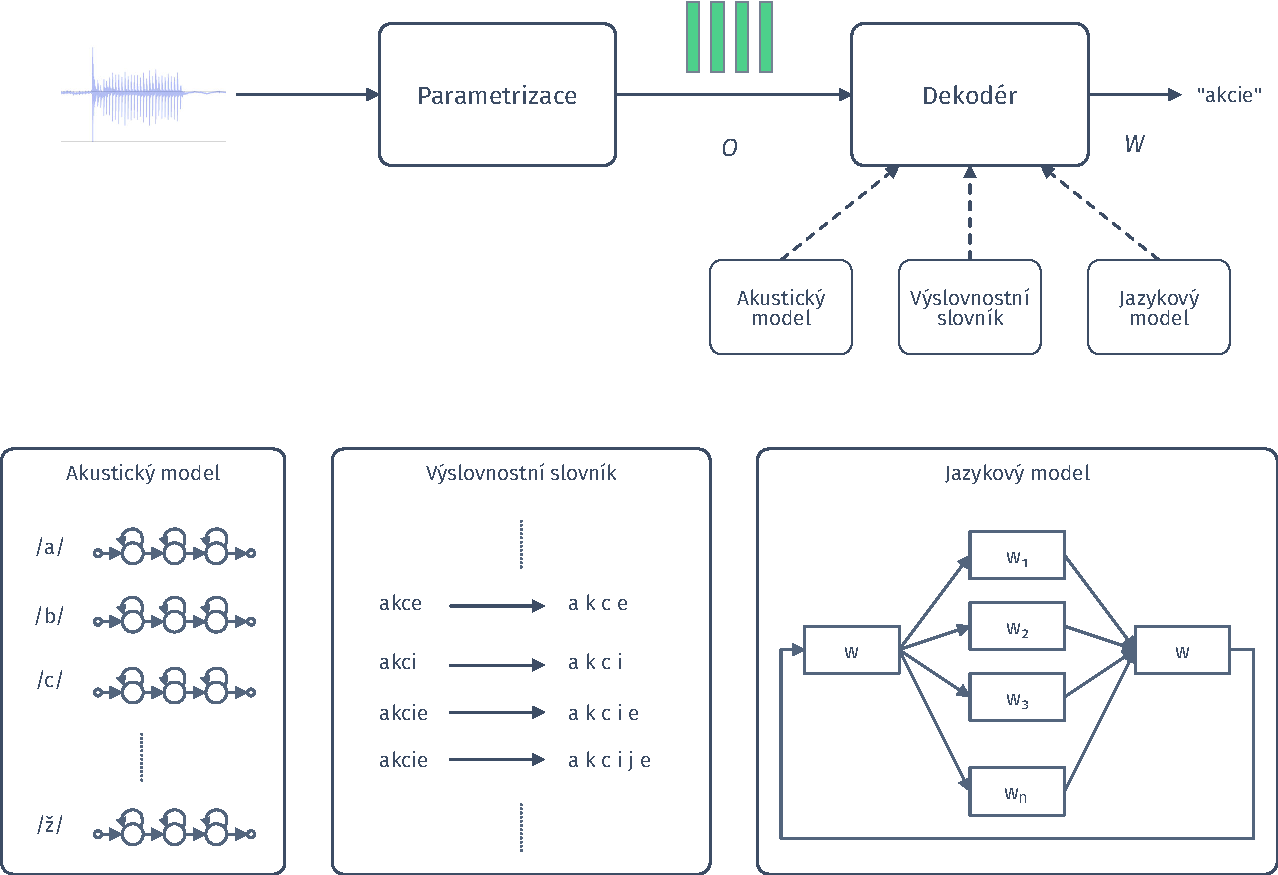
\includegraphics[width=0.9\textwidth]{./ch4-asr/img/decoding.pdf}
  \caption[Schéma ASR systému pracující se statistickou.]{Schéma automatického systému rozpoznávání řeči pracující na statistickém přístupu.}
  \label{fig:asr:decoding}
\end{figure}

\begin{equation}
  \hat{W} = \argmax_W\ P\left(W | \boldsymbol{O}\right).
  \label{eq:asr:decoding}
\end{equation}

\newpage Pomocí Bayesova pravidla je možné podmíněnou pravděpodobnost $P\left(W | \boldsymbol{O}\right)$ vyjádřit jako

\begin{equation}
  P\left(W | \boldsymbol{O}\right) = \frac{P(\boldsymbol{O}|W)P(W)}{P(\boldsymbol{O})},
\end{equation}

\noindent kde podmíněná pravděpodobnost $P(\boldsymbol{O} | W)$ odhaduje sekvenci pozorování $\boldsymbol{O}$ za předpokladu výskytu posloupnosti slov $W$. Tento výpočet je realizován \textbf{akustický modelem} (viz obr. \ref{fig:asr:decoding}). K určení $\hat{W}$ je ještě nezbytné znát pravděpodobnost výskytu požadované posloupnosti slov $P\left(W\right)$, o stanovení této pravděpodobnosti se stará \textbf{jazykový model}. Jelikož pravděpodobnost $P(\boldsymbol{O})$ je z principu nezávislá na sekvenci slov $W$, je možné rovnici (\ref{eq:asr:decoding}) upravit do tvaru

\begin{equation}
  \hat{W} = \argmax_W\ P\left(\boldsymbol{O} | W\right)P(W).
  \label{eq:asr:decoding:generic}
\end{equation}

Takto upravená rovnice představuje obecné pravidlo dekódování a její členy reprezentují základní stavební prvky ASR systému. Pro doplnění je nutné dodat, že \textbf{slovník} obsahuje seznam všech slov, se kterými je systém schopen pracovat. Tento seznam jobsahuje rovněž jejich fonetickou transkripci. Všechny tyto části jsou součástí \textbf{dekodéru}, který realizuje prohledávací strategii. V následujícím textu budou jednotlivé stavební prvky ASR systému popsány podrobněji.

% !TEX root = ../thesis.tex
\section{Parametrizace řečového signálu}
\label{chap:asr:parametrization}

Stejně jako v mnoha jiných odvětvích, i při rozpoznávání řeči je v mnoha případech inspirací člověk. Pro získání sekvence pozorování (příznaků) vycházíme z \textbf{modelování produkce řeči} a \textbf{modelování procesu slyšení}.

\subsection{Modelování produkce řeči}
\label{chap:asr:parametrization:production}

Cílem modelování produkce řeči je nalezení matematických vztahů, které poslouží k~reprezentaci fyzikálních dějů spojených s produkcí řeči. Základem je parametrizační technika \textbf{lineárního prediktivního kódování}, známá pod anglickou zkratkou LPC\footnote{Linear Predictive Coding} \cite{Benesty2007}. Vychází z představy, že hlasové ústrojí člověka je schopno vytvářet tři různé typy řečových zvuků:

\begin{itemize}
  \item \textit{samohlásky} - ty se řadí mezi znělé typy zvuků produkované periodickým buzením vznikajícím pulsy vzduchu, které jsou produkovány hlasivkami;
  \item \textit{frikativy} (např. $/f/$\footnote{Zápis $/f/$ symbolizuje foném, což je akustická reprezentace písmene, \textit{f}. Konkrétní zápisy se mohou lišit podle použité fonetické abecedy. V Čechách se nejčastěji používá abeceda $SAMPA$ či $Z\check{C}FA$.}) - někdy nazývané jako třené souhlásky, protože vznikají třením vydechovaného proudu vzduchu o překážku, kterou mouhou být například zuby nebo jazyk, v některém místě hlasového ústrojí;
  \item \textit{explozivy} (např. $/b/$, $/p/$ ap.) - také nazývané jako souhlásky výbuchové, se tvoří úplným uzavřením vydechovaného proudu vzduchu pomocí artikulačních orgánů. To se následně projeví jako krátká pauza (tzv. okluze), po které následuje náhlé jednorázové uvolnění a únik nahromaděného vzduchu (tzv. exploze) \cite{Psutka2006}.
\end{itemize}

Snahou je navrhnout takový model hlasového traktu, který bude dobře popisovat výše zmíněné řečové zvuky. Nesmí se však zapomenout na možnou přílišnou složitost~a nedostatečnou přesnost modelu. Jako ideální se může jevit lineárně časově invariantní model. Bohužel lidskou řeč lze klasifikovat jako kontinuální časově variantní a v~některých situacích dokonce nelineární proces, proto je téměř nemožné jej přesně namodelovat. Pokud však budeme předpokládat, že v konkrétním krátkém časovém úseku zůstává buzení a parametry hlasivkového traktu přibližně konstantní, tak je možné navrhnout lineární časově invariantní model řeči, který je platný pro krátké časové úseky. Tuto podmínku lze považovat za platnou pro intervaly délky od $10$ do $30\ ms$. Odtud také vychází uvažovaná perioda segmentů řeči, zmíněná v úvodu této kapitoly. Pro tyto segmenty je pak možné proces vytváření řeči modelovat pomocí tzv. \textbf{krátkodobého modelu}, který má v krátkých časových intervalech pevné parametry \cite{Holmes2001}.

Odvození obecného diskrétního modelu hlasivkového traktu je založeno na zjednodušeném modelu produkce řeči, jehož struktura je ukázána na obr. \ref{fig:asr:model:speech}. Ten je tvořen třemi dílčími částmi, konkrétně modelem hlasivek, modelem hlasivkového traktu a modelem vyzařovaného zvuku. K odvození a popisu vlastností modelu se využívá výhod Z-transformace \cite{Psutka2006}.

\begin{figure}[hbpt]
  \centering
  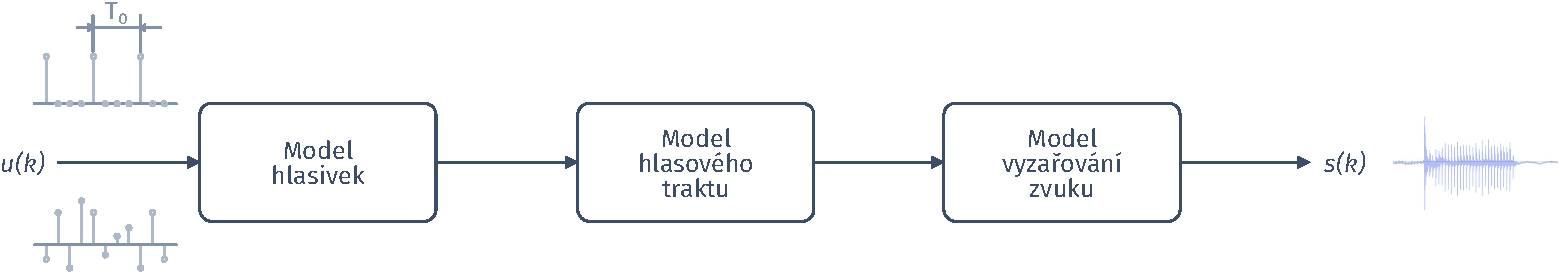
\includegraphics[width=0.9\textwidth]{./ch4-asr/img/speech_model.pdf}
  \caption{Blokové schéma modelu produkce řeči.}
  \label{fig:asr:model:speech}
\end{figure}


Krátkodobý model produkce řeči lze aproximovat celopólovým modelem charakteru filtru $H(z)$ ve tvaru

\begin{equation}
  H(z) = \frac{G}{1 + \sum_{i = 1}^{Q} a_{i} z^{-i}} = \frac{G}{A(z)},
  \label{eq:asr:lpc:generic}
\end{equation}

\noindent kde $G$ představuje celkové zesílení, $Q$ je řád modelu a $a_i$ jsou parametry modelu. Vstupem modelu je buzení $u(k)$ (viz obr. \ref{fig:asr:model:speech}), které je v případě znělých zvuků reprezentováno sledem pulsů s periodou $T_0$\footnote{Perioda základního hlasivkového tónu.} a pro neznělé zvuky je tvořeno náhodným šumem s plochým spektrem. V časové oblasti je pak diskrétní výstupní odezva při fixovaných parametrech hlasového traktu ($10 - 30\ ms$) dána konvolucí buzení a impulzní odezvy krátkodobého modelu. Na základě toho je možné model upravit do podoby znázorněné na obr. \ref{fig:asr:model:speech:excitation}, kde $u(k)$ je buzení a $s(k)$ je výstupní signál s parametry hlasového ústrojí odpovídajícími parametrům $a_i$ celopólového modelu.

\begin{figure}[hbpt]
  \centering
  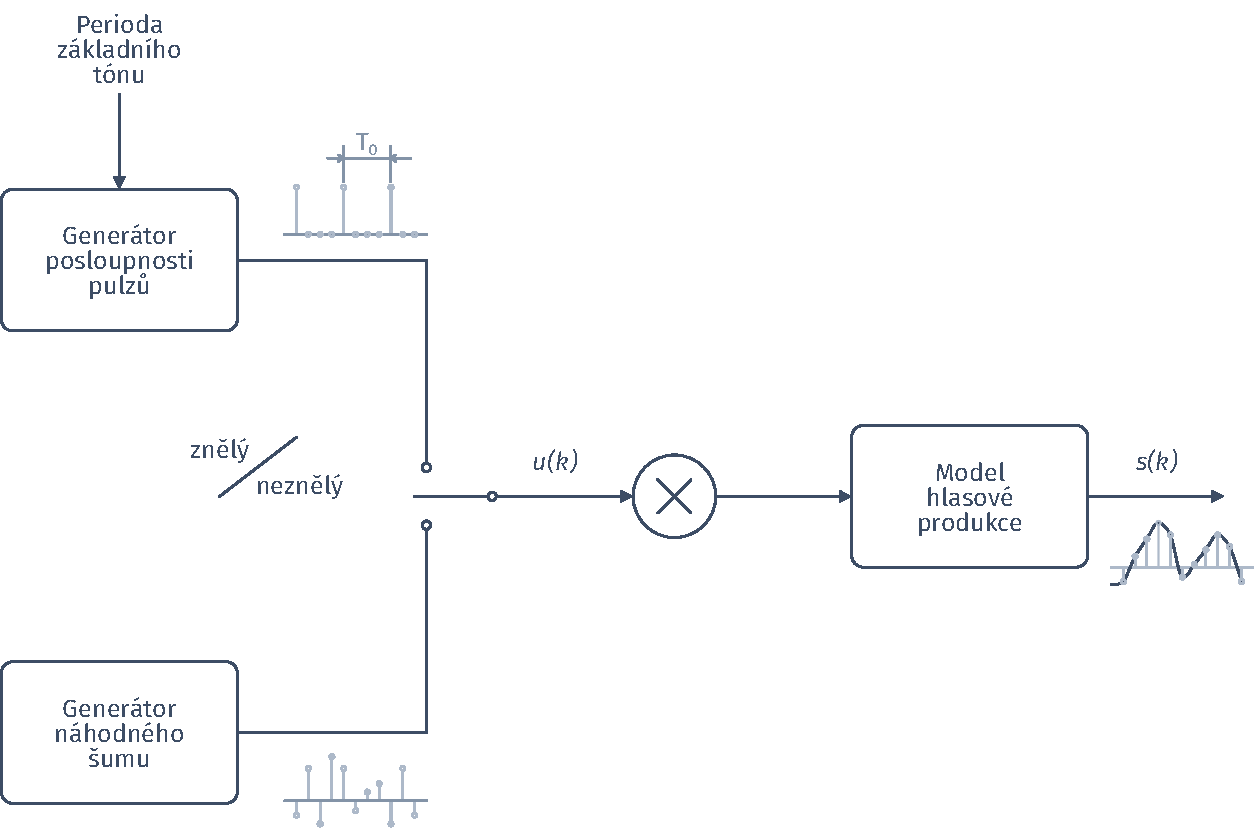
\includegraphics[width=0.9\textwidth]{./ch4-asr/img/speech_process.pdf}
  \caption{Blokové schéma upraveného modelu produkce řeči.}
  \label{fig:asr:model:speech:excitation}
\end{figure}

K odhadu parametrů $a_i$ slouží \textbf{lineární prediktivní analýza}. Odhad probíhá přímo z krátkodobého řečového signálu. Přenosové vlastnosti krátkodobého modelu je možné popsat rovnicí (\ref{eq:asr:lpc:generic}). Myšlenka metody LPC vychází z předpokladu, že vzorek $k$ řečového signálu je možné popsat lineární kombinací $Q$ předchozích vzorků a buzení $u(k)$, což lze matematicky vyjádřit pomocí následující rovnice ve tvaru

\begin{equation}
  s(k) = - \sum_{i = 1}^{Q} a_i s(k-1) + Gu(k).
  \label{eq:asr:lpc:generic:edited}
\end{equation}

\noindent %Z rovnice (\ref{eq:asr:lpc:generic:edited}) 
Je patrné, že se LPC snaží odhadnout parametry modelu $a_i$ a zesílení $G$ pomocí známé reálně naměřené posloupnosti vzorků řeči $s(k)$. K odhadu se používá principu minimalizace kvadratické chyby krátkodobé energie signálu $e\left(k\right)$. Ta je v časové oblasti popsána vztahem

\begin{equation}
  E = \sum_{k} e^2(k) = \sum_{k} \left[ s(k) - s'(k)\right]^2 = \sum_{k} \left( s(k) + \sum_{i = 1}^{Q} a_i s(k-1) + Gu(k) \right),
\end{equation}

\noindent kde $s(k)$ jsou vzorky reálného řečového signálu a $s'(k)$ jsou ty predikované LPC filtrem. Pro nalezení minimální hodnoty krátkodobé chyby predikce $E$ pro konkrétní analyzovaný segment, je použita metoda nejmenších čtverců. K výpočtu konkrétních koeficientů modelu $a_i$ je možné použít rekurzivního Durbinova algoritmu \cite{Holmes2001}.

Další možností jak modelovat hlasový trakt je využít popis pomocí \textbf{kepstrálních koeficientů lineární predikce} $c\left(k\right)$. Kepstrum k-tého mikrosegmentu řečového signálu $s\left(k\right)$ je definováno vztahem % (\ref{eq:asr:lpc:cepstrum:generic}), 


\begin{equation}
  c(k) = \mathcal{F}^{-1}\left\{\log\left| \mathcal{F}\left\{s(k)\right\} \right|\right\}.
  \label{eq:asr:lpc:cepstrum:generic}
\end{equation}

\noindent kde $\mathcal{F}$ představuje operátor diskrétní Fourierovy transformace (DFT) a $\mathcal{F}^{-1}$ reprezentuje inverzní diskrétní Fourierovy transformace (IDFT). Postup výpočtu je znázorněn na obr. \ref{fig:asr:model:speech:cepstrum}.

\begin{figure}[hbpt]
  \centering
  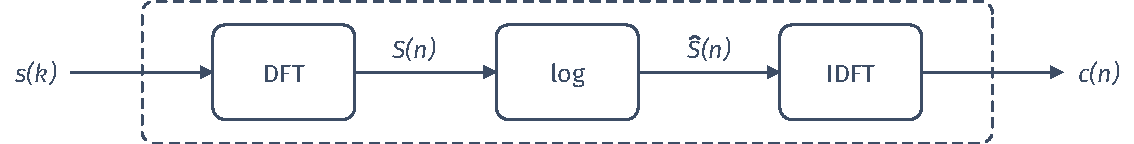
\includegraphics[width=0.9\textwidth]{./ch4-asr/img/cepstrum.pdf}
  \caption{Blokové schéma principu výpočtu kepstra.}
  \label{fig:asr:model:speech:cepstrum}
\end{figure}

Pro získání kepstrálních koeficientů lineární predikce lze využít vztah (\ref{eq:asr:lpc:generic}), který po zlogaritmování přejde do tvaru

\begin{equation}
  \log H(z) = \log \left( \frac{G}{A(z)} \right).
  \label{eq:asr:lpc:cepstrum}
\end{equation}

\noindent Člen $A(z)$ je polynomem proměnné $z^{-1}$ řádu $Q$. Pokud všechny jeho kořeny leží uvnitř jednotkové kružnice, tak lze aplikovat Taylorův rozvoj a vztah (\ref{eq:asr:lpc:cepstrum}), tedy lze zapsat jako

\begin{equation}
  \log \left( \frac{G}{A(z)} \right) = c(0) + c(1)z^{-1} + \dots = \sum_{k=0}^{\infty} c(k)z^{-k},
  \label{eq:asr:lpc:cepstrum:taylor}
\end{equation}

\noindent kde $c(k)$ jsou tzv. kepstrální koeficienty LPC. Po zderivování obou stran rovnice přejde vztah (\ref{eq:asr:lpc:cepstrum:taylor}) do tvaru

\begin{equation}
  - \sum_{i=1}^{Q} ia_iz^{-i} = \left( \sum_{k=0}^{\infty} kc(k)z^{-k} \right)\left( \sum_{i=0}^{Q} a_iz^{-i}\right).
  \label{eq:asr:lpc:cepstrum:deriv}
\end{equation}

\noindent Jestliže se $a_i = 1$, pak lze po roznásobení pravé strany rovnice (\ref{eq:asr:lpc:cepstrum:deriv}) a po následném porovnání členů u stejných mocnin proměnné $z$ zapsat vztahy pro výpočet kepstrálních koeficientů LPC ve tvaru

\begin{align}
  \begin{split}
    c(1) &= -a_1, \\
    c(k) &=
    \begin{cases}
      - a_k - \sum_{i=1}^{k-1} \left(\frac{i}{k}\right) c(i) a_{k-1},  & \quad \text{pro } 2 \leq k \leq Q, \\
      - \sum_{i=1}^{Q} \left(\frac{k - i}{k}\right) c(k-i) a_i,  & \quad \text{pro } k = Q + 1, Q + 2, \dots \quad ,
    \end{cases}
  \end{split}
  \label{eq:asr:lpc:cepstrum:coef}
\end{align}

\noindent kde $k = 1, 2, \dots , Q^{*}$. $Q^{*}$ je počet kepstrálních koeficientů pro které musí platit $Q^{*} \geq Q$. Kepstrální koeficienty LPC jsou vztaženy ke spektrální obálce mikrosegmentu řeči odvozené LPC analýzou. 

Spektrální obálku je následně možné získat z rovnice (\ref{eq:asr:lpc:generic}) dosazením $z = e^{j\omega}$. Pro uspokojivou reprezentaci se tradičně volí $Q$ v rozmezí $7-15$ v závislosti na spektrální šířce přenášeného pásma a požadované přesnosti aproximace. Z toho plyne, že pro popis mikrosegmentu řeči by mohl být dostačující příznakový vektor o $15$ koeficientech.

\subsection{Modelování procesu slyšení}
\label{chap:asr:parametrization:hearing}

Zvuk představuje mechanické vlnění hmotných částic, které se šíří v plynném, kapaném nebo tuhém prostředí. Z fyziologického pohledu je však zvuk považován pouze za slyšitelné vlnění. To je takové, které je schopno vnímat sluchové ústrojí člověka. Zpravidla se jedná o frekvence $16\ Hz - 20\ kHz$. Pro každého člověka je ale toto rozmezí individuální a mění se s věkem. S přibývajícím věkem a sluchovou zátěží klesá hlavně horní mezní kmitočet \cite{Psutka2006}.

To, zda je člověk schopen daný zvuk slyšet, však není závislé pouze na frekvenci zvuku. Velmi podstatná je i intenzita zvuku, která se rovná energii zvukového vlnění, která projde za jednotku času jednotkovou plochou kolmou ke směru šíření vln. Zároveň je úměrná akustickému tlaku zvukové vlny, tj. tlaku, kterým zvukové vlny působí na nějakou překážku. V případě člověka lze překážkou chápat ušní bubínek. Závislost mezi intenzitou zvuku $I\ \left[Wm^{-2}\right]$ a akustickým tlakem $p\ \left[Pa\right]$ je vyjádřen vztahem

\begin{equation}
  I = \frac{p^{2}}{z},
  \label{eq:asr:mfcc:intesity}
\end{equation}

\noindent kde $z$ je měrná akustická impedance prostředí, kterým se zvuk šíří. Lidské ucho je schopno vnímat akustický tlak v rozsahu od $2\cdot10^{-5}$ až $2\cdot10^{2}\ Pa$, tj. v rozsahu sedmi řádů. Z praktického důvodu se tedy používá logaritmické stupnice. K vyjadřování pak slouží logaritmus poměru uvažované veličiny a mezinárodně normované referenční hodnoty téže veličiny \cite{Psutka2006}. Hladina intenzity $L_{I}$ je pak definována vztahem

\begin{equation}
  L_{I} = 10\log_{10}\frac{I}{I_{0}},
  \label{eq:asr:mfcc:intesity:level}
\end{equation}

\noindent kde $I$ představuje intenzitu zvuku a $I_{0} = 10^{-12}\ Wm^{-2}$ referenční hodnotu intenzity. Pro hladinu akustického tlaku platí

\begin{equation}
  L_{p} = 20\log_{10}\frac{p}{p_{0}},
  \label{eq:asr:mfcc:pressure:level}
\end{equation}

\noindent kde $p$ je akustický tlak a $p_{0} = 2\cdot10^{-5}\ Pa$ je referenční hodnota akustického tlaku. Hodnoty veličin $L_{I}$ a $L_{p}$ jsou obvykle udávány v decibelech. %$\left[dB\right]$.

Důležitým pojmem je pak \textbf{práh slyšitelnosti}, který představuje minimální intenzitu zvuku potřebnou k tomu, aby jej šlověk mohl slyšet, viz obr. \ref{fig:asr:mfcc:acoustic:characteristic}. Tento práh je zcela subjektivní a je závislý na frekvenci. Obecně je lidský sluch nejcitlivější na frekvence $3 - 4\ kHz$. Směrem k nižším i vyšším kmitočtům citlivost sluchu klesá. \textbf{Práh bolesti} představuje horní mez intenzity sluchového pole (viz obr. \ref{fig:asr:mfcc:acoustic:characteristic}), při níž již posluchač pociťuje bolest. Překročení této meze může vést k poškození sluchu \cite{Holmes2001}.

\begin{figure}[hbpt]
  \centering
  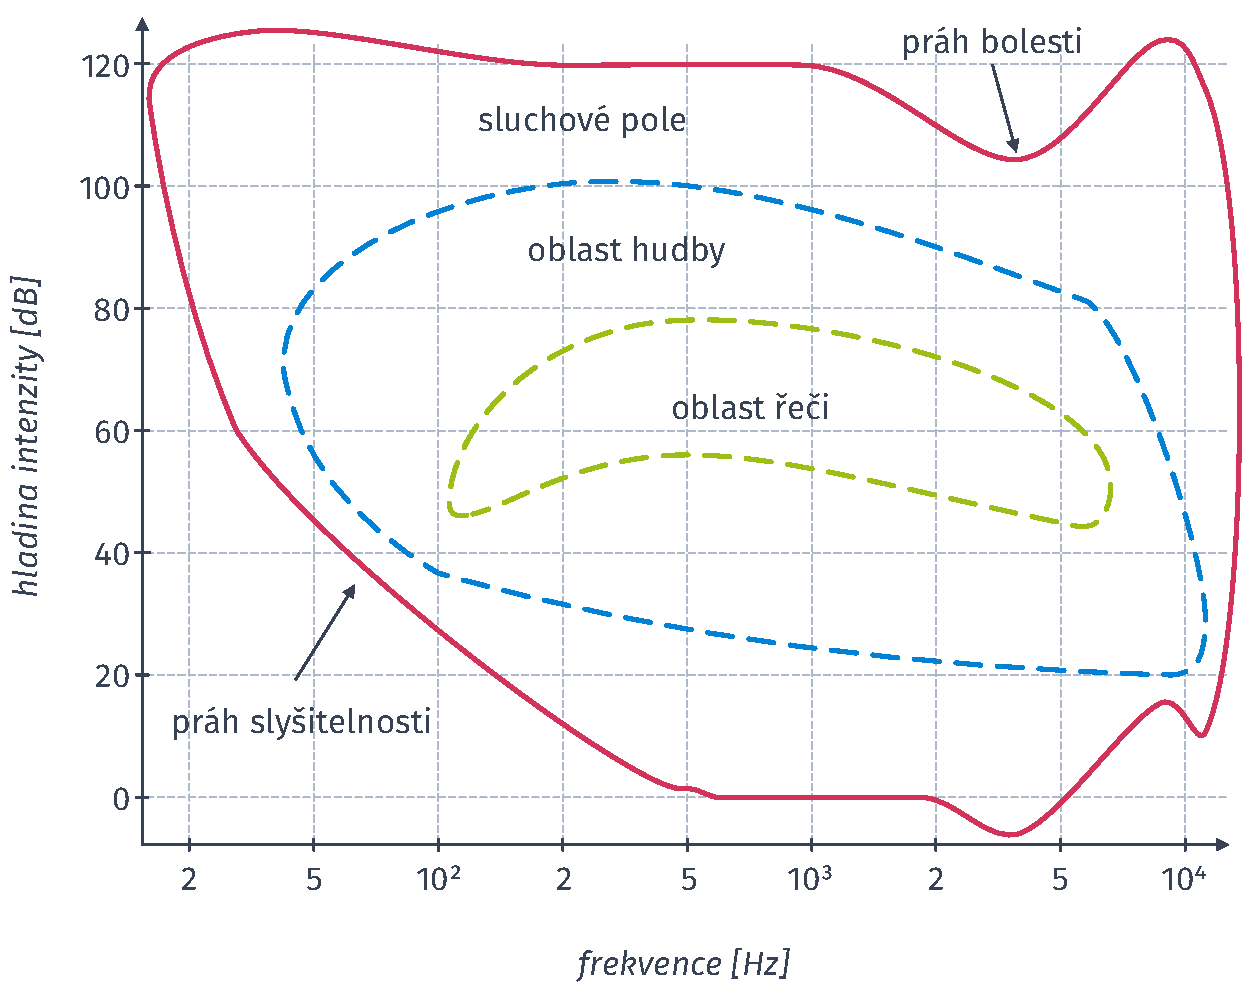
\includegraphics[width=0.75\textwidth]{./ch4-asr/img/listening_perception.pdf}
  \caption[Charakteristické oblasti vnímání akustického signálu.]{Charakteristické oblasti vnímání akustického signálu lidským sluchem. $L_p = 20log(p/p0),\ p0 = 2\bullet10^{–5}\ Pa$.}
  \label{fig:asr:mfcc:acoustic:characteristic}
\end{figure}

Hlasitost zvuku je závislost intenzity na frekvenci a je zcela subjektivní pocit, kterým člověk posuzuje intenzitu daného zvuku. Na obr. \ref{fig:asr:mfcc:acoustic:levels} jsou vyznačeny hladiny hlasitosti, které vznikly spojením bodů ve sluchovém poli (obr. \ref{fig:asr:mfcc:acoustic:characteristic}), odpovídající tónům, které člověk vnímá stejně hlasitě. Z křivek je patrné, že subjektivní hlasitost se mění s frekvencí zvuku. Zvuky s nižší frekvencí vnímáme méně hlasitěji než zvuky s vyšší frekvencí, zejména pak zvuky v rozmezí $3 - 4\ kHz$ \cite{Psutka2006}.

\begin{figure}[hbpt]
  \centering
  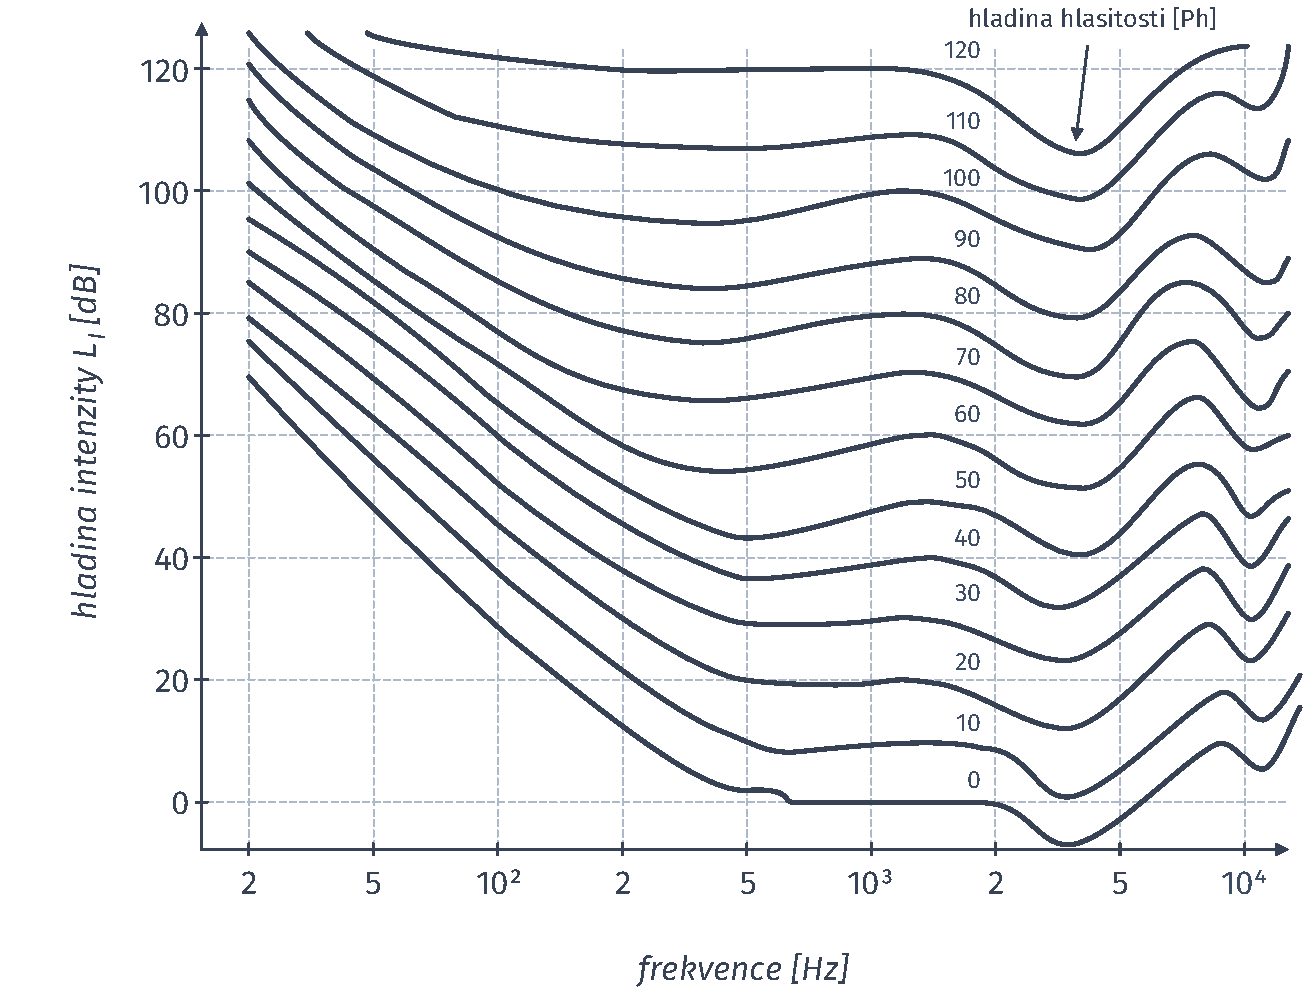
\includegraphics[width=0.75\textwidth]{./ch4-asr/img/listening_levels.pdf}
  \caption[Křívky stejné hlasitosti.]{Křivky stejné hlasitosti. $L_p = 20log(p/p0),\ p0 = 2\bullet10^{–5}\ Pa$.}
  \label{fig:asr:mfcc:acoustic:levels}
\end{figure}

Principem modelování procesu slyšení je postižení kompenzace nelineárního vnímání frekvencí lidským sluchem a respektování maskování zvuků včetně tzv. kritických pásem slyšení. Maskování zvuků je přirozená vlastnost lidského sluchu. Rozumí se jím jev, kdy je vnímání jednoho zvuku ovlivněno přítomností jiného zvuku. Jinými slovy lze říci, že přítomnost jednoho zvuku zvyšuje práh slyšitelnosti pro jiný zvuk. Ten buď zní současně nebo s drobným časovým odstupem od toho prvního. Tento jev je jakýsi \uv{psychologický filtr}, který ignoruje veškerý šum ležící mimo určité kritické pásmo slyšení. Šířka kritického pásma je přitom závislá na frekvenci poslouchaného tónu. Často užívanými metodami pro modelování procesu slyšení jsou \textbf{melovská kepstrální filtrace} a \textbf{perceptivní lineární prediktivní analýza}.

\subsubsection{Melovské kepstrální koeficienty}

Metoda melovských frekvenčních kepstrálních koeficientů (MFCC) se snaží respektovat výše zmíněné vlastnosti lidského sluchu, především se snaží dodržet kritická pásma slyšení a vliv subjektivního vnímání výšky tónů.

Základem MFCC je využití banky filtrů a lineárního rozložení frekvencí v tzv. \textbf{melovské frekvenční škále} definované vztahem

\begin{equation}
  f_m = 2595 \log \left(1 + \frac{f}{700}\right),
  \label{eq:asr:mfcc:melscale}
\end{equation}

\noindent kde $f \left[Hz\right]$ je frekvence v lineární škále a $f_m \left[mel\right]$ je odpovídající frekvence v melovské stupnici. Melovský filtr má trojúhelníkový tvar. Banka obsahuje $M^{*}$ filtrů rozmístěných lineárně v melovských frekvenčních souřadnicích, a to tak, že dva sousední filtry se navzájem o polovinu překrývají. Pro střední frekvence jednotlivých filtrů $b_{m,i}$ v melovské škále platí vztah

\begin{equation}
  b_{m,i} = b_{m,i-1} + \Delta_{m},
  \label{eq:asr:mfcc:freq}
\end{equation}

\noindent kde $b_{m, 0} = 0\ mel$, $i = 1, 2,\ \dots\ , M^{*}$, a $\Delta_m = B_{m,w} / (M^{*} + 1)$, kde $B_{m,w}$ je celková šířka pásma v melovské škále. Ukázka banky filtrů v této škále je znázorněna na obr. \ref{fig:asr:mfcc:bank:mel}. Pro výpočet odezvy filtrů je však nezbytné přepočítat všechny koeficienty FFT do melovské frekvenční škály.

\begin{figure}[hbpt]
  \centering
  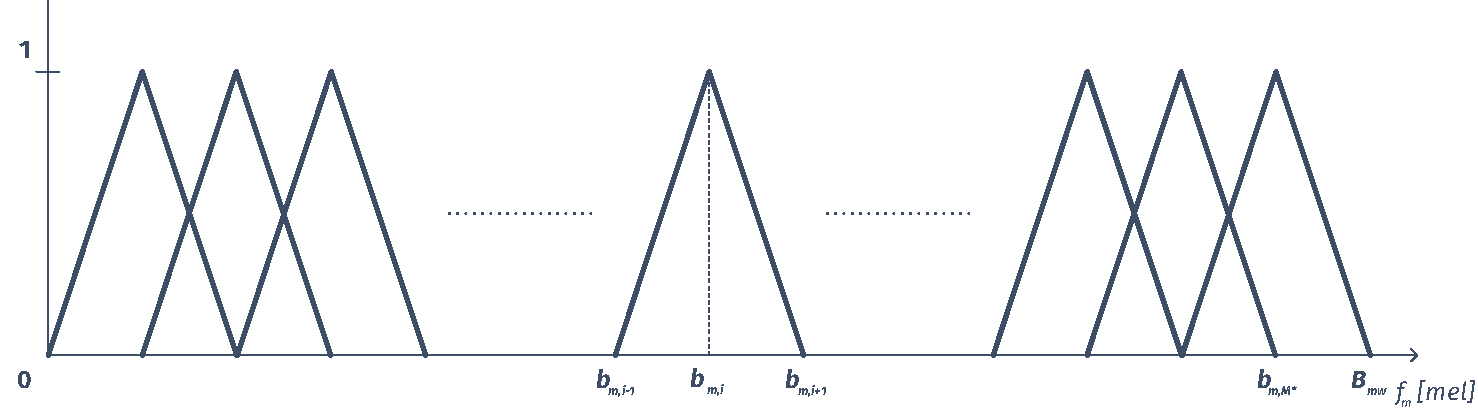
\includegraphics[width=0.9\textwidth]{./ch4-asr/img/filter_bank-mel.pdf}
  \caption{Rozložení banky trojúhelníkových filtrů v melovské frekvenční škále.}
  \label{fig:asr:mfcc:bank:mel}
\end{figure}

\noindent Vhodnější je vyjádření trojúhelníkových filtrů ve frekvenční škále s měřítkem v herzích. K přepočtu středních frekvencí $b_{m,i}$ se využívá inverzního vztahu k (\ref{eq:asr:mfcc:melscale}), tedy

\begin{equation}
  f = 700 \left[ \exp\left( 0,887.10^{-3} f_m \right) - 1 \right].
  \label{eq:asr:mfcc:melscale:inverse}
\end{equation}

\noindent Střední frekvence $b_i$ jednotlivých filtrů jsou vyjádřené také v herzích. Na rozdíl od popisu v melovské škále jsou filtry rozmístěny nelineárně napříč celým analyzovaným spektrem, viz obr. \ref{fig:asr:mfcc:bank:hz}.

\begin{figure}[hbpt]
  \centering
  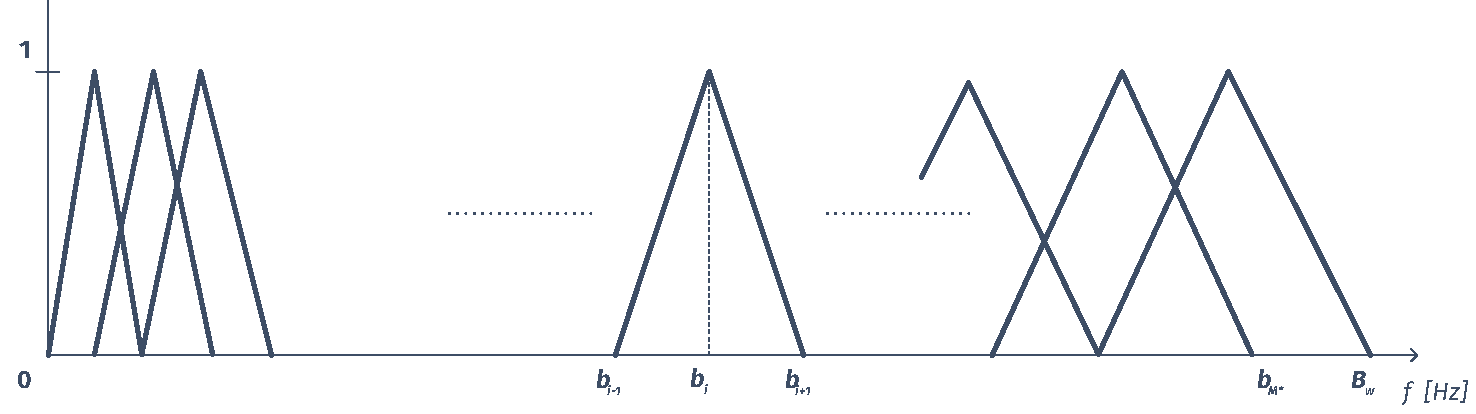
\includegraphics[width=0.9\textwidth]{./ch4-asr/img/filter_bank-hz.pdf}
  \caption{Rozložení banky trojúhelníkových filtrů ve frekvenční škále.}
  \label{fig:asr:mfcc:bank:hz}
\end{figure}

Na vstup systému jsou postupně přivedeny mikrosegmenty řečového signálu\footnote{Jednotlivé mikrosegmenty byly nejprve předzpracovány , tj. prošly tzv. preemfází. Ta spočívá ve zdůraznění amplitud spektrálních složek řečového signálu s jejich vzrůstající frekvencí \cite{Psutka2006}.} $s\left(k\right)$ o konstantní délce a pro ně jsou určeny odpovídající koeficienty $c\left(k\right)$. Pro jednotlivé mikrosegmenty je pomocí FFT vypočteno amplitudové spektrum $\left| S(f) \right|$ a následuje klíčová část celého procesu, melovská filtrace. Odezvy filtrů ve frekvenční oblasti lze stanovit pomocí vztahu

\begin{equation}
  y_m(i) = \sum_{f=b_{i-1}}^{b_{i+1}} \left| S(f) \right| u\left(f, i\right),  \quad i = 1, 2,\ \dots\ ,M^{*},
  \label{eq:asr:mfcc:freq:responce}
\end{equation}

\noindent kde frekvence $f$ jsou vybírány ze souboru frekvencí využívaných při FFT výpočtu a $u(f, i)$ je vyjádření konkrétního trojúhelníkového filtru $i$. Průchod filtrem tedy znamená, že každý koeficient FFT je násoben odpovídajícím ziskem filtru a výsledky jsou pro příslušné filtry akumulovány. Logaritmováním akumulovaných koeficientů $y_{m}(i)$ je realizován převod do kepstrální oblasti. Tento krok příznivě omezí dynamiku signálu \cite{Benesty2007}. Posledním krokem při výpočtu melovských kepstrálních koeficientů $\left\{c_m\left(j\right)\right\}_{j=1}^{M}$ je provedení IDFT podle vztahu (\ref{eq:asr:lpc:cepstrum:generic}). V případě MFCC se ale používá diskrétní kosinová transformace (DCT), protože spektrum je reálné a symetrické. K výpočtu slouží vztah

\begin{equation}
  c_{m}(j) = \sum_{i=1}^{M^{*}} \log y_m(i) \cos\left( \frac{\pi j}{M^{*}}\left(i - 0,5\right) \right) \quad \text{pro}\ j = 0, 1,\ \dots\ ,M,
  \label{eq:asr:mfcc:coef}
\end{equation}

\noindent kde $M^{*}$ je počet pásem melovkého pásmového filtru a $M$ je počet melovských kepstrálních koeficientů. Počet těchto koeficientů $M$ se volí podstatně menší než je počet pásem melovského pásmového filtru $M^{*}$, obvykle se uvažuje prvních $10\ \text{až}\ 13$ koeficientů. Velmi často se také používá $1.$ a $2.$ z těchto koeficientů, protože svým způsobem zohledňují dynamickou složku řeči.

\subsubsection{Perceptivní lineární prediktivní analýza}

Stejně jako MFCC, tak také i \textbf{perceptivní lineární prediktivní analýza (PLP)} vychází z lidského vnímání a slyšení zvuků. Snaha je postihnout z psychofyziky slyšení zejména kritická pásma spektrální citlivosti, vztah mezi intenzitou a vnímáním hlasitosti a také křivky stejné hlasitosti \cite{Psutka2006}. PLP podobně jako LPC pak aproximuje získané sluchové spektrum koeficienty autoregresního celopólového modelu.

Prvním krokem PLP analýzy je \textbf{výpočet výkonového spektra řečového signálu}. Pro konkrétní předzpracovaný\footnote{Ještě před výpočtem je stejně jako u MFCC aplikována preemfáze.} mikrosegment řečového signálu $s(k)$ aplikujeme DFT. Krátkodobé spektrum je pak definováno vztahem

\begin{equation}
  P\left(\omega\right) = \left| S\left(\omega\right) \right|^{2} = \left[Re\ S\left(\omega\right)\right]^2 + \left[Im\ S\left( \omega \right) \right]^2.
  \label{eq:asr:plp:spectr}
\end{equation}

\noindent Poté následuje kompenzace nelineárního vnímání změn ve výšce zvuku. Vnímání je logaritmické, proto je nutné provést nelineární transformaci frekvenční osy pomocí vzorce

\begin{equation}
  \Omega\left(\omega\right) = 6 \ln \left( \frac{\omega}{1200\pi} + \sqrt{\left(\frac{\omega}{1200\pi}\right)^2 + 1} \right),
  \label{eq:asr:plp:transform}
\end{equation}

\noindent kde $\omega = 2\pi f\ \left[rad/s\right]$ a $\Omega\left(\omega\right)\ \left[Bark\right]$.

Zahrnutí kritických pásem slyšení (tzv. maskování zvuku) je realizováno navržením vhodného filtru typu pásmová propust šířky jednoho kritického pásma. Stejně jako v případě MFCC se jedná o banku filtrů, kde na sebe jednotlivé filtry ve frekvenční oblasti navazují.
%Na Barkově frekvenční ose (viz (\ref{eq:asr:plp:transform})) mají všechny filtry šířku $1$ a jsou lineárně rozmístěny.
Na obr. \ref{fig:asr:plp:filter} je zobrazen průběh jednoho takového filtru. Filtr má strmost $+20\ dB/Bark$ směrem k nižším frekvencím a $-50\ dB/Bark$ směrem k vyšším frekvencím.

\begin{figure}[hbpt]
  \centering
  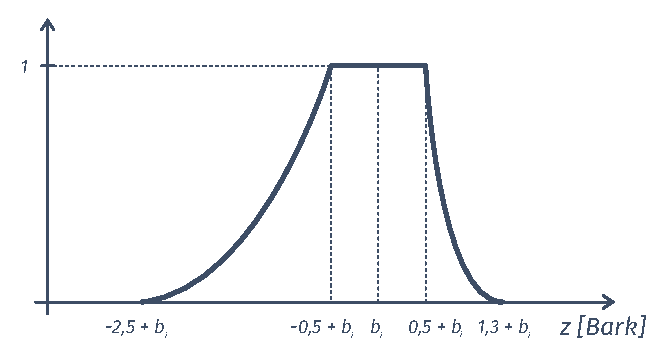
\includegraphics[width=0.5\textwidth]{./ch4-asr/img/plp_filter.pdf}
  \caption{Ukázka filtru umístěného na Barkově frekvenční ose.}
  \label{fig:asr:plp:filter}
\end{figure}

\newpage \noindent Na Barkově frekvenční ose mají jednotlivé filtry šířku $1$ a jsou podél ní lineárně rozmístěny viz obr. \ref{fig:asr:plp:bank},
% Rozmístění filtrů na Barkově frekvenční ose je pak znázorněno na obr. \ref{fig:asr:plp:bank}.

\begin{figure}[hbpt]
  \centering
  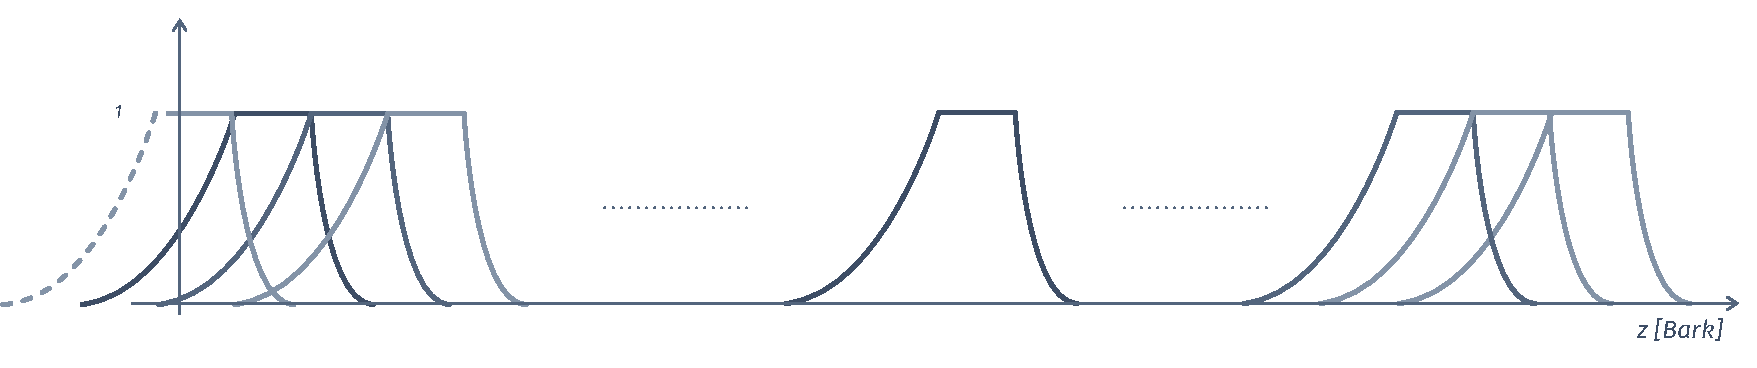
\includegraphics[width=0.9\textwidth]{./ch4-asr/img/plp-bank.pdf}
  \caption{Rozmístění filtrů na Barkově frekvenční ose.}
  \label{fig:asr:plp:bank}
\end{figure}

Jelikož člověk vnímá intenzitu zvuku v závislosti na frekvenci, tak je potřeba provést \textbf{přizpůsobení křivkám stejné hlasitosti}. Na začátku je důležité definovat referenční hlasitost, tj. hlasitost, na kterou bude normalizována. Obvykle se volí $40\ Ph$ \cite{Psutka2006}, což přibližně odpovídá hlasitosti běžné řeči. K normalizaci je použit inverzní filtr popsaný vztahem

\begin{equation}
  E\left(\omega\right) = K \frac{\omega^4\left(\omega^2 + 56,9 \cdot 10^6\right)}{\left(\omega^2 + 6,3 \cdot 10^6\right)^2\left(\omega^2 + 379,4 \cdot 10^6\right)\left(\omega^6 + 9,6 \cdot 10^{26}\right)},
  \label{eq:asr:plp:filter}
\end{equation}

\noindent kde $\omega = 2\pi f$ a $K$ je konstanta nastavená podle požadovaného zesílení. Přizpůsobení křivce stejné hlasitosti je pak možné například přenásobením celého výkonového spektra mikrosegmentů podle vztahu

\begin{equation}
  P'\left(\omega\right) = E\left(\omega\right)P\left(\omega\right),
  \label{eq:asr:plp:filter:application1}
\end{equation}

\noindent kde $P'\left(\omega\right)$ je spektrum transformované na stejnou hlasitost. Případně lze upravit tvar jednotlivých filtrů pomocí vztahu

\begin{equation}
  \Phi\left(\omega, i\right) = E\left(\omega\right)\Psi\left(\omega - \omega_i, i\right),
  \label{eq:asr:plp:filter:application2}
\end{equation}

\noindent kde $\Phi\left(\omega, i\right)$ je nový tvar filtru $i$ v závislosti na frekvenci $\omega$, $\Psi\left(\omega - \omega_i, i\right)$ je odezva filtru $i$ se středovou frekvencí $\omega_i$.

Po přizpůsobení následuje \textbf{výpočet energie jednotlivých filtrů}, to je obdobné jako u MFCC. Výpočet se provádí pro jednotlivé filtry a výsledky se pak sčítají. Matematicky to je zapsáno vztahem

\begin{equation}
  \zeta_m = \sum_{\Omega = \Omega_m - 2,5}^{\Omega_m + 1,3} P\left(\Omega\right)\Phi\left(\Omega, m\right), \quad\ m=1, 2,\ \dots\ M - 2,
  \label{eq:asr:plp:energy}
\end{equation}

\noindent kde $M$ je počet použitých filtrů (kritických pásem).

Dalším krokem výpočtu je uplatnění \textbf{\uv{zákona slyšení}}. Ten popisuje závislost mezi intenzitou a vnímanou hlasitostí. Na energie $\zeta_m$ je aplikována nelineární transformace vyjádřena vztahem

\begin{equation}
  \xi_m = \left(\zeta_m\right)^{0,3}, \quad\ m = 1, 2,\ \dots\ M-2,
  \label{eq:asr:plp:energy:transform}
\end{equation}

\noindent kde $M$ je opět počet filtrů. Díky této operaci dojde také k redukci proměnlivosti \uv{výstupů} kritických pásmových filtrů a výsledný hledaný celopólový model může být relativně nízkého řádu.

Finálním krokem je \textbf{aproximace celopólového modelu}. Ta vychází z výpočtu koeficientů celopólového modelu metody LPC, kde je model popsán vztahem (\ref{eq:asr:lpc:generic:edited}). Pro chybu predikce pak platí

\begin{equation}
  e\left(k\right) = \sum_{k} \left(s\left(k\right) + \sum_{i=1}^{Q} a_i s\left(k - i\right)\right).
  \label{eq:asr:plp:error}
\end{equation}

\noindent Aplikací Z-transformace a uvážením rovnice (\ref{eq:asr:lpc:generic}), je možné vztah (\ref{eq:asr:plp:error}) upravit do tvaru

\begin{equation}
  E\left(z\right) = \left[1 + \sum_{i=1}^{Q} a_i z^{-i}\right] S\left(z\right) = A\left(z\right)S\left(z\right),
  \label{eq:asr:plp:error:transform}
\end{equation}

\noindent kde $A\left(z\right)$ je inverzní filtr a $E\left(z\right)$, resp. $S\left(z\right)$ jsou získané Z-transformací $e\left(k\right)$, resp. $s\left(k\right)$. Celkovou chybu predikce je pak možné vyjádřit vztahem

\begin{equation}
  E\left(z\right) = \frac{1}{2\pi} \int_{-\pi}^{\pi} P\left(\omega\right) A\left(e^{j\omega}\right) A\left(e^{-j\omega}\right)d\omega,
  \label{eq:asr:plp:error:final}
\end{equation}

\noindent kde $P\left(\omega\right)$ je vypočtené výkonové spektrum. Podobně jako u LPC hledané řešení odpovídá hodnotám, pro něž je celková chyba autokorelační funkce $R\left(i\right)$ minimální. Pro konečný počet známých frekvencí je tato funkce definována vztahem

\begin{equation}
  R\left(i\right) = \frac{1}{N} \sum_{n=0}^{N-1} P\left(\omega_n\right) \cos\left(i\omega_n\right),
  \label{eq:asr:plp:error:solution}
\end{equation}

\noindent kde $i = 0,\ \dots\ Q$, $Q$ je řád autoregresního modelu a $N$ je počet bodů spektrální charakteristiky. Frekvence $\omega_n$ jsou ty, pro které jsou známé spektrální hodnoty. Pro dobrou aproximaci se volí $Q = 5$ \cite{Benesty2007}. \textbf{Výpočet kepstrálních koeficientů PLP} lze pak pro známé hodnoty $R\left(i\right)$, podobně jako u LPC, určit Durbinovým algoritmem. Nalezené koeficienty lze využít jako příznaky při návrhu parametrizátoru řeči
\cite{Holmes2001}.

K vytvoření parametrizátoru je možné použít libovolnou výše popsanou metodu. %metodu představenou v \ref{chap:asr:parametrization:production} a \ref{chap:asr:parametrization:hearing}. 
V současnosti ale převládají metody postavené na principu fungování lidského sluchu, protože amplifikují podstatnou informaci zakódovanou v řeči.

% !TEX root = ../thesis.tex
\section{Akustické modelování}
\label{chap:asr:acoustic}

Akustický model představuje v rovnici (\ref{eq:asr:decoding:generic}) podmíněnou pravděpodobnost $p(O|W)$. Úkolem akustického modelu je poskytnout co nejpřesnější odhad této pravděpodobnosti pro libovolnou posloupnost vektorů příznaků $O = \left\{o_1 o_2\ \dots\ o_T\right\}$. Velmi vhodným způsobem modelování řeči se ukázalo být využití tzv. \textbf{skrytých Markovových modelů (HMM)}. Ty vycházejí z principu vytváření řeči člověkem. V průběhu produkce řeči se hlasové ústrojí nachází vždy v krátkém časovém úseku nachází v jednom z konečného počtu konfiguracé. V tomto mikrosegmentu je pak hlasovým ústrojím generovám krátký signál, který zavisí na aktuální konfiguraci. Tento vyprodukovaný zvuk je metodami (popsanými v \ref{chap:asr:parametrization}) převeden na vektor příznaků $O$.

Skrytý Markovův model je model stochastického procesu. Na ten je možné nahlížet jako na pravděpodobnostní konečný automat, který v diskrétních časových okamžicích generuje náhodnou posloupnost vektorů příznaků $O = \left\{o_1 o_2\ \dots\ o_T\right\}$. Model v každém časovém kroku změní stav svůj $s_j$ podle předem daných pravděpodobností přechodu $a_{ij}$. Přechod ze stavu $s_i$ do stavu $s_j$ má za následek vygenerování výstupního vektoru pozorování $o_t$ a to podle rozdělení výstpní pravděpodobnosti $b_j\left(o_t\right)$ příslušné k tomuto stavu \cite{Psutka2006}.

Podmínění pravděpodobnost přechodu $a_{ij}$ určuje, s jakou pravděpodobností přechází model ze stavu $i$ v čase $t$, do stavu $j$ v čase $t+1$. Platí tedy

\begin{equation}
  a_{ij} = p\left(s\left(t+1\right)=s_j|s\left(t\right)=s_i\right),
  \label{eq:asr:acoustic:conditional}
\end{equation}

\noindent kde $s\left(t\right)$ je stav modelu v čase $t$. Další podmínkou je, že pro všechny stavy $i$, $i=1,2,\dots\,N$, platí

\begin{equation}
  \sum_{j=1}^{N} a_{ij} = 1.
  \label{eq:asr:acoustic:state:condition}
\end{equation}

\noindent Funkce rozdělení výstupní pravděpodobnosti $b_j\left(o_t\right)$ popisují rozdělení pravděpodobnosti pozorování $o_t$ produkovaného ve stavu $s_j$ v čase $t$. Pro tuto funkci platí

\begin{equation}
  b_j\left(o_t\right) = P\left(o_t|s\left(t\right)=s\right),
  \label{eq:asr:acoustic:state:output}
\end{equation}

\noindent kde $P$ značí pravděpodobnost, pro kterou u diskrétních rozdělení platí

\begin{equation}
  \sum_o b_j\left(o\right) = 1.
  \label{eq:asr:acoustic:state:output:condition:discrete}
\end{equation}

\noindent Pro spojité rozdělení pak alternativně

\begin{equation}
  \int_o b_j\left(o\right)do = 1.
  \label{eq:asr:acoustic:state:output:condition:continous}
\end{equation}

\noindent V obou případech to platí pro všechny stavy HMM, které mohou generovat výstupní vektor.

Rozdělení výstupní pravděpodobnosti musí být při modelování řečových zvuků dostatečně specifické, aby bylo možné od sebe oddělit různé zvuky, a zároveň dostatečně robustní, aby zahrnulo značnou variabilitu řečového signálu. Toto rozdělení je možné modelovat

\begin{itemize}
  \item spojitým normálním rozdělením se směsí hustotních funkcí,
  \item neuronovými sítěmi.
\end{itemize}

\subsection{Struktura skrytého Markovova modelu}
\label{chap:asr:acoustic:HMM}

Z pohledu rozpoznávání řeči se nejčastěji využívá tzv. levo-pravá struktura Markovova modelu. V průběhu let bylo testováno mnoho různých struktur HMM, např. modely s počtem stavů odvozených od průměrné délky slova pro nějž byl model konstruován, až po pevnou strukturu stavů pro každé slovo. Tyto modely sloužily hlavně pro rozpoznávání izolovaných úseků řeči, nejčastěji slov. V současnosti, kdy je většina systémů konstruovaných pro zpracování souvislé řeči a počet slov ve slovníku může přesahovat 1 milion slov, převažují modely odvozené od menších jednotek, než jsou slova. Takovými jednotkami mohou být například fonémy anebo specifičtější trifóny. Trifón je svým způsobem kontextově závislý foném, který bere v potaz svůj levý a pravý kontext, tj. levý a pravý sousední foném. Přepis slova do fonémově, resp. trifónové struktury, lze ukázat na příkladu izolovaného slova \uv{akcie}, které má přepis \uv{\texttt{sil a k c i j e sil}}, v trifónové podobě je pak zápis následující

\begin{verbatim}
  sil sil-a+k a-k+c k-c+i c-i+j i-j+e j-e+sil sil,
\end{verbatim}

\noindent kde \texttt{sil} má význam pauzy před, případně za vyslovenou promluvou slova \uv{akcie}.

Oproti slovním modelům, u fonémů (monofónů), resp. trifónů, bývá struktura relativně jednoduchá a často je vyjádřena $5$ stavovým modelem (znázorněn na obr. \ref{fig:asr:acoustic:hmm}). Jedná se o $5$ stavový levo-pravý Markovův model, jehož první a poslední stav jsou tzv. neemitující. Jejich primární úlohou je zřetězování jednotlivých HMM modelů trifónů (monofónů) do rozsáhlajších modelů, např. slov, vět ap. Při zřetězení se tyto neemitující stavy vypouštějí. Ostatní stavy modelu jsou emitující a vztahují se k nim odpovídající rozdělení pravděpodobnosti $b_j(.)$.

\begin{figure}[hbpt]
  \centering
  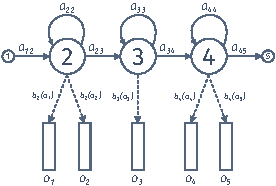
\includegraphics[width=0.7\textwidth]{./ch4-asr/img/hmm_structure.pdf}
  \caption{Příklad levo-pravého Markovova modelu trifónu}
  \label{fig:asr:acoustic:hmm}
\end{figure}

Pokud předpokládáme, že posloupnost slov $W$ je modelována zřetězeným skrytým Markovovým modelem $\lambda$, kde dílčí modely odpovídají fonetickým jednotkám, pak je možné určit pravděpodobnost generování posloupnosti $O$ modelem $\lambda$ jako

\begin{equation}
  P\left(O|\lambda\right) = \sum_{\forall S} P\left(O, S| \lambda\right)P\left(S|\lambda\right) = \sum_{\forall S} a_{s\left(0\right)s\left(1\right)} \prod_{t=1}^{T} b_{s\left(t\right)}\left(o_t\right)a_{s\left(t\right)s\left(t+1\right)},
  \label{eq:asr:acoustic:structure:output}
\end{equation}

\noindent kde posloupnost stavů $S = \left\{s\left(0\right), s\left(1\right),\dots, s\left(T+1\right)\right\}$ je chápána tak, že $s\left(0\right)$ je výstpní a $s\left(T+1\right)$ výstupní neemitující stav modelu $\Theta$ dané promluvy \cite{Psutka2006}. Přitom tento model lze značit trojicí

\begin{equation}
  \lambda = \left[\left\{a_{ij}\right\}_{k,s=1}^{I}; \left\{b_s(.)\right\}_{s=1}^{I};\left\{\pi_{s}\right\}_{s=1}^{I}\right],
  \label{eq:asr:acoustic:structure:marking}
\end{equation}

\noindent kde $a_{ij}$ je přechodová a $b_s(.)$ výstupní pravděpodobnost. Dále $\pi_s$ je rozložení pravděpodobnosti počátečního stavu a $I$ je počet stavů modelu.

Přímé vyčíslení pravděpodobnosti $P\left(O|\lambda\right)$ podle vztahu (\ref{eq:asr:acoustic:state:output}) je z hlediska počtu operací často nerealizovatelné, protože se jedná řádově o $2TN^{T}$ operací násobení. Z tohoto důvodu se proto využívá výpočetně efektivnější tzv. \textbf{algoritmus forward-backward (FB)} s přibližně $N^{2}T$ operací násobení.

Při výpočtu odpředu (forward) se určuje pravděpodobnost $\alpha_j\left(t\right)$ definovaná vztahem

\begin{equation}
  \alpha_{j}\left(t\right) = P\left(o_1o_2\dots o_t, s\left(t\right)=s_j|\lambda\right),
  \label{eq:asr:acoustic:structure:forward}
\end{equation}

\noindent pro výpočet odzadu (backward) se určuje pravděpodobnost $\beta_j\left(t\right)$ definována vztahem


\begin{equation}
  \beta_j\left(t\right) = P\left(o_{t+1}o_{t+2}\dots o_T|s\left(t\right)=s_j|\lambda\right).
  \label{eq:asr:acoustic:structure:backward}
\end{equation}

Podle \cite{Psutka2006} lze snadno dokázat, že výsledná pravděpodobnost $P\left(O|\lambda\right)$ může být vyčíslena vztahem

\begin{equation}
  P\left(O|\lambda\right) = \sum_{s=1}^{N} P\left(O, s\left(t\right) = s | \lambda\right) = \sum_{i = 1}^{N} \alpha_{i}\left(t\right)\beta_{i}\left(t\right)
  \label{eq:asr:acoustic:structure:forward-backward}
\end{equation}

\noindent pro $1 \leq t \leq T$.

\subsection{Trénování parametrů HMM s Gausovkými směsmi}
\label{chap:asr:acoustic:GMM}

Volba struktrury skrytého Markovova modelu je spíše expertní úlohou návrhu. Stanovéní hodnot parametrů modelu je uskutečněno trénováním (odhadem, etimací) na základě trénovacích akustických dat a jejich textových anotací (tzv. korpus). Pro trénování parametrů se využívá tzv. Baum-Welchův interativní algoritmus, což je speciální případ EM algoritmu. Více o něm v \cite{Holmes2001}. Pro odhad střední hodnoty $\mu_{sj}$, tj. složky $m$ gaussovské směsi ve stavu $j$ slouží vztah

\begin{equation}
  \hat{\mu}_{jm} = \frac{\sum_{t=1}^{T}\gamma_{jm}\left(t\right)o_t}{\sum_{t=1}^{T}\gamma_{jm}\left(t\right)},
  \label{eq:asr:acoustic:structure:mu}
\end{equation}

\noindent kde $N$ je počet stavů a $M$ počet složek. Také platí $1 \leq j \leq N$ a $1 \leq m \leq M$. Odhad kovarianční matice $C_{jm}$, tj. složky náležící m-té složce gaussovské směsi ve stavu $j$

\begin{equation}
  \hat{C}_{jm} = \frac{\sum_{t=1}^{T} \gamma_{jm}\left(t\right)\left(o_t - \hat{\mu}_{jm}\right)\left(o_t - \hat{\mu}_{jm}\right)^{T}}{\sum_{t=1}^{T}\gamma_j\left(t\right)},
  \label{eq:asr:acoustic:structure:covariant}
\end{equation}

\noindent kde $1 \leq j \leq N$ a $1 \leq m \leq M$. Odhad váhové složky hustotní směsi $c_{jm}$, tj. složky náležící složce $m$ gaussovské směsi ve stavu $j$ se provádí vztahem

\begin{equation}
  \hat{c}_{jm} = \frac{\sum_{t=1}^{T} \gamma_{jm}\left(t\right)}{\sum_{t=1}^{T}\gamma_j\left(t\right)},
  \label{eq:asr:acoustic:structure:weight}
\end{equation}

\noindent kde $1 \leq j \leq N$ a $1 \leq m \leq M$. Přitom $\gamma_{j}\left(t\right)$ představuje přavděpodobnost, že proces generování posloupnosti $O$ je v čase $t$ ve stavu $j$. Pro vyjádření této pravděpodobnosti $\gamma_{j}\left(t\right)$ platí rovnice (\ref{eq:asr:acoustic:structure:forward-backward}). Pro její definování pak platí vztah

\begin{equation}
 \gamma_{j}\left(t\right) = \frac{P\left(O, s\left(t\right)=j|\lambda\right)}{P\left(O|\lambda\right)} = \frac{\alpha_{j}\left(t\right)\beta_{j}\left(t\right)}{P\left(O|\lambda\right)} ,
  \label{eq:asr:acoustic:structure:gamma}
\end{equation}

\noindent kde $j = 1,\dots,N$ a $t = 1, \dots, T$. Pravděpodobnost, že proces generování posloupnosti $O$ je v čase $t$ ve stavu $j$ a generuje složku $m$ gaussovské hustotní směsi

\begin{equation}
  \gamma_{jm}\left(t\right) = \frac{P\left(O, s\left(t\right)=j, m\left(j,t\right)=m|\lambda\right)}{P\left(O|\lambda\right)} = \frac{\alpha_{j}\left(t\right)\beta_{j}\left(t\right)}{P\left(O|\lambda\right)} \frac{c_{jm}\mathcal{N}\left(o_t;\mu_{jm}; C_{jm}\right)}{\sum_{i=1}^{M} c_{ji} \mathcal{N}\left(o_t;\mu_{ji};C_{ji}\right) }.
   \label{eq:asr:acoustic:structure:gamma:one}
 \end{equation}

\noindent Rozdělení výstupní pravděpodobnosti $b_j\left(o_t\right)$ pro emitující stav $j$ pak má tvar

\begin{equation}
   b_{j}\left(o_t\right) = \sum_{m=1}^{M} \hat{c}_{jm} \mathcal{N}\left(o_t; \hat{\mu}_{jm}; \hat{C}_{jm}\right).
   \label{eq:asr:acoustic:gmm:output}
 \end{equation}

\noindent Akustické modely postavené na kombinaci skrytých Markovových modelů a gaussovských směsí pracují s 10 až 100 tisíc hustotních směsí. Při dimenzi příznakového vektoru (viz \ref{chap:asr:parametrization}) vektoru například $45$ je často nutné provést odhad až 10 miliónů parametrů.

\subsection{Využití neuronových sítí}
\label{chap:asr:acoustic:DNN}

Neuronové sítě se inspirují neuronem v mozku člověka. Ukázka stavby neuronové buňky je znázorněna na obr. \ref{fig:asr:acoustic:dnn:neuron:human}. Dendrity jsou kráktké výběžky, které slouží k příjímání vstupních informací od ostatních neuronů nebo nervů. V tělo neuronu (soma) dochází k reakci na vstupní signály a vytvoření přísušné odezvy. Ta se dále šíří pomocí výběžku nazvaného axon. Jeho délka může dosahovat až 100 cm. Axon je přes synapse spojen s jinými neurony nebo dalšími buňkami v těle.

\begin{figure}[hbpt]
  \centering
  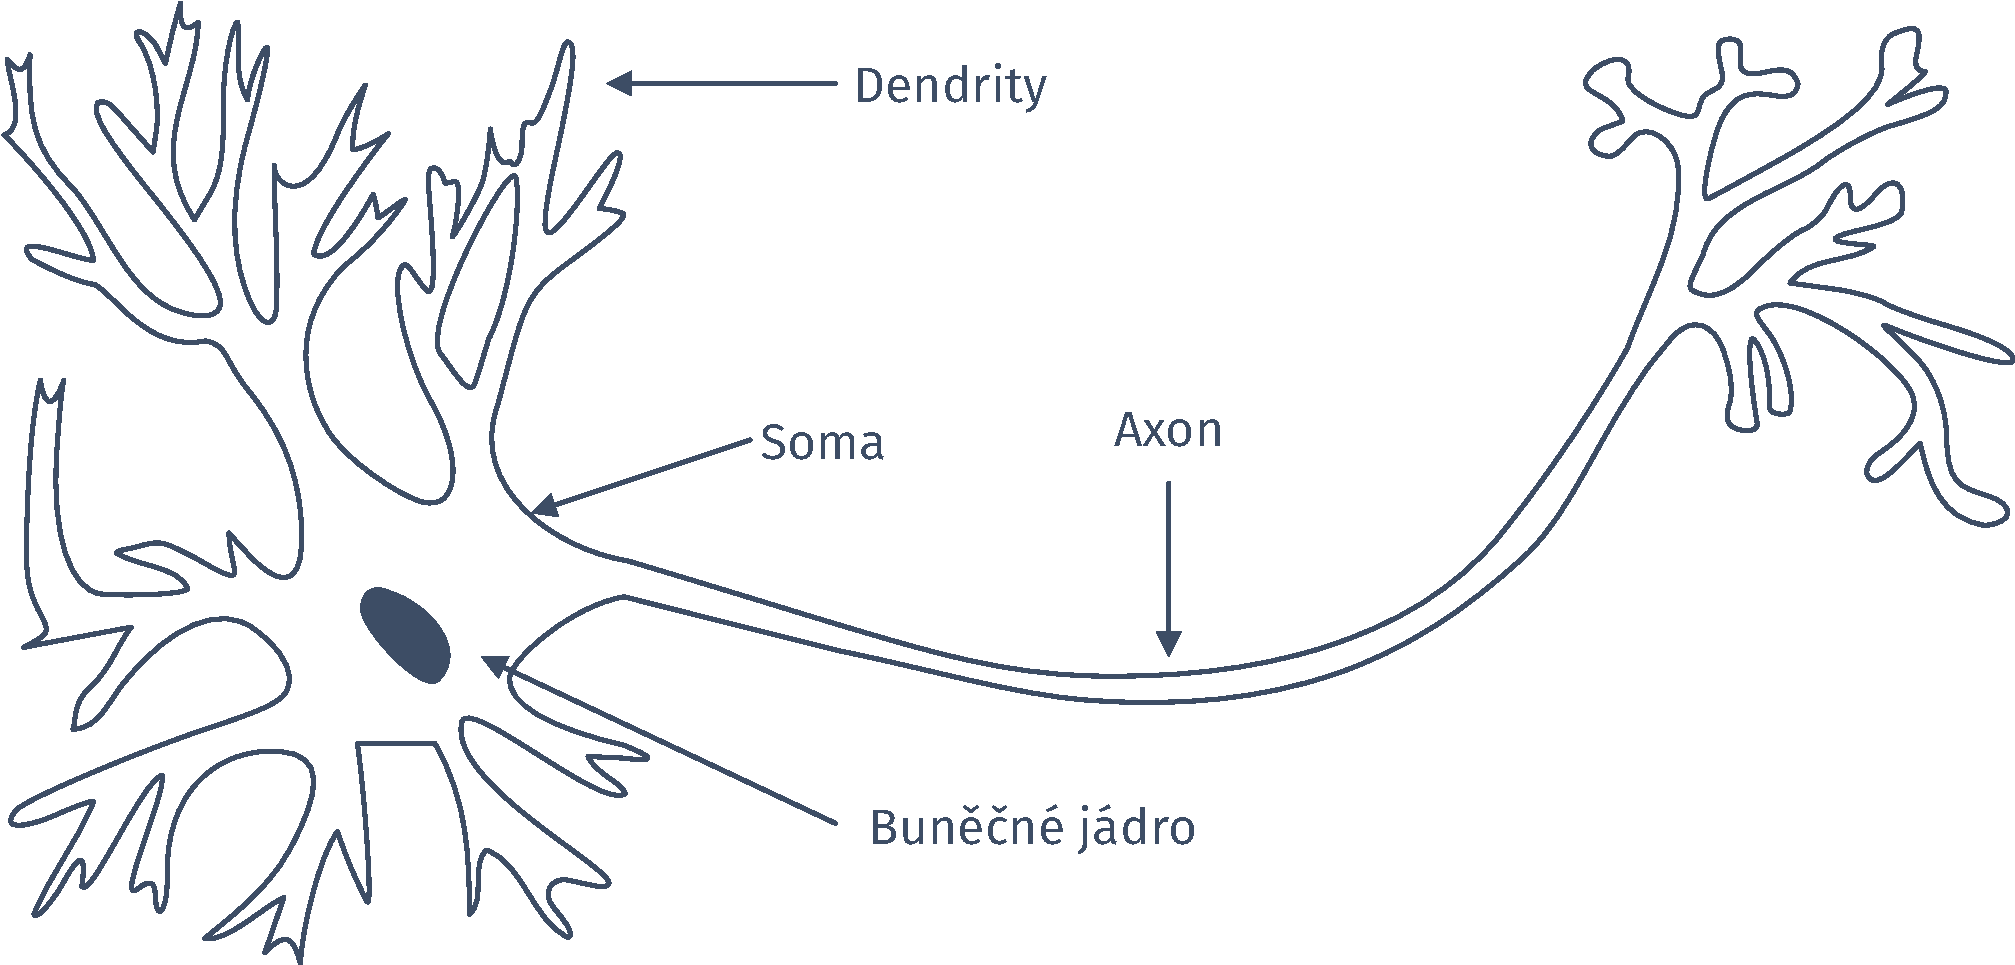
\includegraphics[width=0.7\textwidth]{./ch4-asr/img/neuron-human.pdf}
  \caption{Ukázka neuronové buňky}
  \label{fig:asr:acoustic:dnn:neuron:human}
\end{figure}

Umělý ekvivalent s názvem perceptron byl vytvořen Frankem Roseblattem v první polovině 60. let 20. století \cite{Rosenblatt1962}. Schématicky je zobrazen na obr. \ref{fig:asr:acoustic:dnn:neuron:artificial}. Matematicky lze princip neuronu popsat vztahem

\begin{equation}
  \hat{y}\left(x\right) = \sigma\left(z\right) = \sigma \left(w^{T}x + b\right) = \sigma \left( \sum_{j=1}^{n} w_{j}x_{j} + b\right),
   \label{eq:asr:acoustic:dnn:neuron:output}
 \end{equation}

\noindent kde $x$ představuje vstupní vektor, $w$ váhový vektor a $b$ práh. Výsledek linární kombinace je vstupem aktivační funkce $\sigma\left(.\right)$, jejíž výstup je zároveň výstupem neuronu. Neuronová síť\footnote{Popisovaná neuronová síť je typu feedforward (FF). Dalšími typy sítí jsou konvoluční a rekurentní neuronové sítě. Oproti FF síti se liší hlavně svou strukturou. Princip propojení neuronových buněk je však stejný.} (NN, viz obr. \ref{fig:asr:acoustic:dnn:training}) je složena z jedné či více vrtev neuronů. V případě více vrstvé NN jsou vždy propojeny neurony mezi vrstavami $l$ a $l+1$.

\begin{figure}[hbpt]
  \centering
  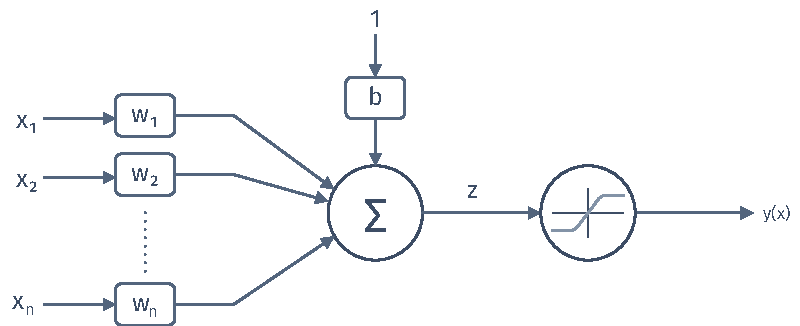
\includegraphics[width=0.7\textwidth]{./ch4-asr/img/neuron.pdf}
  \caption{Schéma perceptronu}
  \label{fig:asr:acoustic:dnn:neuron:artificial}
\end{figure}

Zmíněná aktivační funkce hraje velmi významnou roli, protože umožňuje řešení i nelineárních problémů. Pokud by NN nevyužívala aktivační funkce, jednalo by se defakto stále o lineární kombinaci vektorů a tím pádem by bylo možné řešit jen linární problémy. Mezi nejčastěji používané patří \textit{sigmoid} ($\sigma\left(z\right) = \left(1 - e^{-z}\right)^{-1}$), \textit{tanh} a \textit{relu} ($\sigma\left(z\right) = \max\left(0, z\right)$). Průběhy těchto aktivačních funkcí jsou vidět na obr. \ref{fig:asr:acoustic:dnn:activation}.

 \begin{figure}[htpb]
  \centering
  \begin{subfigure}[b]{0.29\textwidth}
    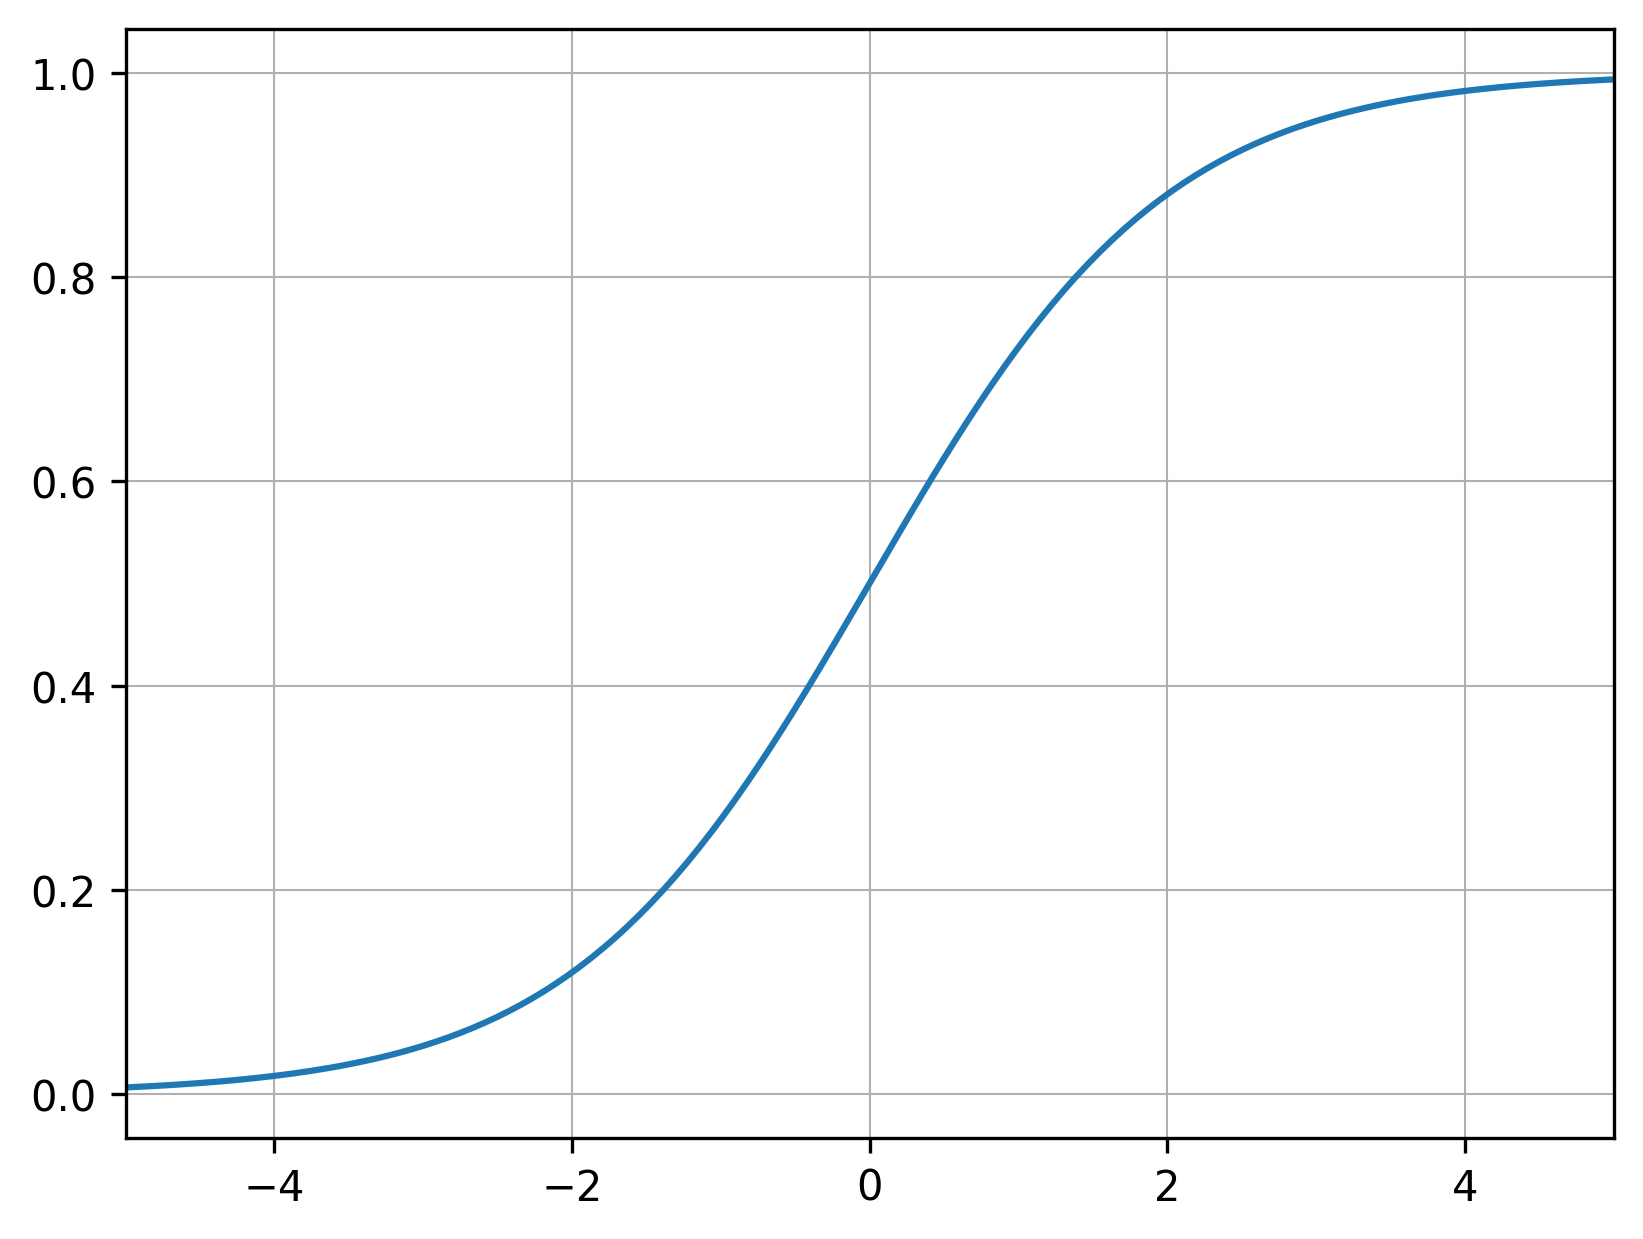
\includegraphics[width=\textwidth]{./ch4-asr/img/sigmoid.png}
    \caption{sigmoid}
    \label{fig:asr:acoustic:dnn:activation:sigmoid}
  \end{subfigure}
  %
  \begin{subfigure}[b]{0.3\textwidth}
    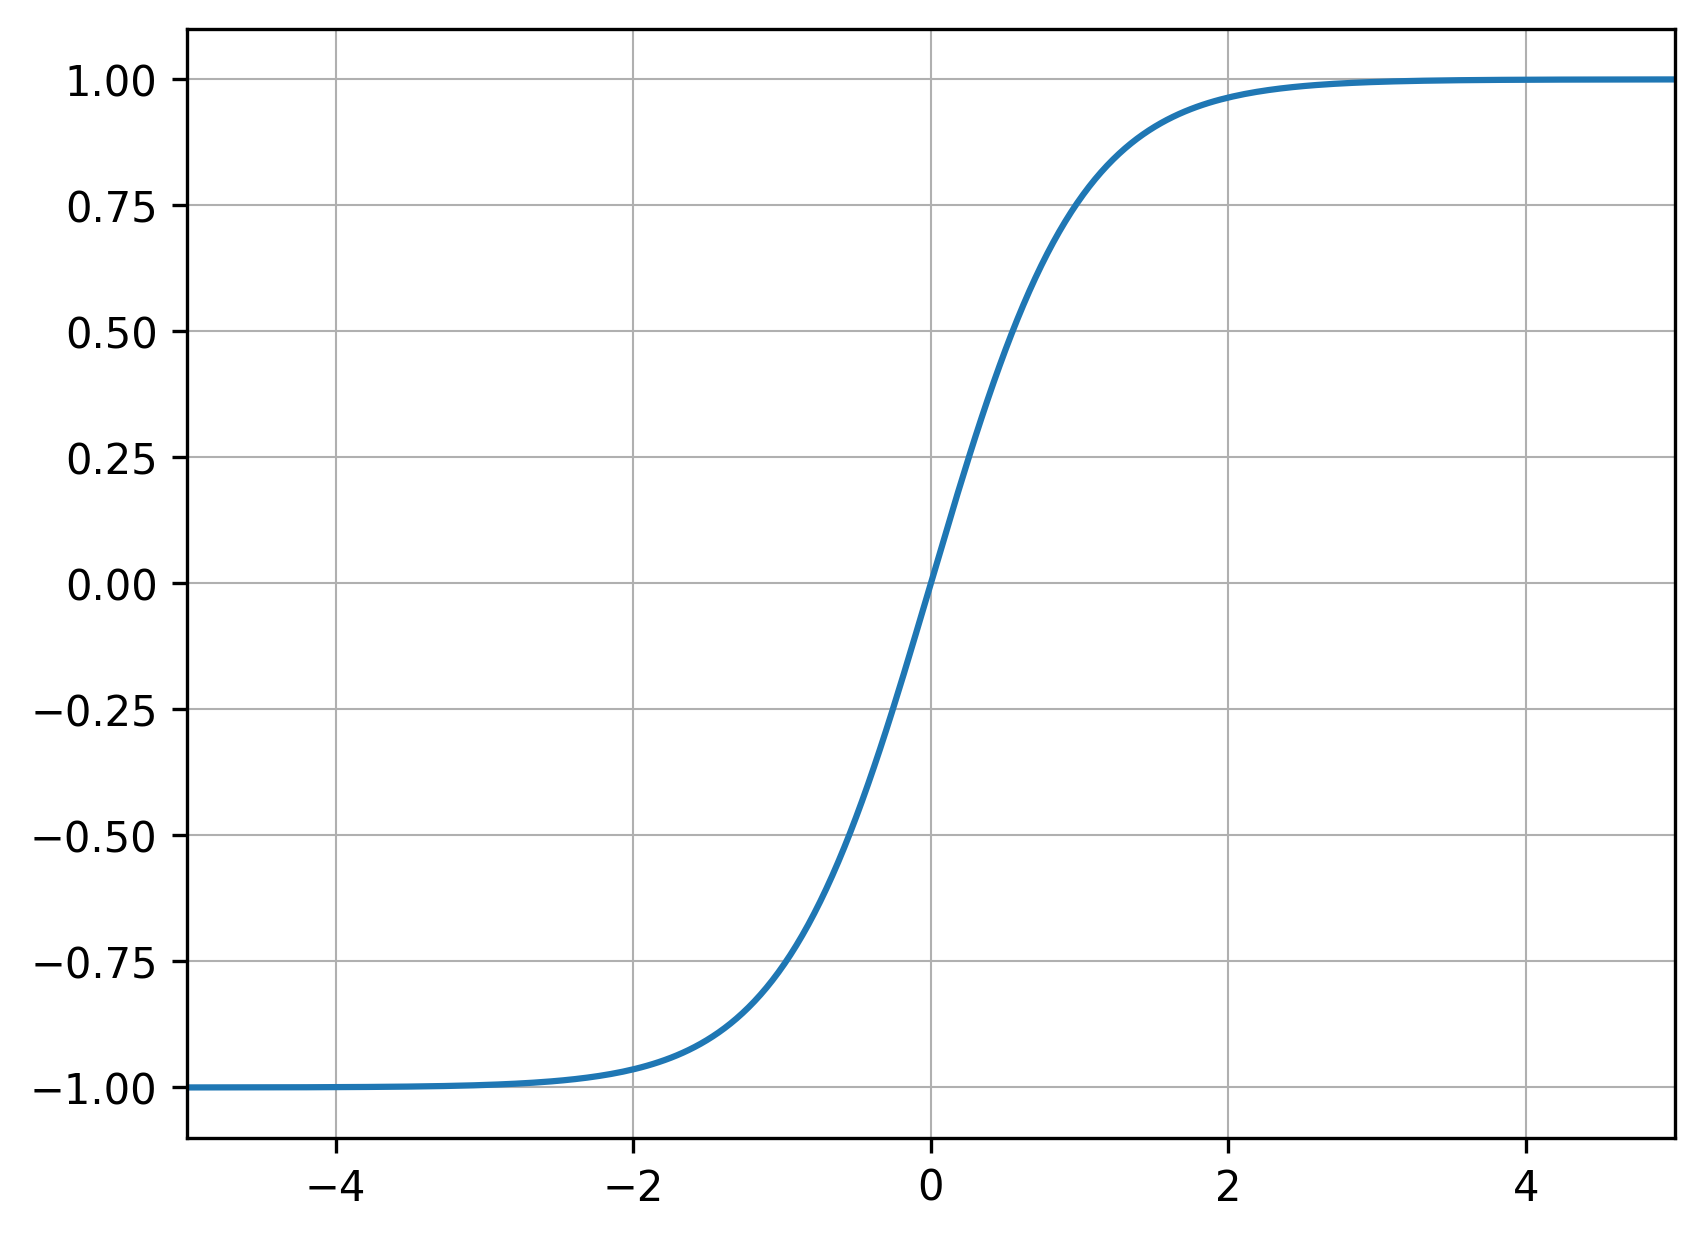
\includegraphics[width=\textwidth]{./ch4-asr/img/tanh.png}
    \caption{tanh}
    \label{fig:asr:acoustic:dnn:activation:tanh}
  \end{subfigure}
  %
  \begin{subfigure}[b]{0.28\textwidth}
    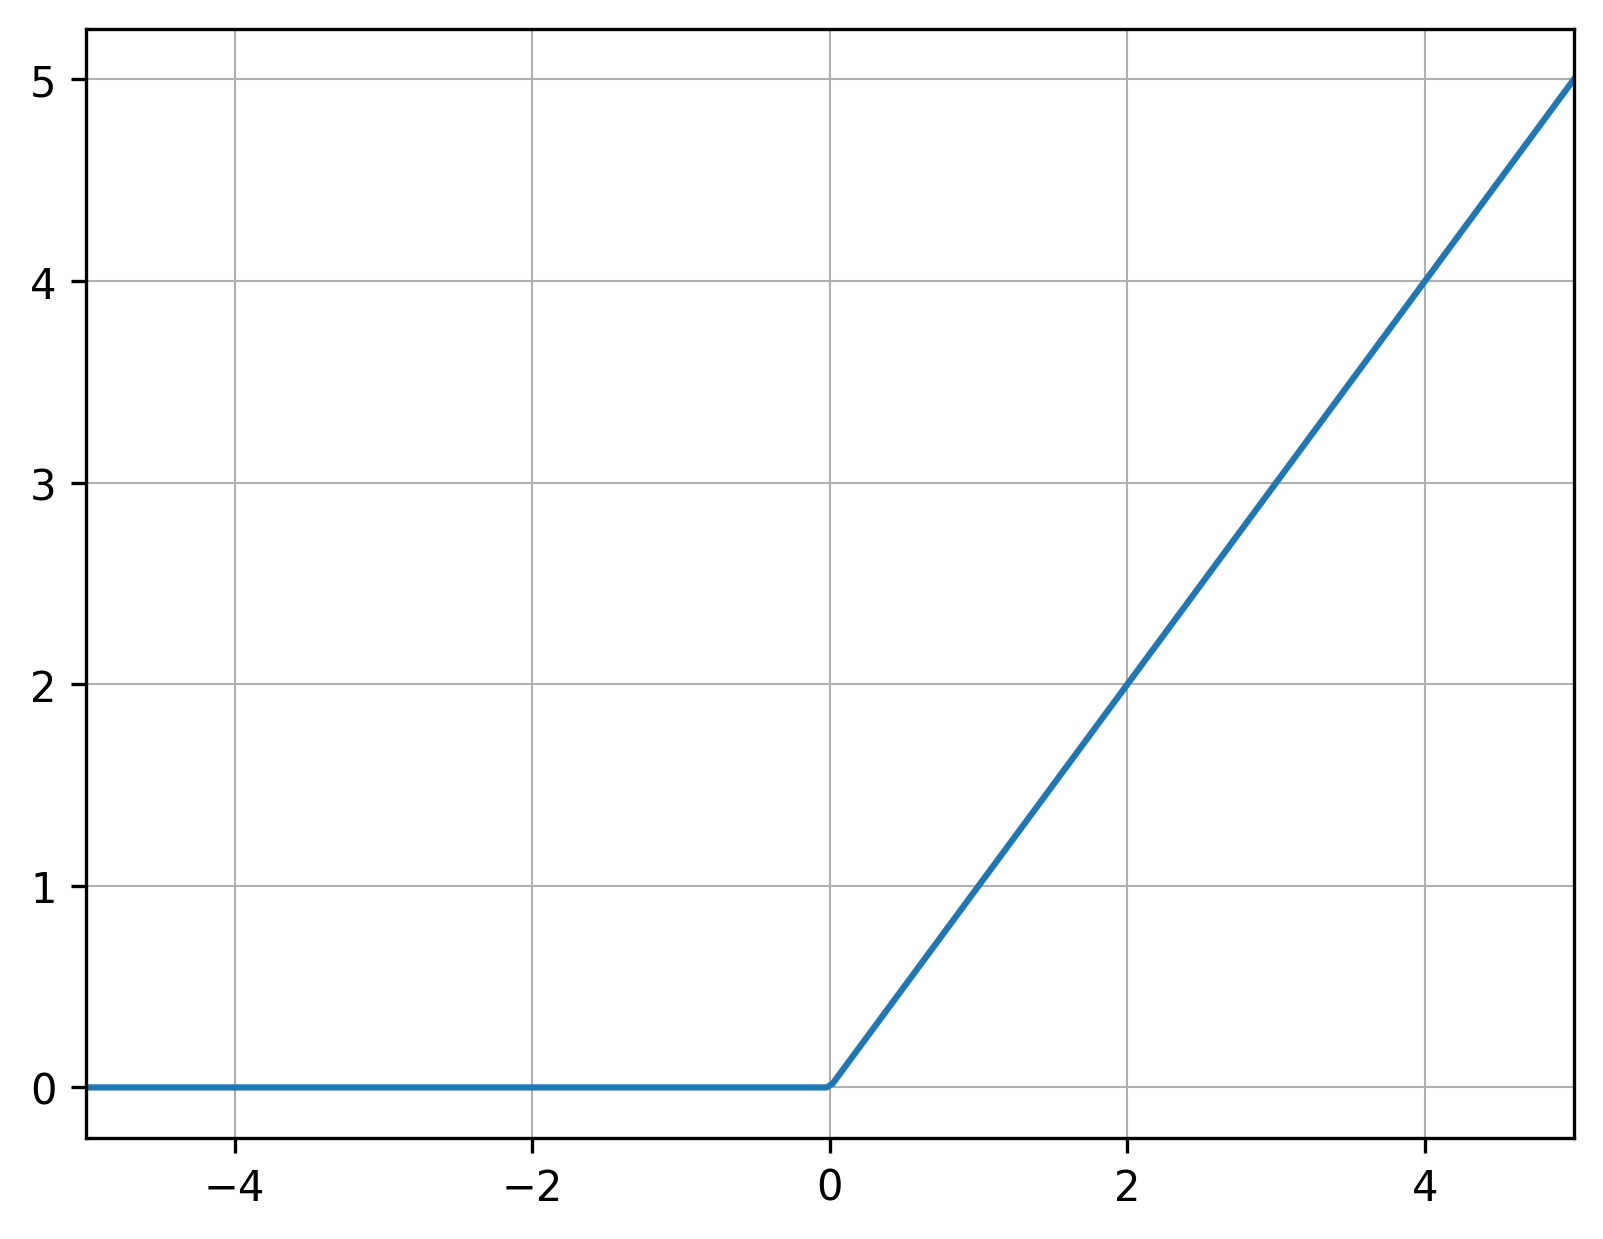
\includegraphics[width=\textwidth]{./ch4-asr/img/relu.png}
    \caption{relu}
    \label{fig:asr:acoustic:dnn:activation:relu}
  \end{subfigure}
  \caption{Příklady používaných aktivačních funkcí}
  \label{fig:asr:acoustic:dnn:activation}
\end{figure}

Pro výpočet výstupu neuronové sítě, tzv. \textbf{forward propagation}, je použit iterativní postup matematicky zapsán jako

\begin{align}
  \begin{split}
    Z^{[l]} = W^{[l]}a^{[l-1]} + b^{[l]}, \\
    a^{[l]} = \sigma^{[l]}\left(Z^{[l]}\right),
  \end{split}
  \label{eq:asr:acoustic:dnn:fw}
\end{align}

\noindent kde $a^{[l]}$ představuje výstup $l$-té vrstvy ($a^{[0]} = x$), $W^{[l]}$ představuje váhovou matici $l$-té vrstvy, $b^{[l]}$ vektor prahů $l$-té vrstvy a $\sigma^{[l]}(.)$ aktivační funkci $l$-té vrstvy. Pro $l$ platí $l = 1, \dots, N$, kde $N$ je počet vrstev neuronové sítě. Výsledkem iterativního výpočtu (\ref{eq:asr:acoustic:dnn:fw}) je výstup sítě $y = a^{[N]}$.

Trénováním neuronové sítě je myšleno určení hodnot váhových matic $W^{[l]}$ a prahů $b^{[l]}$. Tento proces se iterativně sestává ze 3 kroků (viz obr. \ref{fig:asr:acoustic:dnn:training})

\begin{enumerate}
  \item výpočet výstupu sítě (\ref{eq:asr:acoustic:dnn:fw}),
  \item vypočtení chyby predikce $J\left(y, \hat{y}\right)$,
  \item aktualizace vah pomocí algoritmu backpropagation.
\end{enumerate}

\noindent Výpočet výstupu NN je realizován pomocí (\ref{eq:asr:acoustic:dnn:fw}), dále tedy nezbytné vypočítat chybu predikce $J\left(y, \hat{y}\right)$, Ta je difinována vztahem

\begin{equation}
  J\left(y, \hat{y}\right) = \frac{1}{m} \sum_{i=1}^{m}\mathcal{L}\left(y, \hat{y}\right),
  \label{eq:asr:acoustic:dnn:cost}
\end{equation}

\noindent kde $m$ je počet prvků trénovací množiny a $\mathcal{L}\left(y, \hat{y}\right)$ je funkce výpočtu chyby predikce $m$-tého prvku trénovací množiny. Konkrétní funkce závisí na typu řešené úlohy, ale často se používá cross-entropie definované vztahem

\begin{equation}
  \mathcal{L}\left(y, \hat{y}\right) = - \sum_{i=1}^{m} y_i \log \hat{y}_i,
  \label{eq:asr:acoustic:dnn:cost}
\end{equation}

\noindent kde $m$ je dimenze výstupního vektoru.

Samotná aktualizace parametrů sítě je realizování \textbf{backpropagation} algoritmem. Cílem tohoto algoritmu je vypočtení parciálních derivací $\partial J / \partial W^{[l]}$ a $\partial J/\partial b^{[l]}$. Tyto parciální derivace je potřeba vypočíst pro všechny vrstvy sítě. Chyba ve vrstvě $l$ je závislá na chybě v předchozí vrstvě $l-1$. Tato skutečnost znamená, že je možné použít tzv. chain pravidlo. Parciální derivace pak mají následující podobu

\begin{align}
  \begin{split}
    \frac{\partial J}{\partial W^{[l]}} & = \frac{\partial J}{\partial a^{[l]}} \frac{\partial a^{[l]}}{\partial z^{[l]}} \frac{\partial z^{[l]}}{\partial W^{[l]}}, \\
    \frac{\partial J}{\partial b^{[l]}} & = \frac{\partial J}{\partial a^{[l]}} \frac{\partial a^{[l]}}{\partial z^{[l]}} \frac{\partial z^{[l]}}{\partial b^{[l]}}
  \end{split}
  \label{eq:asr:acoustic:dnn:partial}
\end{align}

\noindent Vzorce pro výpočet aktualizací parametrů sítě jsou pak následující

\begin{align}
  \begin{split}
    \delta^{[L]} & = \nabla_{a} J \odot \sigma'\left(z^{[L]}\right), \\
    \delta^{[l]} & = \left(\left(w^{[l+1]}\right)^T \delta^{[l+1]}\right) \odot \sigma'\left(z^{[l]}\right), \\
    \frac{\partial J}{\partial W^{[l]}} & = a^{[l-1]}\delta^{[l]}, \\
    \frac{\partial J}{\partial b^{[l]}} & = \delta^{[l]},
  \end{split}
  \label{eq:asr:acoustic:dnn:bp}
\end{align}

\noindent kde $\nabla_a J = \partial J / \partial a^{[L]}$ a $\odot$ představuje Hadamardův součin. Samotná aktualizace parametrů je realizována vztahy

\begin{align}
  \begin{split}
    W^{[l]} & = W^{[l]} - \alpha \frac{\partial J}{\partial W^{[l]}}, \\
    b^{[l]} & = b^{[l]} - \alpha \frac{\partial J}{\partial b^{[l]}},
  \end{split}
  \label{eq:asr:acoustic:dnn:update}
\end{align}

\noindent kde $\alpha$ reprezentuje koeficient učení.

\begin{figure}[hbpt]
  \centering
  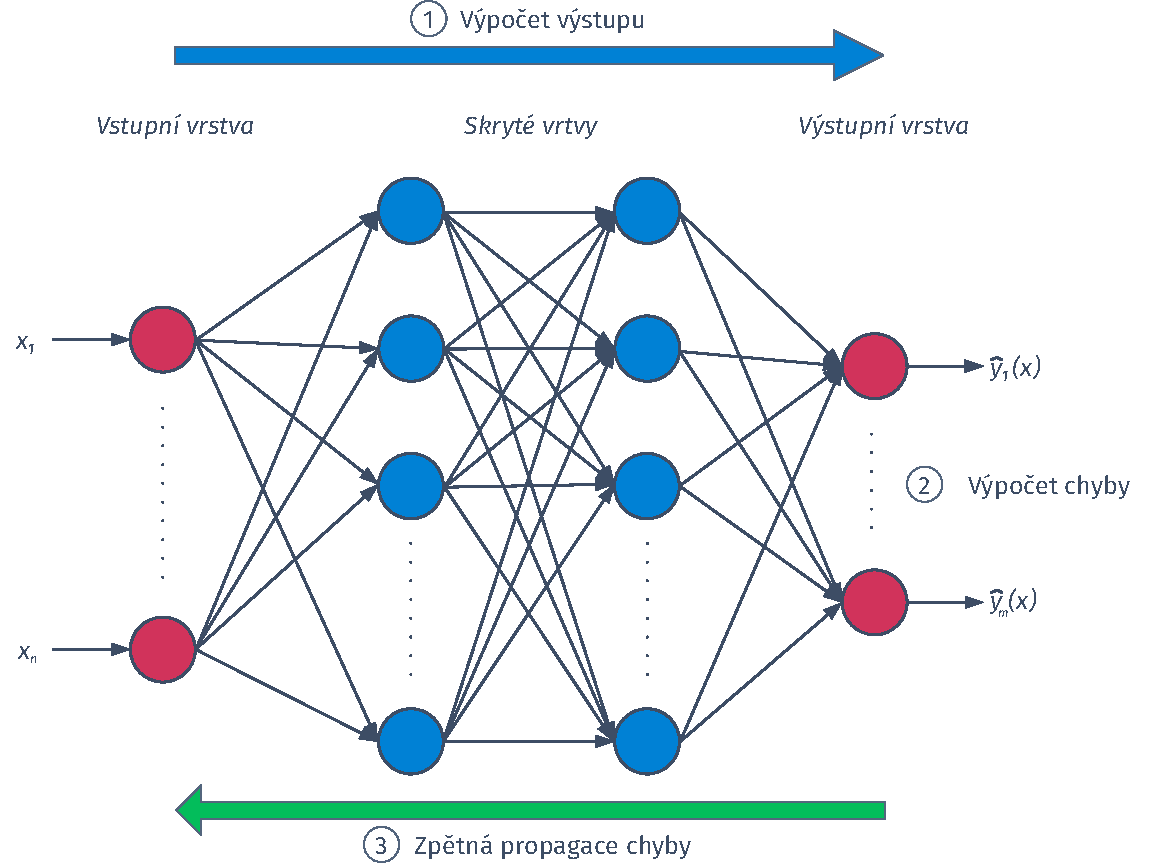
\includegraphics[width=0.9\textwidth]{./ch4-asr/img/dnn-training.pdf}
  \caption{Schéma a princip učení neuronové sítě}
  \label{fig:asr:acoustic:dnn:training}
\end{figure}

\subsubsection{Spojení skrytých Markovových modelů a neuronových sítí}

Rozvoj výpočetní techniky, zejména GPU\footnote{Graphics Processing Unit} s možností provádět obecné maticové operace, zapříčinil masivní využití tzv. hlubokých neuronových sítí (DNN). Ty se vyznačují vyšším počtem skrytých vrstev, což umožňuje řešit sofistikovanější problémy. Jedním takovým je rozpoznávání souvislé řeči. Bohužel DNN end-to-end\footnote{Systém, který kompletně řeší rovnici (\ref{eq:asr:decoding:generic}) pomocí jediné DNN sítě. Tyto systémy jsou většinou postaveny na rekurentních neuronových sítích (RNN).} systém je zatím velmi komplikované vytvořit a provozovat zejména, proto že k uspěšnému natrénování je potřeba řádově více dat, než u GMM \cite{Amodei2016}. Z tohoto důvodu jsou v současné době nejčastější systémy postavené na kombinaci HMM a DNN (HMM-DNN). Rozdíl oproti end-to-end systému je v tom, že cílem DNN není odhad $\hat{W}$, ale ,stejně jako v případě HMM-GMM, určit $b_j\left(o_t\right)$.

V případě HMM-GMM je odhad $b_j\left(o_t\right)$ realizován gaussovskými hustotními směsmi podle vzorce (\ref{eq:asr:acoustic:gmm:output}). Těchto směsí je tolik, kolik je unikátních stavů HMM. U DNN však žádné směsi k dispozici nejsou. Pokud je všask výstupní vrstva typu \textbf{softmax}, kde výstup $j$-tého neuronu je definován vztahem

\begin{equation}
  y_{j} = a_{j}^{[L]} = \frac{e^{z_j}}{\sum_{i=1}^{m}e^{z_i}},
  \label{eq:asr:acoustic:dnn:asr:softmax}
\end{equation}

\noindent kde $m$ je počet neuronů v poslední vrstvě. Zároveň platí

\begin{equation}
  \sum_{j=1}^{m} y_{j} = 1.
  \label{eq:asr:acoustic:dnn:asr:softmax:criterium}
\end{equation}

\noindent Hodnoty výstupního vektoru $y$ mají pseudo-pravděpodobnostní charakter. Pokud tedy bude $m$ rovno počtu stavů $HMM$, pak výstupní pravděpodnost $b_{j} \left(o_t\right)$ pro emitující stav $j$ má, podle (\ref{eq:asr:acoustic:dnn:asr:softmax}), tvar

\begin{equation}
  b_{j} \left(o_t\right) = y_{j} = \frac{e^{z_j}}{\sum_{i=1}^{m}e^{z_i}}.
  \label{eq:asr:acoustic:dnn:asr:softmax:criterium}
\end{equation}

\noindent Principiální rozdíl ve funkci HMM-GMM a HMM-DNN je znázorněn na obr. \ref{fig:asr:acoustic:dnn:asr:diff}.

\begin{figure}[htpb]
  \centering
  \begin{subfigure}[b]{0.4\textwidth}
    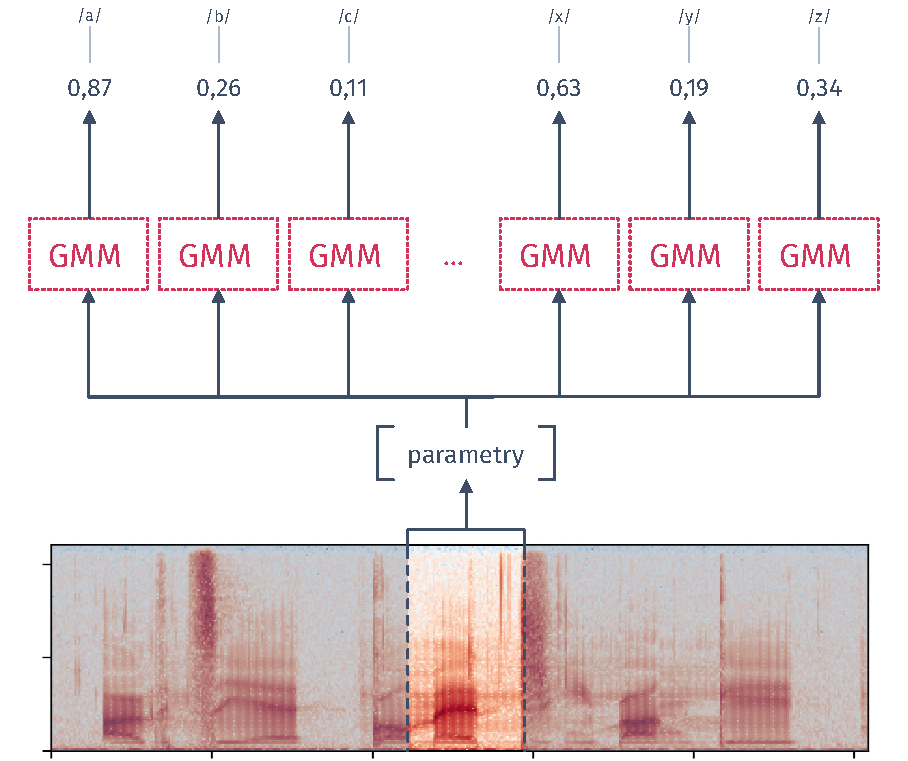
\includegraphics[width=\textwidth]{./ch4-asr/img/hmm-gmm.pdf}
    \caption{GMM}
    \label{fig:asr:acoustic:dnn:asr:diff:dnn}
  \end{subfigure}
  %
  \begin{subfigure}[b]{0.4\textwidth}
    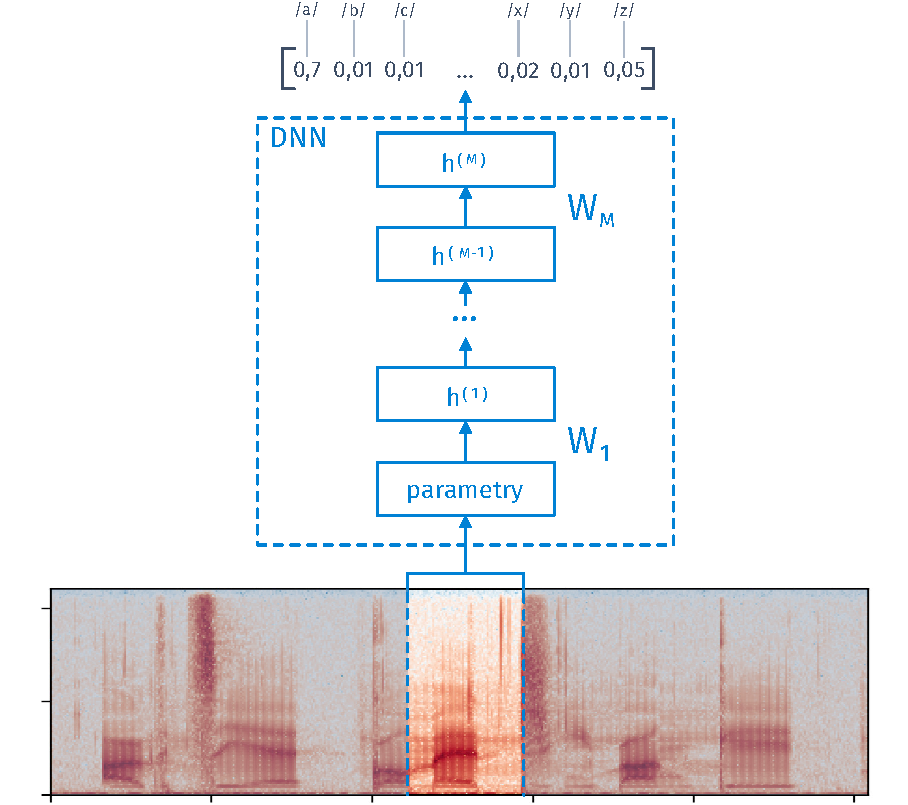
\includegraphics[width=\textwidth]{./ch4-asr/img/hmm-dnn.pdf}
    \caption{DNN}
    \label{fig:asr:acoustic:dnn:asr:diff:dnn}
  \end{subfigure}
  \caption{Principální rozdíl ve funkci GMM a DNN systému}
  \label{fig:asr:acoustic:dnn:asr:diff}
\end{figure}

K natrénování DNN se používá zmíněného backpropagation algoritmu. V poslední době se však prosadilo trénování využívající předtrénování DNN pomocí tzv. restricted Bolzmann machines (RBM) \cite{Hinton2012}. Předtrénování řeší problém kdy se informace zpětně propagovaná pomocí backpropagation algoritmu úplně neovlivní počáteční vrstvy, protože gradient je příliš malý. Předtrénování pomocí RBM pomáhá lépe určit parametry sítě. Princpálně je tento proces znázorněn na obr. \ref{fig:asr:acoustic:dnn:pretraining}.

Nejprve je natrénován GRBM (Gaussian-Bernoulli RBM) model na mikrosegmentu řeči složeného z několika okének parametrů odpovídající délce promluvy například $10\ ms$. Stav skrytých jednotek je použit k natrénování RBM. Tento proces se opakuje dokud není natrénován požadovaný počet vrstev výsledné sítě. Následně jsou jednotlivé RBM spojeny do deep belief sítě (DBN). Následně je přidána výstupní softmax vrstva dimenze rovné počtu HMM stavů (DBN-DNN). Tato DBN-DNN síť je pak diskriminativně trénována na základě zarovnání získaného pomocí HMM-GMM. Více o tomto principu trénování v \cite{Hinton2012} a \cite{Vesely2013}. Vstupem neuronové sítě je často mikrosegment $t$ a jeho okolní mikrosegmenty. Velmi často se používá okolí $t-2$ a $t+2$.

\begin{figure}[hbpt]
  \centering
  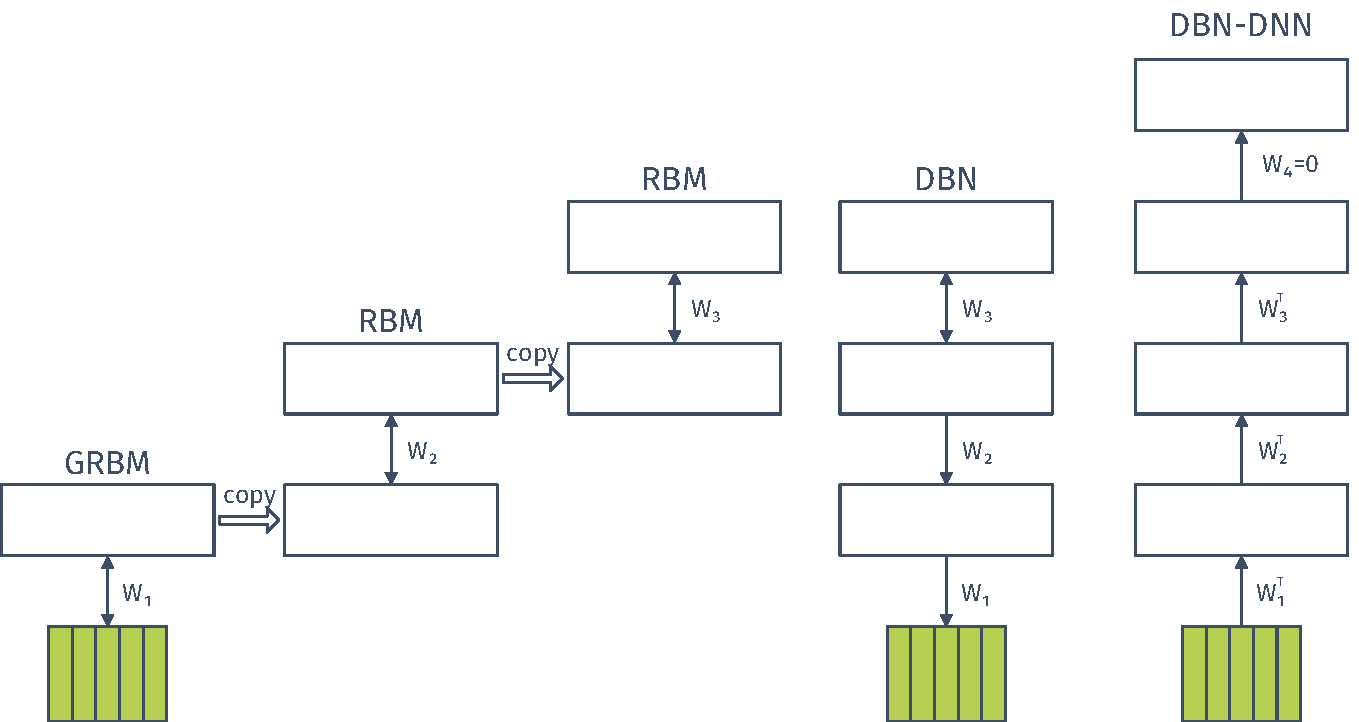
\includegraphics[width=0.9\textwidth]{./ch4-asr/img/pretraining.pdf}
  \caption{Princip předtrénování pomocí RBM s třemi vrstvami \cite{Hinton2012}.}
  \label{fig:asr:acoustic:dnn:pretraining}
\end{figure}

\subsubsection{Time-delay neural networks}

Nevýhodou DNN sítí je, že berou v potaz pouze statické parametry v rámci zpracovávaných mikrosegmentů, protože sumace v perceptronu odpovídá sumě vážených statických vstupů. Po zpracování segmentu $t$ není získaná informace nijak reflektována při zpracování segmentu $t+1$. Tento nedostatek by řešilo použití rekurentních neuronových sítí (RNN). Bohužel tyto sítě mají mnohem komplikovanější buňku neuronu než FF sítě s perceptronem \cite{Amodei2016}. Proto je potřeba řádově více dat k natrénování. Složitost buňky také zvyšuje komputační náročnost výpočtu.

Základním rozdílem sítí typu time-delay neural network (TDNN) (představená v \cite{Waibel1989}) je přidání časové filtrace do sumační části neuronu, tím je docíleno zahrnutí dynamické složky do výpočtu sítě \cite{Craig2000}. Filtrace je implementována jako filtr s konečnou impulzní odezvou (FIR), tedy

\begin{equation}
  z_{j}^{[l]}\left(t\right) = \sum_{n=0}^{N} w_{j}^{[-n]}f\left(n\right)a^{[l-1]}\left(t - n\right) + b_{j},
  \label{eq:asr:acoustic:dnn:tdnn:fir}
\end{equation}

\noindent kde $t$ je dikrétní časový index, $N$ je délka FIR filteru, $f\left(n\right)$ odezva filtru, $w_{j}^{[-n]}$ příslušná váha, $a^{[l-1]}$ je výstup vrstvy $l-1$ a $z_{j}^{[l]}\left(t\right)$ je výstup sumační části neuronu $j$ ve vrstvě $l$. Vztah (\ref{eq:asr:acoustic:dnn:tdnn:fir}) tedy představuje konvoluci. Na obr. \ref{fig:asr:acoustic:dnn:tdnn:neuron} je principiálně znázorněn neuron pracující s $N$ FIR filtry. Z obr. \ref{fig:asr:acoustic:dnn:tdnn:neuron} je také zřejmé, že TDNN síť má několik souborů vah $W^{x}$, které umožňují lépe pracovat s dynamickou složkou signálu \cite{Peddinti2015}.

\begin{figure}[htpb]
  \centering
  \begin{subfigure}[b]{0.45\textwidth}
    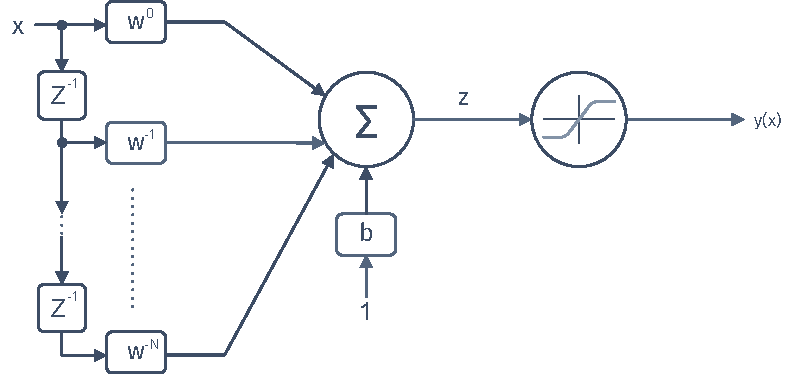
\includegraphics[width=\textwidth]{./ch4-asr/img/neuron-tdnn.pdf}
    \caption{neuron}
    \label{fig:asr:acoustic:dnn:tdnn:neuron}
  \end{subfigure}
  %
  \begin{subfigure}[b]{0.35\textwidth}
    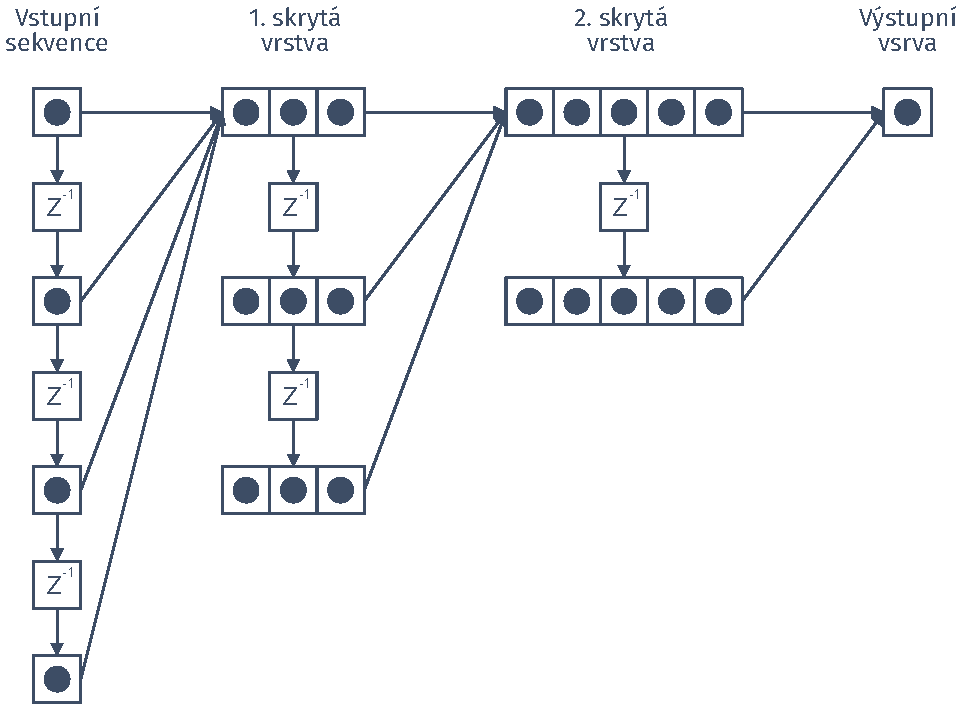
\includegraphics[width=\textwidth]{./ch4-asr/img/tdnn.pdf}
    \caption{síť}
    \label{fig:asr:acoustic:dnn:tdnn:net}
  \end{subfigure}
  \caption{Neuron TDNN sítě a jednoduché blokové schéma TDNN sítě \cite{Craig2000}}
  \label{fig:asr:acoustic:dnn:tdnn}
\end{figure}

Stejně jako v případě DNN sítě je vstupem parametrizovaný mikrosegment $t$ a jeho okolí. Z obr. \ref{fig:asr:acoustic:dnn:tdnn:net} je patrné, že hlubší vsrtvy postupně zpracovávájí větší a větší okolí mikrosegmentu $t$. Dimenze výstupní vrstvy odpovída počtu HMM stavů. Přestože je TDNN síť typu FF, tak dokáže pracovat i s dynamickými parametry řeči, protože využívá princip konvoluce.

% !TEX root = ../thesis.tex
\section{Jazykové modelování}
\label{chap:asr:language}

Jazykový model (obr. \ref{fig:asr:decoding}) je po parametrizaci a akustickém modelu další důležitou částí systému rozpoznávání řeči. Jeho úkolem je poskytnout dekodéru co nejrychleji nejpřesnější odhad apriorní pravděpodobnosti $P\left(W\right)$ pro libovolnou posloupnost slov $W$. Tuto pravděpodonost je možné vyjádřit vztahem

\begin{equation}
  P\left(W\right) = \prod_{k=1}^{K} P\left(w_k | w_{k-1}\dots w_{1}\right),
  \label{eq:asr:language:W_full}
\end{equation}

\noindent kde $K$ je počet slov posloupnosti $W$. Pokud by byl proveden rozklad (\ref{eq:asr:language:W_full}) vyšlo by najevo, že pravděpodobnost výskytu slova $P\left(w_i\right),\ i \leq K$ je podmíněna pouze svou historií, tj. posloupností slov $w_1\ \dots\ w_{i-2}w_{i-1}$.

Systémy rozpoznávání řeči pracují obvykle s rozsáhlými slovníky, čítající stovky tisíc až jednotky milionů slov, není možné předpokládat, že by bylo možné pravděpodobnosti v (\ref{eq:asr:language:W_full}) dostatečně robustně odhadnout pro libovolnou délku posloupnosti $K$.

Obvykle se proto provádí aproximace vztahu (\ref{eq:asr:language:W_full}), při níchž docházi k redukci počtu odhadovaných parametrů. Nejčastějším způsobem je stanovení ekvivalentních tříd slov na základě jejich slovní historie, tj. všechny historie $w_1\ \dots\ w_{i-2}w_{i-1}$, které se shodují v posledních $n-1$ slovech, jsou zařazeny do stejné třídy. Uvedené modely se nazývají \textbf{n-gramové modely}. Přitom \textit{n}-gramem se rozumí posloupnost $n$ za sebou jdoucích slov v pozorování jejich náhodného výběru, např. trénovacího korpusu obsahujícího textová data. Modely s $n=0$ se nazývají \textbf{zerogramy}, $n=1$ pak \textbf{unigramy}. Nejpoužívanější jsou pak \textbf{bigramy} ($n=2$) a \textbf{trigramy} ($n=3$). Pravděpodobnost $P\left(W\right)$ u $n$-gramového modelu se vypočte vztahem

\begin{equation}
  P\left(W\right) = \prod_{k=1}^{K} P\left(w_k | w_{k-1}\dots w_{k-n+1}\right).
  \label{eq:asr:language:W}
\end{equation}

\noindent V ideálním případě by optimální model měl mít $n > 3$, ale v praxi se tyto modely moc nepoužívají, protože s rostoucím řádem modelu enormně roste potřebná velikost trénovacích dat. Například pro slovník s $N$ položkami existuje stále $N^{n}$ $n$-gramových statistik, které je potřeba odhadnout. Jak bylo zmíněno odhad těchto statistik se provádí na základě relativních četností v trénovacích datech. Například u bigramů ($n=2$) a slovníku o velikosti $N=10^{5}$ je zapotřebí odhadnout $10^{10}$ různých bigramů a k tomu je zapotřebí relativně velké trénovací množiny. Je zřejmé, že většina z těchto $10^{10}$ bigramů se vůbec neobjeví v datech. Těmto \uv{neviděným} bigramům tedy odpovídá nulová pravděpodobnost, což vyústí v nulovou pravděpodobnost $P\left(W\right)$ (\ref{eq:asr:language:W}). K řešení tohoto problému se používá technik \uv{vyhlazování}. Jejich cílem je odhad pravděpodobností těchto neviděných jevů s využitím tzv. ústupových, interpolačních a diskontních schémat \cite{Psutka2006}.

Výstupem akustického modelu jsou většinou fonémy ve zvolené fonetické abecedě (např. SAMPA). Nezbytnou součástí systémů rozpoznávání řeči, tak je výslovnostní slovník, který obsahuje kombinace slov a fonetického přepisu těchto slov.
%Z principu může mít jedno slovo více fonetických transkripcí.
Tento slovník umožňuje výpočet $P\left(W\right)$ na základě výstupu akustického modelu.

% !TEX root = ../thesis.tex
\section{Dekódování}
\label{chap:asr:decoding}

Hlavní funkcí dekodéru je nalezení jedné nejlepší nebo více vhodných výstupních posloupností slov $\hat{W}$.
% Matematicky lze tento proces popsat pomocí vztahu
% \begin{equation}
%   \hat{W} = \argmax_{W} P\left(\boldsymbol{O} | W\right)P\left(W\right),
%   \label{eq:asr:decoding:decoder}
% \end{equation}
% \noindent kde $P\left(\boldsymbol{O}|W\right)$ představuje již popsaný akustický model, $P\left(W\right)$ opisuje jazykový model. V~některých případech je úloha dekódování zobecněna na nalezení více než jedné posloupnosti slov $\hat{W}$.
% Pokud je posloupností více, tak se mluví jako o hledání \textbf{\textit{N} nejlepších} (\textit{N}-best) posloupností slov $\hat{W}$.
% Řešení této úlohy je netriviální, protože dekodér obvykle nemá informaci o počtu slov v~dané promluvě, protože ASR systémy nevyžadují vyslovování pauz mezi jednotlivými slovy. Navíc, i kdyby tato informace byla  k~dispozici, tak pro promluvu, která čítá $M$ slov, je se slovníkem čítajícím $N$ slov, potřeba prozkoumat $N^{M}$ různých slovních kombinací (hypotéz), tj. například $10^{50}$ vyhodnocení při $N=100000$ a $M=10$. Z toho jasně plyne, že aplikace metody vyčerpávajícího prohledávání je i pro úlohu s~malými slovníky a krátkými promluvami nerealizovatelná.
% Naštěstí bylo navrženo několik účinných algoritmů, které řeší úlohu hledání maxima (\ref{eq:asr:decoding}) bez exponenciálního nárůstu počtu výpočtů.
Mezi takové algoritmy patří dekódování podle \textbf{kritéria maximální aposteriorní pravděpodobnosti (MAP)}, nebo v~současnosti primárně používaného dekódování podle \textbf{Viterbiova kritéria}.

% Akustický model zjišťuje pravděpodobnost $P\left(\boldsymbol{O}|W\right)$, resp. $P\left(\boldsymbol{O}|\lambda\right)$ pomocí forward-backward (FB) algoritmu.
% Ten pro pozorovanou posloupnost $\boldsymbol{O}$ určí pravděpodobnosti všech možných cest délky $T$ modelem $\lambda$.
% Výpočet podmíněné pravděpodobnosti lze aproximovat pravděpodobností $P_S(\boldsymbol{O}|\lambda)$, reprezentující nejpravděpodobnější posloupnost HMM stavů, kterými projde posloupnost $\boldsymbol{O}$ modelem $\lambda$, tedy

% \begin{equation}
%   P\left(\boldsymbol{O}|\lambda\right) \approx P_S\left(\boldsymbol{O}|\lambda\right) = \max_S P\left(\boldsymbol{O}, S| \lambda \right) = \max_S a_{s\left(0\right)s\left(1\right)} \prod_{t=1}^{T} b_{s\left(t\right)}\left(\boldsymbol{o}_t\right) a_{s\left(t\right)s\left(t+1\right)}.
%   \label{eq:asr:decoding:approx}
% \end{equation}

% \noindent Tuto pravděpodobnost i optimální posloupnost stavů lze určit tzv. \textbf{Viterbiovým algoritmem} \cite{Holmes2001}. Ten řeší úlohu s~využitím heuristického prohledávání typu beam. Protože vždy expanduje pouze několik nejslibnějších uzlů, dochází  k~urychlení výpočtů časově synchronního prohledávání, a tedy i  k~prořezávání neperspektivních hypotéz.

% Pro další urychlení dekódování (zejména u systému pracujících v~reálném čase) bylo navrženo několik dalších sofistikovaných postupů, např. využití tzv. lexikálních stromů nebo jiných technik prořezávání, případně zjednodušení akustického modelu slova.
% Více o této problematice v~\cite{Psutka2006}.

% U reálného systému je často potřeba vyřešit nebo \uv{vybalancovat} poměr příspěvků pravděpodobností od akustického a jazykového modelu. Z principu fungování ASR systémů vyplývá, že upřednostňují při dekódování krátká slova, což způsobuje chybu typu vložení. Ta se kompenzuje tzv. penaltou vložení, která mění měřítko $P(\boldsymbol{O}|W)$ a $P(W)$ v~závislosti na počtu slovních hypotéz. Jinými slovy penalizuje vložení krátkého slova v~případě, že se jako \uv{lepší} jeví delší slovo. Pro vyvážení příspěvku jazykového modelu se ve většině systémů používá tzv. \uv{grammar scale factor}. S využitím výše uvedených poznatků lze vztah (\ref{eq:asr:decoding:decoder}) určující odhad obsahu promluvy, upravit do tvaru

% \begin{equation}
%   \hat{W} = \argmax_{W} \left[\log P\left(\boldsymbol{O}|W\right) + \kappa_1 \log\left(P\left(W\right) + \kappa_2H\right)\right],
%   \label{eq:asr:decoding:compensated}
% \end{equation}

% \noindent kde $\kappa_1$ je faktor změny měřítka, $\kappa_2$ je penalta vložení a $H$ celkový počet obsažených slov v~hypotéze. Hodnoty parametrů $\kappa_1$ a $\kappa_2$ jsou většinou určovány experimentálně.

V úloze rozpoznávání spojité řeči se vyskytují 3 typy chyb:

\begin{itemize}
  \item \textit{substituce (S)} - došlo  k~rozpoznání špatného slova;
  \item \textit{deletace (D)} - došlo  k~vynechání nějakého slova;
  \item \textit{inzerce (I)} - došlo  k~vložení slova, které nebylo součástí promluvy $W$.
\end{itemize}

\noindent K evaluaci schopností systému rozpoznávání řeči se pak využívá vzorce pro výpočet míry chybovosti na slovech (WER)

\begin{equation}
  WER = \frac{C(S) + C(D) + C(I)}{N},
  \label{eq:asr:decoding:wer}
\end{equation}

\noindent kde $N$ představuje počet slov v~$\hat{W}$ a $C(.)$ je funkce určující celkový počet chyb konkrétního typu. Čím je hodnota $WER$ nižší, tím systém poskytuje přesnější odhad. Velmi často se také používá metrika přesnosti rozpoznání udávaná v~procentech. Stejně jako $WER$ je definována pomocí vyčíslených chyb systému. Matematicky lze tuto relaci zapsat pomocí vztahu

\begin{equation}
  Acc = \frac{N - C(S) - C(D) - C(I)}{N} * 100.
  \label{eq:asr:decoding:acc}
\end{equation}

\noindent Po úpravě výše uvedeného vztahu lze získat relaci mezi oběma metrikami, konkrétně $Acc = \left(1 - WER\right) * 100$. Z toho plyne, že oproti $WER$ je systém s~vyšší přesností lepší než systém s~nižší přesností.

% % !TEX root = ../thesis.tex
\section{Vyhodnocení}
\label{chap:asr:evaluation}

TBD


% Jedním z hlavních důsledků TL (popsané v \todo{TBD}{[xx]}) je ztráta hlasivek, a tím i hlasu. Problematikou komunikace pomocí mluvené řeči i v situacích, kdy akustický řečový signál není k dispozici, se zabývají  systémy zpracovávající \uv{tichou} řeč (angl. Silent speech interface, zkr. SSI). Ve většině případů se snaží získat informaci, která je normálně zakódována v akustickém signálu získat jinou cestou.

% Produkce mluvené řeči je komplexní proces, který začíná v možku a končí produkcí slyšitelného zvuku. Pokud odstraníme komponentu starající se o vznik zvuku, ještě to neznamená, že i ostatní komponenty také ztrácejí svou funkci. Tento fakt je základní premisou pro funkci všech v současnosti vyvíjených SSI systémů.

% Vývoj komplexního SSI je velmi náročný problém, který se zatím (i přes nemalé usílí) doposud nepodařilo uspokojivě vyřešit.

% \begin{itemize}
%   \item lehce popsat technické přístupy
%   \begin{itemize}
%     \item NAM
%     \item magnety
%     \item brain interface
%   \end{itemize}
% \end{itemize}

% !TEX root = ../thesis.tex
\chapter{Automatické rozpoznávání řeči}
\label{chap:asr}

Úlohou systému automatického rozpoznávání řeči (ASR) je převedení mluvené řeči na posloupnost slov, která řečník vyslovil. První takovéto systémy se začaly objevovat v~první polovině 20. století. Jejich funkce spočívala v analýze akustického signálu a jeho porovnávání se vzorem. Byly tak schopny rozpoznávat jen velmi omezené množství slov. Významný zlom nastal v polovině 80. let minulého století, kdy se začaly používat systémy založené na statistickém přístupu, konkrétně na principu skrytých Markovových modelech (HMM) \cite{Holmes2001}. Princip fungování takového systému je znázorněn na obr. \ref{fig:asr:decoding}. Řečový signál obsahující posloupnost slov $W = \left\{ w_1\ w_2\ \dots\ w_N \right\}$ je analyzován a následně převeden na sekvenci vektorů pozorování $\boldsymbol{O} = \left\{\boldsymbol{o}_1\ \boldsymbol{o}_2\ \dots\ \boldsymbol{o}_T\right\}$. Tyto vektory jsou u většiny systémů získávány s periodou $10\ ms$ pro segmenty řeči mající nejčastěji délku $20$ až $40\ ms$. Vlastní rozpoznávání pak probíhá v dekodéru, který se snaží vybrat k vektorům pozorování $\boldsymbol{O}$ takovou posloupnost slov $\hat{W}$, která maximalizuje aposteriorní pravděpodobnost (MAP) určenou vztahem

\begin{figure}[hbpt]
  \centering
  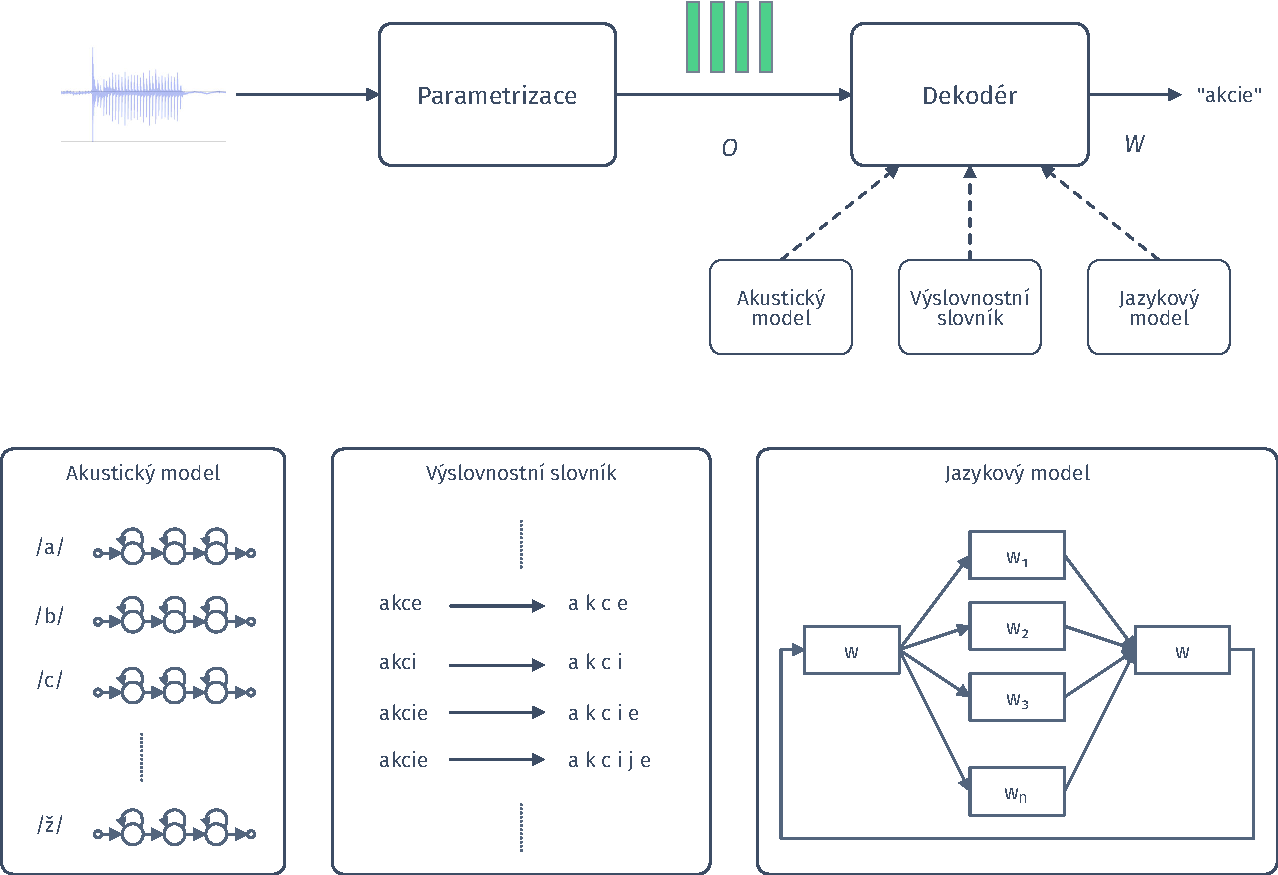
\includegraphics[width=0.9\textwidth]{./ch4-asr/img/decoding.pdf}
  \caption[Schéma ASR systému pracující se statistickou.]{Schéma automatického systému rozpoznávání řeči pracující na statistickém přístupu.}
  \label{fig:asr:decoding}
\end{figure}

\begin{equation}
  \hat{W} = \argmax_W\ P\left(W | \boldsymbol{O}\right).
  \label{eq:asr:decoding}
\end{equation}

\newpage Pomocí Bayesova pravidla je možné podmíněnou pravděpodobnost $P\left(W | \boldsymbol{O}\right)$ vyjádřit jako

\begin{equation}
  P\left(W | \boldsymbol{O}\right) = \frac{P(\boldsymbol{O}|W)P(W)}{P(\boldsymbol{O})},
\end{equation}

\noindent kde podmíněná pravděpodobnost $P(\boldsymbol{O} | W)$ odhaduje sekvenci pozorování $\boldsymbol{O}$ za předpokladu výskytu posloupnosti slov $W$. Tento výpočet je realizován \textbf{akustický modelem} (viz obr. \ref{fig:asr:decoding}). K určení $\hat{W}$ je ještě nezbytné znát pravděpodobnost výskytu požadované posloupnosti slov $P\left(W\right)$, o stanovení této pravděpodobnosti se stará \textbf{jazykový model}. Jelikož pravděpodobnost $P(\boldsymbol{O})$ je z principu nezávislá na sekvenci slov $W$, je možné rovnici (\ref{eq:asr:decoding}) upravit do tvaru

\begin{equation}
  \hat{W} = \argmax_W\ P\left(\boldsymbol{O} | W\right)P(W).
  \label{eq:asr:decoding:generic}
\end{equation}

Takto upravená rovnice představuje obecné pravidlo dekódování a její členy reprezentují základní stavební prvky ASR systému. Pro doplnění je nutné dodat, že \textbf{slovník} obsahuje seznam všech slov, se kterými je systém schopen pracovat. Tento seznam jobsahuje rovněž jejich fonetickou transkripci. Všechny tyto části jsou součástí \textbf{dekodéru}, který realizuje prohledávací strategii. V následujícím textu budou jednotlivé stavební prvky ASR systému popsány podrobněji.

% !TEX root = ../thesis.tex
\section{Parametrizace řečového signálu}
\label{chap:asr:parametrization}

Stejně jako v mnoha jiných odvětvích, i při rozpoznávání řeči je v mnoha případech inspirací člověk. Pro získání sekvence pozorování (příznaků) vycházíme z \textbf{modelování produkce řeči} a \textbf{modelování procesu slyšení}.

\subsection{Modelování produkce řeči}
\label{chap:asr:parametrization:production}

Cílem modelování produkce řeči je nalezení matematických vztahů, které poslouží k~reprezentaci fyzikálních dějů spojených s produkcí řeči. Základem je parametrizační technika \textbf{lineárního prediktivního kódování}, známá pod anglickou zkratkou LPC\footnote{Linear Predictive Coding} \cite{Benesty2007}. Vychází z představy, že hlasové ústrojí člověka je schopno vytvářet tři různé typy řečových zvuků:

\begin{itemize}
  \item \textit{samohlásky} - ty se řadí mezi znělé typy zvuků produkované periodickým buzením vznikajícím pulsy vzduchu, které jsou produkovány hlasivkami;
  \item \textit{frikativy} (např. $/f/$\footnote{Zápis $/f/$ symbolizuje foném, což je akustická reprezentace písmene, \textit{f}. Konkrétní zápisy se mohou lišit podle použité fonetické abecedy. V Čechách se nejčastěji používá abeceda $SAMPA$ či $Z\check{C}FA$.}) - někdy nazývané jako třené souhlásky, protože vznikají třením vydechovaného proudu vzduchu o překážku, kterou mouhou být například zuby nebo jazyk, v některém místě hlasového ústrojí;
  \item \textit{explozivy} (např. $/b/$, $/p/$ ap.) - také nazývané jako souhlásky výbuchové, se tvoří úplným uzavřením vydechovaného proudu vzduchu pomocí artikulačních orgánů. To se následně projeví jako krátká pauza (tzv. okluze), po které následuje náhlé jednorázové uvolnění a únik nahromaděného vzduchu (tzv. exploze) \cite{Psutka2006}.
\end{itemize}

Snahou je navrhnout takový model hlasového traktu, který bude dobře popisovat výše zmíněné řečové zvuky. Nesmí se však zapomenout na možnou přílišnou složitost~a nedostatečnou přesnost modelu. Jako ideální se může jevit lineárně časově invariantní model. Bohužel lidskou řeč lze klasifikovat jako kontinuální časově variantní a v~některých situacích dokonce nelineární proces, proto je téměř nemožné jej přesně namodelovat. Pokud však budeme předpokládat, že v konkrétním krátkém časovém úseku zůstává buzení a parametry hlasivkového traktu přibližně konstantní, tak je možné navrhnout lineární časově invariantní model řeči, který je platný pro krátké časové úseky. Tuto podmínku lze považovat za platnou pro intervaly délky od $10$ do $30\ ms$. Odtud také vychází uvažovaná perioda segmentů řeči, zmíněná v úvodu této kapitoly. Pro tyto segmenty je pak možné proces vytváření řeči modelovat pomocí tzv. \textbf{krátkodobého modelu}, který má v krátkých časových intervalech pevné parametry \cite{Holmes2001}.

Odvození obecného diskrétního modelu hlasivkového traktu je založeno na zjednodušeném modelu produkce řeči, jehož struktura je ukázána na obr. \ref{fig:asr:model:speech}. Ten je tvořen třemi dílčími částmi, konkrétně modelem hlasivek, modelem hlasivkového traktu a modelem vyzařovaného zvuku. K odvození a popisu vlastností modelu se využívá výhod Z-transformace \cite{Psutka2006}.

\begin{figure}[hbpt]
  \centering
  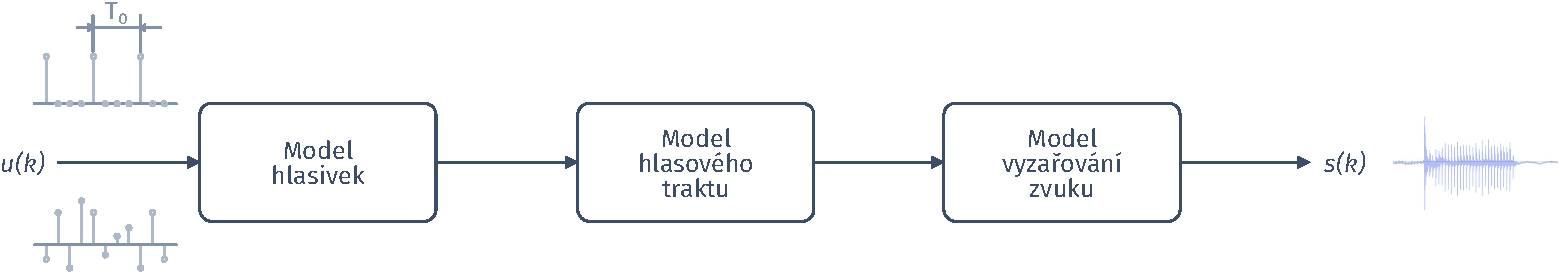
\includegraphics[width=0.9\textwidth]{./ch4-asr/img/speech_model.pdf}
  \caption{Blokové schéma modelu produkce řeči.}
  \label{fig:asr:model:speech}
\end{figure}


Krátkodobý model produkce řeči lze aproximovat celopólovým modelem charakteru filtru $H(z)$ ve tvaru

\begin{equation}
  H(z) = \frac{G}{1 + \sum_{i = 1}^{Q} a_{i} z^{-i}} = \frac{G}{A(z)},
  \label{eq:asr:lpc:generic}
\end{equation}

\noindent kde $G$ představuje celkové zesílení, $Q$ je řád modelu a $a_i$ jsou parametry modelu. Vstupem modelu je buzení $u(k)$ (viz obr. \ref{fig:asr:model:speech}), které je v případě znělých zvuků reprezentováno sledem pulsů s periodou $T_0$\footnote{Perioda základního hlasivkového tónu.} a pro neznělé zvuky je tvořeno náhodným šumem s plochým spektrem. V časové oblasti je pak diskrétní výstupní odezva při fixovaných parametrech hlasového traktu ($10 - 30\ ms$) dána konvolucí buzení a impulzní odezvy krátkodobého modelu. Na základě toho je možné model upravit do podoby znázorněné na obr. \ref{fig:asr:model:speech:excitation}, kde $u(k)$ je buzení a $s(k)$ je výstupní signál s parametry hlasového ústrojí odpovídajícími parametrům $a_i$ celopólového modelu.

\begin{figure}[hbpt]
  \centering
  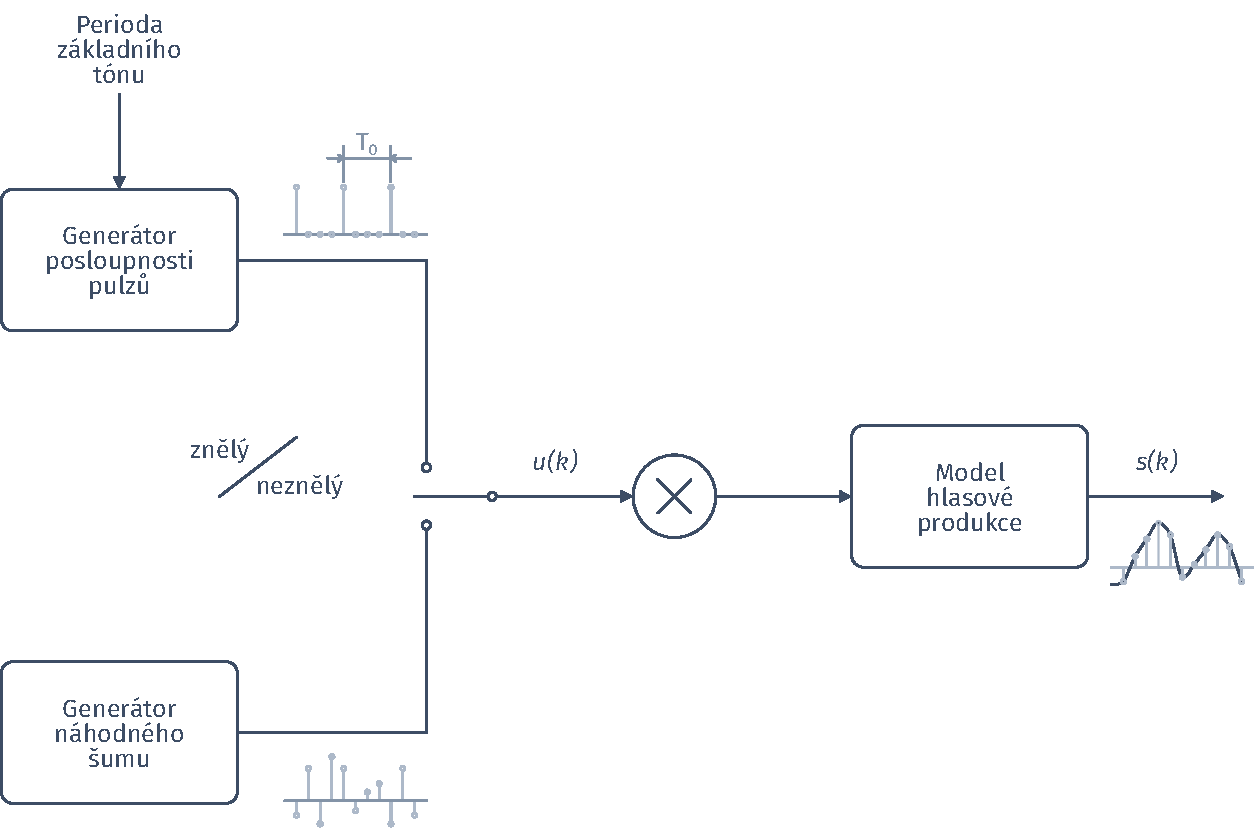
\includegraphics[width=0.9\textwidth]{./ch4-asr/img/speech_process.pdf}
  \caption{Blokové schéma upraveného modelu produkce řeči.}
  \label{fig:asr:model:speech:excitation}
\end{figure}

K odhadu parametrů $a_i$ slouží \textbf{lineární prediktivní analýza}. Odhad probíhá přímo z krátkodobého řečového signálu. Přenosové vlastnosti krátkodobého modelu je možné popsat rovnicí (\ref{eq:asr:lpc:generic}). Myšlenka metody LPC vychází z předpokladu, že vzorek $k$ řečového signálu je možné popsat lineární kombinací $Q$ předchozích vzorků a buzení $u(k)$, což lze matematicky vyjádřit pomocí následující rovnice ve tvaru

\begin{equation}
  s(k) = - \sum_{i = 1}^{Q} a_i s(k-1) + Gu(k).
  \label{eq:asr:lpc:generic:edited}
\end{equation}

\noindent %Z rovnice (\ref{eq:asr:lpc:generic:edited}) 
Je patrné, že se LPC snaží odhadnout parametry modelu $a_i$ a zesílení $G$ pomocí známé reálně naměřené posloupnosti vzorků řeči $s(k)$. K odhadu se používá principu minimalizace kvadratické chyby krátkodobé energie signálu $e\left(k\right)$. Ta je v časové oblasti popsána vztahem

\begin{equation}
  E = \sum_{k} e^2(k) = \sum_{k} \left[ s(k) - s'(k)\right]^2 = \sum_{k} \left( s(k) + \sum_{i = 1}^{Q} a_i s(k-1) + Gu(k) \right),
\end{equation}

\noindent kde $s(k)$ jsou vzorky reálného řečového signálu a $s'(k)$ jsou ty predikované LPC filtrem. Pro nalezení minimální hodnoty krátkodobé chyby predikce $E$ pro konkrétní analyzovaný segment, je použita metoda nejmenších čtverců. K výpočtu konkrétních koeficientů modelu $a_i$ je možné použít rekurzivního Durbinova algoritmu \cite{Holmes2001}.

Další možností jak modelovat hlasový trakt je využít popis pomocí \textbf{kepstrálních koeficientů lineární predikce} $c\left(k\right)$. Kepstrum k-tého mikrosegmentu řečového signálu $s\left(k\right)$ je definováno vztahem % (\ref{eq:asr:lpc:cepstrum:generic}), 


\begin{equation}
  c(k) = \mathcal{F}^{-1}\left\{\log\left| \mathcal{F}\left\{s(k)\right\} \right|\right\}.
  \label{eq:asr:lpc:cepstrum:generic}
\end{equation}

\noindent kde $\mathcal{F}$ představuje operátor diskrétní Fourierovy transformace (DFT) a $\mathcal{F}^{-1}$ reprezentuje inverzní diskrétní Fourierovy transformace (IDFT). Postup výpočtu je znázorněn na obr. \ref{fig:asr:model:speech:cepstrum}.

\begin{figure}[hbpt]
  \centering
  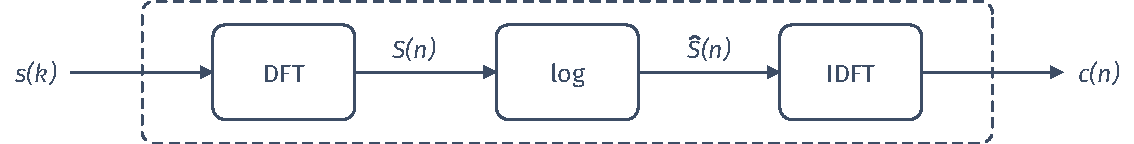
\includegraphics[width=0.9\textwidth]{./ch4-asr/img/cepstrum.pdf}
  \caption{Blokové schéma principu výpočtu kepstra.}
  \label{fig:asr:model:speech:cepstrum}
\end{figure}

Pro získání kepstrálních koeficientů lineární predikce lze využít vztah (\ref{eq:asr:lpc:generic}), který po zlogaritmování přejde do tvaru

\begin{equation}
  \log H(z) = \log \left( \frac{G}{A(z)} \right).
  \label{eq:asr:lpc:cepstrum}
\end{equation}

\noindent Člen $A(z)$ je polynomem proměnné $z^{-1}$ řádu $Q$. Pokud všechny jeho kořeny leží uvnitř jednotkové kružnice, tak lze aplikovat Taylorův rozvoj a vztah (\ref{eq:asr:lpc:cepstrum}), tedy lze zapsat jako

\begin{equation}
  \log \left( \frac{G}{A(z)} \right) = c(0) + c(1)z^{-1} + \dots = \sum_{k=0}^{\infty} c(k)z^{-k},
  \label{eq:asr:lpc:cepstrum:taylor}
\end{equation}

\noindent kde $c(k)$ jsou tzv. kepstrální koeficienty LPC. Po zderivování obou stran rovnice přejde vztah (\ref{eq:asr:lpc:cepstrum:taylor}) do tvaru

\begin{equation}
  - \sum_{i=1}^{Q} ia_iz^{-i} = \left( \sum_{k=0}^{\infty} kc(k)z^{-k} \right)\left( \sum_{i=0}^{Q} a_iz^{-i}\right).
  \label{eq:asr:lpc:cepstrum:deriv}
\end{equation}

\noindent Jestliže se $a_i = 1$, pak lze po roznásobení pravé strany rovnice (\ref{eq:asr:lpc:cepstrum:deriv}) a po následném porovnání členů u stejných mocnin proměnné $z$ zapsat vztahy pro výpočet kepstrálních koeficientů LPC ve tvaru

\begin{align}
  \begin{split}
    c(1) &= -a_1, \\
    c(k) &=
    \begin{cases}
      - a_k - \sum_{i=1}^{k-1} \left(\frac{i}{k}\right) c(i) a_{k-1},  & \quad \text{pro } 2 \leq k \leq Q, \\
      - \sum_{i=1}^{Q} \left(\frac{k - i}{k}\right) c(k-i) a_i,  & \quad \text{pro } k = Q + 1, Q + 2, \dots \quad ,
    \end{cases}
  \end{split}
  \label{eq:asr:lpc:cepstrum:coef}
\end{align}

\noindent kde $k = 1, 2, \dots , Q^{*}$. $Q^{*}$ je počet kepstrálních koeficientů pro které musí platit $Q^{*} \geq Q$. Kepstrální koeficienty LPC jsou vztaženy ke spektrální obálce mikrosegmentu řeči odvozené LPC analýzou. 

Spektrální obálku je následně možné získat z rovnice (\ref{eq:asr:lpc:generic}) dosazením $z = e^{j\omega}$. Pro uspokojivou reprezentaci se tradičně volí $Q$ v rozmezí $7-15$ v závislosti na spektrální šířce přenášeného pásma a požadované přesnosti aproximace. Z toho plyne, že pro popis mikrosegmentu řeči by mohl být dostačující příznakový vektor o $15$ koeficientech.

\subsection{Modelování procesu slyšení}
\label{chap:asr:parametrization:hearing}

Zvuk představuje mechanické vlnění hmotných částic, které se šíří v plynném, kapaném nebo tuhém prostředí. Z fyziologického pohledu je však zvuk považován pouze za slyšitelné vlnění. To je takové, které je schopno vnímat sluchové ústrojí člověka. Zpravidla se jedná o frekvence $16\ Hz - 20\ kHz$. Pro každého člověka je ale toto rozmezí individuální a mění se s věkem. S přibývajícím věkem a sluchovou zátěží klesá hlavně horní mezní kmitočet \cite{Psutka2006}.

To, zda je člověk schopen daný zvuk slyšet, však není závislé pouze na frekvenci zvuku. Velmi podstatná je i intenzita zvuku, která se rovná energii zvukového vlnění, která projde za jednotku času jednotkovou plochou kolmou ke směru šíření vln. Zároveň je úměrná akustickému tlaku zvukové vlny, tj. tlaku, kterým zvukové vlny působí na nějakou překážku. V případě člověka lze překážkou chápat ušní bubínek. Závislost mezi intenzitou zvuku $I\ \left[Wm^{-2}\right]$ a akustickým tlakem $p\ \left[Pa\right]$ je vyjádřen vztahem

\begin{equation}
  I = \frac{p^{2}}{z},
  \label{eq:asr:mfcc:intesity}
\end{equation}

\noindent kde $z$ je měrná akustická impedance prostředí, kterým se zvuk šíří. Lidské ucho je schopno vnímat akustický tlak v rozsahu od $2\cdot10^{-5}$ až $2\cdot10^{2}\ Pa$, tj. v rozsahu sedmi řádů. Z praktického důvodu se tedy používá logaritmické stupnice. K vyjadřování pak slouží logaritmus poměru uvažované veličiny a mezinárodně normované referenční hodnoty téže veličiny \cite{Psutka2006}. Hladina intenzity $L_{I}$ je pak definována vztahem

\begin{equation}
  L_{I} = 10\log_{10}\frac{I}{I_{0}},
  \label{eq:asr:mfcc:intesity:level}
\end{equation}

\noindent kde $I$ představuje intenzitu zvuku a $I_{0} = 10^{-12}\ Wm^{-2}$ referenční hodnotu intenzity. Pro hladinu akustického tlaku platí

\begin{equation}
  L_{p} = 20\log_{10}\frac{p}{p_{0}},
  \label{eq:asr:mfcc:pressure:level}
\end{equation}

\noindent kde $p$ je akustický tlak a $p_{0} = 2\cdot10^{-5}\ Pa$ je referenční hodnota akustického tlaku. Hodnoty veličin $L_{I}$ a $L_{p}$ jsou obvykle udávány v decibelech. %$\left[dB\right]$.

Důležitým pojmem je pak \textbf{práh slyšitelnosti}, který představuje minimální intenzitu zvuku potřebnou k tomu, aby jej šlověk mohl slyšet, viz obr. \ref{fig:asr:mfcc:acoustic:characteristic}. Tento práh je zcela subjektivní a je závislý na frekvenci. Obecně je lidský sluch nejcitlivější na frekvence $3 - 4\ kHz$. Směrem k nižším i vyšším kmitočtům citlivost sluchu klesá. \textbf{Práh bolesti} představuje horní mez intenzity sluchového pole (viz obr. \ref{fig:asr:mfcc:acoustic:characteristic}), při níž již posluchač pociťuje bolest. Překročení této meze může vést k poškození sluchu \cite{Holmes2001}.

\begin{figure}[hbpt]
  \centering
  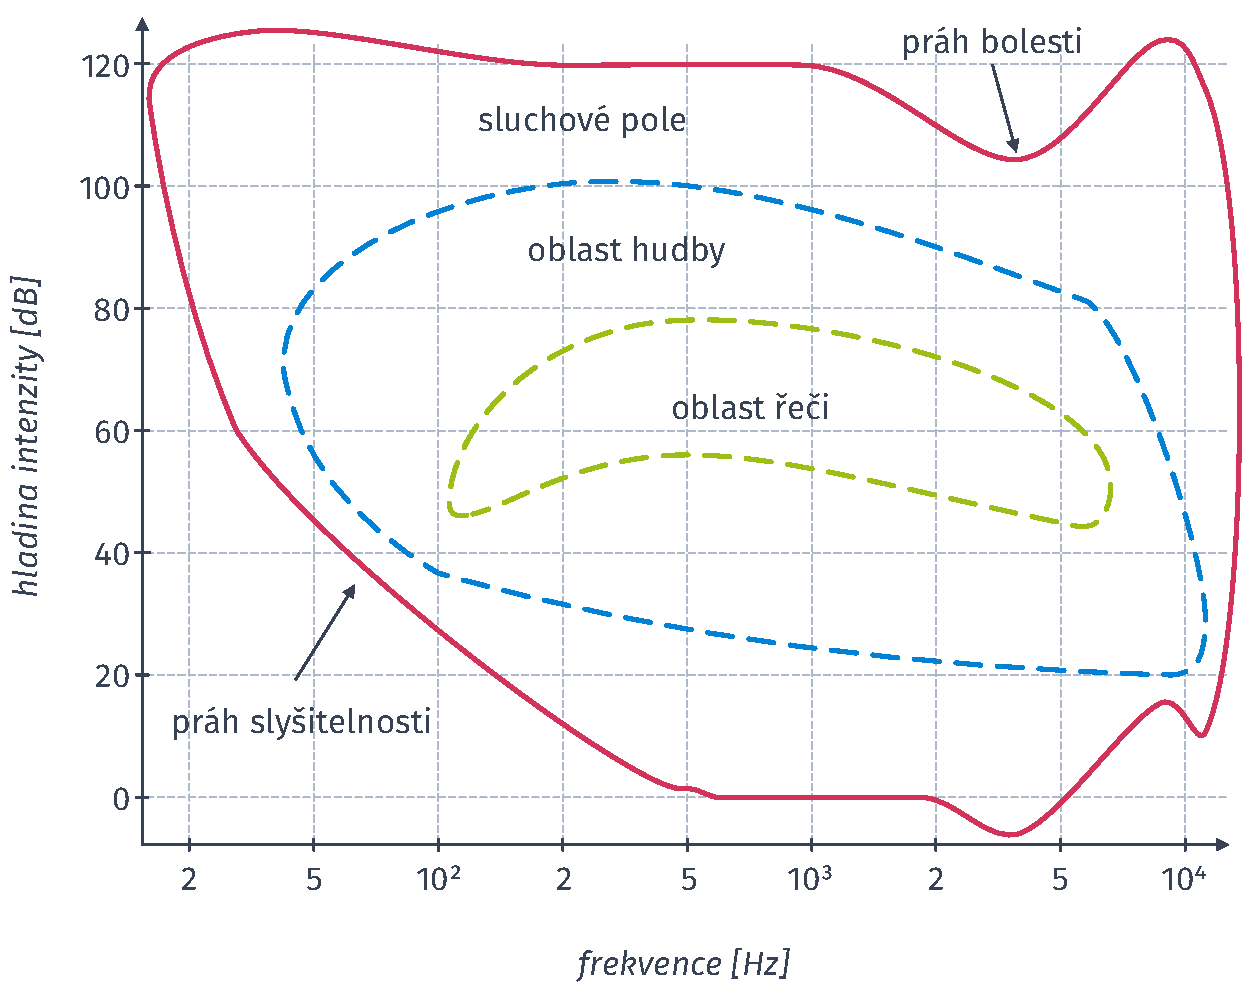
\includegraphics[width=0.75\textwidth]{./ch4-asr/img/listening_perception.pdf}
  \caption[Charakteristické oblasti vnímání akustického signálu.]{Charakteristické oblasti vnímání akustického signálu lidským sluchem. $L_p = 20log(p/p0),\ p0 = 2\bullet10^{–5}\ Pa$.}
  \label{fig:asr:mfcc:acoustic:characteristic}
\end{figure}

Hlasitost zvuku je závislost intenzity na frekvenci a je zcela subjektivní pocit, kterým člověk posuzuje intenzitu daného zvuku. Na obr. \ref{fig:asr:mfcc:acoustic:levels} jsou vyznačeny hladiny hlasitosti, které vznikly spojením bodů ve sluchovém poli (obr. \ref{fig:asr:mfcc:acoustic:characteristic}), odpovídající tónům, které člověk vnímá stejně hlasitě. Z křivek je patrné, že subjektivní hlasitost se mění s frekvencí zvuku. Zvuky s nižší frekvencí vnímáme méně hlasitěji než zvuky s vyšší frekvencí, zejména pak zvuky v rozmezí $3 - 4\ kHz$ \cite{Psutka2006}.

\begin{figure}[hbpt]
  \centering
  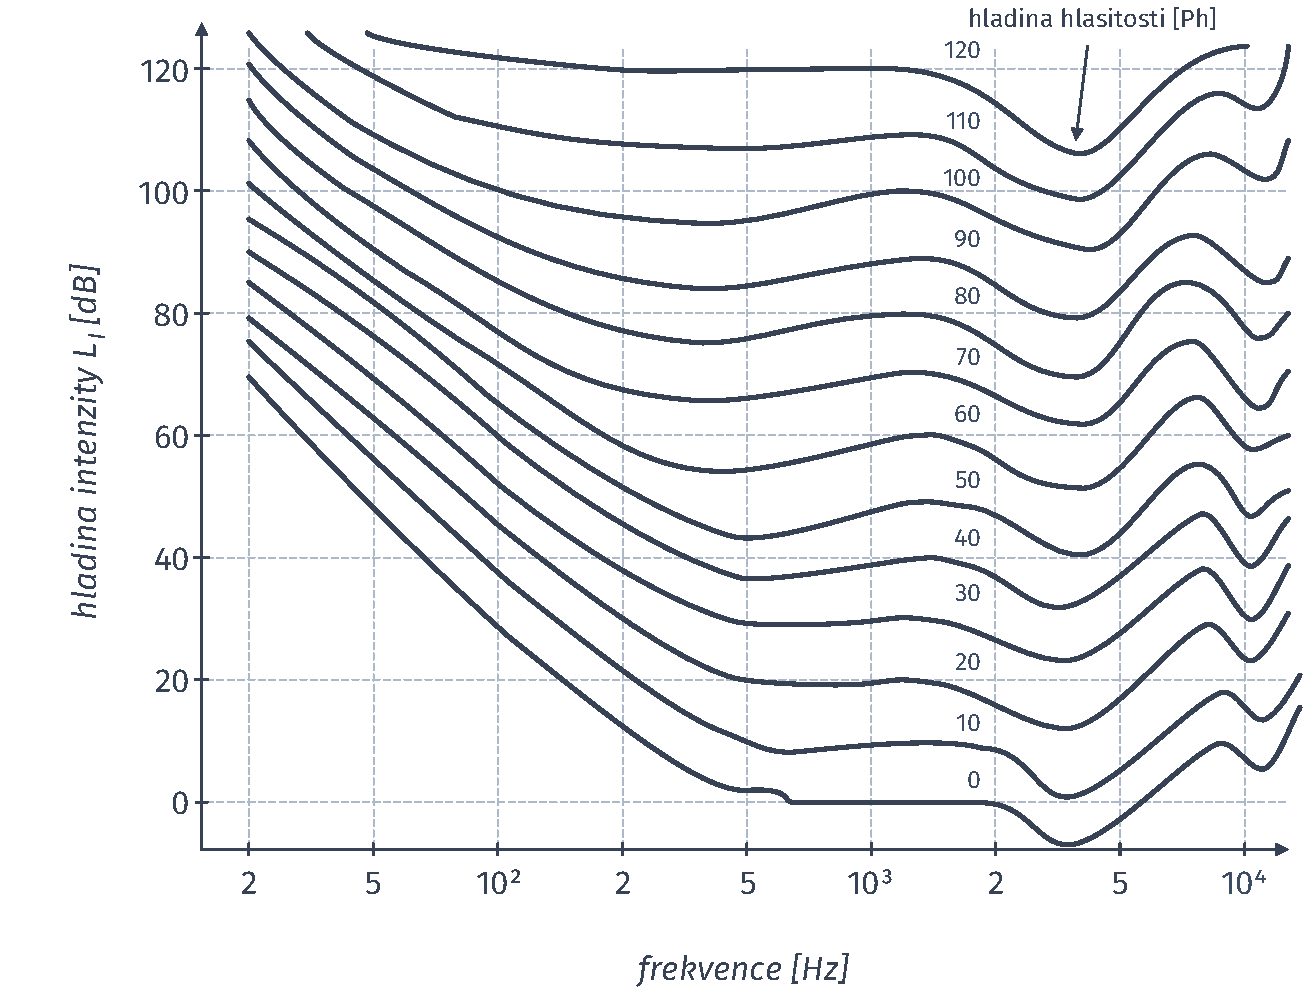
\includegraphics[width=0.75\textwidth]{./ch4-asr/img/listening_levels.pdf}
  \caption[Křívky stejné hlasitosti.]{Křivky stejné hlasitosti. $L_p = 20log(p/p0),\ p0 = 2\bullet10^{–5}\ Pa$.}
  \label{fig:asr:mfcc:acoustic:levels}
\end{figure}

Principem modelování procesu slyšení je postižení kompenzace nelineárního vnímání frekvencí lidským sluchem a respektování maskování zvuků včetně tzv. kritických pásem slyšení. Maskování zvuků je přirozená vlastnost lidského sluchu. Rozumí se jím jev, kdy je vnímání jednoho zvuku ovlivněno přítomností jiného zvuku. Jinými slovy lze říci, že přítomnost jednoho zvuku zvyšuje práh slyšitelnosti pro jiný zvuk. Ten buď zní současně nebo s drobným časovým odstupem od toho prvního. Tento jev je jakýsi \uv{psychologický filtr}, který ignoruje veškerý šum ležící mimo určité kritické pásmo slyšení. Šířka kritického pásma je přitom závislá na frekvenci poslouchaného tónu. Často užívanými metodami pro modelování procesu slyšení jsou \textbf{melovská kepstrální filtrace} a \textbf{perceptivní lineární prediktivní analýza}.

\subsubsection{Melovské kepstrální koeficienty}

Metoda melovských frekvenčních kepstrálních koeficientů (MFCC) se snaží respektovat výše zmíněné vlastnosti lidského sluchu, především se snaží dodržet kritická pásma slyšení a vliv subjektivního vnímání výšky tónů.

Základem MFCC je využití banky filtrů a lineárního rozložení frekvencí v tzv. \textbf{melovské frekvenční škále} definované vztahem

\begin{equation}
  f_m = 2595 \log \left(1 + \frac{f}{700}\right),
  \label{eq:asr:mfcc:melscale}
\end{equation}

\noindent kde $f \left[Hz\right]$ je frekvence v lineární škále a $f_m \left[mel\right]$ je odpovídající frekvence v melovské stupnici. Melovský filtr má trojúhelníkový tvar. Banka obsahuje $M^{*}$ filtrů rozmístěných lineárně v melovských frekvenčních souřadnicích, a to tak, že dva sousední filtry se navzájem o polovinu překrývají. Pro střední frekvence jednotlivých filtrů $b_{m,i}$ v melovské škále platí vztah

\begin{equation}
  b_{m,i} = b_{m,i-1} + \Delta_{m},
  \label{eq:asr:mfcc:freq}
\end{equation}

\noindent kde $b_{m, 0} = 0\ mel$, $i = 1, 2,\ \dots\ , M^{*}$, a $\Delta_m = B_{m,w} / (M^{*} + 1)$, kde $B_{m,w}$ je celková šířka pásma v melovské škále. Ukázka banky filtrů v této škále je znázorněna na obr. \ref{fig:asr:mfcc:bank:mel}. Pro výpočet odezvy filtrů je však nezbytné přepočítat všechny koeficienty FFT do melovské frekvenční škály.

\begin{figure}[hbpt]
  \centering
  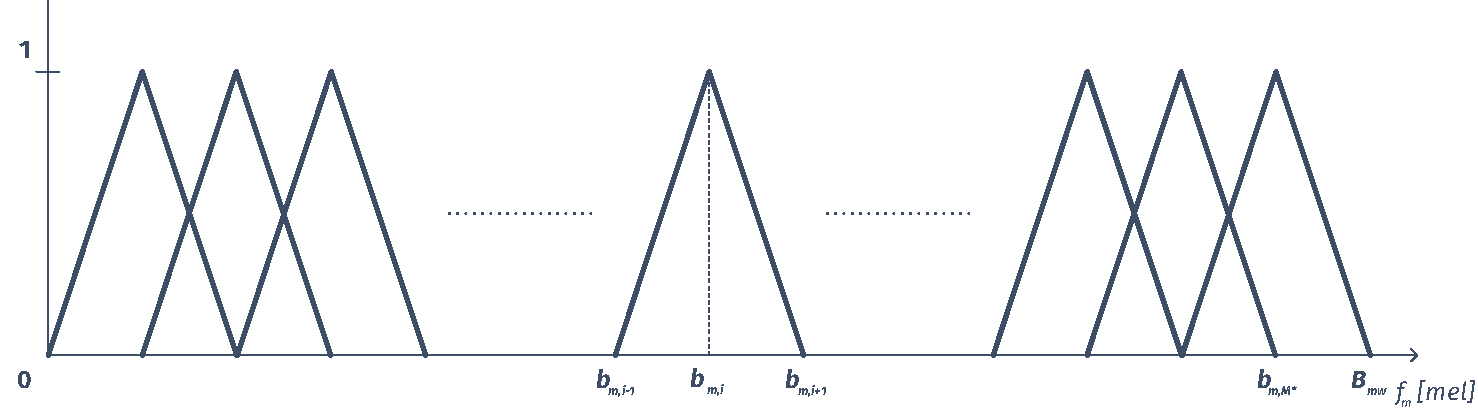
\includegraphics[width=0.9\textwidth]{./ch4-asr/img/filter_bank-mel.pdf}
  \caption{Rozložení banky trojúhelníkových filtrů v melovské frekvenční škále.}
  \label{fig:asr:mfcc:bank:mel}
\end{figure}

\noindent Vhodnější je vyjádření trojúhelníkových filtrů ve frekvenční škále s měřítkem v herzích. K přepočtu středních frekvencí $b_{m,i}$ se využívá inverzního vztahu k (\ref{eq:asr:mfcc:melscale}), tedy

\begin{equation}
  f = 700 \left[ \exp\left( 0,887.10^{-3} f_m \right) - 1 \right].
  \label{eq:asr:mfcc:melscale:inverse}
\end{equation}

\noindent Střední frekvence $b_i$ jednotlivých filtrů jsou vyjádřené také v herzích. Na rozdíl od popisu v melovské škále jsou filtry rozmístěny nelineárně napříč celým analyzovaným spektrem, viz obr. \ref{fig:asr:mfcc:bank:hz}.

\begin{figure}[hbpt]
  \centering
  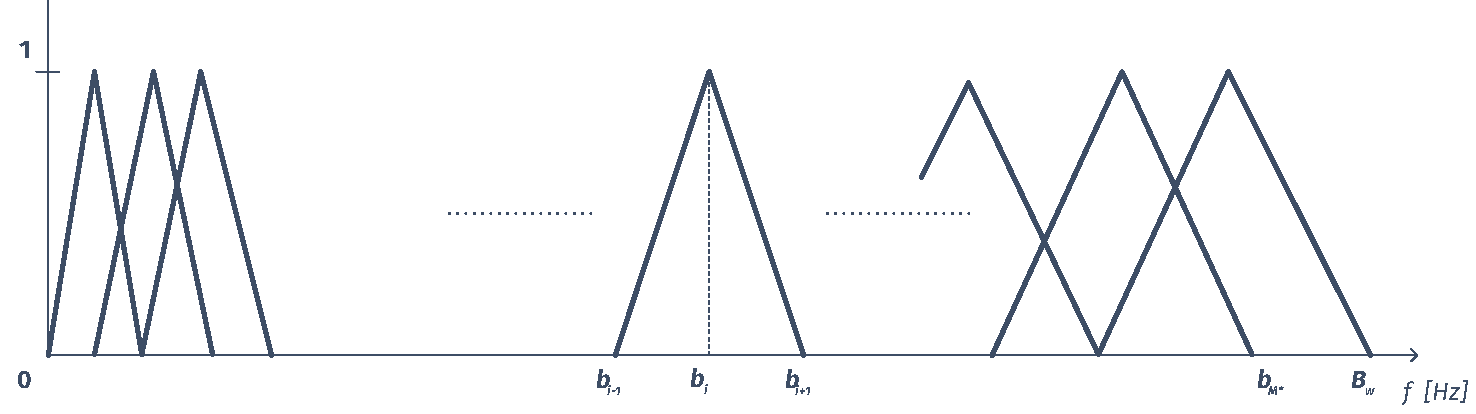
\includegraphics[width=0.9\textwidth]{./ch4-asr/img/filter_bank-hz.pdf}
  \caption{Rozložení banky trojúhelníkových filtrů ve frekvenční škále.}
  \label{fig:asr:mfcc:bank:hz}
\end{figure}

Na vstup systému jsou postupně přivedeny mikrosegmenty řečového signálu\footnote{Jednotlivé mikrosegmenty byly nejprve předzpracovány , tj. prošly tzv. preemfází. Ta spočívá ve zdůraznění amplitud spektrálních složek řečového signálu s jejich vzrůstající frekvencí \cite{Psutka2006}.} $s\left(k\right)$ o konstantní délce a pro ně jsou určeny odpovídající koeficienty $c\left(k\right)$. Pro jednotlivé mikrosegmenty je pomocí FFT vypočteno amplitudové spektrum $\left| S(f) \right|$ a následuje klíčová část celého procesu, melovská filtrace. Odezvy filtrů ve frekvenční oblasti lze stanovit pomocí vztahu

\begin{equation}
  y_m(i) = \sum_{f=b_{i-1}}^{b_{i+1}} \left| S(f) \right| u\left(f, i\right),  \quad i = 1, 2,\ \dots\ ,M^{*},
  \label{eq:asr:mfcc:freq:responce}
\end{equation}

\noindent kde frekvence $f$ jsou vybírány ze souboru frekvencí využívaných při FFT výpočtu a $u(f, i)$ je vyjádření konkrétního trojúhelníkového filtru $i$. Průchod filtrem tedy znamená, že každý koeficient FFT je násoben odpovídajícím ziskem filtru a výsledky jsou pro příslušné filtry akumulovány. Logaritmováním akumulovaných koeficientů $y_{m}(i)$ je realizován převod do kepstrální oblasti. Tento krok příznivě omezí dynamiku signálu \cite{Benesty2007}. Posledním krokem při výpočtu melovských kepstrálních koeficientů $\left\{c_m\left(j\right)\right\}_{j=1}^{M}$ je provedení IDFT podle vztahu (\ref{eq:asr:lpc:cepstrum:generic}). V případě MFCC se ale používá diskrétní kosinová transformace (DCT), protože spektrum je reálné a symetrické. K výpočtu slouží vztah

\begin{equation}
  c_{m}(j) = \sum_{i=1}^{M^{*}} \log y_m(i) \cos\left( \frac{\pi j}{M^{*}}\left(i - 0,5\right) \right) \quad \text{pro}\ j = 0, 1,\ \dots\ ,M,
  \label{eq:asr:mfcc:coef}
\end{equation}

\noindent kde $M^{*}$ je počet pásem melovkého pásmového filtru a $M$ je počet melovských kepstrálních koeficientů. Počet těchto koeficientů $M$ se volí podstatně menší než je počet pásem melovského pásmového filtru $M^{*}$, obvykle se uvažuje prvních $10\ \text{až}\ 13$ koeficientů. Velmi často se také používá $1.$ a $2.$ z těchto koeficientů, protože svým způsobem zohledňují dynamickou složku řeči.

\subsubsection{Perceptivní lineární prediktivní analýza}

Stejně jako MFCC, tak také i \textbf{perceptivní lineární prediktivní analýza (PLP)} vychází z lidského vnímání a slyšení zvuků. Snaha je postihnout z psychofyziky slyšení zejména kritická pásma spektrální citlivosti, vztah mezi intenzitou a vnímáním hlasitosti a také křivky stejné hlasitosti \cite{Psutka2006}. PLP podobně jako LPC pak aproximuje získané sluchové spektrum koeficienty autoregresního celopólového modelu.

Prvním krokem PLP analýzy je \textbf{výpočet výkonového spektra řečového signálu}. Pro konkrétní předzpracovaný\footnote{Ještě před výpočtem je stejně jako u MFCC aplikována preemfáze.} mikrosegment řečového signálu $s(k)$ aplikujeme DFT. Krátkodobé spektrum je pak definováno vztahem

\begin{equation}
  P\left(\omega\right) = \left| S\left(\omega\right) \right|^{2} = \left[Re\ S\left(\omega\right)\right]^2 + \left[Im\ S\left( \omega \right) \right]^2.
  \label{eq:asr:plp:spectr}
\end{equation}

\noindent Poté následuje kompenzace nelineárního vnímání změn ve výšce zvuku. Vnímání je logaritmické, proto je nutné provést nelineární transformaci frekvenční osy pomocí vzorce

\begin{equation}
  \Omega\left(\omega\right) = 6 \ln \left( \frac{\omega}{1200\pi} + \sqrt{\left(\frac{\omega}{1200\pi}\right)^2 + 1} \right),
  \label{eq:asr:plp:transform}
\end{equation}

\noindent kde $\omega = 2\pi f\ \left[rad/s\right]$ a $\Omega\left(\omega\right)\ \left[Bark\right]$.

Zahrnutí kritických pásem slyšení (tzv. maskování zvuku) je realizováno navržením vhodného filtru typu pásmová propust šířky jednoho kritického pásma. Stejně jako v případě MFCC se jedná o banku filtrů, kde na sebe jednotlivé filtry ve frekvenční oblasti navazují.
%Na Barkově frekvenční ose (viz (\ref{eq:asr:plp:transform})) mají všechny filtry šířku $1$ a jsou lineárně rozmístěny.
Na obr. \ref{fig:asr:plp:filter} je zobrazen průběh jednoho takového filtru. Filtr má strmost $+20\ dB/Bark$ směrem k nižším frekvencím a $-50\ dB/Bark$ směrem k vyšším frekvencím.

\begin{figure}[hbpt]
  \centering
  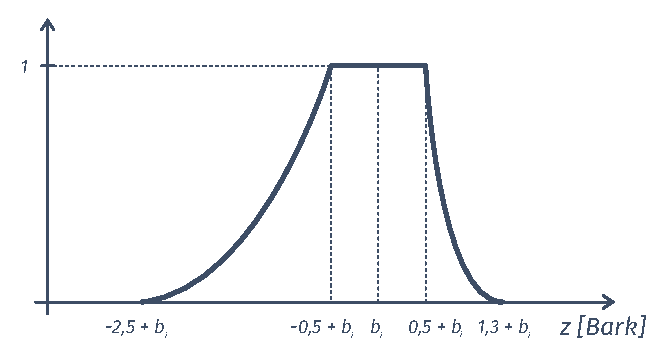
\includegraphics[width=0.5\textwidth]{./ch4-asr/img/plp_filter.pdf}
  \caption{Ukázka filtru umístěného na Barkově frekvenční ose.}
  \label{fig:asr:plp:filter}
\end{figure}

\newpage \noindent Na Barkově frekvenční ose mají jednotlivé filtry šířku $1$ a jsou podél ní lineárně rozmístěny viz obr. \ref{fig:asr:plp:bank},
% Rozmístění filtrů na Barkově frekvenční ose je pak znázorněno na obr. \ref{fig:asr:plp:bank}.

\begin{figure}[hbpt]
  \centering
  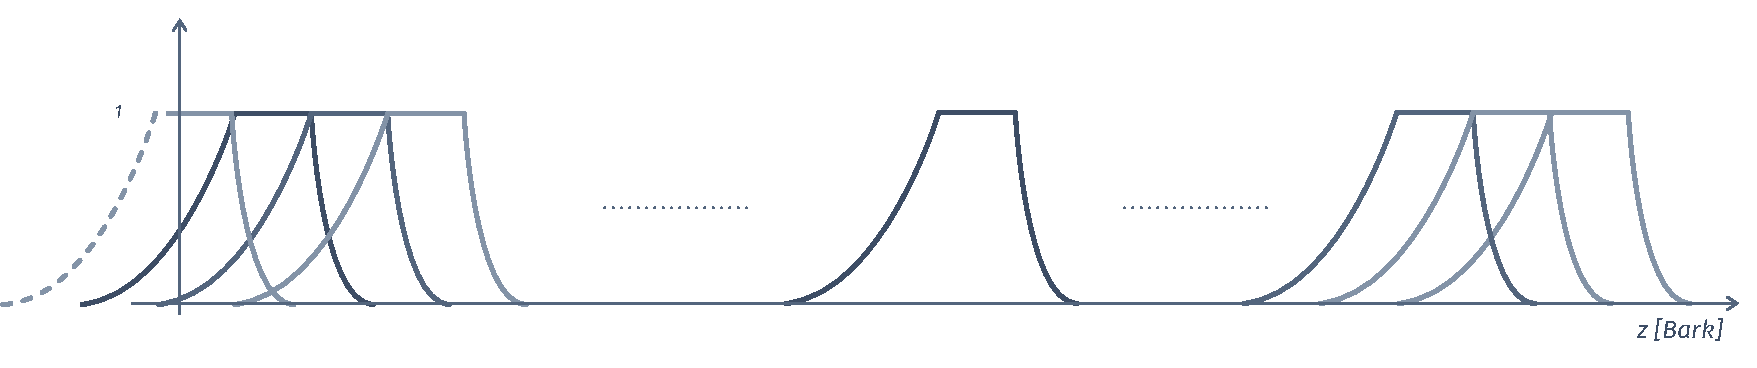
\includegraphics[width=0.9\textwidth]{./ch4-asr/img/plp-bank.pdf}
  \caption{Rozmístění filtrů na Barkově frekvenční ose.}
  \label{fig:asr:plp:bank}
\end{figure}

Jelikož člověk vnímá intenzitu zvuku v závislosti na frekvenci, tak je potřeba provést \textbf{přizpůsobení křivkám stejné hlasitosti}. Na začátku je důležité definovat referenční hlasitost, tj. hlasitost, na kterou bude normalizována. Obvykle se volí $40\ Ph$ \cite{Psutka2006}, což přibližně odpovídá hlasitosti běžné řeči. K normalizaci je použit inverzní filtr popsaný vztahem

\begin{equation}
  E\left(\omega\right) = K \frac{\omega^4\left(\omega^2 + 56,9 \cdot 10^6\right)}{\left(\omega^2 + 6,3 \cdot 10^6\right)^2\left(\omega^2 + 379,4 \cdot 10^6\right)\left(\omega^6 + 9,6 \cdot 10^{26}\right)},
  \label{eq:asr:plp:filter}
\end{equation}

\noindent kde $\omega = 2\pi f$ a $K$ je konstanta nastavená podle požadovaného zesílení. Přizpůsobení křivce stejné hlasitosti je pak možné například přenásobením celého výkonového spektra mikrosegmentů podle vztahu

\begin{equation}
  P'\left(\omega\right) = E\left(\omega\right)P\left(\omega\right),
  \label{eq:asr:plp:filter:application1}
\end{equation}

\noindent kde $P'\left(\omega\right)$ je spektrum transformované na stejnou hlasitost. Případně lze upravit tvar jednotlivých filtrů pomocí vztahu

\begin{equation}
  \Phi\left(\omega, i\right) = E\left(\omega\right)\Psi\left(\omega - \omega_i, i\right),
  \label{eq:asr:plp:filter:application2}
\end{equation}

\noindent kde $\Phi\left(\omega, i\right)$ je nový tvar filtru $i$ v závislosti na frekvenci $\omega$, $\Psi\left(\omega - \omega_i, i\right)$ je odezva filtru $i$ se středovou frekvencí $\omega_i$.

Po přizpůsobení následuje \textbf{výpočet energie jednotlivých filtrů}, to je obdobné jako u MFCC. Výpočet se provádí pro jednotlivé filtry a výsledky se pak sčítají. Matematicky to je zapsáno vztahem

\begin{equation}
  \zeta_m = \sum_{\Omega = \Omega_m - 2,5}^{\Omega_m + 1,3} P\left(\Omega\right)\Phi\left(\Omega, m\right), \quad\ m=1, 2,\ \dots\ M - 2,
  \label{eq:asr:plp:energy}
\end{equation}

\noindent kde $M$ je počet použitých filtrů (kritických pásem).

Dalším krokem výpočtu je uplatnění \textbf{\uv{zákona slyšení}}. Ten popisuje závislost mezi intenzitou a vnímanou hlasitostí. Na energie $\zeta_m$ je aplikována nelineární transformace vyjádřena vztahem

\begin{equation}
  \xi_m = \left(\zeta_m\right)^{0,3}, \quad\ m = 1, 2,\ \dots\ M-2,
  \label{eq:asr:plp:energy:transform}
\end{equation}

\noindent kde $M$ je opět počet filtrů. Díky této operaci dojde také k redukci proměnlivosti \uv{výstupů} kritických pásmových filtrů a výsledný hledaný celopólový model může být relativně nízkého řádu.

Finálním krokem je \textbf{aproximace celopólového modelu}. Ta vychází z výpočtu koeficientů celopólového modelu metody LPC, kde je model popsán vztahem (\ref{eq:asr:lpc:generic:edited}). Pro chybu predikce pak platí

\begin{equation}
  e\left(k\right) = \sum_{k} \left(s\left(k\right) + \sum_{i=1}^{Q} a_i s\left(k - i\right)\right).
  \label{eq:asr:plp:error}
\end{equation}

\noindent Aplikací Z-transformace a uvážením rovnice (\ref{eq:asr:lpc:generic}), je možné vztah (\ref{eq:asr:plp:error}) upravit do tvaru

\begin{equation}
  E\left(z\right) = \left[1 + \sum_{i=1}^{Q} a_i z^{-i}\right] S\left(z\right) = A\left(z\right)S\left(z\right),
  \label{eq:asr:plp:error:transform}
\end{equation}

\noindent kde $A\left(z\right)$ je inverzní filtr a $E\left(z\right)$, resp. $S\left(z\right)$ jsou získané Z-transformací $e\left(k\right)$, resp. $s\left(k\right)$. Celkovou chybu predikce je pak možné vyjádřit vztahem

\begin{equation}
  E\left(z\right) = \frac{1}{2\pi} \int_{-\pi}^{\pi} P\left(\omega\right) A\left(e^{j\omega}\right) A\left(e^{-j\omega}\right)d\omega,
  \label{eq:asr:plp:error:final}
\end{equation}

\noindent kde $P\left(\omega\right)$ je vypočtené výkonové spektrum. Podobně jako u LPC hledané řešení odpovídá hodnotám, pro něž je celková chyba autokorelační funkce $R\left(i\right)$ minimální. Pro konečný počet známých frekvencí je tato funkce definována vztahem

\begin{equation}
  R\left(i\right) = \frac{1}{N} \sum_{n=0}^{N-1} P\left(\omega_n\right) \cos\left(i\omega_n\right),
  \label{eq:asr:plp:error:solution}
\end{equation}

\noindent kde $i = 0,\ \dots\ Q$, $Q$ je řád autoregresního modelu a $N$ je počet bodů spektrální charakteristiky. Frekvence $\omega_n$ jsou ty, pro které jsou známé spektrální hodnoty. Pro dobrou aproximaci se volí $Q = 5$ \cite{Benesty2007}. \textbf{Výpočet kepstrálních koeficientů PLP} lze pak pro známé hodnoty $R\left(i\right)$, podobně jako u LPC, určit Durbinovým algoritmem. Nalezené koeficienty lze využít jako příznaky při návrhu parametrizátoru řeči
\cite{Holmes2001}.

K vytvoření parametrizátoru je možné použít libovolnou výše popsanou metodu. %metodu představenou v \ref{chap:asr:parametrization:production} a \ref{chap:asr:parametrization:hearing}. 
V současnosti ale převládají metody postavené na principu fungování lidského sluchu, protože amplifikují podstatnou informaci zakódovanou v řeči.

% !TEX root = ../thesis.tex
\section{Akustické modelování}
\label{chap:asr:acoustic}

Akustický model představuje v rovnici (\ref{eq:asr:decoding:generic}) podmíněnou pravděpodobnost $p(O|W)$. Úkolem akustického modelu je poskytnout co nejpřesnější odhad této pravděpodobnosti pro libovolnou posloupnost vektorů příznaků $O = \left\{o_1 o_2\ \dots\ o_T\right\}$. Velmi vhodným způsobem modelování řeči se ukázalo být využití tzv. \textbf{skrytých Markovových modelů (HMM)}. Ty vycházejí z principu vytváření řeči člověkem. V průběhu produkce řeči se hlasové ústrojí nachází vždy v krátkém časovém úseku nachází v jednom z konečného počtu konfiguracé. V tomto mikrosegmentu je pak hlasovým ústrojím generovám krátký signál, který zavisí na aktuální konfiguraci. Tento vyprodukovaný zvuk je metodami (popsanými v \ref{chap:asr:parametrization}) převeden na vektor příznaků $O$.

Skrytý Markovův model je model stochastického procesu. Na ten je možné nahlížet jako na pravděpodobnostní konečný automat, který v diskrétních časových okamžicích generuje náhodnou posloupnost vektorů příznaků $O = \left\{o_1 o_2\ \dots\ o_T\right\}$. Model v každém časovém kroku změní stav svůj $s_j$ podle předem daných pravděpodobností přechodu $a_{ij}$. Přechod ze stavu $s_i$ do stavu $s_j$ má za následek vygenerování výstupního vektoru pozorování $o_t$ a to podle rozdělení výstpní pravděpodobnosti $b_j\left(o_t\right)$ příslušné k tomuto stavu \cite{Psutka2006}.

Podmínění pravděpodobnost přechodu $a_{ij}$ určuje, s jakou pravděpodobností přechází model ze stavu $i$ v čase $t$, do stavu $j$ v čase $t+1$. Platí tedy

\begin{equation}
  a_{ij} = p\left(s\left(t+1\right)=s_j|s\left(t\right)=s_i\right),
  \label{eq:asr:acoustic:conditional}
\end{equation}

\noindent kde $s\left(t\right)$ je stav modelu v čase $t$. Další podmínkou je, že pro všechny stavy $i$, $i=1,2,\dots\,N$, platí

\begin{equation}
  \sum_{j=1}^{N} a_{ij} = 1.
  \label{eq:asr:acoustic:state:condition}
\end{equation}

\noindent Funkce rozdělení výstupní pravděpodobnosti $b_j\left(o_t\right)$ popisují rozdělení pravděpodobnosti pozorování $o_t$ produkovaného ve stavu $s_j$ v čase $t$. Pro tuto funkci platí

\begin{equation}
  b_j\left(o_t\right) = P\left(o_t|s\left(t\right)=s\right),
  \label{eq:asr:acoustic:state:output}
\end{equation}

\noindent kde $P$ značí pravděpodobnost, pro kterou u diskrétních rozdělení platí

\begin{equation}
  \sum_o b_j\left(o\right) = 1.
  \label{eq:asr:acoustic:state:output:condition:discrete}
\end{equation}

\noindent Pro spojité rozdělení pak alternativně

\begin{equation}
  \int_o b_j\left(o\right)do = 1.
  \label{eq:asr:acoustic:state:output:condition:continous}
\end{equation}

\noindent V obou případech to platí pro všechny stavy HMM, které mohou generovat výstupní vektor.

Rozdělení výstupní pravděpodobnosti musí být při modelování řečových zvuků dostatečně specifické, aby bylo možné od sebe oddělit různé zvuky, a zároveň dostatečně robustní, aby zahrnulo značnou variabilitu řečového signálu. Toto rozdělení je možné modelovat

\begin{itemize}
  \item spojitým normálním rozdělením se směsí hustotních funkcí,
  \item neuronovými sítěmi.
\end{itemize}

\subsection{Struktura skrytého Markovova modelu}
\label{chap:asr:acoustic:HMM}

Z pohledu rozpoznávání řeči se nejčastěji využívá tzv. levo-pravá struktura Markovova modelu. V průběhu let bylo testováno mnoho různých struktur HMM, např. modely s počtem stavů odvozených od průměrné délky slova pro nějž byl model konstruován, až po pevnou strukturu stavů pro každé slovo. Tyto modely sloužily hlavně pro rozpoznávání izolovaných úseků řeči, nejčastěji slov. V současnosti, kdy je většina systémů konstruovaných pro zpracování souvislé řeči a počet slov ve slovníku může přesahovat 1 milion slov, převažují modely odvozené od menších jednotek, než jsou slova. Takovými jednotkami mohou být například fonémy anebo specifičtější trifóny. Trifón je svým způsobem kontextově závislý foném, který bere v potaz svůj levý a pravý kontext, tj. levý a pravý sousední foném. Přepis slova do fonémově, resp. trifónové struktury, lze ukázat na příkladu izolovaného slova \uv{akcie}, které má přepis \uv{\texttt{sil a k c i j e sil}}, v trifónové podobě je pak zápis následující

\begin{verbatim}
  sil sil-a+k a-k+c k-c+i c-i+j i-j+e j-e+sil sil,
\end{verbatim}

\noindent kde \texttt{sil} má význam pauzy před, případně za vyslovenou promluvou slova \uv{akcie}.

Oproti slovním modelům, u fonémů (monofónů), resp. trifónů, bývá struktura relativně jednoduchá a často je vyjádřena $5$ stavovým modelem (znázorněn na obr. \ref{fig:asr:acoustic:hmm}). Jedná se o $5$ stavový levo-pravý Markovův model, jehož první a poslední stav jsou tzv. neemitující. Jejich primární úlohou je zřetězování jednotlivých HMM modelů trifónů (monofónů) do rozsáhlajších modelů, např. slov, vět ap. Při zřetězení se tyto neemitující stavy vypouštějí. Ostatní stavy modelu jsou emitující a vztahují se k nim odpovídající rozdělení pravděpodobnosti $b_j(.)$.

\begin{figure}[hbpt]
  \centering
  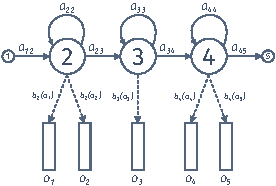
\includegraphics[width=0.7\textwidth]{./ch4-asr/img/hmm_structure.pdf}
  \caption{Příklad levo-pravého Markovova modelu trifónu}
  \label{fig:asr:acoustic:hmm}
\end{figure}

Pokud předpokládáme, že posloupnost slov $W$ je modelována zřetězeným skrytým Markovovým modelem $\lambda$, kde dílčí modely odpovídají fonetickým jednotkám, pak je možné určit pravděpodobnost generování posloupnosti $O$ modelem $\lambda$ jako

\begin{equation}
  P\left(O|\lambda\right) = \sum_{\forall S} P\left(O, S| \lambda\right)P\left(S|\lambda\right) = \sum_{\forall S} a_{s\left(0\right)s\left(1\right)} \prod_{t=1}^{T} b_{s\left(t\right)}\left(o_t\right)a_{s\left(t\right)s\left(t+1\right)},
  \label{eq:asr:acoustic:structure:output}
\end{equation}

\noindent kde posloupnost stavů $S = \left\{s\left(0\right), s\left(1\right),\dots, s\left(T+1\right)\right\}$ je chápána tak, že $s\left(0\right)$ je výstpní a $s\left(T+1\right)$ výstupní neemitující stav modelu $\Theta$ dané promluvy \cite{Psutka2006}. Přitom tento model lze značit trojicí

\begin{equation}
  \lambda = \left[\left\{a_{ij}\right\}_{k,s=1}^{I}; \left\{b_s(.)\right\}_{s=1}^{I};\left\{\pi_{s}\right\}_{s=1}^{I}\right],
  \label{eq:asr:acoustic:structure:marking}
\end{equation}

\noindent kde $a_{ij}$ je přechodová a $b_s(.)$ výstupní pravděpodobnost. Dále $\pi_s$ je rozložení pravděpodobnosti počátečního stavu a $I$ je počet stavů modelu.

Přímé vyčíslení pravděpodobnosti $P\left(O|\lambda\right)$ podle vztahu (\ref{eq:asr:acoustic:state:output}) je z hlediska počtu operací často nerealizovatelné, protože se jedná řádově o $2TN^{T}$ operací násobení. Z tohoto důvodu se proto využívá výpočetně efektivnější tzv. \textbf{algoritmus forward-backward (FB)} s přibližně $N^{2}T$ operací násobení.

Při výpočtu odpředu (forward) se určuje pravděpodobnost $\alpha_j\left(t\right)$ definovaná vztahem

\begin{equation}
  \alpha_{j}\left(t\right) = P\left(o_1o_2\dots o_t, s\left(t\right)=s_j|\lambda\right),
  \label{eq:asr:acoustic:structure:forward}
\end{equation}

\noindent pro výpočet odzadu (backward) se určuje pravděpodobnost $\beta_j\left(t\right)$ definována vztahem


\begin{equation}
  \beta_j\left(t\right) = P\left(o_{t+1}o_{t+2}\dots o_T|s\left(t\right)=s_j|\lambda\right).
  \label{eq:asr:acoustic:structure:backward}
\end{equation}

Podle \cite{Psutka2006} lze snadno dokázat, že výsledná pravděpodobnost $P\left(O|\lambda\right)$ může být vyčíslena vztahem

\begin{equation}
  P\left(O|\lambda\right) = \sum_{s=1}^{N} P\left(O, s\left(t\right) = s | \lambda\right) = \sum_{i = 1}^{N} \alpha_{i}\left(t\right)\beta_{i}\left(t\right)
  \label{eq:asr:acoustic:structure:forward-backward}
\end{equation}

\noindent pro $1 \leq t \leq T$.

\subsection{Trénování parametrů HMM s Gausovkými směsmi}
\label{chap:asr:acoustic:GMM}

Volba struktrury skrytého Markovova modelu je spíše expertní úlohou návrhu. Stanovéní hodnot parametrů modelu je uskutečněno trénováním (odhadem, etimací) na základě trénovacích akustických dat a jejich textových anotací (tzv. korpus). Pro trénování parametrů se využívá tzv. Baum-Welchův interativní algoritmus, což je speciální případ EM algoritmu. Více o něm v \cite{Holmes2001}. Pro odhad střední hodnoty $\mu_{sj}$, tj. složky $m$ gaussovské směsi ve stavu $j$ slouží vztah

\begin{equation}
  \hat{\mu}_{jm} = \frac{\sum_{t=1}^{T}\gamma_{jm}\left(t\right)o_t}{\sum_{t=1}^{T}\gamma_{jm}\left(t\right)},
  \label{eq:asr:acoustic:structure:mu}
\end{equation}

\noindent kde $N$ je počet stavů a $M$ počet složek. Také platí $1 \leq j \leq N$ a $1 \leq m \leq M$. Odhad kovarianční matice $C_{jm}$, tj. složky náležící m-té složce gaussovské směsi ve stavu $j$

\begin{equation}
  \hat{C}_{jm} = \frac{\sum_{t=1}^{T} \gamma_{jm}\left(t\right)\left(o_t - \hat{\mu}_{jm}\right)\left(o_t - \hat{\mu}_{jm}\right)^{T}}{\sum_{t=1}^{T}\gamma_j\left(t\right)},
  \label{eq:asr:acoustic:structure:covariant}
\end{equation}

\noindent kde $1 \leq j \leq N$ a $1 \leq m \leq M$. Odhad váhové složky hustotní směsi $c_{jm}$, tj. složky náležící složce $m$ gaussovské směsi ve stavu $j$ se provádí vztahem

\begin{equation}
  \hat{c}_{jm} = \frac{\sum_{t=1}^{T} \gamma_{jm}\left(t\right)}{\sum_{t=1}^{T}\gamma_j\left(t\right)},
  \label{eq:asr:acoustic:structure:weight}
\end{equation}

\noindent kde $1 \leq j \leq N$ a $1 \leq m \leq M$. Přitom $\gamma_{j}\left(t\right)$ představuje přavděpodobnost, že proces generování posloupnosti $O$ je v čase $t$ ve stavu $j$. Pro vyjádření této pravděpodobnosti $\gamma_{j}\left(t\right)$ platí rovnice (\ref{eq:asr:acoustic:structure:forward-backward}). Pro její definování pak platí vztah

\begin{equation}
 \gamma_{j}\left(t\right) = \frac{P\left(O, s\left(t\right)=j|\lambda\right)}{P\left(O|\lambda\right)} = \frac{\alpha_{j}\left(t\right)\beta_{j}\left(t\right)}{P\left(O|\lambda\right)} ,
  \label{eq:asr:acoustic:structure:gamma}
\end{equation}

\noindent kde $j = 1,\dots,N$ a $t = 1, \dots, T$. Pravděpodobnost, že proces generování posloupnosti $O$ je v čase $t$ ve stavu $j$ a generuje složku $m$ gaussovské hustotní směsi

\begin{equation}
  \gamma_{jm}\left(t\right) = \frac{P\left(O, s\left(t\right)=j, m\left(j,t\right)=m|\lambda\right)}{P\left(O|\lambda\right)} = \frac{\alpha_{j}\left(t\right)\beta_{j}\left(t\right)}{P\left(O|\lambda\right)} \frac{c_{jm}\mathcal{N}\left(o_t;\mu_{jm}; C_{jm}\right)}{\sum_{i=1}^{M} c_{ji} \mathcal{N}\left(o_t;\mu_{ji};C_{ji}\right) }.
   \label{eq:asr:acoustic:structure:gamma:one}
 \end{equation}

\noindent Rozdělení výstupní pravděpodobnosti $b_j\left(o_t\right)$ pro emitující stav $j$ pak má tvar

\begin{equation}
   b_{j}\left(o_t\right) = \sum_{m=1}^{M} \hat{c}_{jm} \mathcal{N}\left(o_t; \hat{\mu}_{jm}; \hat{C}_{jm}\right).
   \label{eq:asr:acoustic:gmm:output}
 \end{equation}

\noindent Akustické modely postavené na kombinaci skrytých Markovových modelů a gaussovských směsí pracují s 10 až 100 tisíc hustotních směsí. Při dimenzi příznakového vektoru (viz \ref{chap:asr:parametrization}) vektoru například $45$ je často nutné provést odhad až 10 miliónů parametrů.

\subsection{Využití neuronových sítí}
\label{chap:asr:acoustic:DNN}

Neuronové sítě se inspirují neuronem v mozku člověka. Ukázka stavby neuronové buňky je znázorněna na obr. \ref{fig:asr:acoustic:dnn:neuron:human}. Dendrity jsou kráktké výběžky, které slouží k příjímání vstupních informací od ostatních neuronů nebo nervů. V tělo neuronu (soma) dochází k reakci na vstupní signály a vytvoření přísušné odezvy. Ta se dále šíří pomocí výběžku nazvaného axon. Jeho délka může dosahovat až 100 cm. Axon je přes synapse spojen s jinými neurony nebo dalšími buňkami v těle.

\begin{figure}[hbpt]
  \centering
  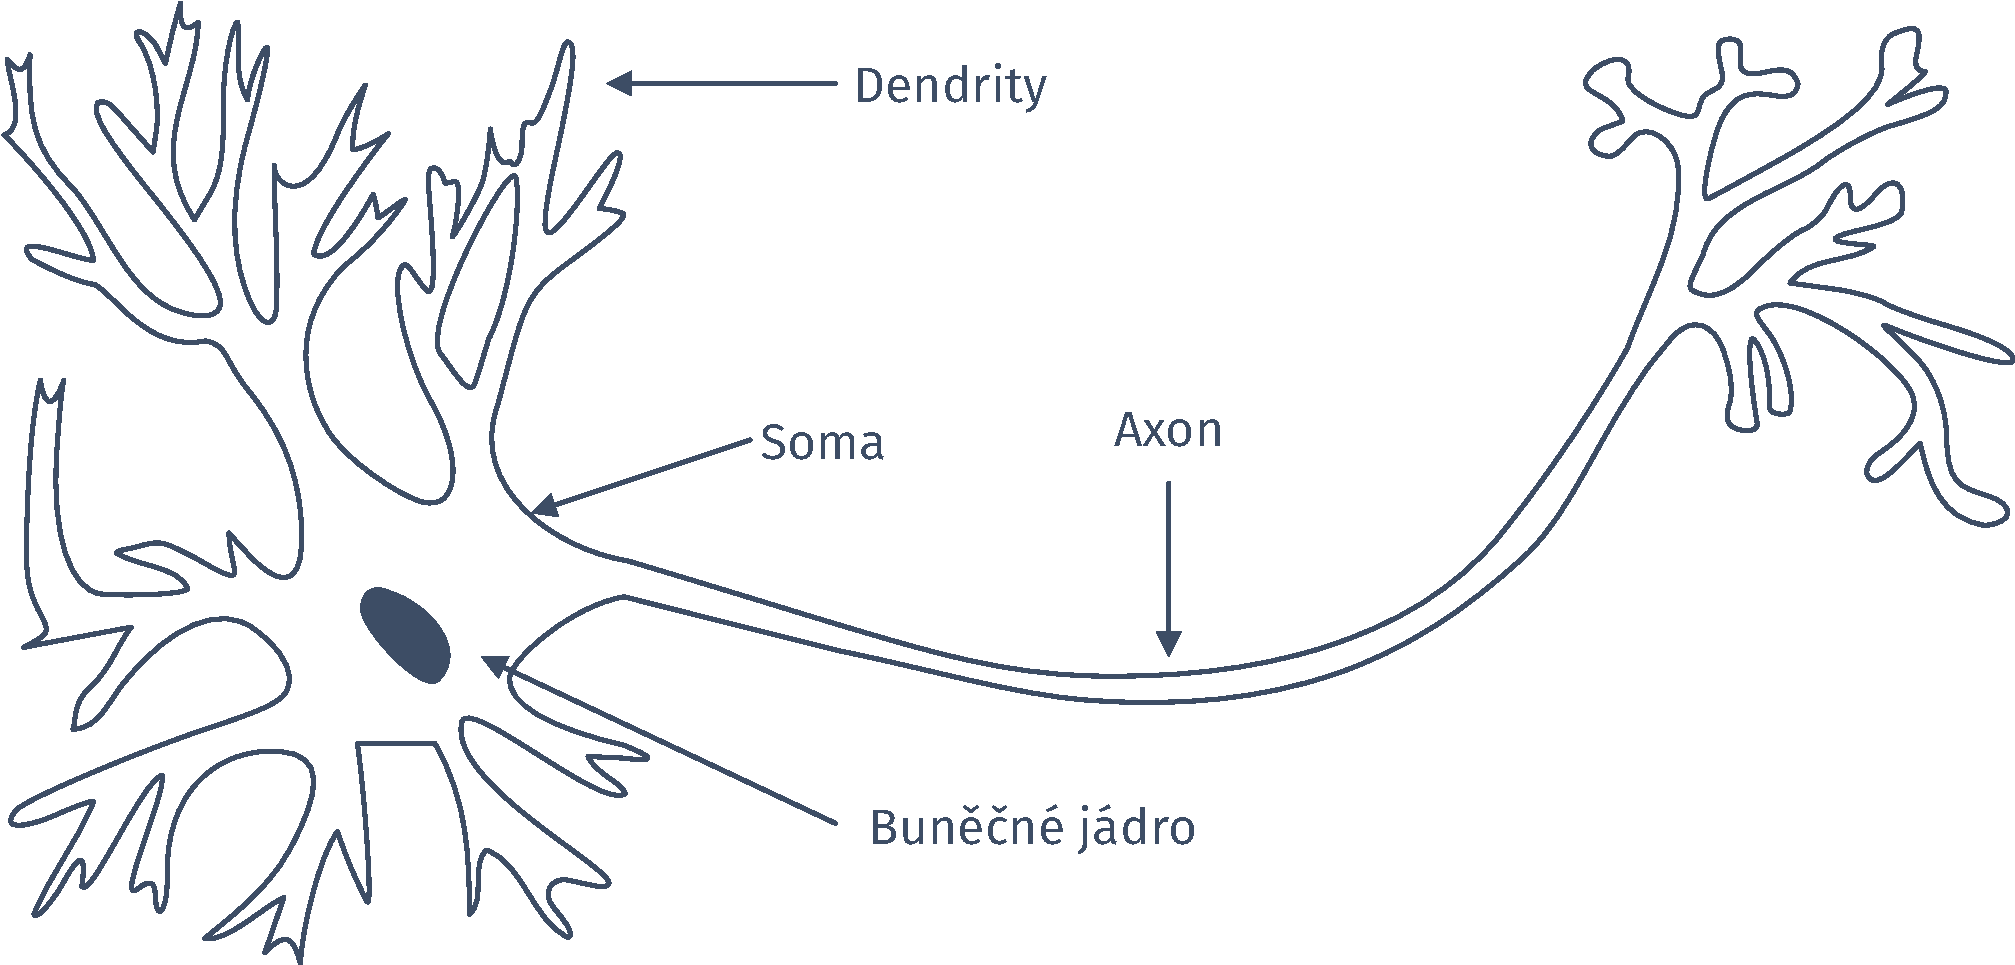
\includegraphics[width=0.7\textwidth]{./ch4-asr/img/neuron-human.pdf}
  \caption{Ukázka neuronové buňky}
  \label{fig:asr:acoustic:dnn:neuron:human}
\end{figure}

Umělý ekvivalent s názvem perceptron byl vytvořen Frankem Roseblattem v první polovině 60. let 20. století \cite{Rosenblatt1962}. Schématicky je zobrazen na obr. \ref{fig:asr:acoustic:dnn:neuron:artificial}. Matematicky lze princip neuronu popsat vztahem

\begin{equation}
  \hat{y}\left(x\right) = \sigma\left(z\right) = \sigma \left(w^{T}x + b\right) = \sigma \left( \sum_{j=1}^{n} w_{j}x_{j} + b\right),
   \label{eq:asr:acoustic:dnn:neuron:output}
 \end{equation}

\noindent kde $x$ představuje vstupní vektor, $w$ váhový vektor a $b$ práh. Výsledek linární kombinace je vstupem aktivační funkce $\sigma\left(.\right)$, jejíž výstup je zároveň výstupem neuronu. Neuronová síť\footnote{Popisovaná neuronová síť je typu feedforward (FF). Dalšími typy sítí jsou konvoluční a rekurentní neuronové sítě. Oproti FF síti se liší hlavně svou strukturou. Princip propojení neuronových buněk je však stejný.} (NN, viz obr. \ref{fig:asr:acoustic:dnn:training}) je složena z jedné či více vrtev neuronů. V případě více vrstvé NN jsou vždy propojeny neurony mezi vrstavami $l$ a $l+1$.

\begin{figure}[hbpt]
  \centering
  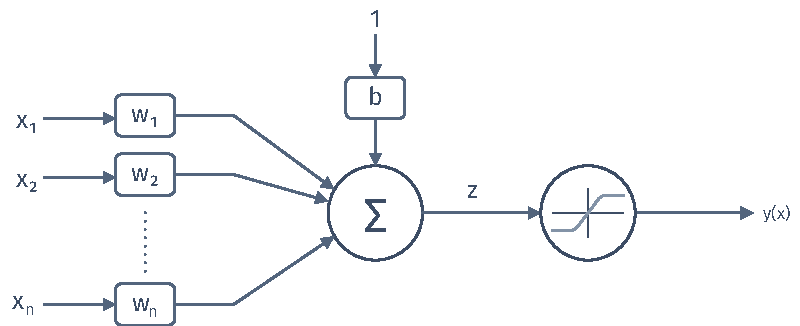
\includegraphics[width=0.7\textwidth]{./ch4-asr/img/neuron.pdf}
  \caption{Schéma perceptronu}
  \label{fig:asr:acoustic:dnn:neuron:artificial}
\end{figure}

Zmíněná aktivační funkce hraje velmi významnou roli, protože umožňuje řešení i nelineárních problémů. Pokud by NN nevyužívala aktivační funkce, jednalo by se defakto stále o lineární kombinaci vektorů a tím pádem by bylo možné řešit jen linární problémy. Mezi nejčastěji používané patří \textit{sigmoid} ($\sigma\left(z\right) = \left(1 - e^{-z}\right)^{-1}$), \textit{tanh} a \textit{relu} ($\sigma\left(z\right) = \max\left(0, z\right)$). Průběhy těchto aktivačních funkcí jsou vidět na obr. \ref{fig:asr:acoustic:dnn:activation}.

 \begin{figure}[htpb]
  \centering
  \begin{subfigure}[b]{0.29\textwidth}
    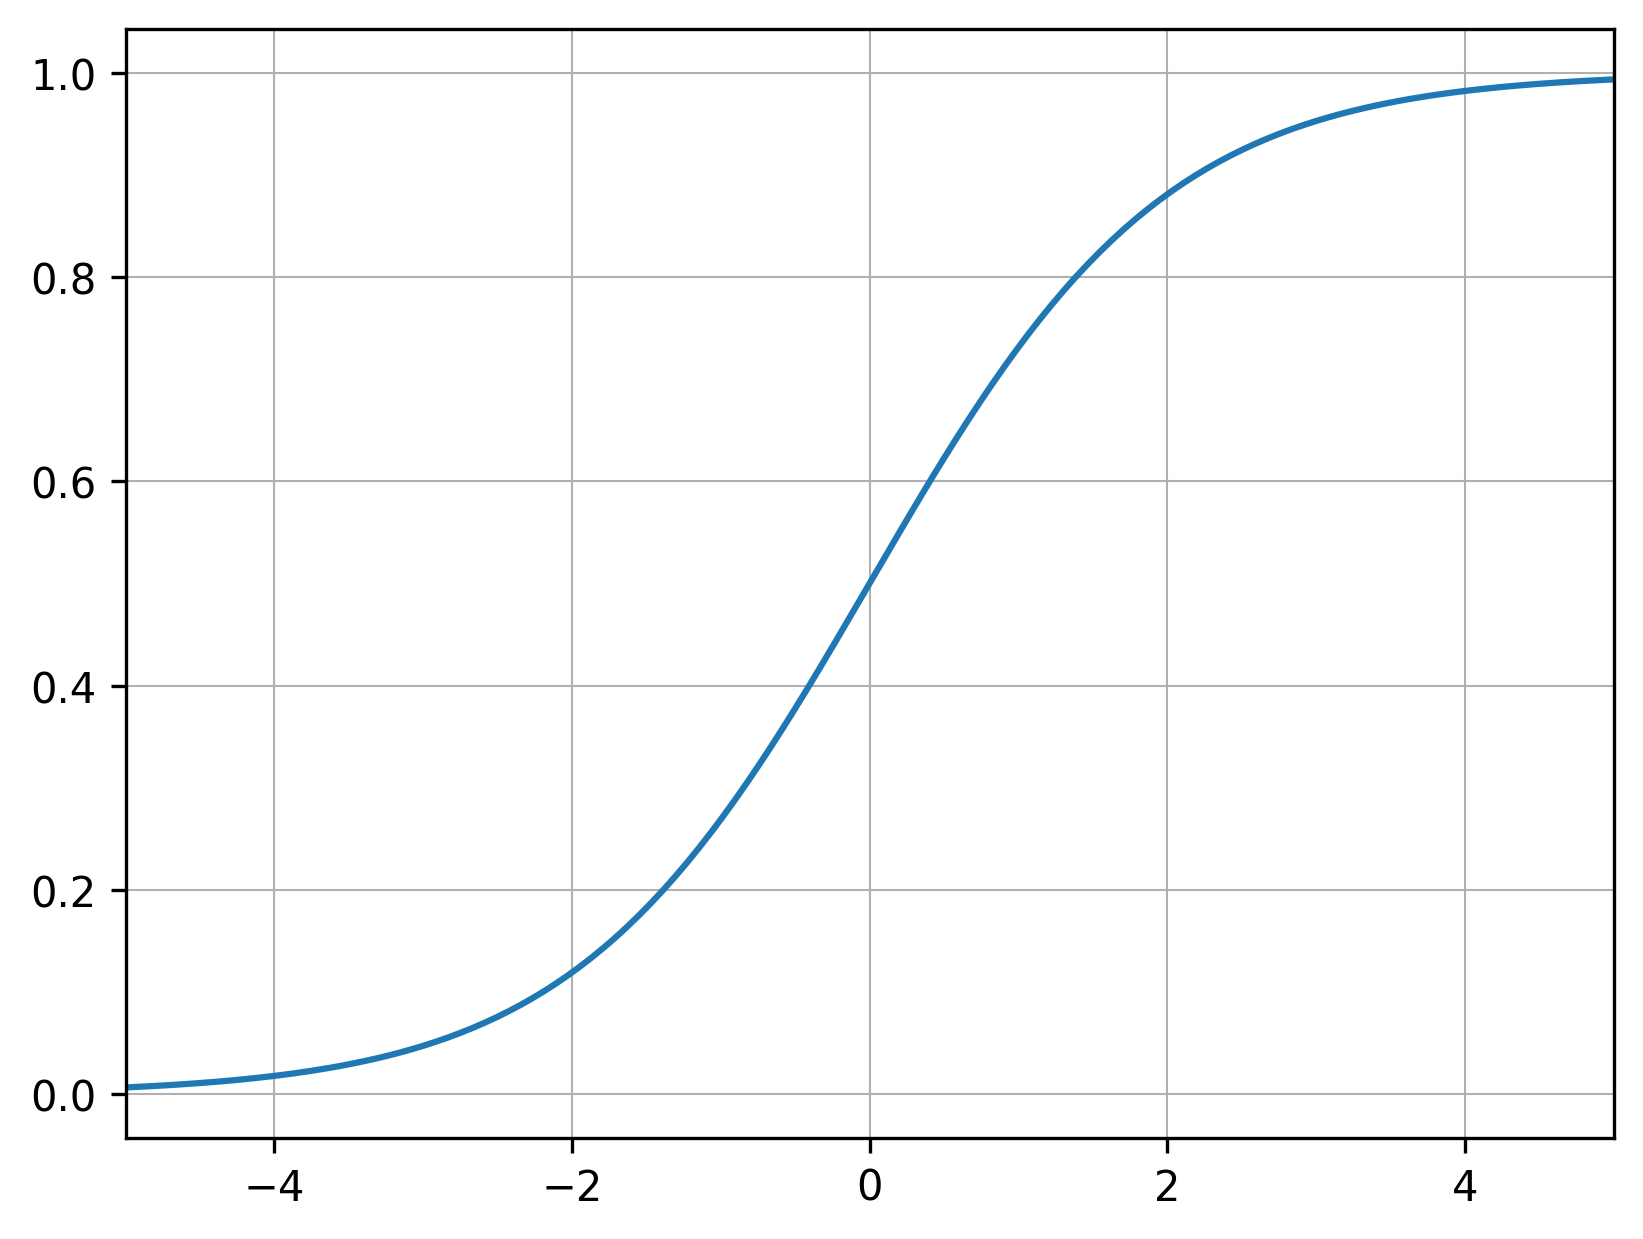
\includegraphics[width=\textwidth]{./ch4-asr/img/sigmoid.png}
    \caption{sigmoid}
    \label{fig:asr:acoustic:dnn:activation:sigmoid}
  \end{subfigure}
  %
  \begin{subfigure}[b]{0.3\textwidth}
    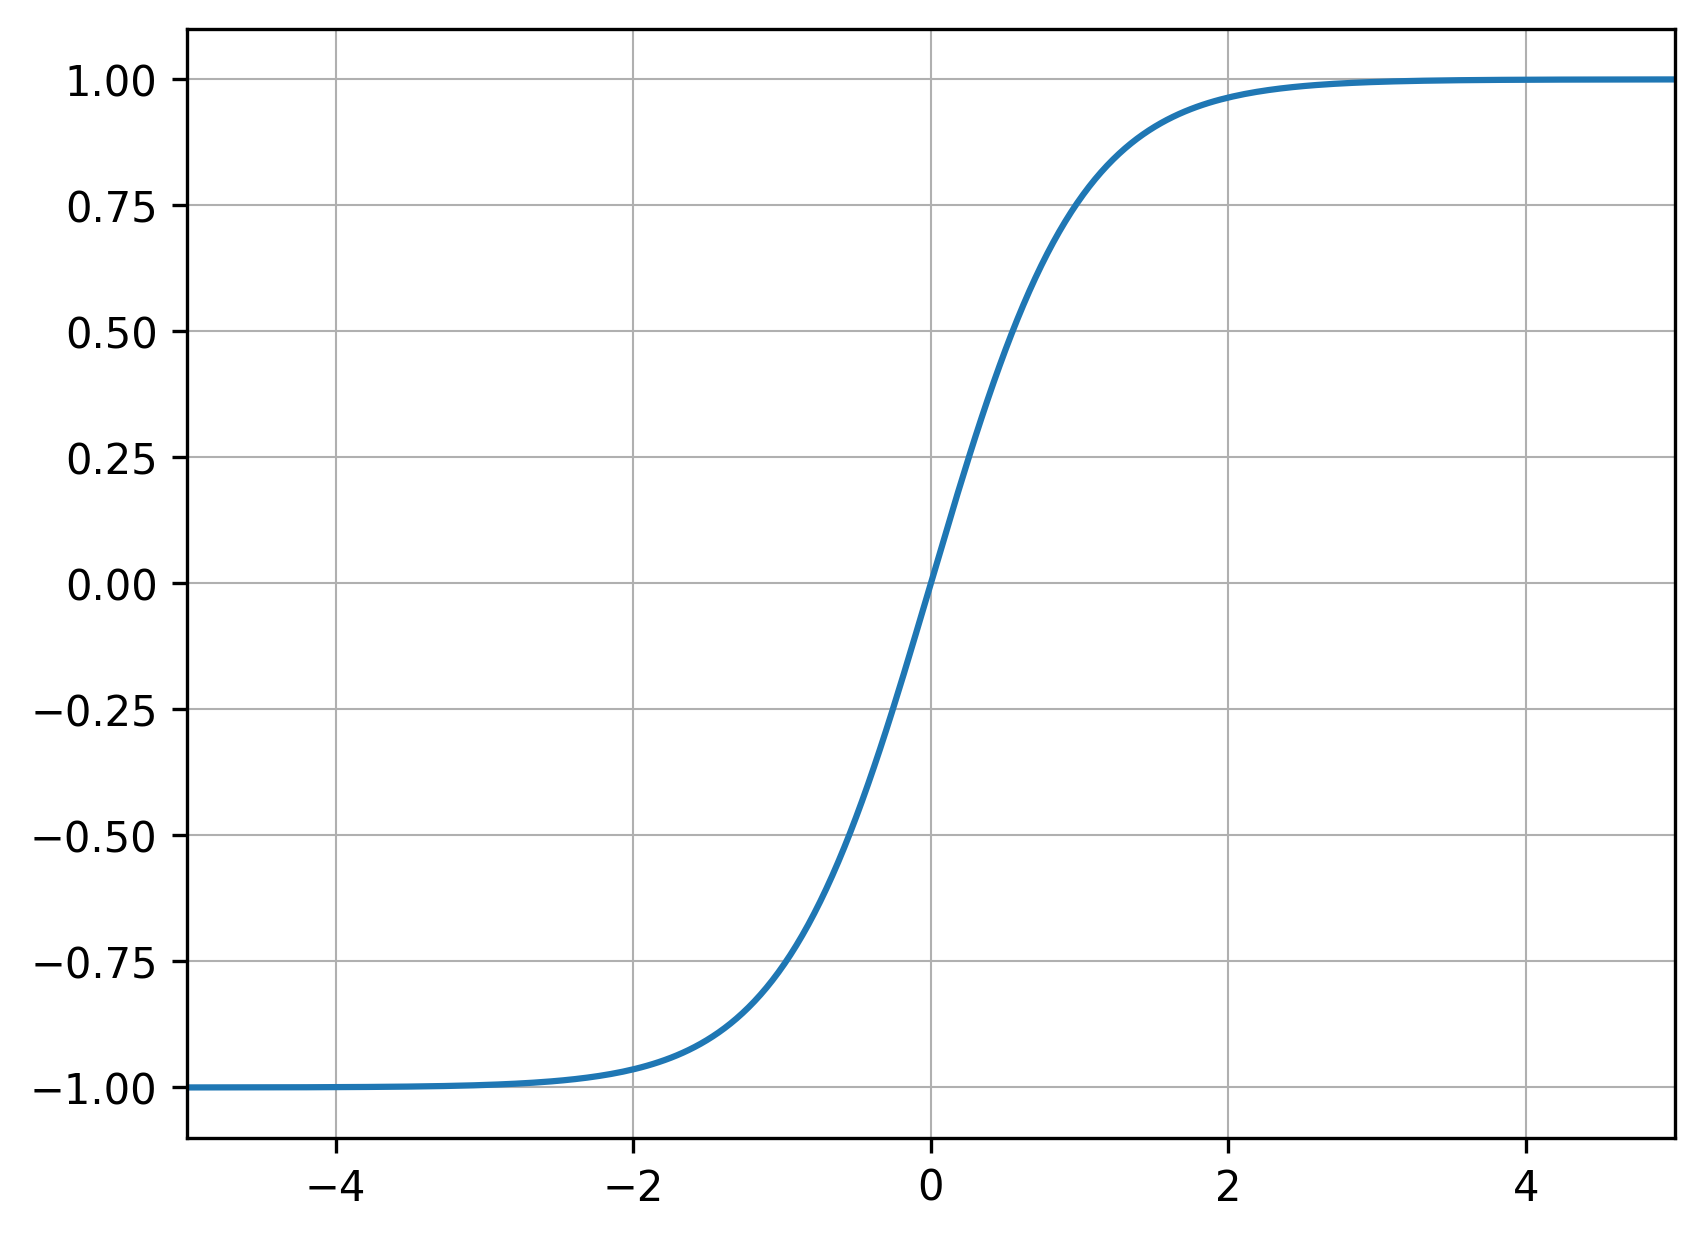
\includegraphics[width=\textwidth]{./ch4-asr/img/tanh.png}
    \caption{tanh}
    \label{fig:asr:acoustic:dnn:activation:tanh}
  \end{subfigure}
  %
  \begin{subfigure}[b]{0.28\textwidth}
    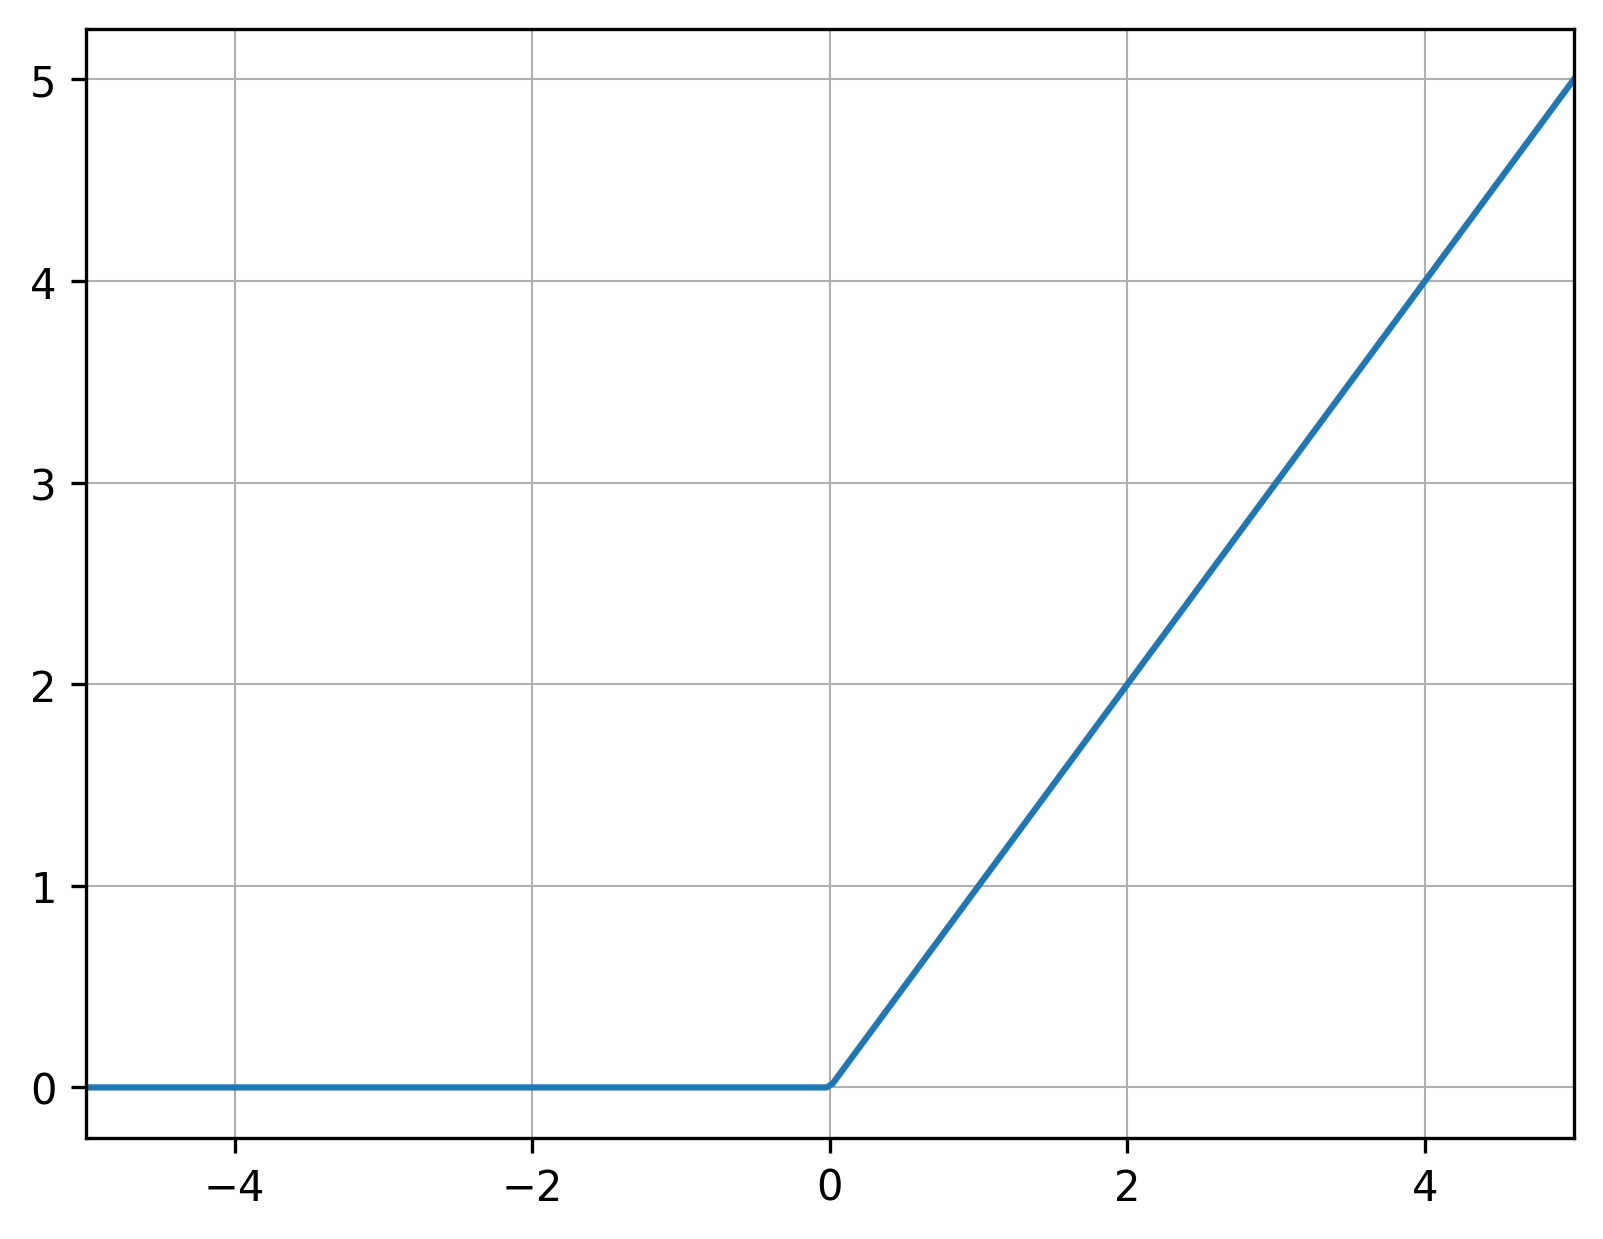
\includegraphics[width=\textwidth]{./ch4-asr/img/relu.png}
    \caption{relu}
    \label{fig:asr:acoustic:dnn:activation:relu}
  \end{subfigure}
  \caption{Příklady používaných aktivačních funkcí}
  \label{fig:asr:acoustic:dnn:activation}
\end{figure}

Pro výpočet výstupu neuronové sítě, tzv. \textbf{forward propagation}, je použit iterativní postup matematicky zapsán jako

\begin{align}
  \begin{split}
    Z^{[l]} = W^{[l]}a^{[l-1]} + b^{[l]}, \\
    a^{[l]} = \sigma^{[l]}\left(Z^{[l]}\right),
  \end{split}
  \label{eq:asr:acoustic:dnn:fw}
\end{align}

\noindent kde $a^{[l]}$ představuje výstup $l$-té vrstvy ($a^{[0]} = x$), $W^{[l]}$ představuje váhovou matici $l$-té vrstvy, $b^{[l]}$ vektor prahů $l$-té vrstvy a $\sigma^{[l]}(.)$ aktivační funkci $l$-té vrstvy. Pro $l$ platí $l = 1, \dots, N$, kde $N$ je počet vrstev neuronové sítě. Výsledkem iterativního výpočtu (\ref{eq:asr:acoustic:dnn:fw}) je výstup sítě $y = a^{[N]}$.

Trénováním neuronové sítě je myšleno určení hodnot váhových matic $W^{[l]}$ a prahů $b^{[l]}$. Tento proces se iterativně sestává ze 3 kroků (viz obr. \ref{fig:asr:acoustic:dnn:training})

\begin{enumerate}
  \item výpočet výstupu sítě (\ref{eq:asr:acoustic:dnn:fw}),
  \item vypočtení chyby predikce $J\left(y, \hat{y}\right)$,
  \item aktualizace vah pomocí algoritmu backpropagation.
\end{enumerate}

\noindent Výpočet výstupu NN je realizován pomocí (\ref{eq:asr:acoustic:dnn:fw}), dále tedy nezbytné vypočítat chybu predikce $J\left(y, \hat{y}\right)$, Ta je difinována vztahem

\begin{equation}
  J\left(y, \hat{y}\right) = \frac{1}{m} \sum_{i=1}^{m}\mathcal{L}\left(y, \hat{y}\right),
  \label{eq:asr:acoustic:dnn:cost}
\end{equation}

\noindent kde $m$ je počet prvků trénovací množiny a $\mathcal{L}\left(y, \hat{y}\right)$ je funkce výpočtu chyby predikce $m$-tého prvku trénovací množiny. Konkrétní funkce závisí na typu řešené úlohy, ale často se používá cross-entropie definované vztahem

\begin{equation}
  \mathcal{L}\left(y, \hat{y}\right) = - \sum_{i=1}^{m} y_i \log \hat{y}_i,
  \label{eq:asr:acoustic:dnn:cost}
\end{equation}

\noindent kde $m$ je dimenze výstupního vektoru.

Samotná aktualizace parametrů sítě je realizování \textbf{backpropagation} algoritmem. Cílem tohoto algoritmu je vypočtení parciálních derivací $\partial J / \partial W^{[l]}$ a $\partial J/\partial b^{[l]}$. Tyto parciální derivace je potřeba vypočíst pro všechny vrstvy sítě. Chyba ve vrstvě $l$ je závislá na chybě v předchozí vrstvě $l-1$. Tato skutečnost znamená, že je možné použít tzv. chain pravidlo. Parciální derivace pak mají následující podobu

\begin{align}
  \begin{split}
    \frac{\partial J}{\partial W^{[l]}} & = \frac{\partial J}{\partial a^{[l]}} \frac{\partial a^{[l]}}{\partial z^{[l]}} \frac{\partial z^{[l]}}{\partial W^{[l]}}, \\
    \frac{\partial J}{\partial b^{[l]}} & = \frac{\partial J}{\partial a^{[l]}} \frac{\partial a^{[l]}}{\partial z^{[l]}} \frac{\partial z^{[l]}}{\partial b^{[l]}}
  \end{split}
  \label{eq:asr:acoustic:dnn:partial}
\end{align}

\noindent Vzorce pro výpočet aktualizací parametrů sítě jsou pak následující

\begin{align}
  \begin{split}
    \delta^{[L]} & = \nabla_{a} J \odot \sigma'\left(z^{[L]}\right), \\
    \delta^{[l]} & = \left(\left(w^{[l+1]}\right)^T \delta^{[l+1]}\right) \odot \sigma'\left(z^{[l]}\right), \\
    \frac{\partial J}{\partial W^{[l]}} & = a^{[l-1]}\delta^{[l]}, \\
    \frac{\partial J}{\partial b^{[l]}} & = \delta^{[l]},
  \end{split}
  \label{eq:asr:acoustic:dnn:bp}
\end{align}

\noindent kde $\nabla_a J = \partial J / \partial a^{[L]}$ a $\odot$ představuje Hadamardův součin. Samotná aktualizace parametrů je realizována vztahy

\begin{align}
  \begin{split}
    W^{[l]} & = W^{[l]} - \alpha \frac{\partial J}{\partial W^{[l]}}, \\
    b^{[l]} & = b^{[l]} - \alpha \frac{\partial J}{\partial b^{[l]}},
  \end{split}
  \label{eq:asr:acoustic:dnn:update}
\end{align}

\noindent kde $\alpha$ reprezentuje koeficient učení.

\begin{figure}[hbpt]
  \centering
  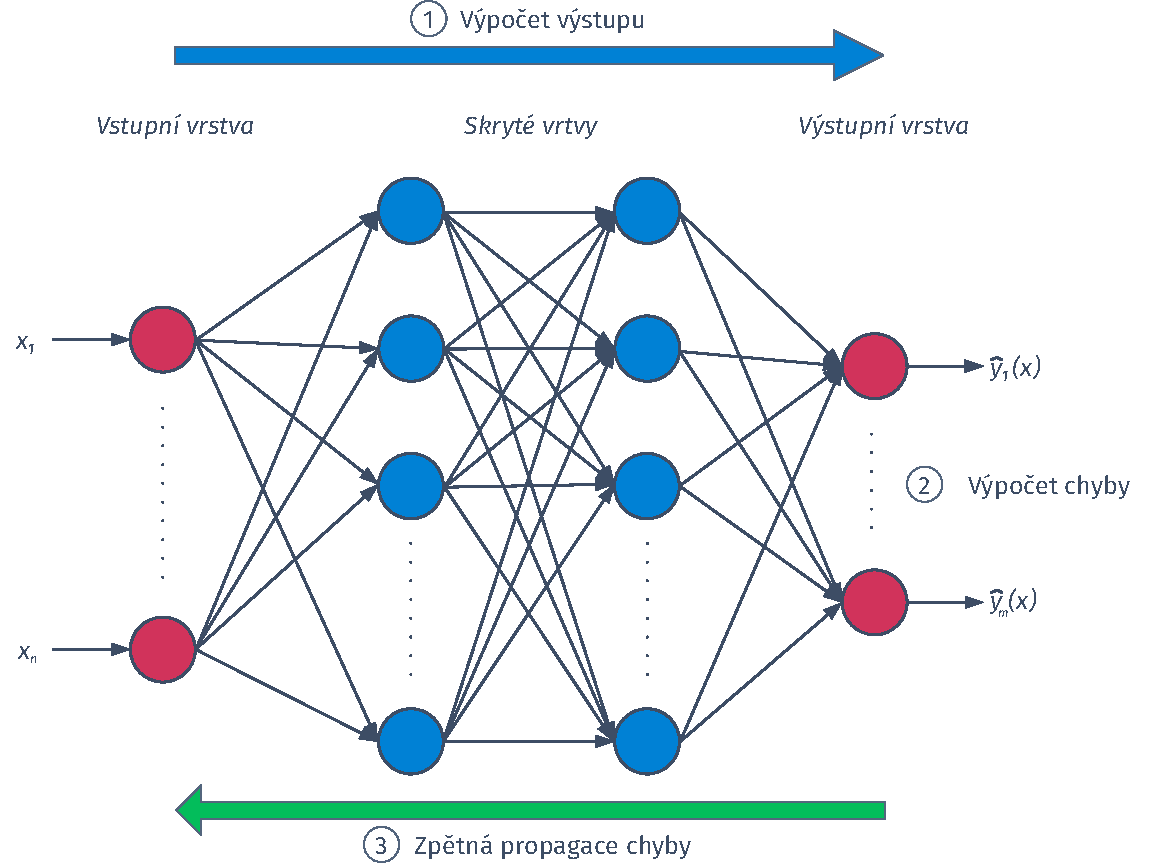
\includegraphics[width=0.9\textwidth]{./ch4-asr/img/dnn-training.pdf}
  \caption{Schéma a princip učení neuronové sítě}
  \label{fig:asr:acoustic:dnn:training}
\end{figure}

\subsubsection{Spojení skrytých Markovových modelů a neuronových sítí}

Rozvoj výpočetní techniky, zejména GPU\footnote{Graphics Processing Unit} s možností provádět obecné maticové operace, zapříčinil masivní využití tzv. hlubokých neuronových sítí (DNN). Ty se vyznačují vyšším počtem skrytých vrstev, což umožňuje řešit sofistikovanější problémy. Jedním takovým je rozpoznávání souvislé řeči. Bohužel DNN end-to-end\footnote{Systém, který kompletně řeší rovnici (\ref{eq:asr:decoding:generic}) pomocí jediné DNN sítě. Tyto systémy jsou většinou postaveny na rekurentních neuronových sítích (RNN).} systém je zatím velmi komplikované vytvořit a provozovat zejména, proto že k uspěšnému natrénování je potřeba řádově více dat, než u GMM \cite{Amodei2016}. Z tohoto důvodu jsou v současné době nejčastější systémy postavené na kombinaci HMM a DNN (HMM-DNN). Rozdíl oproti end-to-end systému je v tom, že cílem DNN není odhad $\hat{W}$, ale ,stejně jako v případě HMM-GMM, určit $b_j\left(o_t\right)$.

V případě HMM-GMM je odhad $b_j\left(o_t\right)$ realizován gaussovskými hustotními směsmi podle vzorce (\ref{eq:asr:acoustic:gmm:output}). Těchto směsí je tolik, kolik je unikátních stavů HMM. U DNN však žádné směsi k dispozici nejsou. Pokud je všask výstupní vrstva typu \textbf{softmax}, kde výstup $j$-tého neuronu je definován vztahem

\begin{equation}
  y_{j} = a_{j}^{[L]} = \frac{e^{z_j}}{\sum_{i=1}^{m}e^{z_i}},
  \label{eq:asr:acoustic:dnn:asr:softmax}
\end{equation}

\noindent kde $m$ je počet neuronů v poslední vrstvě. Zároveň platí

\begin{equation}
  \sum_{j=1}^{m} y_{j} = 1.
  \label{eq:asr:acoustic:dnn:asr:softmax:criterium}
\end{equation}

\noindent Hodnoty výstupního vektoru $y$ mají pseudo-pravděpodobnostní charakter. Pokud tedy bude $m$ rovno počtu stavů $HMM$, pak výstupní pravděpodnost $b_{j} \left(o_t\right)$ pro emitující stav $j$ má, podle (\ref{eq:asr:acoustic:dnn:asr:softmax}), tvar

\begin{equation}
  b_{j} \left(o_t\right) = y_{j} = \frac{e^{z_j}}{\sum_{i=1}^{m}e^{z_i}}.
  \label{eq:asr:acoustic:dnn:asr:softmax:criterium}
\end{equation}

\noindent Principiální rozdíl ve funkci HMM-GMM a HMM-DNN je znázorněn na obr. \ref{fig:asr:acoustic:dnn:asr:diff}.

\begin{figure}[htpb]
  \centering
  \begin{subfigure}[b]{0.4\textwidth}
    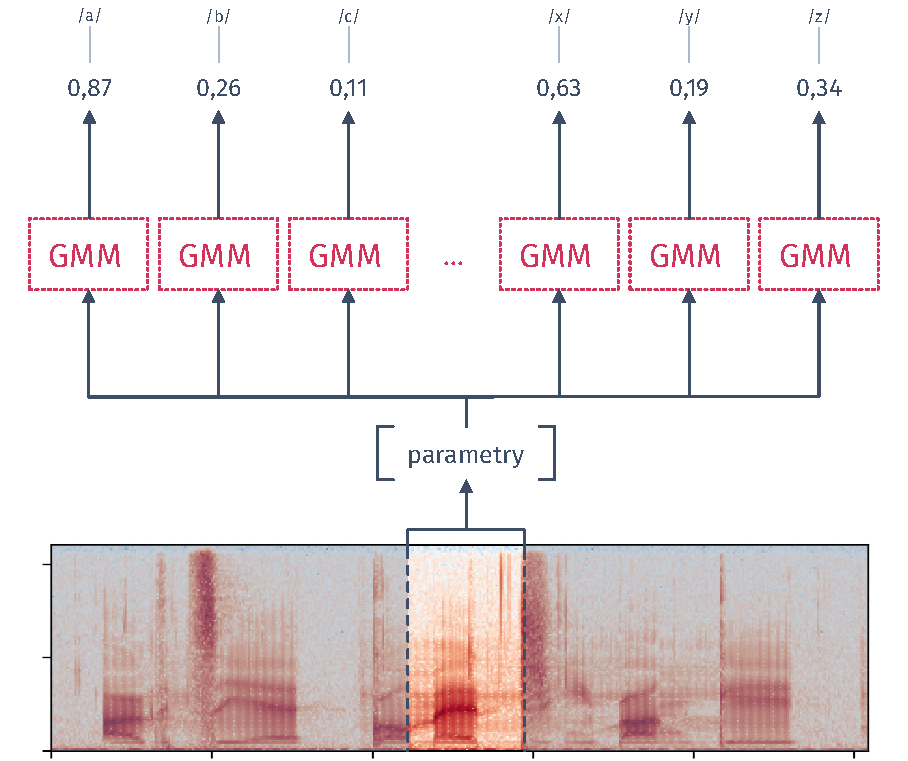
\includegraphics[width=\textwidth]{./ch4-asr/img/hmm-gmm.pdf}
    \caption{GMM}
    \label{fig:asr:acoustic:dnn:asr:diff:dnn}
  \end{subfigure}
  %
  \begin{subfigure}[b]{0.4\textwidth}
    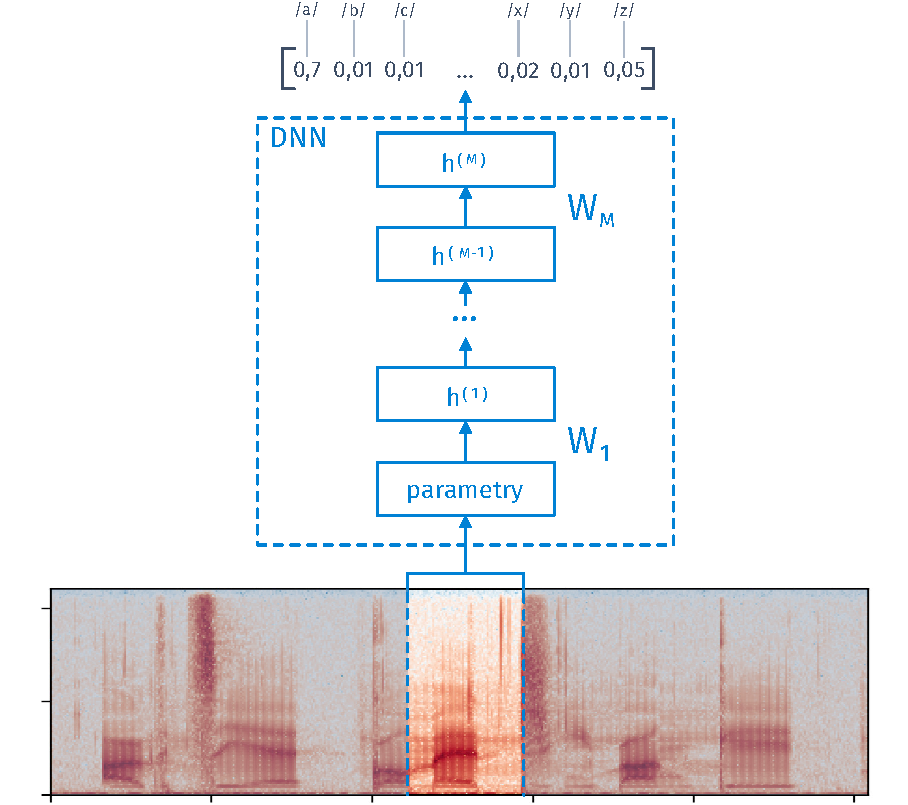
\includegraphics[width=\textwidth]{./ch4-asr/img/hmm-dnn.pdf}
    \caption{DNN}
    \label{fig:asr:acoustic:dnn:asr:diff:dnn}
  \end{subfigure}
  \caption{Principální rozdíl ve funkci GMM a DNN systému}
  \label{fig:asr:acoustic:dnn:asr:diff}
\end{figure}

K natrénování DNN se používá zmíněného backpropagation algoritmu. V poslední době se však prosadilo trénování využívající předtrénování DNN pomocí tzv. restricted Bolzmann machines (RBM) \cite{Hinton2012}. Předtrénování řeší problém kdy se informace zpětně propagovaná pomocí backpropagation algoritmu úplně neovlivní počáteční vrstvy, protože gradient je příliš malý. Předtrénování pomocí RBM pomáhá lépe určit parametry sítě. Princpálně je tento proces znázorněn na obr. \ref{fig:asr:acoustic:dnn:pretraining}.

Nejprve je natrénován GRBM (Gaussian-Bernoulli RBM) model na mikrosegmentu řeči složeného z několika okének parametrů odpovídající délce promluvy například $10\ ms$. Stav skrytých jednotek je použit k natrénování RBM. Tento proces se opakuje dokud není natrénován požadovaný počet vrstev výsledné sítě. Následně jsou jednotlivé RBM spojeny do deep belief sítě (DBN). Následně je přidána výstupní softmax vrstva dimenze rovné počtu HMM stavů (DBN-DNN). Tato DBN-DNN síť je pak diskriminativně trénována na základě zarovnání získaného pomocí HMM-GMM. Více o tomto principu trénování v \cite{Hinton2012} a \cite{Vesely2013}. Vstupem neuronové sítě je často mikrosegment $t$ a jeho okolní mikrosegmenty. Velmi často se používá okolí $t-2$ a $t+2$.

\begin{figure}[hbpt]
  \centering
  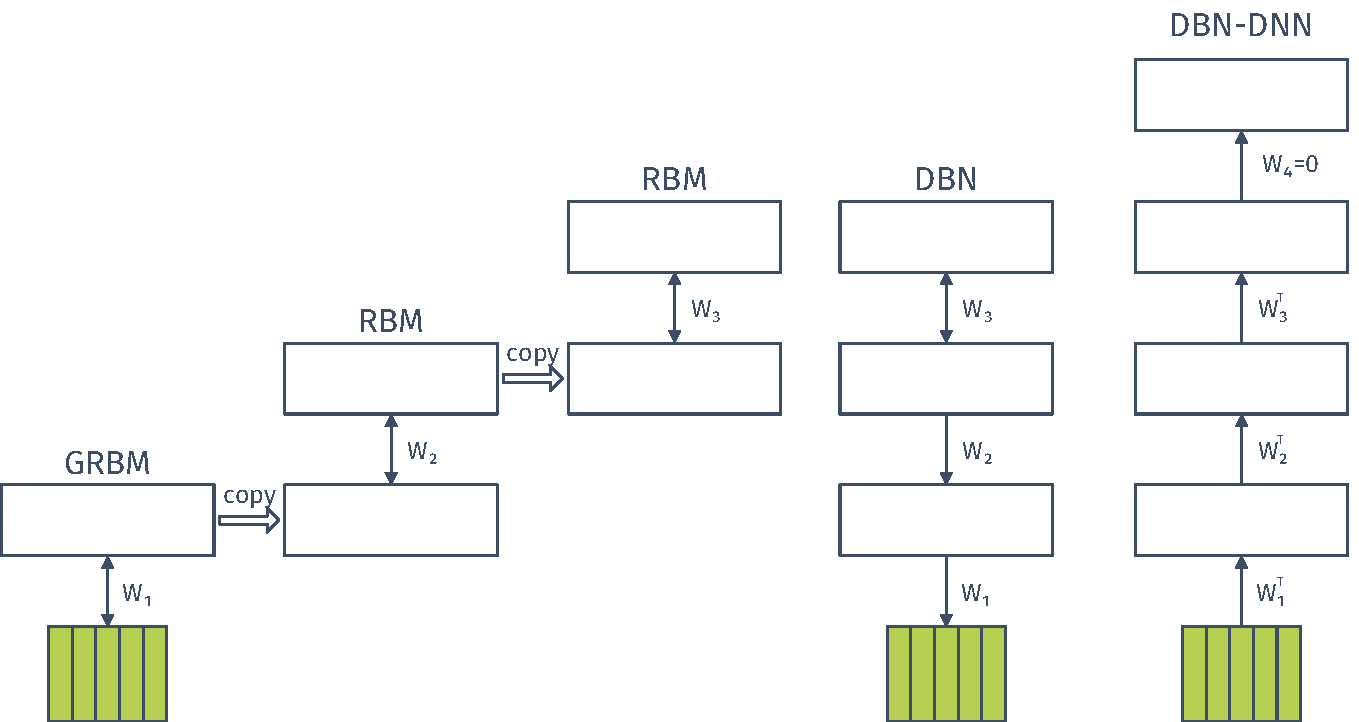
\includegraphics[width=0.9\textwidth]{./ch4-asr/img/pretraining.pdf}
  \caption{Princip předtrénování pomocí RBM s třemi vrstvami \cite{Hinton2012}.}
  \label{fig:asr:acoustic:dnn:pretraining}
\end{figure}

\subsubsection{Time-delay neural networks}

Nevýhodou DNN sítí je, že berou v potaz pouze statické parametry v rámci zpracovávaných mikrosegmentů, protože sumace v perceptronu odpovídá sumě vážených statických vstupů. Po zpracování segmentu $t$ není získaná informace nijak reflektována při zpracování segmentu $t+1$. Tento nedostatek by řešilo použití rekurentních neuronových sítí (RNN). Bohužel tyto sítě mají mnohem komplikovanější buňku neuronu než FF sítě s perceptronem \cite{Amodei2016}. Proto je potřeba řádově více dat k natrénování. Složitost buňky také zvyšuje komputační náročnost výpočtu.

Základním rozdílem sítí typu time-delay neural network (TDNN) (představená v \cite{Waibel1989}) je přidání časové filtrace do sumační části neuronu, tím je docíleno zahrnutí dynamické složky do výpočtu sítě \cite{Craig2000}. Filtrace je implementována jako filtr s konečnou impulzní odezvou (FIR), tedy

\begin{equation}
  z_{j}^{[l]}\left(t\right) = \sum_{n=0}^{N} w_{j}^{[-n]}f\left(n\right)a^{[l-1]}\left(t - n\right) + b_{j},
  \label{eq:asr:acoustic:dnn:tdnn:fir}
\end{equation}

\noindent kde $t$ je dikrétní časový index, $N$ je délka FIR filteru, $f\left(n\right)$ odezva filtru, $w_{j}^{[-n]}$ příslušná váha, $a^{[l-1]}$ je výstup vrstvy $l-1$ a $z_{j}^{[l]}\left(t\right)$ je výstup sumační části neuronu $j$ ve vrstvě $l$. Vztah (\ref{eq:asr:acoustic:dnn:tdnn:fir}) tedy představuje konvoluci. Na obr. \ref{fig:asr:acoustic:dnn:tdnn:neuron} je principiálně znázorněn neuron pracující s $N$ FIR filtry. Z obr. \ref{fig:asr:acoustic:dnn:tdnn:neuron} je také zřejmé, že TDNN síť má několik souborů vah $W^{x}$, které umožňují lépe pracovat s dynamickou složkou signálu \cite{Peddinti2015}.

\begin{figure}[htpb]
  \centering
  \begin{subfigure}[b]{0.45\textwidth}
    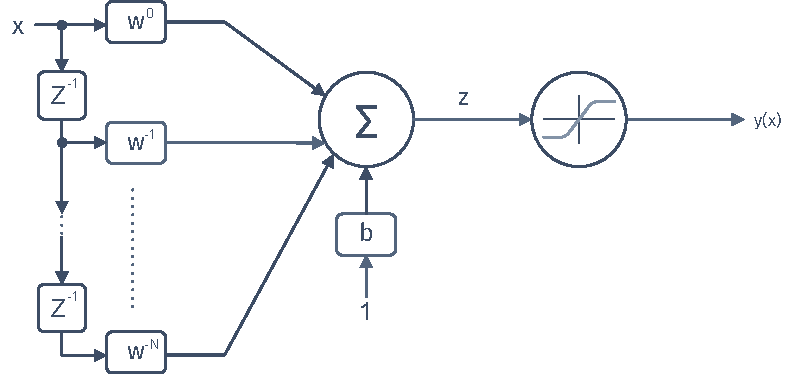
\includegraphics[width=\textwidth]{./ch4-asr/img/neuron-tdnn.pdf}
    \caption{neuron}
    \label{fig:asr:acoustic:dnn:tdnn:neuron}
  \end{subfigure}
  %
  \begin{subfigure}[b]{0.35\textwidth}
    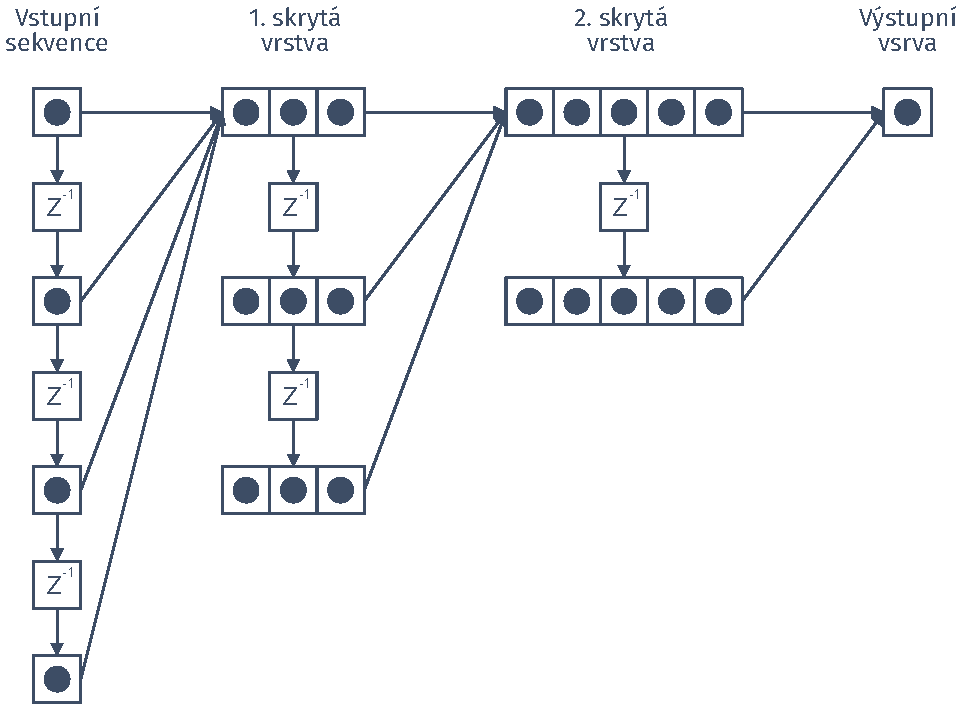
\includegraphics[width=\textwidth]{./ch4-asr/img/tdnn.pdf}
    \caption{síť}
    \label{fig:asr:acoustic:dnn:tdnn:net}
  \end{subfigure}
  \caption{Neuron TDNN sítě a jednoduché blokové schéma TDNN sítě \cite{Craig2000}}
  \label{fig:asr:acoustic:dnn:tdnn}
\end{figure}

Stejně jako v případě DNN sítě je vstupem parametrizovaný mikrosegment $t$ a jeho okolí. Z obr. \ref{fig:asr:acoustic:dnn:tdnn:net} je patrné, že hlubší vsrtvy postupně zpracovávájí větší a větší okolí mikrosegmentu $t$. Dimenze výstupní vrstvy odpovída počtu HMM stavů. Přestože je TDNN síť typu FF, tak dokáže pracovat i s dynamickými parametry řeči, protože využívá princip konvoluce.

% !TEX root = ../thesis.tex
\section{Jazykové modelování}
\label{chap:asr:language}

Jazykový model (obr. \ref{fig:asr:decoding}) je po parametrizaci a akustickém modelu další důležitou částí systému rozpoznávání řeči. Jeho úkolem je poskytnout dekodéru co nejrychleji nejpřesnější odhad apriorní pravděpodobnosti $P\left(W\right)$ pro libovolnou posloupnost slov $W$. Tuto pravděpodonost je možné vyjádřit vztahem

\begin{equation}
  P\left(W\right) = \prod_{k=1}^{K} P\left(w_k | w_{k-1}\dots w_{1}\right),
  \label{eq:asr:language:W_full}
\end{equation}

\noindent kde $K$ je počet slov posloupnosti $W$. Pokud by byl proveden rozklad (\ref{eq:asr:language:W_full}) vyšlo by najevo, že pravděpodobnost výskytu slova $P\left(w_i\right),\ i \leq K$ je podmíněna pouze svou historií, tj. posloupností slov $w_1\ \dots\ w_{i-2}w_{i-1}$.

Systémy rozpoznávání řeči pracují obvykle s rozsáhlými slovníky, čítající stovky tisíc až jednotky milionů slov, není možné předpokládat, že by bylo možné pravděpodobnosti v (\ref{eq:asr:language:W_full}) dostatečně robustně odhadnout pro libovolnou délku posloupnosti $K$.

Obvykle se proto provádí aproximace vztahu (\ref{eq:asr:language:W_full}), při níchž docházi k redukci počtu odhadovaných parametrů. Nejčastějším způsobem je stanovení ekvivalentních tříd slov na základě jejich slovní historie, tj. všechny historie $w_1\ \dots\ w_{i-2}w_{i-1}$, které se shodují v posledních $n-1$ slovech, jsou zařazeny do stejné třídy. Uvedené modely se nazývají \textbf{n-gramové modely}. Přitom \textit{n}-gramem se rozumí posloupnost $n$ za sebou jdoucích slov v pozorování jejich náhodného výběru, např. trénovacího korpusu obsahujícího textová data. Modely s $n=0$ se nazývají \textbf{zerogramy}, $n=1$ pak \textbf{unigramy}. Nejpoužívanější jsou pak \textbf{bigramy} ($n=2$) a \textbf{trigramy} ($n=3$). Pravděpodobnost $P\left(W\right)$ u $n$-gramového modelu se vypočte vztahem

\begin{equation}
  P\left(W\right) = \prod_{k=1}^{K} P\left(w_k | w_{k-1}\dots w_{k-n+1}\right).
  \label{eq:asr:language:W}
\end{equation}

\noindent V ideálním případě by optimální model měl mít $n > 3$, ale v praxi se tyto modely moc nepoužívají, protože s rostoucím řádem modelu enormně roste potřebná velikost trénovacích dat. Například pro slovník s $N$ položkami existuje stále $N^{n}$ $n$-gramových statistik, které je potřeba odhadnout. Jak bylo zmíněno odhad těchto statistik se provádí na základě relativních četností v trénovacích datech. Například u bigramů ($n=2$) a slovníku o velikosti $N=10^{5}$ je zapotřebí odhadnout $10^{10}$ různých bigramů a k tomu je zapotřebí relativně velké trénovací množiny. Je zřejmé, že většina z těchto $10^{10}$ bigramů se vůbec neobjeví v datech. Těmto \uv{neviděným} bigramům tedy odpovídá nulová pravděpodobnost, což vyústí v nulovou pravděpodobnost $P\left(W\right)$ (\ref{eq:asr:language:W}). K řešení tohoto problému se používá technik \uv{vyhlazování}. Jejich cílem je odhad pravděpodobností těchto neviděných jevů s využitím tzv. ústupových, interpolačních a diskontních schémat \cite{Psutka2006}.

Výstupem akustického modelu jsou většinou fonémy ve zvolené fonetické abecedě (např. SAMPA). Nezbytnou součástí systémů rozpoznávání řeči, tak je výslovnostní slovník, který obsahuje kombinace slov a fonetického přepisu těchto slov.
%Z principu může mít jedno slovo více fonetických transkripcí.
Tento slovník umožňuje výpočet $P\left(W\right)$ na základě výstupu akustického modelu.

% !TEX root = ../thesis.tex
\section{Dekódování}
\label{chap:asr:decoding}

Hlavní funkcí dekodéru je nalezení jedné nejlepší nebo více vhodných výstupních posloupností slov $\hat{W}$.
% Matematicky lze tento proces popsat pomocí vztahu
% \begin{equation}
%   \hat{W} = \argmax_{W} P\left(\boldsymbol{O} | W\right)P\left(W\right),
%   \label{eq:asr:decoding:decoder}
% \end{equation}
% \noindent kde $P\left(\boldsymbol{O}|W\right)$ představuje již popsaný akustický model, $P\left(W\right)$ opisuje jazykový model. V~některých případech je úloha dekódování zobecněna na nalezení více než jedné posloupnosti slov $\hat{W}$.
% Pokud je posloupností více, tak se mluví jako o hledání \textbf{\textit{N} nejlepších} (\textit{N}-best) posloupností slov $\hat{W}$.
% Řešení této úlohy je netriviální, protože dekodér obvykle nemá informaci o počtu slov v~dané promluvě, protože ASR systémy nevyžadují vyslovování pauz mezi jednotlivými slovy. Navíc, i kdyby tato informace byla  k~dispozici, tak pro promluvu, která čítá $M$ slov, je se slovníkem čítajícím $N$ slov, potřeba prozkoumat $N^{M}$ různých slovních kombinací (hypotéz), tj. například $10^{50}$ vyhodnocení při $N=100000$ a $M=10$. Z toho jasně plyne, že aplikace metody vyčerpávajícího prohledávání je i pro úlohu s~malými slovníky a krátkými promluvami nerealizovatelná.
% Naštěstí bylo navrženo několik účinných algoritmů, které řeší úlohu hledání maxima (\ref{eq:asr:decoding}) bez exponenciálního nárůstu počtu výpočtů.
Mezi takové algoritmy patří dekódování podle \textbf{kritéria maximální aposteriorní pravděpodobnosti (MAP)}, nebo v~současnosti primárně používaného dekódování podle \textbf{Viterbiova kritéria}.

% Akustický model zjišťuje pravděpodobnost $P\left(\boldsymbol{O}|W\right)$, resp. $P\left(\boldsymbol{O}|\lambda\right)$ pomocí forward-backward (FB) algoritmu.
% Ten pro pozorovanou posloupnost $\boldsymbol{O}$ určí pravděpodobnosti všech možných cest délky $T$ modelem $\lambda$.
% Výpočet podmíněné pravděpodobnosti lze aproximovat pravděpodobností $P_S(\boldsymbol{O}|\lambda)$, reprezentující nejpravděpodobnější posloupnost HMM stavů, kterými projde posloupnost $\boldsymbol{O}$ modelem $\lambda$, tedy

% \begin{equation}
%   P\left(\boldsymbol{O}|\lambda\right) \approx P_S\left(\boldsymbol{O}|\lambda\right) = \max_S P\left(\boldsymbol{O}, S| \lambda \right) = \max_S a_{s\left(0\right)s\left(1\right)} \prod_{t=1}^{T} b_{s\left(t\right)}\left(\boldsymbol{o}_t\right) a_{s\left(t\right)s\left(t+1\right)}.
%   \label{eq:asr:decoding:approx}
% \end{equation}

% \noindent Tuto pravděpodobnost i optimální posloupnost stavů lze určit tzv. \textbf{Viterbiovým algoritmem} \cite{Holmes2001}. Ten řeší úlohu s~využitím heuristického prohledávání typu beam. Protože vždy expanduje pouze několik nejslibnějších uzlů, dochází  k~urychlení výpočtů časově synchronního prohledávání, a tedy i  k~prořezávání neperspektivních hypotéz.

% Pro další urychlení dekódování (zejména u systému pracujících v~reálném čase) bylo navrženo několik dalších sofistikovaných postupů, např. využití tzv. lexikálních stromů nebo jiných technik prořezávání, případně zjednodušení akustického modelu slova.
% Více o této problematice v~\cite{Psutka2006}.

% U reálného systému je často potřeba vyřešit nebo \uv{vybalancovat} poměr příspěvků pravděpodobností od akustického a jazykového modelu. Z principu fungování ASR systémů vyplývá, že upřednostňují při dekódování krátká slova, což způsobuje chybu typu vložení. Ta se kompenzuje tzv. penaltou vložení, která mění měřítko $P(\boldsymbol{O}|W)$ a $P(W)$ v~závislosti na počtu slovních hypotéz. Jinými slovy penalizuje vložení krátkého slova v~případě, že se jako \uv{lepší} jeví delší slovo. Pro vyvážení příspěvku jazykového modelu se ve většině systémů používá tzv. \uv{grammar scale factor}. S využitím výše uvedených poznatků lze vztah (\ref{eq:asr:decoding:decoder}) určující odhad obsahu promluvy, upravit do tvaru

% \begin{equation}
%   \hat{W} = \argmax_{W} \left[\log P\left(\boldsymbol{O}|W\right) + \kappa_1 \log\left(P\left(W\right) + \kappa_2H\right)\right],
%   \label{eq:asr:decoding:compensated}
% \end{equation}

% \noindent kde $\kappa_1$ je faktor změny měřítka, $\kappa_2$ je penalta vložení a $H$ celkový počet obsažených slov v~hypotéze. Hodnoty parametrů $\kappa_1$ a $\kappa_2$ jsou většinou určovány experimentálně.

V úloze rozpoznávání spojité řeči se vyskytují 3 typy chyb:

\begin{itemize}
  \item \textit{substituce (S)} - došlo  k~rozpoznání špatného slova;
  \item \textit{deletace (D)} - došlo  k~vynechání nějakého slova;
  \item \textit{inzerce (I)} - došlo  k~vložení slova, které nebylo součástí promluvy $W$.
\end{itemize}

\noindent K evaluaci schopností systému rozpoznávání řeči se pak využívá vzorce pro výpočet míry chybovosti na slovech (WER)

\begin{equation}
  WER = \frac{C(S) + C(D) + C(I)}{N},
  \label{eq:asr:decoding:wer}
\end{equation}

\noindent kde $N$ představuje počet slov v~$\hat{W}$ a $C(.)$ je funkce určující celkový počet chyb konkrétního typu. Čím je hodnota $WER$ nižší, tím systém poskytuje přesnější odhad. Velmi často se také používá metrika přesnosti rozpoznání udávaná v~procentech. Stejně jako $WER$ je definována pomocí vyčíslených chyb systému. Matematicky lze tuto relaci zapsat pomocí vztahu

\begin{equation}
  Acc = \frac{N - C(S) - C(D) - C(I)}{N} * 100.
  \label{eq:asr:decoding:acc}
\end{equation}

\noindent Po úpravě výše uvedeného vztahu lze získat relaci mezi oběma metrikami, konkrétně $Acc = \left(1 - WER\right) * 100$. Z toho plyne, že oproti $WER$ je systém s~vyšší přesností lepší než systém s~nižší přesností.

% % !TEX root = ../thesis.tex
\section{Vyhodnocení}
\label{chap:asr:evaluation}

TBD


% Jedním z hlavních důsledků TL (popsané v \todo{TBD}{[xx]}) je ztráta hlasivek, a tím i hlasu. Problematikou komunikace pomocí mluvené řeči i v situacích, kdy akustický řečový signál není k dispozici, se zabývají  systémy zpracovávající \uv{tichou} řeč (angl. Silent speech interface, zkr. SSI). Ve většině případů se snaží získat informaci, která je normálně zakódována v akustickém signálu získat jinou cestou.

% Produkce mluvené řeči je komplexní proces, který začíná v možku a končí produkcí slyšitelného zvuku. Pokud odstraníme komponentu starající se o vznik zvuku, ještě to neznamená, že i ostatní komponenty také ztrácejí svou funkci. Tento fakt je základní premisou pro funkci všech v současnosti vyvíjených SSI systémů.

% Vývoj komplexního SSI je velmi náročný problém, který se zatím (i přes nemalé usílí) doposud nepodařilo uspokojivě vyřešit.

% \begin{itemize}
%   \item lehce popsat technické přístupy
%   \begin{itemize}
%     \item NAM
%     \item magnety
%     \item brain interface
%   \end{itemize}
% \end{itemize}

% !TEX root = ../thesis.tex
\chapter{Automatické rozpoznávání řeči}
\label{chap:asr}

Úlohou systému automatického rozpoznávání řeči (ASR) je převedení mluvené řeči na posloupnost slov, která řečník vyslovil. První takovéto systémy se začaly objevovat v~první polovině 20. století. Jejich funkce spočívala v analýze akustického signálu a jeho porovnávání se vzorem. Byly tak schopny rozpoznávat jen velmi omezené množství slov. Významný zlom nastal v polovině 80. let minulého století, kdy se začaly používat systémy založené na statistickém přístupu, konkrétně na principu skrytých Markovových modelech (HMM) \cite{Holmes2001}. Princip fungování takového systému je znázorněn na obr. \ref{fig:asr:decoding}. Řečový signál obsahující posloupnost slov $W = \left\{ w_1\ w_2\ \dots\ w_N \right\}$ je analyzován a následně převeden na sekvenci vektorů pozorování $\boldsymbol{O} = \left\{\boldsymbol{o}_1\ \boldsymbol{o}_2\ \dots\ \boldsymbol{o}_T\right\}$. Tyto vektory jsou u většiny systémů získávány s periodou $10\ ms$ pro segmenty řeči mající nejčastěji délku $20$ až $40\ ms$. Vlastní rozpoznávání pak probíhá v dekodéru, který se snaží vybrat k vektorům pozorování $\boldsymbol{O}$ takovou posloupnost slov $\hat{W}$, která maximalizuje aposteriorní pravděpodobnost (MAP) určenou vztahem

\begin{figure}[hbpt]
  \centering
  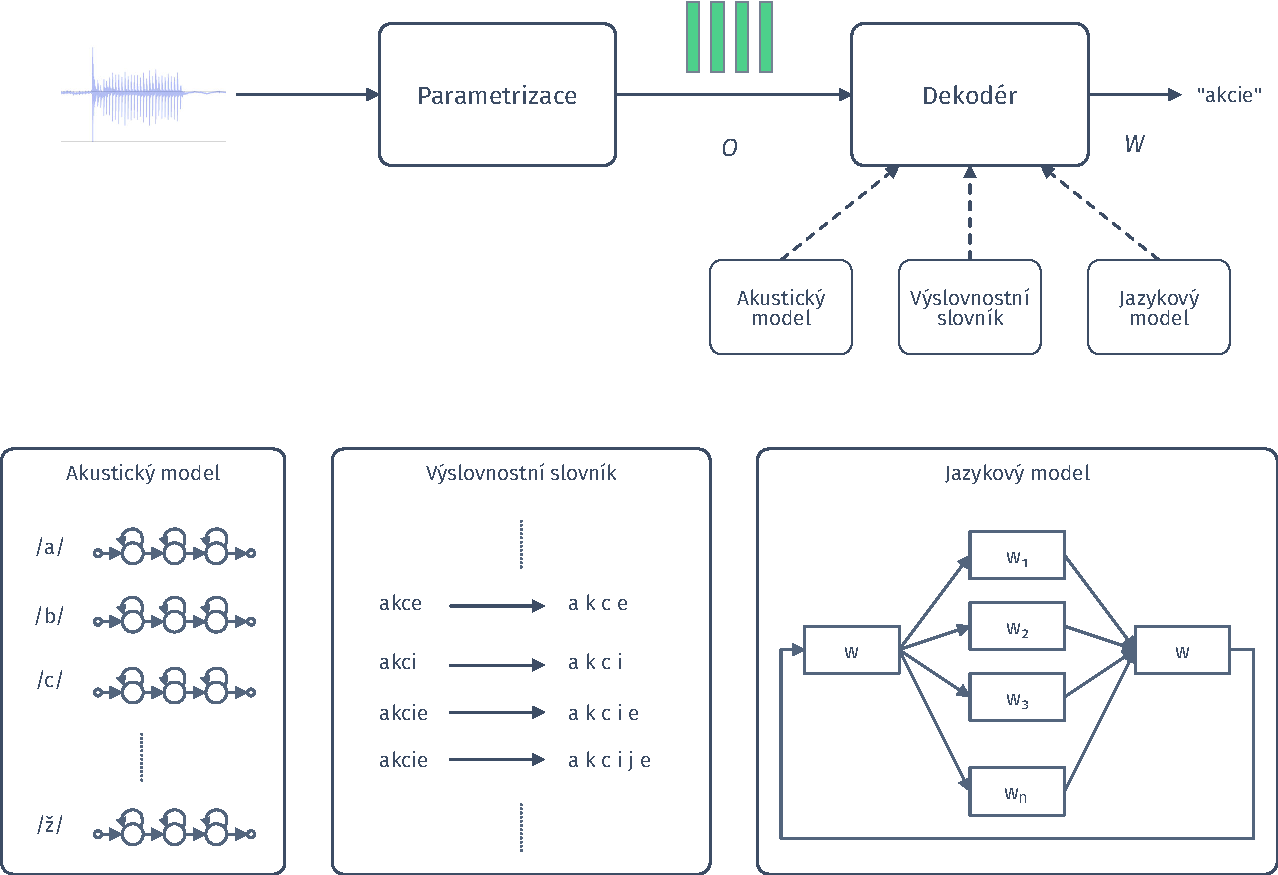
\includegraphics[width=0.9\textwidth]{./ch4-asr/img/decoding.pdf}
  \caption[Schéma ASR systému pracující se statistickou.]{Schéma automatického systému rozpoznávání řeči pracující na statistickém přístupu.}
  \label{fig:asr:decoding}
\end{figure}

\begin{equation}
  \hat{W} = \argmax_W\ P\left(W | \boldsymbol{O}\right).
  \label{eq:asr:decoding}
\end{equation}

\newpage Pomocí Bayesova pravidla je možné podmíněnou pravděpodobnost $P\left(W | \boldsymbol{O}\right)$ vyjádřit jako

\begin{equation}
  P\left(W | \boldsymbol{O}\right) = \frac{P(\boldsymbol{O}|W)P(W)}{P(\boldsymbol{O})},
\end{equation}

\noindent kde podmíněná pravděpodobnost $P(\boldsymbol{O} | W)$ odhaduje sekvenci pozorování $\boldsymbol{O}$ za předpokladu výskytu posloupnosti slov $W$. Tento výpočet je realizován \textbf{akustický modelem} (viz obr. \ref{fig:asr:decoding}). K určení $\hat{W}$ je ještě nezbytné znát pravděpodobnost výskytu požadované posloupnosti slov $P\left(W\right)$, o stanovení této pravděpodobnosti se stará \textbf{jazykový model}. Jelikož pravděpodobnost $P(\boldsymbol{O})$ je z principu nezávislá na sekvenci slov $W$, je možné rovnici (\ref{eq:asr:decoding}) upravit do tvaru

\begin{equation}
  \hat{W} = \argmax_W\ P\left(\boldsymbol{O} | W\right)P(W).
  \label{eq:asr:decoding:generic}
\end{equation}

Takto upravená rovnice představuje obecné pravidlo dekódování a její členy reprezentují základní stavební prvky ASR systému. Pro doplnění je nutné dodat, že \textbf{slovník} obsahuje seznam všech slov, se kterými je systém schopen pracovat. Tento seznam jobsahuje rovněž jejich fonetickou transkripci. Všechny tyto části jsou součástí \textbf{dekodéru}, který realizuje prohledávací strategii. V následujícím textu budou jednotlivé stavební prvky ASR systému popsány podrobněji.

% !TEX root = ../thesis.tex
\section{Parametrizace řečového signálu}
\label{chap:asr:parametrization}

Stejně jako v mnoha jiných odvětvích, i při rozpoznávání řeči je v mnoha případech inspirací člověk. Pro získání sekvence pozorování (příznaků) vycházíme z \textbf{modelování produkce řeči} a \textbf{modelování procesu slyšení}.

\subsection{Modelování produkce řeči}
\label{chap:asr:parametrization:production}

Cílem modelování produkce řeči je nalezení matematických vztahů, které poslouží k~reprezentaci fyzikálních dějů spojených s produkcí řeči. Základem je parametrizační technika \textbf{lineárního prediktivního kódování}, známá pod anglickou zkratkou LPC\footnote{Linear Predictive Coding} \cite{Benesty2007}. Vychází z představy, že hlasové ústrojí člověka je schopno vytvářet tři různé typy řečových zvuků:

\begin{itemize}
  \item \textit{samohlásky} - ty se řadí mezi znělé typy zvuků produkované periodickým buzením vznikajícím pulsy vzduchu, které jsou produkovány hlasivkami;
  \item \textit{frikativy} (např. $/f/$\footnote{Zápis $/f/$ symbolizuje foném, což je akustická reprezentace písmene, \textit{f}. Konkrétní zápisy se mohou lišit podle použité fonetické abecedy. V Čechách se nejčastěji používá abeceda $SAMPA$ či $Z\check{C}FA$.}) - někdy nazývané jako třené souhlásky, protože vznikají třením vydechovaného proudu vzduchu o překážku, kterou mouhou být například zuby nebo jazyk, v některém místě hlasového ústrojí;
  \item \textit{explozivy} (např. $/b/$, $/p/$ ap.) - také nazývané jako souhlásky výbuchové, se tvoří úplným uzavřením vydechovaného proudu vzduchu pomocí artikulačních orgánů. To se následně projeví jako krátká pauza (tzv. okluze), po které následuje náhlé jednorázové uvolnění a únik nahromaděného vzduchu (tzv. exploze) \cite{Psutka2006}.
\end{itemize}

Snahou je navrhnout takový model hlasového traktu, který bude dobře popisovat výše zmíněné řečové zvuky. Nesmí se však zapomenout na možnou přílišnou složitost~a nedostatečnou přesnost modelu. Jako ideální se může jevit lineárně časově invariantní model. Bohužel lidskou řeč lze klasifikovat jako kontinuální časově variantní a v~některých situacích dokonce nelineární proces, proto je téměř nemožné jej přesně namodelovat. Pokud však budeme předpokládat, že v konkrétním krátkém časovém úseku zůstává buzení a parametry hlasivkového traktu přibližně konstantní, tak je možné navrhnout lineární časově invariantní model řeči, který je platný pro krátké časové úseky. Tuto podmínku lze považovat za platnou pro intervaly délky od $10$ do $30\ ms$. Odtud také vychází uvažovaná perioda segmentů řeči, zmíněná v úvodu této kapitoly. Pro tyto segmenty je pak možné proces vytváření řeči modelovat pomocí tzv. \textbf{krátkodobého modelu}, který má v krátkých časových intervalech pevné parametry \cite{Holmes2001}.

Odvození obecného diskrétního modelu hlasivkového traktu je založeno na zjednodušeném modelu produkce řeči, jehož struktura je ukázána na obr. \ref{fig:asr:model:speech}. Ten je tvořen třemi dílčími částmi, konkrétně modelem hlasivek, modelem hlasivkového traktu a modelem vyzařovaného zvuku. K odvození a popisu vlastností modelu se využívá výhod Z-transformace \cite{Psutka2006}.

\begin{figure}[hbpt]
  \centering
  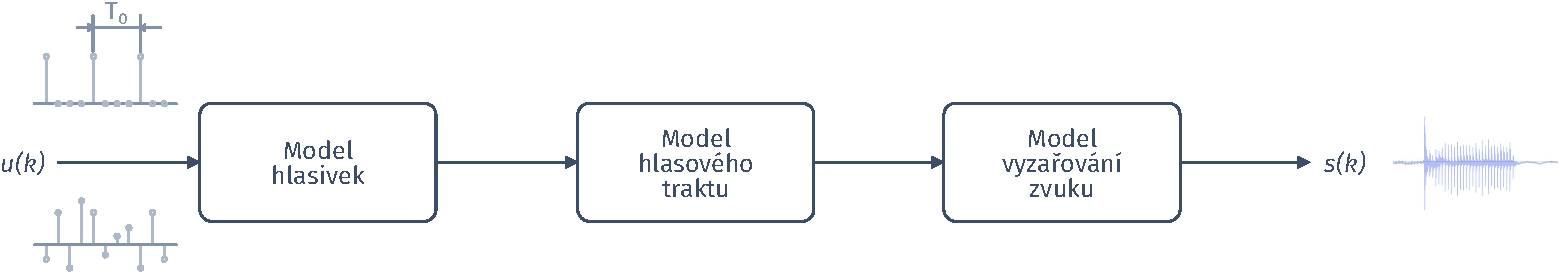
\includegraphics[width=0.9\textwidth]{./ch4-asr/img/speech_model.pdf}
  \caption{Blokové schéma modelu produkce řeči.}
  \label{fig:asr:model:speech}
\end{figure}


Krátkodobý model produkce řeči lze aproximovat celopólovým modelem charakteru filtru $H(z)$ ve tvaru

\begin{equation}
  H(z) = \frac{G}{1 + \sum_{i = 1}^{Q} a_{i} z^{-i}} = \frac{G}{A(z)},
  \label{eq:asr:lpc:generic}
\end{equation}

\noindent kde $G$ představuje celkové zesílení, $Q$ je řád modelu a $a_i$ jsou parametry modelu. Vstupem modelu je buzení $u(k)$ (viz obr. \ref{fig:asr:model:speech}), které je v případě znělých zvuků reprezentováno sledem pulsů s periodou $T_0$\footnote{Perioda základního hlasivkového tónu.} a pro neznělé zvuky je tvořeno náhodným šumem s plochým spektrem. V časové oblasti je pak diskrétní výstupní odezva při fixovaných parametrech hlasového traktu ($10 - 30\ ms$) dána konvolucí buzení a impulzní odezvy krátkodobého modelu. Na základě toho je možné model upravit do podoby znázorněné na obr. \ref{fig:asr:model:speech:excitation}, kde $u(k)$ je buzení a $s(k)$ je výstupní signál s parametry hlasového ústrojí odpovídajícími parametrům $a_i$ celopólového modelu.

\begin{figure}[hbpt]
  \centering
  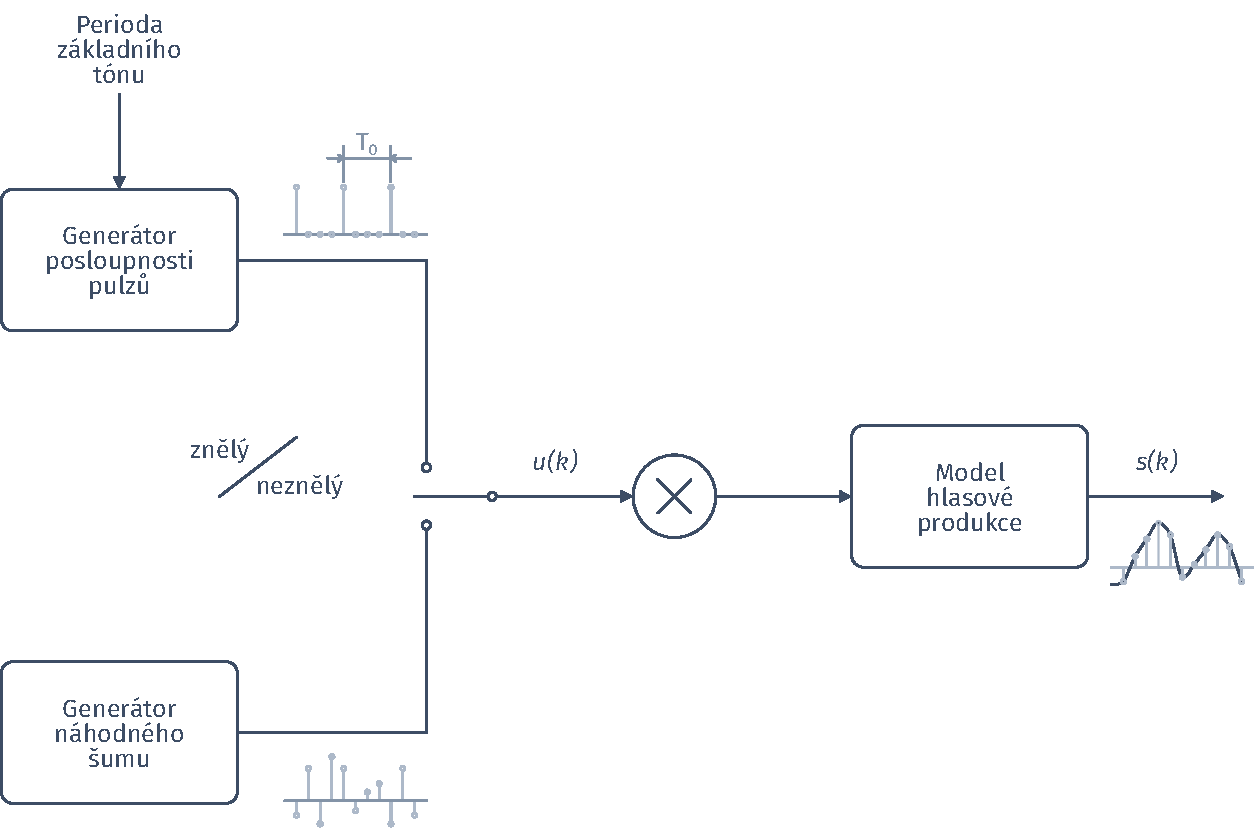
\includegraphics[width=0.9\textwidth]{./ch4-asr/img/speech_process.pdf}
  \caption{Blokové schéma upraveného modelu produkce řeči.}
  \label{fig:asr:model:speech:excitation}
\end{figure}

K odhadu parametrů $a_i$ slouží \textbf{lineární prediktivní analýza}. Odhad probíhá přímo z krátkodobého řečového signálu. Přenosové vlastnosti krátkodobého modelu je možné popsat rovnicí (\ref{eq:asr:lpc:generic}). Myšlenka metody LPC vychází z předpokladu, že vzorek $k$ řečového signálu je možné popsat lineární kombinací $Q$ předchozích vzorků a buzení $u(k)$, což lze matematicky vyjádřit pomocí následující rovnice ve tvaru

\begin{equation}
  s(k) = - \sum_{i = 1}^{Q} a_i s(k-1) + Gu(k).
  \label{eq:asr:lpc:generic:edited}
\end{equation}

\noindent %Z rovnice (\ref{eq:asr:lpc:generic:edited}) 
Je patrné, že se LPC snaží odhadnout parametry modelu $a_i$ a zesílení $G$ pomocí známé reálně naměřené posloupnosti vzorků řeči $s(k)$. K odhadu se používá principu minimalizace kvadratické chyby krátkodobé energie signálu $e\left(k\right)$. Ta je v časové oblasti popsána vztahem

\begin{equation}
  E = \sum_{k} e^2(k) = \sum_{k} \left[ s(k) - s'(k)\right]^2 = \sum_{k} \left( s(k) + \sum_{i = 1}^{Q} a_i s(k-1) + Gu(k) \right),
\end{equation}

\noindent kde $s(k)$ jsou vzorky reálného řečového signálu a $s'(k)$ jsou ty predikované LPC filtrem. Pro nalezení minimální hodnoty krátkodobé chyby predikce $E$ pro konkrétní analyzovaný segment, je použita metoda nejmenších čtverců. K výpočtu konkrétních koeficientů modelu $a_i$ je možné použít rekurzivního Durbinova algoritmu \cite{Holmes2001}.

Další možností jak modelovat hlasový trakt je využít popis pomocí \textbf{kepstrálních koeficientů lineární predikce} $c\left(k\right)$. Kepstrum k-tého mikrosegmentu řečového signálu $s\left(k\right)$ je definováno vztahem % (\ref{eq:asr:lpc:cepstrum:generic}), 


\begin{equation}
  c(k) = \mathcal{F}^{-1}\left\{\log\left| \mathcal{F}\left\{s(k)\right\} \right|\right\}.
  \label{eq:asr:lpc:cepstrum:generic}
\end{equation}

\noindent kde $\mathcal{F}$ představuje operátor diskrétní Fourierovy transformace (DFT) a $\mathcal{F}^{-1}$ reprezentuje inverzní diskrétní Fourierovy transformace (IDFT). Postup výpočtu je znázorněn na obr. \ref{fig:asr:model:speech:cepstrum}.

\begin{figure}[hbpt]
  \centering
  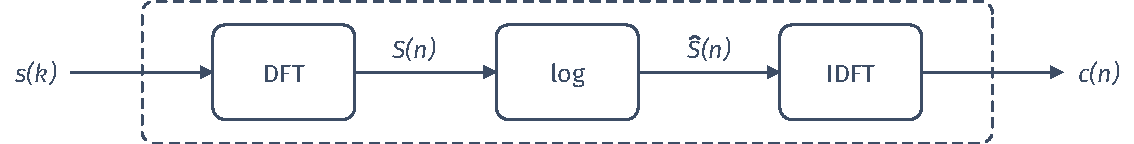
\includegraphics[width=0.9\textwidth]{./ch4-asr/img/cepstrum.pdf}
  \caption{Blokové schéma principu výpočtu kepstra.}
  \label{fig:asr:model:speech:cepstrum}
\end{figure}

Pro získání kepstrálních koeficientů lineární predikce lze využít vztah (\ref{eq:asr:lpc:generic}), který po zlogaritmování přejde do tvaru

\begin{equation}
  \log H(z) = \log \left( \frac{G}{A(z)} \right).
  \label{eq:asr:lpc:cepstrum}
\end{equation}

\noindent Člen $A(z)$ je polynomem proměnné $z^{-1}$ řádu $Q$. Pokud všechny jeho kořeny leží uvnitř jednotkové kružnice, tak lze aplikovat Taylorův rozvoj a vztah (\ref{eq:asr:lpc:cepstrum}), tedy lze zapsat jako

\begin{equation}
  \log \left( \frac{G}{A(z)} \right) = c(0) + c(1)z^{-1} + \dots = \sum_{k=0}^{\infty} c(k)z^{-k},
  \label{eq:asr:lpc:cepstrum:taylor}
\end{equation}

\noindent kde $c(k)$ jsou tzv. kepstrální koeficienty LPC. Po zderivování obou stran rovnice přejde vztah (\ref{eq:asr:lpc:cepstrum:taylor}) do tvaru

\begin{equation}
  - \sum_{i=1}^{Q} ia_iz^{-i} = \left( \sum_{k=0}^{\infty} kc(k)z^{-k} \right)\left( \sum_{i=0}^{Q} a_iz^{-i}\right).
  \label{eq:asr:lpc:cepstrum:deriv}
\end{equation}

\noindent Jestliže se $a_i = 1$, pak lze po roznásobení pravé strany rovnice (\ref{eq:asr:lpc:cepstrum:deriv}) a po následném porovnání členů u stejných mocnin proměnné $z$ zapsat vztahy pro výpočet kepstrálních koeficientů LPC ve tvaru

\begin{align}
  \begin{split}
    c(1) &= -a_1, \\
    c(k) &=
    \begin{cases}
      - a_k - \sum_{i=1}^{k-1} \left(\frac{i}{k}\right) c(i) a_{k-1},  & \quad \text{pro } 2 \leq k \leq Q, \\
      - \sum_{i=1}^{Q} \left(\frac{k - i}{k}\right) c(k-i) a_i,  & \quad \text{pro } k = Q + 1, Q + 2, \dots \quad ,
    \end{cases}
  \end{split}
  \label{eq:asr:lpc:cepstrum:coef}
\end{align}

\noindent kde $k = 1, 2, \dots , Q^{*}$. $Q^{*}$ je počet kepstrálních koeficientů pro které musí platit $Q^{*} \geq Q$. Kepstrální koeficienty LPC jsou vztaženy ke spektrální obálce mikrosegmentu řeči odvozené LPC analýzou. 

Spektrální obálku je následně možné získat z rovnice (\ref{eq:asr:lpc:generic}) dosazením $z = e^{j\omega}$. Pro uspokojivou reprezentaci se tradičně volí $Q$ v rozmezí $7-15$ v závislosti na spektrální šířce přenášeného pásma a požadované přesnosti aproximace. Z toho plyne, že pro popis mikrosegmentu řeči by mohl být dostačující příznakový vektor o $15$ koeficientech.

\subsection{Modelování procesu slyšení}
\label{chap:asr:parametrization:hearing}

Zvuk představuje mechanické vlnění hmotných částic, které se šíří v plynném, kapaném nebo tuhém prostředí. Z fyziologického pohledu je však zvuk považován pouze za slyšitelné vlnění. To je takové, které je schopno vnímat sluchové ústrojí člověka. Zpravidla se jedná o frekvence $16\ Hz - 20\ kHz$. Pro každého člověka je ale toto rozmezí individuální a mění se s věkem. S přibývajícím věkem a sluchovou zátěží klesá hlavně horní mezní kmitočet \cite{Psutka2006}.

To, zda je člověk schopen daný zvuk slyšet, však není závislé pouze na frekvenci zvuku. Velmi podstatná je i intenzita zvuku, která se rovná energii zvukového vlnění, která projde za jednotku času jednotkovou plochou kolmou ke směru šíření vln. Zároveň je úměrná akustickému tlaku zvukové vlny, tj. tlaku, kterým zvukové vlny působí na nějakou překážku. V případě člověka lze překážkou chápat ušní bubínek. Závislost mezi intenzitou zvuku $I\ \left[Wm^{-2}\right]$ a akustickým tlakem $p\ \left[Pa\right]$ je vyjádřen vztahem

\begin{equation}
  I = \frac{p^{2}}{z},
  \label{eq:asr:mfcc:intesity}
\end{equation}

\noindent kde $z$ je měrná akustická impedance prostředí, kterým se zvuk šíří. Lidské ucho je schopno vnímat akustický tlak v rozsahu od $2\cdot10^{-5}$ až $2\cdot10^{2}\ Pa$, tj. v rozsahu sedmi řádů. Z praktického důvodu se tedy používá logaritmické stupnice. K vyjadřování pak slouží logaritmus poměru uvažované veličiny a mezinárodně normované referenční hodnoty téže veličiny \cite{Psutka2006}. Hladina intenzity $L_{I}$ je pak definována vztahem

\begin{equation}
  L_{I} = 10\log_{10}\frac{I}{I_{0}},
  \label{eq:asr:mfcc:intesity:level}
\end{equation}

\noindent kde $I$ představuje intenzitu zvuku a $I_{0} = 10^{-12}\ Wm^{-2}$ referenční hodnotu intenzity. Pro hladinu akustického tlaku platí

\begin{equation}
  L_{p} = 20\log_{10}\frac{p}{p_{0}},
  \label{eq:asr:mfcc:pressure:level}
\end{equation}

\noindent kde $p$ je akustický tlak a $p_{0} = 2\cdot10^{-5}\ Pa$ je referenční hodnota akustického tlaku. Hodnoty veličin $L_{I}$ a $L_{p}$ jsou obvykle udávány v decibelech. %$\left[dB\right]$.

Důležitým pojmem je pak \textbf{práh slyšitelnosti}, který představuje minimální intenzitu zvuku potřebnou k tomu, aby jej šlověk mohl slyšet, viz obr. \ref{fig:asr:mfcc:acoustic:characteristic}. Tento práh je zcela subjektivní a je závislý na frekvenci. Obecně je lidský sluch nejcitlivější na frekvence $3 - 4\ kHz$. Směrem k nižším i vyšším kmitočtům citlivost sluchu klesá. \textbf{Práh bolesti} představuje horní mez intenzity sluchového pole (viz obr. \ref{fig:asr:mfcc:acoustic:characteristic}), při níž již posluchač pociťuje bolest. Překročení této meze může vést k poškození sluchu \cite{Holmes2001}.

\begin{figure}[hbpt]
  \centering
  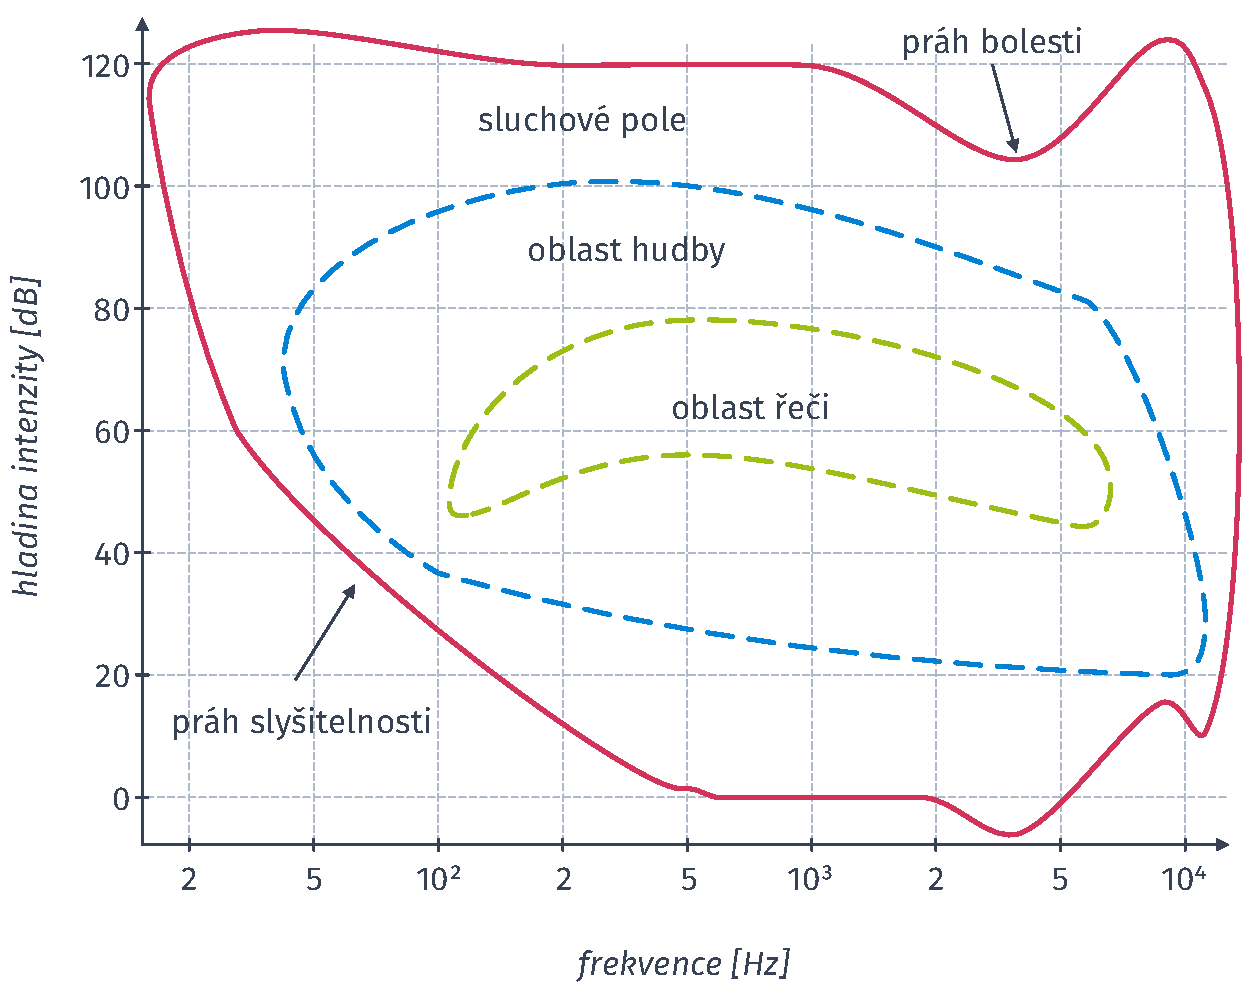
\includegraphics[width=0.75\textwidth]{./ch4-asr/img/listening_perception.pdf}
  \caption[Charakteristické oblasti vnímání akustického signálu.]{Charakteristické oblasti vnímání akustického signálu lidským sluchem. $L_p = 20log(p/p0),\ p0 = 2\bullet10^{–5}\ Pa$.}
  \label{fig:asr:mfcc:acoustic:characteristic}
\end{figure}

Hlasitost zvuku je závislost intenzity na frekvenci a je zcela subjektivní pocit, kterým člověk posuzuje intenzitu daného zvuku. Na obr. \ref{fig:asr:mfcc:acoustic:levels} jsou vyznačeny hladiny hlasitosti, které vznikly spojením bodů ve sluchovém poli (obr. \ref{fig:asr:mfcc:acoustic:characteristic}), odpovídající tónům, které člověk vnímá stejně hlasitě. Z křivek je patrné, že subjektivní hlasitost se mění s frekvencí zvuku. Zvuky s nižší frekvencí vnímáme méně hlasitěji než zvuky s vyšší frekvencí, zejména pak zvuky v rozmezí $3 - 4\ kHz$ \cite{Psutka2006}.

\begin{figure}[hbpt]
  \centering
  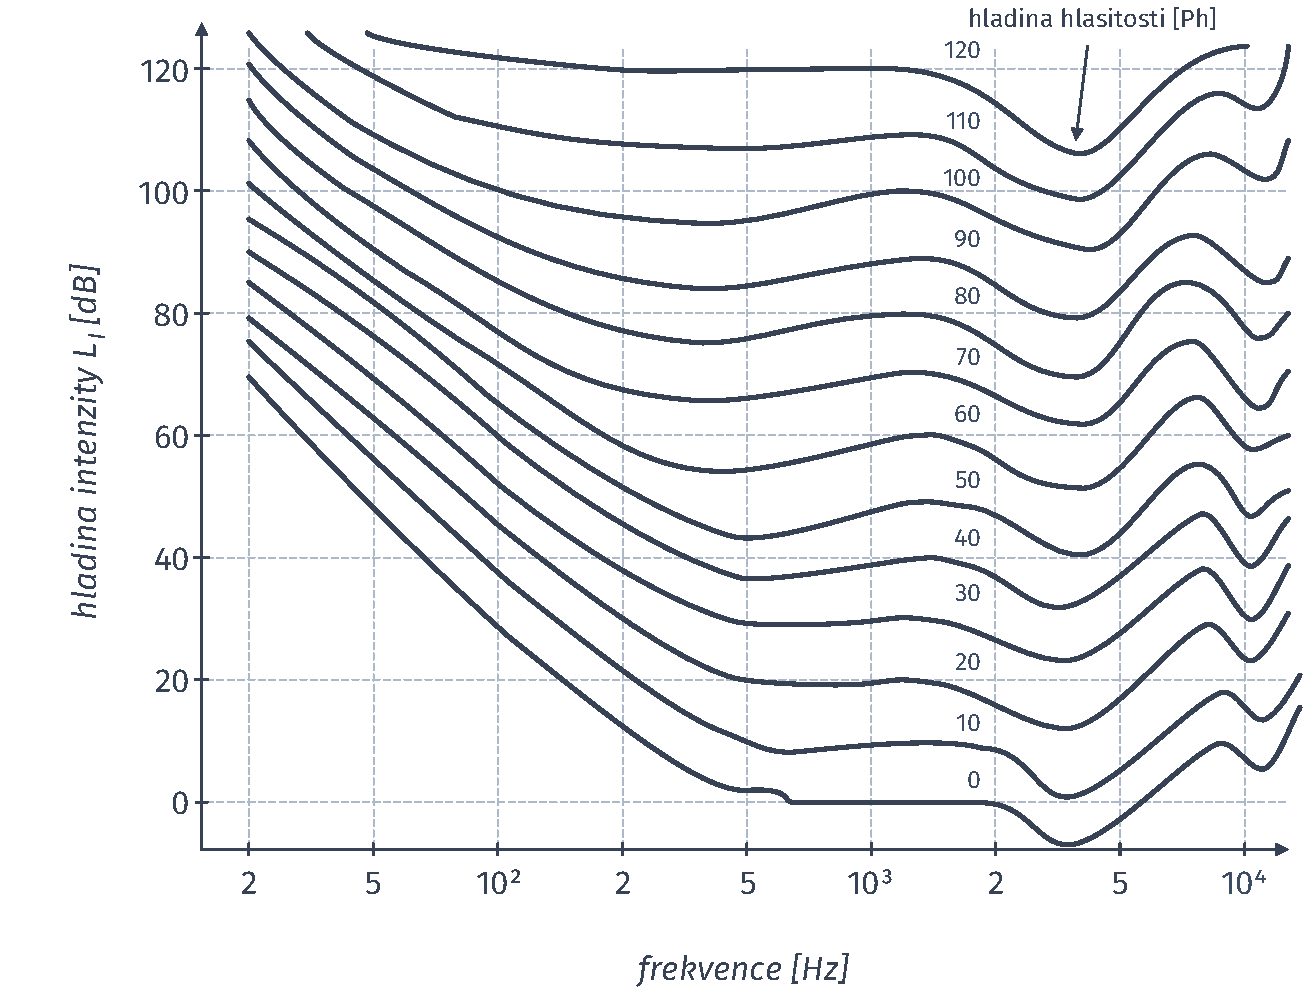
\includegraphics[width=0.75\textwidth]{./ch4-asr/img/listening_levels.pdf}
  \caption[Křívky stejné hlasitosti.]{Křivky stejné hlasitosti. $L_p = 20log(p/p0),\ p0 = 2\bullet10^{–5}\ Pa$.}
  \label{fig:asr:mfcc:acoustic:levels}
\end{figure}

Principem modelování procesu slyšení je postižení kompenzace nelineárního vnímání frekvencí lidským sluchem a respektování maskování zvuků včetně tzv. kritických pásem slyšení. Maskování zvuků je přirozená vlastnost lidského sluchu. Rozumí se jím jev, kdy je vnímání jednoho zvuku ovlivněno přítomností jiného zvuku. Jinými slovy lze říci, že přítomnost jednoho zvuku zvyšuje práh slyšitelnosti pro jiný zvuk. Ten buď zní současně nebo s drobným časovým odstupem od toho prvního. Tento jev je jakýsi \uv{psychologický filtr}, který ignoruje veškerý šum ležící mimo určité kritické pásmo slyšení. Šířka kritického pásma je přitom závislá na frekvenci poslouchaného tónu. Často užívanými metodami pro modelování procesu slyšení jsou \textbf{melovská kepstrální filtrace} a \textbf{perceptivní lineární prediktivní analýza}.

\subsubsection{Melovské kepstrální koeficienty}

Metoda melovských frekvenčních kepstrálních koeficientů (MFCC) se snaží respektovat výše zmíněné vlastnosti lidského sluchu, především se snaží dodržet kritická pásma slyšení a vliv subjektivního vnímání výšky tónů.

Základem MFCC je využití banky filtrů a lineárního rozložení frekvencí v tzv. \textbf{melovské frekvenční škále} definované vztahem

\begin{equation}
  f_m = 2595 \log \left(1 + \frac{f}{700}\right),
  \label{eq:asr:mfcc:melscale}
\end{equation}

\noindent kde $f \left[Hz\right]$ je frekvence v lineární škále a $f_m \left[mel\right]$ je odpovídající frekvence v melovské stupnici. Melovský filtr má trojúhelníkový tvar. Banka obsahuje $M^{*}$ filtrů rozmístěných lineárně v melovských frekvenčních souřadnicích, a to tak, že dva sousední filtry se navzájem o polovinu překrývají. Pro střední frekvence jednotlivých filtrů $b_{m,i}$ v melovské škále platí vztah

\begin{equation}
  b_{m,i} = b_{m,i-1} + \Delta_{m},
  \label{eq:asr:mfcc:freq}
\end{equation}

\noindent kde $b_{m, 0} = 0\ mel$, $i = 1, 2,\ \dots\ , M^{*}$, a $\Delta_m = B_{m,w} / (M^{*} + 1)$, kde $B_{m,w}$ je celková šířka pásma v melovské škále. Ukázka banky filtrů v této škále je znázorněna na obr. \ref{fig:asr:mfcc:bank:mel}. Pro výpočet odezvy filtrů je však nezbytné přepočítat všechny koeficienty FFT do melovské frekvenční škály.

\begin{figure}[hbpt]
  \centering
  \includegraphics[width=0.9\textwidth]{./ch4-asr/img/filter_bank-mel.pdf}
  \caption{Rozložení banky trojúhelníkových filtrů v melovské frekvenční škále.}
  \label{fig:asr:mfcc:bank:mel}
\end{figure}

\noindent Vhodnější je vyjádření trojúhelníkových filtrů ve frekvenční škále s měřítkem v herzích. K přepočtu středních frekvencí $b_{m,i}$ se využívá inverzního vztahu k (\ref{eq:asr:mfcc:melscale}), tedy

\begin{equation}
  f = 700 \left[ \exp\left( 0,887.10^{-3} f_m \right) - 1 \right].
  \label{eq:asr:mfcc:melscale:inverse}
\end{equation}

\noindent Střední frekvence $b_i$ jednotlivých filtrů jsou vyjádřené také v herzích. Na rozdíl od popisu v melovské škále jsou filtry rozmístěny nelineárně napříč celým analyzovaným spektrem, viz obr. \ref{fig:asr:mfcc:bank:hz}.

\begin{figure}[hbpt]
  \centering
  \includegraphics[width=0.9\textwidth]{./ch4-asr/img/filter_bank-hz.pdf}
  \caption{Rozložení banky trojúhelníkových filtrů ve frekvenční škále.}
  \label{fig:asr:mfcc:bank:hz}
\end{figure}

Na vstup systému jsou postupně přivedeny mikrosegmenty řečového signálu\footnote{Jednotlivé mikrosegmenty byly nejprve předzpracovány , tj. prošly tzv. preemfází. Ta spočívá ve zdůraznění amplitud spektrálních složek řečového signálu s jejich vzrůstající frekvencí \cite{Psutka2006}.} $s\left(k\right)$ o konstantní délce a pro ně jsou určeny odpovídající koeficienty $c\left(k\right)$. Pro jednotlivé mikrosegmenty je pomocí FFT vypočteno amplitudové spektrum $\left| S(f) \right|$ a následuje klíčová část celého procesu, melovská filtrace. Odezvy filtrů ve frekvenční oblasti lze stanovit pomocí vztahu

\begin{equation}
  y_m(i) = \sum_{f=b_{i-1}}^{b_{i+1}} \left| S(f) \right| u\left(f, i\right),  \quad i = 1, 2,\ \dots\ ,M^{*},
  \label{eq:asr:mfcc:freq:responce}
\end{equation}

\noindent kde frekvence $f$ jsou vybírány ze souboru frekvencí využívaných při FFT výpočtu a $u(f, i)$ je vyjádření konkrétního trojúhelníkového filtru $i$. Průchod filtrem tedy znamená, že každý koeficient FFT je násoben odpovídajícím ziskem filtru a výsledky jsou pro příslušné filtry akumulovány. Logaritmováním akumulovaných koeficientů $y_{m}(i)$ je realizován převod do kepstrální oblasti. Tento krok příznivě omezí dynamiku signálu \cite{Benesty2007}. Posledním krokem při výpočtu melovských kepstrálních koeficientů $\left\{c_m\left(j\right)\right\}_{j=1}^{M}$ je provedení IDFT podle vztahu (\ref{eq:asr:lpc:cepstrum:generic}). V případě MFCC se ale používá diskrétní kosinová transformace (DCT), protože spektrum je reálné a symetrické. K výpočtu slouží vztah

\begin{equation}
  c_{m}(j) = \sum_{i=1}^{M^{*}} \log y_m(i) \cos\left( \frac{\pi j}{M^{*}}\left(i - 0,5\right) \right) \quad \text{pro}\ j = 0, 1,\ \dots\ ,M,
  \label{eq:asr:mfcc:coef}
\end{equation}

\noindent kde $M^{*}$ je počet pásem melovkého pásmového filtru a $M$ je počet melovských kepstrálních koeficientů. Počet těchto koeficientů $M$ se volí podstatně menší než je počet pásem melovského pásmového filtru $M^{*}$, obvykle se uvažuje prvních $10\ \text{až}\ 13$ koeficientů. Velmi často se také používá $1.$ a $2.$ z těchto koeficientů, protože svým způsobem zohledňují dynamickou složku řeči.

\subsubsection{Perceptivní lineární prediktivní analýza}

Stejně jako MFCC, tak také i \textbf{perceptivní lineární prediktivní analýza (PLP)} vychází z lidského vnímání a slyšení zvuků. Snaha je postihnout z psychofyziky slyšení zejména kritická pásma spektrální citlivosti, vztah mezi intenzitou a vnímáním hlasitosti a také křivky stejné hlasitosti \cite{Psutka2006}. PLP podobně jako LPC pak aproximuje získané sluchové spektrum koeficienty autoregresního celopólového modelu.

Prvním krokem PLP analýzy je \textbf{výpočet výkonového spektra řečového signálu}. Pro konkrétní předzpracovaný\footnote{Ještě před výpočtem je stejně jako u MFCC aplikována preemfáze.} mikrosegment řečového signálu $s(k)$ aplikujeme DFT. Krátkodobé spektrum je pak definováno vztahem

\begin{equation}
  P\left(\omega\right) = \left| S\left(\omega\right) \right|^{2} = \left[Re\ S\left(\omega\right)\right]^2 + \left[Im\ S\left( \omega \right) \right]^2.
  \label{eq:asr:plp:spectr}
\end{equation}

\noindent Poté následuje kompenzace nelineárního vnímání změn ve výšce zvuku. Vnímání je logaritmické, proto je nutné provést nelineární transformaci frekvenční osy pomocí vzorce

\begin{equation}
  \Omega\left(\omega\right) = 6 \ln \left( \frac{\omega}{1200\pi} + \sqrt{\left(\frac{\omega}{1200\pi}\right)^2 + 1} \right),
  \label{eq:asr:plp:transform}
\end{equation}

\noindent kde $\omega = 2\pi f\ \left[rad/s\right]$ a $\Omega\left(\omega\right)\ \left[Bark\right]$.

Zahrnutí kritických pásem slyšení (tzv. maskování zvuku) je realizováno navržením vhodného filtru typu pásmová propust šířky jednoho kritického pásma. Stejně jako v případě MFCC se jedná o banku filtrů, kde na sebe jednotlivé filtry ve frekvenční oblasti navazují.
%Na Barkově frekvenční ose (viz (\ref{eq:asr:plp:transform})) mají všechny filtry šířku $1$ a jsou lineárně rozmístěny.
Na obr. \ref{fig:asr:plp:filter} je zobrazen průběh jednoho takového filtru. Filtr má strmost $+20\ dB/Bark$ směrem k nižším frekvencím a $-50\ dB/Bark$ směrem k vyšším frekvencím.

\begin{figure}[hbpt]
  \centering
  \includegraphics[width=0.5\textwidth]{./ch4-asr/img/plp_filter.pdf}
  \caption{Ukázka filtru umístěného na Barkově frekvenční ose.}
  \label{fig:asr:plp:filter}
\end{figure}

\newpage \noindent Na Barkově frekvenční ose mají jednotlivé filtry šířku $1$ a jsou podél ní lineárně rozmístěny viz obr. \ref{fig:asr:plp:bank},
% Rozmístění filtrů na Barkově frekvenční ose je pak znázorněno na obr. \ref{fig:asr:plp:bank}.

\begin{figure}[hbpt]
  \centering
  \includegraphics[width=0.9\textwidth]{./ch4-asr/img/plp-bank.pdf}
  \caption{Rozmístění filtrů na Barkově frekvenční ose.}
  \label{fig:asr:plp:bank}
\end{figure}

Jelikož člověk vnímá intenzitu zvuku v závislosti na frekvenci, tak je potřeba provést \textbf{přizpůsobení křivkám stejné hlasitosti}. Na začátku je důležité definovat referenční hlasitost, tj. hlasitost, na kterou bude normalizována. Obvykle se volí $40\ Ph$ \cite{Psutka2006}, což přibližně odpovídá hlasitosti běžné řeči. K normalizaci je použit inverzní filtr popsaný vztahem

\begin{equation}
  E\left(\omega\right) = K \frac{\omega^4\left(\omega^2 + 56,9 \cdot 10^6\right)}{\left(\omega^2 + 6,3 \cdot 10^6\right)^2\left(\omega^2 + 379,4 \cdot 10^6\right)\left(\omega^6 + 9,6 \cdot 10^{26}\right)},
  \label{eq:asr:plp:filter}
\end{equation}

\noindent kde $\omega = 2\pi f$ a $K$ je konstanta nastavená podle požadovaného zesílení. Přizpůsobení křivce stejné hlasitosti je pak možné například přenásobením celého výkonového spektra mikrosegmentů podle vztahu

\begin{equation}
  P'\left(\omega\right) = E\left(\omega\right)P\left(\omega\right),
  \label{eq:asr:plp:filter:application1}
\end{equation}

\noindent kde $P'\left(\omega\right)$ je spektrum transformované na stejnou hlasitost. Případně lze upravit tvar jednotlivých filtrů pomocí vztahu

\begin{equation}
  \Phi\left(\omega, i\right) = E\left(\omega\right)\Psi\left(\omega - \omega_i, i\right),
  \label{eq:asr:plp:filter:application2}
\end{equation}

\noindent kde $\Phi\left(\omega, i\right)$ je nový tvar filtru $i$ v závislosti na frekvenci $\omega$, $\Psi\left(\omega - \omega_i, i\right)$ je odezva filtru $i$ se středovou frekvencí $\omega_i$.

Po přizpůsobení následuje \textbf{výpočet energie jednotlivých filtrů}, to je obdobné jako u MFCC. Výpočet se provádí pro jednotlivé filtry a výsledky se pak sčítají. Matematicky to je zapsáno vztahem

\begin{equation}
  \zeta_m = \sum_{\Omega = \Omega_m - 2,5}^{\Omega_m + 1,3} P\left(\Omega\right)\Phi\left(\Omega, m\right), \quad\ m=1, 2,\ \dots\ M - 2,
  \label{eq:asr:plp:energy}
\end{equation}

\noindent kde $M$ je počet použitých filtrů (kritických pásem).

Dalším krokem výpočtu je uplatnění \textbf{\uv{zákona slyšení}}. Ten popisuje závislost mezi intenzitou a vnímanou hlasitostí. Na energie $\zeta_m$ je aplikována nelineární transformace vyjádřena vztahem

\begin{equation}
  \xi_m = \left(\zeta_m\right)^{0,3}, \quad\ m = 1, 2,\ \dots\ M-2,
  \label{eq:asr:plp:energy:transform}
\end{equation}

\noindent kde $M$ je opět počet filtrů. Díky této operaci dojde také k redukci proměnlivosti \uv{výstupů} kritických pásmových filtrů a výsledný hledaný celopólový model může být relativně nízkého řádu.

Finálním krokem je \textbf{aproximace celopólového modelu}. Ta vychází z výpočtu koeficientů celopólového modelu metody LPC, kde je model popsán vztahem (\ref{eq:asr:lpc:generic:edited}). Pro chybu predikce pak platí

\begin{equation}
  e\left(k\right) = \sum_{k} \left(s\left(k\right) + \sum_{i=1}^{Q} a_i s\left(k - i\right)\right).
  \label{eq:asr:plp:error}
\end{equation}

\noindent Aplikací Z-transformace a uvážením rovnice (\ref{eq:asr:lpc:generic}), je možné vztah (\ref{eq:asr:plp:error}) upravit do tvaru

\begin{equation}
  E\left(z\right) = \left[1 + \sum_{i=1}^{Q} a_i z^{-i}\right] S\left(z\right) = A\left(z\right)S\left(z\right),
  \label{eq:asr:plp:error:transform}
\end{equation}

\noindent kde $A\left(z\right)$ je inverzní filtr a $E\left(z\right)$, resp. $S\left(z\right)$ jsou získané Z-transformací $e\left(k\right)$, resp. $s\left(k\right)$. Celkovou chybu predikce je pak možné vyjádřit vztahem

\begin{equation}
  E\left(z\right) = \frac{1}{2\pi} \int_{-\pi}^{\pi} P\left(\omega\right) A\left(e^{j\omega}\right) A\left(e^{-j\omega}\right)d\omega,
  \label{eq:asr:plp:error:final}
\end{equation}

\noindent kde $P\left(\omega\right)$ je vypočtené výkonové spektrum. Podobně jako u LPC hledané řešení odpovídá hodnotám, pro něž je celková chyba autokorelační funkce $R\left(i\right)$ minimální. Pro konečný počet známých frekvencí je tato funkce definována vztahem

\begin{equation}
  R\left(i\right) = \frac{1}{N} \sum_{n=0}^{N-1} P\left(\omega_n\right) \cos\left(i\omega_n\right),
  \label{eq:asr:plp:error:solution}
\end{equation}

\noindent kde $i = 0,\ \dots\ Q$, $Q$ je řád autoregresního modelu a $N$ je počet bodů spektrální charakteristiky. Frekvence $\omega_n$ jsou ty, pro které jsou známé spektrální hodnoty. Pro dobrou aproximaci se volí $Q = 5$ \cite{Benesty2007}. \textbf{Výpočet kepstrálních koeficientů PLP} lze pak pro známé hodnoty $R\left(i\right)$, podobně jako u LPC, určit Durbinovým algoritmem. Nalezené koeficienty lze využít jako příznaky při návrhu parametrizátoru řeči
\cite{Holmes2001}.

K vytvoření parametrizátoru je možné použít libovolnou výše popsanou metodu. %metodu představenou v \ref{chap:asr:parametrization:production} a \ref{chap:asr:parametrization:hearing}. 
V současnosti ale převládají metody postavené na principu fungování lidského sluchu, protože amplifikují podstatnou informaci zakódovanou v řeči.

% !TEX root = ../thesis.tex
\section{Akustické modelování}
\label{chap:asr:acoustic}

Akustický model představuje v rovnici (\ref{eq:asr:decoding:generic}) podmíněnou pravděpodobnost $p(O|W)$. Úkolem akustického modelu je poskytnout co nejpřesnější odhad této pravděpodobnosti pro libovolnou posloupnost vektorů příznaků $O = \left\{o_1 o_2\ \dots\ o_T\right\}$. Velmi vhodným způsobem modelování řeči se ukázalo být využití tzv. \textbf{skrytých Markovových modelů (HMM)}. Ty vycházejí z principu vytváření řeči člověkem. V průběhu produkce řeči se hlasové ústrojí nachází vždy v krátkém časovém úseku nachází v jednom z konečného počtu konfiguracé. V tomto mikrosegmentu je pak hlasovým ústrojím generovám krátký signál, který zavisí na aktuální konfiguraci. Tento vyprodukovaný zvuk je metodami (popsanými v \ref{chap:asr:parametrization}) převeden na vektor příznaků $O$.

Skrytý Markovův model je model stochastického procesu. Na ten je možné nahlížet jako na pravděpodobnostní konečný automat, který v diskrétních časových okamžicích generuje náhodnou posloupnost vektorů příznaků $O = \left\{o_1 o_2\ \dots\ o_T\right\}$. Model v každém časovém kroku změní stav svůj $s_j$ podle předem daných pravděpodobností přechodu $a_{ij}$. Přechod ze stavu $s_i$ do stavu $s_j$ má za následek vygenerování výstupního vektoru pozorování $o_t$ a to podle rozdělení výstpní pravděpodobnosti $b_j\left(o_t\right)$ příslušné k tomuto stavu \cite{Psutka2006}.

Podmínění pravděpodobnost přechodu $a_{ij}$ určuje, s jakou pravděpodobností přechází model ze stavu $i$ v čase $t$, do stavu $j$ v čase $t+1$. Platí tedy

\begin{equation}
  a_{ij} = p\left(s\left(t+1\right)=s_j|s\left(t\right)=s_i\right),
  \label{eq:asr:acoustic:conditional}
\end{equation}

\noindent kde $s\left(t\right)$ je stav modelu v čase $t$. Další podmínkou je, že pro všechny stavy $i$, $i=1,2,\dots\,N$, platí

\begin{equation}
  \sum_{j=1}^{N} a_{ij} = 1.
  \label{eq:asr:acoustic:state:condition}
\end{equation}

\noindent Funkce rozdělení výstupní pravděpodobnosti $b_j\left(o_t\right)$ popisují rozdělení pravděpodobnosti pozorování $o_t$ produkovaného ve stavu $s_j$ v čase $t$. Pro tuto funkci platí

\begin{equation}
  b_j\left(o_t\right) = P\left(o_t|s\left(t\right)=s\right),
  \label{eq:asr:acoustic:state:output}
\end{equation}

\noindent kde $P$ značí pravděpodobnost, pro kterou u diskrétních rozdělení platí

\begin{equation}
  \sum_o b_j\left(o\right) = 1.
  \label{eq:asr:acoustic:state:output:condition:discrete}
\end{equation}

\noindent Pro spojité rozdělení pak alternativně

\begin{equation}
  \int_o b_j\left(o\right)do = 1.
  \label{eq:asr:acoustic:state:output:condition:continous}
\end{equation}

\noindent V obou případech to platí pro všechny stavy HMM, které mohou generovat výstupní vektor.

Rozdělení výstupní pravděpodobnosti musí být při modelování řečových zvuků dostatečně specifické, aby bylo možné od sebe oddělit různé zvuky, a zároveň dostatečně robustní, aby zahrnulo značnou variabilitu řečového signálu. Toto rozdělení je možné modelovat

\begin{itemize}
  \item spojitým normálním rozdělením se směsí hustotních funkcí,
  \item neuronovými sítěmi.
\end{itemize}

\subsection{Struktura skrytého Markovova modelu}
\label{chap:asr:acoustic:HMM}

Z pohledu rozpoznávání řeči se nejčastěji využívá tzv. levo-pravá struktura Markovova modelu. V průběhu let bylo testováno mnoho různých struktur HMM, např. modely s počtem stavů odvozených od průměrné délky slova pro nějž byl model konstruován, až po pevnou strukturu stavů pro každé slovo. Tyto modely sloužily hlavně pro rozpoznávání izolovaných úseků řeči, nejčastěji slov. V současnosti, kdy je většina systémů konstruovaných pro zpracování souvislé řeči a počet slov ve slovníku může přesahovat 1 milion slov, převažují modely odvozené od menších jednotek, než jsou slova. Takovými jednotkami mohou být například fonémy anebo specifičtější trifóny. Trifón je svým způsobem kontextově závislý foném, který bere v potaz svůj levý a pravý kontext, tj. levý a pravý sousední foném. Přepis slova do fonémově, resp. trifónové struktury, lze ukázat na příkladu izolovaného slova \uv{akcie}, které má přepis \uv{\texttt{sil a k c i j e sil}}, v trifónové podobě je pak zápis následující

\begin{verbatim}
  sil sil-a+k a-k+c k-c+i c-i+j i-j+e j-e+sil sil,
\end{verbatim}

\noindent kde \texttt{sil} má význam pauzy před, případně za vyslovenou promluvou slova \uv{akcie}.

Oproti slovním modelům, u fonémů (monofónů), resp. trifónů, bývá struktura relativně jednoduchá a často je vyjádřena $5$ stavovým modelem (znázorněn na obr. \ref{fig:asr:acoustic:hmm}). Jedná se o $5$ stavový levo-pravý Markovův model, jehož první a poslední stav jsou tzv. neemitující. Jejich primární úlohou je zřetězování jednotlivých HMM modelů trifónů (monofónů) do rozsáhlajších modelů, např. slov, vět ap. Při zřetězení se tyto neemitující stavy vypouštějí. Ostatní stavy modelu jsou emitující a vztahují se k nim odpovídající rozdělení pravděpodobnosti $b_j(.)$.

\begin{figure}[hbpt]
  \centering
  \includegraphics[width=0.7\textwidth]{./ch4-asr/img/hmm_structure.pdf}
  \caption{Příklad levo-pravého Markovova modelu trifónu}
  \label{fig:asr:acoustic:hmm}
\end{figure}

Pokud předpokládáme, že posloupnost slov $W$ je modelována zřetězeným skrytým Markovovým modelem $\lambda$, kde dílčí modely odpovídají fonetickým jednotkám, pak je možné určit pravděpodobnost generování posloupnosti $O$ modelem $\lambda$ jako

\begin{equation}
  P\left(O|\lambda\right) = \sum_{\forall S} P\left(O, S| \lambda\right)P\left(S|\lambda\right) = \sum_{\forall S} a_{s\left(0\right)s\left(1\right)} \prod_{t=1}^{T} b_{s\left(t\right)}\left(o_t\right)a_{s\left(t\right)s\left(t+1\right)},
  \label{eq:asr:acoustic:structure:output}
\end{equation}

\noindent kde posloupnost stavů $S = \left\{s\left(0\right), s\left(1\right),\dots, s\left(T+1\right)\right\}$ je chápána tak, že $s\left(0\right)$ je výstpní a $s\left(T+1\right)$ výstupní neemitující stav modelu $\Theta$ dané promluvy \cite{Psutka2006}. Přitom tento model lze značit trojicí

\begin{equation}
  \lambda = \left[\left\{a_{ij}\right\}_{k,s=1}^{I}; \left\{b_s(.)\right\}_{s=1}^{I};\left\{\pi_{s}\right\}_{s=1}^{I}\right],
  \label{eq:asr:acoustic:structure:marking}
\end{equation}

\noindent kde $a_{ij}$ je přechodová a $b_s(.)$ výstupní pravděpodobnost. Dále $\pi_s$ je rozložení pravděpodobnosti počátečního stavu a $I$ je počet stavů modelu.

Přímé vyčíslení pravděpodobnosti $P\left(O|\lambda\right)$ podle vztahu (\ref{eq:asr:acoustic:state:output}) je z hlediska počtu operací často nerealizovatelné, protože se jedná řádově o $2TN^{T}$ operací násobení. Z tohoto důvodu se proto využívá výpočetně efektivnější tzv. \textbf{algoritmus forward-backward (FB)} s přibližně $N^{2}T$ operací násobení.

Při výpočtu odpředu (forward) se určuje pravděpodobnost $\alpha_j\left(t\right)$ definovaná vztahem

\begin{equation}
  \alpha_{j}\left(t\right) = P\left(o_1o_2\dots o_t, s\left(t\right)=s_j|\lambda\right),
  \label{eq:asr:acoustic:structure:forward}
\end{equation}

\noindent pro výpočet odzadu (backward) se určuje pravděpodobnost $\beta_j\left(t\right)$ definována vztahem


\begin{equation}
  \beta_j\left(t\right) = P\left(o_{t+1}o_{t+2}\dots o_T|s\left(t\right)=s_j|\lambda\right).
  \label{eq:asr:acoustic:structure:backward}
\end{equation}

Podle \cite{Psutka2006} lze snadno dokázat, že výsledná pravděpodobnost $P\left(O|\lambda\right)$ může být vyčíslena vztahem

\begin{equation}
  P\left(O|\lambda\right) = \sum_{s=1}^{N} P\left(O, s\left(t\right) = s | \lambda\right) = \sum_{i = 1}^{N} \alpha_{i}\left(t\right)\beta_{i}\left(t\right)
  \label{eq:asr:acoustic:structure:forward-backward}
\end{equation}

\noindent pro $1 \leq t \leq T$.

\subsection{Trénování parametrů HMM s Gausovkými směsmi}
\label{chap:asr:acoustic:GMM}

Volba struktrury skrytého Markovova modelu je spíše expertní úlohou návrhu. Stanovéní hodnot parametrů modelu je uskutečněno trénováním (odhadem, etimací) na základě trénovacích akustických dat a jejich textových anotací (tzv. korpus). Pro trénování parametrů se využívá tzv. Baum-Welchův interativní algoritmus, což je speciální případ EM algoritmu. Více o něm v \cite{Holmes2001}. Pro odhad střední hodnoty $\mu_{sj}$, tj. složky $m$ gaussovské směsi ve stavu $j$ slouží vztah

\begin{equation}
  \hat{\mu}_{jm} = \frac{\sum_{t=1}^{T}\gamma_{jm}\left(t\right)o_t}{\sum_{t=1}^{T}\gamma_{jm}\left(t\right)},
  \label{eq:asr:acoustic:structure:mu}
\end{equation}

\noindent kde $N$ je počet stavů a $M$ počet složek. Také platí $1 \leq j \leq N$ a $1 \leq m \leq M$. Odhad kovarianční matice $C_{jm}$, tj. složky náležící m-té složce gaussovské směsi ve stavu $j$

\begin{equation}
  \hat{C}_{jm} = \frac{\sum_{t=1}^{T} \gamma_{jm}\left(t\right)\left(o_t - \hat{\mu}_{jm}\right)\left(o_t - \hat{\mu}_{jm}\right)^{T}}{\sum_{t=1}^{T}\gamma_j\left(t\right)},
  \label{eq:asr:acoustic:structure:covariant}
\end{equation}

\noindent kde $1 \leq j \leq N$ a $1 \leq m \leq M$. Odhad váhové složky hustotní směsi $c_{jm}$, tj. složky náležící složce $m$ gaussovské směsi ve stavu $j$ se provádí vztahem

\begin{equation}
  \hat{c}_{jm} = \frac{\sum_{t=1}^{T} \gamma_{jm}\left(t\right)}{\sum_{t=1}^{T}\gamma_j\left(t\right)},
  \label{eq:asr:acoustic:structure:weight}
\end{equation}

\noindent kde $1 \leq j \leq N$ a $1 \leq m \leq M$. Přitom $\gamma_{j}\left(t\right)$ představuje přavděpodobnost, že proces generování posloupnosti $O$ je v čase $t$ ve stavu $j$. Pro vyjádření této pravděpodobnosti $\gamma_{j}\left(t\right)$ platí rovnice (\ref{eq:asr:acoustic:structure:forward-backward}). Pro její definování pak platí vztah

\begin{equation}
 \gamma_{j}\left(t\right) = \frac{P\left(O, s\left(t\right)=j|\lambda\right)}{P\left(O|\lambda\right)} = \frac{\alpha_{j}\left(t\right)\beta_{j}\left(t\right)}{P\left(O|\lambda\right)} ,
  \label{eq:asr:acoustic:structure:gamma}
\end{equation}

\noindent kde $j = 1,\dots,N$ a $t = 1, \dots, T$. Pravděpodobnost, že proces generování posloupnosti $O$ je v čase $t$ ve stavu $j$ a generuje složku $m$ gaussovské hustotní směsi

\begin{equation}
  \gamma_{jm}\left(t\right) = \frac{P\left(O, s\left(t\right)=j, m\left(j,t\right)=m|\lambda\right)}{P\left(O|\lambda\right)} = \frac{\alpha_{j}\left(t\right)\beta_{j}\left(t\right)}{P\left(O|\lambda\right)} \frac{c_{jm}\mathcal{N}\left(o_t;\mu_{jm}; C_{jm}\right)}{\sum_{i=1}^{M} c_{ji} \mathcal{N}\left(o_t;\mu_{ji};C_{ji}\right) }.
   \label{eq:asr:acoustic:structure:gamma:one}
 \end{equation}

\noindent Rozdělení výstupní pravděpodobnosti $b_j\left(o_t\right)$ pro emitující stav $j$ pak má tvar

\begin{equation}
   b_{j}\left(o_t\right) = \sum_{m=1}^{M} \hat{c}_{jm} \mathcal{N}\left(o_t; \hat{\mu}_{jm}; \hat{C}_{jm}\right).
   \label{eq:asr:acoustic:gmm:output}
 \end{equation}

\noindent Akustické modely postavené na kombinaci skrytých Markovových modelů a gaussovských směsí pracují s 10 až 100 tisíc hustotních směsí. Při dimenzi příznakového vektoru (viz \ref{chap:asr:parametrization}) vektoru například $45$ je často nutné provést odhad až 10 miliónů parametrů.

\subsection{Využití neuronových sítí}
\label{chap:asr:acoustic:DNN}

Neuronové sítě se inspirují neuronem v mozku člověka. Ukázka stavby neuronové buňky je znázorněna na obr. \ref{fig:asr:acoustic:dnn:neuron:human}. Dendrity jsou kráktké výběžky, které slouží k příjímání vstupních informací od ostatních neuronů nebo nervů. V tělo neuronu (soma) dochází k reakci na vstupní signály a vytvoření přísušné odezvy. Ta se dále šíří pomocí výběžku nazvaného axon. Jeho délka může dosahovat až 100 cm. Axon je přes synapse spojen s jinými neurony nebo dalšími buňkami v těle.

\begin{figure}[hbpt]
  \centering
  \includegraphics[width=0.7\textwidth]{./ch4-asr/img/neuron-human.pdf}
  \caption{Ukázka neuronové buňky}
  \label{fig:asr:acoustic:dnn:neuron:human}
\end{figure}

Umělý ekvivalent s názvem perceptron byl vytvořen Frankem Roseblattem v první polovině 60. let 20. století \cite{Rosenblatt1962}. Schématicky je zobrazen na obr. \ref{fig:asr:acoustic:dnn:neuron:artificial}. Matematicky lze princip neuronu popsat vztahem

\begin{equation}
  \hat{y}\left(x\right) = \sigma\left(z\right) = \sigma \left(w^{T}x + b\right) = \sigma \left( \sum_{j=1}^{n} w_{j}x_{j} + b\right),
   \label{eq:asr:acoustic:dnn:neuron:output}
 \end{equation}

\noindent kde $x$ představuje vstupní vektor, $w$ váhový vektor a $b$ práh. Výsledek linární kombinace je vstupem aktivační funkce $\sigma\left(.\right)$, jejíž výstup je zároveň výstupem neuronu. Neuronová síť\footnote{Popisovaná neuronová síť je typu feedforward (FF). Dalšími typy sítí jsou konvoluční a rekurentní neuronové sítě. Oproti FF síti se liší hlavně svou strukturou. Princip propojení neuronových buněk je však stejný.} (NN, viz obr. \ref{fig:asr:acoustic:dnn:training}) je složena z jedné či více vrtev neuronů. V případě více vrstvé NN jsou vždy propojeny neurony mezi vrstavami $l$ a $l+1$.

\begin{figure}[hbpt]
  \centering
  \includegraphics[width=0.7\textwidth]{./ch4-asr/img/neuron.pdf}
  \caption{Schéma perceptronu}
  \label{fig:asr:acoustic:dnn:neuron:artificial}
\end{figure}

Zmíněná aktivační funkce hraje velmi významnou roli, protože umožňuje řešení i nelineárních problémů. Pokud by NN nevyužívala aktivační funkce, jednalo by se defakto stále o lineární kombinaci vektorů a tím pádem by bylo možné řešit jen linární problémy. Mezi nejčastěji používané patří \textit{sigmoid} ($\sigma\left(z\right) = \left(1 - e^{-z}\right)^{-1}$), \textit{tanh} a \textit{relu} ($\sigma\left(z\right) = \max\left(0, z\right)$). Průběhy těchto aktivačních funkcí jsou vidět na obr. \ref{fig:asr:acoustic:dnn:activation}.

 \begin{figure}[htpb]
  \centering
  \begin{subfigure}[b]{0.29\textwidth}
    \includegraphics[width=\textwidth]{./ch4-asr/img/sigmoid.png}
    \caption{sigmoid}
    \label{fig:asr:acoustic:dnn:activation:sigmoid}
  \end{subfigure}
  %
  \begin{subfigure}[b]{0.3\textwidth}
    \includegraphics[width=\textwidth]{./ch4-asr/img/tanh.png}
    \caption{tanh}
    \label{fig:asr:acoustic:dnn:activation:tanh}
  \end{subfigure}
  %
  \begin{subfigure}[b]{0.28\textwidth}
    \includegraphics[width=\textwidth]{./ch4-asr/img/relu.png}
    \caption{relu}
    \label{fig:asr:acoustic:dnn:activation:relu}
  \end{subfigure}
  \caption{Příklady používaných aktivačních funkcí}
  \label{fig:asr:acoustic:dnn:activation}
\end{figure}

Pro výpočet výstupu neuronové sítě, tzv. \textbf{forward propagation}, je použit iterativní postup matematicky zapsán jako

\begin{align}
  \begin{split}
    Z^{[l]} = W^{[l]}a^{[l-1]} + b^{[l]}, \\
    a^{[l]} = \sigma^{[l]}\left(Z^{[l]}\right),
  \end{split}
  \label{eq:asr:acoustic:dnn:fw}
\end{align}

\noindent kde $a^{[l]}$ představuje výstup $l$-té vrstvy ($a^{[0]} = x$), $W^{[l]}$ představuje váhovou matici $l$-té vrstvy, $b^{[l]}$ vektor prahů $l$-té vrstvy a $\sigma^{[l]}(.)$ aktivační funkci $l$-té vrstvy. Pro $l$ platí $l = 1, \dots, N$, kde $N$ je počet vrstev neuronové sítě. Výsledkem iterativního výpočtu (\ref{eq:asr:acoustic:dnn:fw}) je výstup sítě $y = a^{[N]}$.

Trénováním neuronové sítě je myšleno určení hodnot váhových matic $W^{[l]}$ a prahů $b^{[l]}$. Tento proces se iterativně sestává ze 3 kroků (viz obr. \ref{fig:asr:acoustic:dnn:training})

\begin{enumerate}
  \item výpočet výstupu sítě (\ref{eq:asr:acoustic:dnn:fw}),
  \item vypočtení chyby predikce $J\left(y, \hat{y}\right)$,
  \item aktualizace vah pomocí algoritmu backpropagation.
\end{enumerate}

\noindent Výpočet výstupu NN je realizován pomocí (\ref{eq:asr:acoustic:dnn:fw}), dále tedy nezbytné vypočítat chybu predikce $J\left(y, \hat{y}\right)$, Ta je difinována vztahem

\begin{equation}
  J\left(y, \hat{y}\right) = \frac{1}{m} \sum_{i=1}^{m}\mathcal{L}\left(y, \hat{y}\right),
  \label{eq:asr:acoustic:dnn:cost}
\end{equation}

\noindent kde $m$ je počet prvků trénovací množiny a $\mathcal{L}\left(y, \hat{y}\right)$ je funkce výpočtu chyby predikce $m$-tého prvku trénovací množiny. Konkrétní funkce závisí na typu řešené úlohy, ale často se používá cross-entropie definované vztahem

\begin{equation}
  \mathcal{L}\left(y, \hat{y}\right) = - \sum_{i=1}^{m} y_i \log \hat{y}_i,
  \label{eq:asr:acoustic:dnn:cost}
\end{equation}

\noindent kde $m$ je dimenze výstupního vektoru.

Samotná aktualizace parametrů sítě je realizování \textbf{backpropagation} algoritmem. Cílem tohoto algoritmu je vypočtení parciálních derivací $\partial J / \partial W^{[l]}$ a $\partial J/\partial b^{[l]}$. Tyto parciální derivace je potřeba vypočíst pro všechny vrstvy sítě. Chyba ve vrstvě $l$ je závislá na chybě v předchozí vrstvě $l-1$. Tato skutečnost znamená, že je možné použít tzv. chain pravidlo. Parciální derivace pak mají následující podobu

\begin{align}
  \begin{split}
    \frac{\partial J}{\partial W^{[l]}} & = \frac{\partial J}{\partial a^{[l]}} \frac{\partial a^{[l]}}{\partial z^{[l]}} \frac{\partial z^{[l]}}{\partial W^{[l]}}, \\
    \frac{\partial J}{\partial b^{[l]}} & = \frac{\partial J}{\partial a^{[l]}} \frac{\partial a^{[l]}}{\partial z^{[l]}} \frac{\partial z^{[l]}}{\partial b^{[l]}}
  \end{split}
  \label{eq:asr:acoustic:dnn:partial}
\end{align}

\noindent Vzorce pro výpočet aktualizací parametrů sítě jsou pak následující

\begin{align}
  \begin{split}
    \delta^{[L]} & = \nabla_{a} J \odot \sigma'\left(z^{[L]}\right), \\
    \delta^{[l]} & = \left(\left(w^{[l+1]}\right)^T \delta^{[l+1]}\right) \odot \sigma'\left(z^{[l]}\right), \\
    \frac{\partial J}{\partial W^{[l]}} & = a^{[l-1]}\delta^{[l]}, \\
    \frac{\partial J}{\partial b^{[l]}} & = \delta^{[l]},
  \end{split}
  \label{eq:asr:acoustic:dnn:bp}
\end{align}

\noindent kde $\nabla_a J = \partial J / \partial a^{[L]}$ a $\odot$ představuje Hadamardův součin. Samotná aktualizace parametrů je realizována vztahy

\begin{align}
  \begin{split}
    W^{[l]} & = W^{[l]} - \alpha \frac{\partial J}{\partial W^{[l]}}, \\
    b^{[l]} & = b^{[l]} - \alpha \frac{\partial J}{\partial b^{[l]}},
  \end{split}
  \label{eq:asr:acoustic:dnn:update}
\end{align}

\noindent kde $\alpha$ reprezentuje koeficient učení.

\begin{figure}[hbpt]
  \centering
  \includegraphics[width=0.9\textwidth]{./ch4-asr/img/dnn-training.pdf}
  \caption{Schéma a princip učení neuronové sítě}
  \label{fig:asr:acoustic:dnn:training}
\end{figure}

\subsubsection{Spojení skrytých Markovových modelů a neuronových sítí}

Rozvoj výpočetní techniky, zejména GPU\footnote{Graphics Processing Unit} s možností provádět obecné maticové operace, zapříčinil masivní využití tzv. hlubokých neuronových sítí (DNN). Ty se vyznačují vyšším počtem skrytých vrstev, což umožňuje řešit sofistikovanější problémy. Jedním takovým je rozpoznávání souvislé řeči. Bohužel DNN end-to-end\footnote{Systém, který kompletně řeší rovnici (\ref{eq:asr:decoding:generic}) pomocí jediné DNN sítě. Tyto systémy jsou většinou postaveny na rekurentních neuronových sítích (RNN).} systém je zatím velmi komplikované vytvořit a provozovat zejména, proto že k uspěšnému natrénování je potřeba řádově více dat, než u GMM \cite{Amodei2016}. Z tohoto důvodu jsou v současné době nejčastější systémy postavené na kombinaci HMM a DNN (HMM-DNN). Rozdíl oproti end-to-end systému je v tom, že cílem DNN není odhad $\hat{W}$, ale ,stejně jako v případě HMM-GMM, určit $b_j\left(o_t\right)$.

V případě HMM-GMM je odhad $b_j\left(o_t\right)$ realizován gaussovskými hustotními směsmi podle vzorce (\ref{eq:asr:acoustic:gmm:output}). Těchto směsí je tolik, kolik je unikátních stavů HMM. U DNN však žádné směsi k dispozici nejsou. Pokud je všask výstupní vrstva typu \textbf{softmax}, kde výstup $j$-tého neuronu je definován vztahem

\begin{equation}
  y_{j} = a_{j}^{[L]} = \frac{e^{z_j}}{\sum_{i=1}^{m}e^{z_i}},
  \label{eq:asr:acoustic:dnn:asr:softmax}
\end{equation}

\noindent kde $m$ je počet neuronů v poslední vrstvě. Zároveň platí

\begin{equation}
  \sum_{j=1}^{m} y_{j} = 1.
  \label{eq:asr:acoustic:dnn:asr:softmax:criterium}
\end{equation}

\noindent Hodnoty výstupního vektoru $y$ mají pseudo-pravděpodobnostní charakter. Pokud tedy bude $m$ rovno počtu stavů $HMM$, pak výstupní pravděpodnost $b_{j} \left(o_t\right)$ pro emitující stav $j$ má, podle (\ref{eq:asr:acoustic:dnn:asr:softmax}), tvar

\begin{equation}
  b_{j} \left(o_t\right) = y_{j} = \frac{e^{z_j}}{\sum_{i=1}^{m}e^{z_i}}.
  \label{eq:asr:acoustic:dnn:asr:softmax:criterium}
\end{equation}

\noindent Principiální rozdíl ve funkci HMM-GMM a HMM-DNN je znázorněn na obr. \ref{fig:asr:acoustic:dnn:asr:diff}.

\begin{figure}[htpb]
  \centering
  \begin{subfigure}[b]{0.4\textwidth}
    \includegraphics[width=\textwidth]{./ch4-asr/img/hmm-gmm.pdf}
    \caption{GMM}
    \label{fig:asr:acoustic:dnn:asr:diff:dnn}
  \end{subfigure}
  %
  \begin{subfigure}[b]{0.4\textwidth}
    \includegraphics[width=\textwidth]{./ch4-asr/img/hmm-dnn.pdf}
    \caption{DNN}
    \label{fig:asr:acoustic:dnn:asr:diff:dnn}
  \end{subfigure}
  \caption{Principální rozdíl ve funkci GMM a DNN systému}
  \label{fig:asr:acoustic:dnn:asr:diff}
\end{figure}

K natrénování DNN se používá zmíněného backpropagation algoritmu. V poslední době se však prosadilo trénování využívající předtrénování DNN pomocí tzv. restricted Bolzmann machines (RBM) \cite{Hinton2012}. Předtrénování řeší problém kdy se informace zpětně propagovaná pomocí backpropagation algoritmu úplně neovlivní počáteční vrstvy, protože gradient je příliš malý. Předtrénování pomocí RBM pomáhá lépe určit parametry sítě. Princpálně je tento proces znázorněn na obr. \ref{fig:asr:acoustic:dnn:pretraining}.

Nejprve je natrénován GRBM (Gaussian-Bernoulli RBM) model na mikrosegmentu řeči složeného z několika okének parametrů odpovídající délce promluvy například $10\ ms$. Stav skrytých jednotek je použit k natrénování RBM. Tento proces se opakuje dokud není natrénován požadovaný počet vrstev výsledné sítě. Následně jsou jednotlivé RBM spojeny do deep belief sítě (DBN). Následně je přidána výstupní softmax vrstva dimenze rovné počtu HMM stavů (DBN-DNN). Tato DBN-DNN síť je pak diskriminativně trénována na základě zarovnání získaného pomocí HMM-GMM. Více o tomto principu trénování v \cite{Hinton2012} a \cite{Vesely2013}. Vstupem neuronové sítě je často mikrosegment $t$ a jeho okolní mikrosegmenty. Velmi často se používá okolí $t-2$ a $t+2$.

\begin{figure}[hbpt]
  \centering
  \includegraphics[width=0.9\textwidth]{./ch4-asr/img/pretraining.pdf}
  \caption{Princip předtrénování pomocí RBM s třemi vrstvami \cite{Hinton2012}.}
  \label{fig:asr:acoustic:dnn:pretraining}
\end{figure}

\subsubsection{Time-delay neural networks}

Nevýhodou DNN sítí je, že berou v potaz pouze statické parametry v rámci zpracovávaných mikrosegmentů, protože sumace v perceptronu odpovídá sumě vážených statických vstupů. Po zpracování segmentu $t$ není získaná informace nijak reflektována při zpracování segmentu $t+1$. Tento nedostatek by řešilo použití rekurentních neuronových sítí (RNN). Bohužel tyto sítě mají mnohem komplikovanější buňku neuronu než FF sítě s perceptronem \cite{Amodei2016}. Proto je potřeba řádově více dat k natrénování. Složitost buňky také zvyšuje komputační náročnost výpočtu.

Základním rozdílem sítí typu time-delay neural network (TDNN) (představená v \cite{Waibel1989}) je přidání časové filtrace do sumační části neuronu, tím je docíleno zahrnutí dynamické složky do výpočtu sítě \cite{Craig2000}. Filtrace je implementována jako filtr s konečnou impulzní odezvou (FIR), tedy

\begin{equation}
  z_{j}^{[l]}\left(t\right) = \sum_{n=0}^{N} w_{j}^{[-n]}f\left(n\right)a^{[l-1]}\left(t - n\right) + b_{j},
  \label{eq:asr:acoustic:dnn:tdnn:fir}
\end{equation}

\noindent kde $t$ je dikrétní časový index, $N$ je délka FIR filteru, $f\left(n\right)$ odezva filtru, $w_{j}^{[-n]}$ příslušná váha, $a^{[l-1]}$ je výstup vrstvy $l-1$ a $z_{j}^{[l]}\left(t\right)$ je výstup sumační části neuronu $j$ ve vrstvě $l$. Vztah (\ref{eq:asr:acoustic:dnn:tdnn:fir}) tedy představuje konvoluci. Na obr. \ref{fig:asr:acoustic:dnn:tdnn:neuron} je principiálně znázorněn neuron pracující s $N$ FIR filtry. Z obr. \ref{fig:asr:acoustic:dnn:tdnn:neuron} je také zřejmé, že TDNN síť má několik souborů vah $W^{x}$, které umožňují lépe pracovat s dynamickou složkou signálu \cite{Peddinti2015}.

\begin{figure}[htpb]
  \centering
  \begin{subfigure}[b]{0.45\textwidth}
    \includegraphics[width=\textwidth]{./ch4-asr/img/neuron-tdnn.pdf}
    \caption{neuron}
    \label{fig:asr:acoustic:dnn:tdnn:neuron}
  \end{subfigure}
  %
  \begin{subfigure}[b]{0.35\textwidth}
    \includegraphics[width=\textwidth]{./ch4-asr/img/tdnn.pdf}
    \caption{síť}
    \label{fig:asr:acoustic:dnn:tdnn:net}
  \end{subfigure}
  \caption{Neuron TDNN sítě a jednoduché blokové schéma TDNN sítě \cite{Craig2000}}
  \label{fig:asr:acoustic:dnn:tdnn}
\end{figure}

Stejně jako v případě DNN sítě je vstupem parametrizovaný mikrosegment $t$ a jeho okolí. Z obr. \ref{fig:asr:acoustic:dnn:tdnn:net} je patrné, že hlubší vsrtvy postupně zpracovávájí větší a větší okolí mikrosegmentu $t$. Dimenze výstupní vrstvy odpovída počtu HMM stavů. Přestože je TDNN síť typu FF, tak dokáže pracovat i s dynamickými parametry řeči, protože využívá princip konvoluce.

% !TEX root = ../thesis.tex
\section{Jazykové modelování}
\label{chap:asr:language}

Jazykový model (obr. \ref{fig:asr:decoding}) je po parametrizaci a akustickém modelu další důležitou částí systému rozpoznávání řeči. Jeho úkolem je poskytnout dekodéru co nejrychleji nejpřesnější odhad apriorní pravděpodobnosti $P\left(W\right)$ pro libovolnou posloupnost slov $W$. Tuto pravděpodonost je možné vyjádřit vztahem

\begin{equation}
  P\left(W\right) = \prod_{k=1}^{K} P\left(w_k | w_{k-1}\dots w_{1}\right),
  \label{eq:asr:language:W_full}
\end{equation}

\noindent kde $K$ je počet slov posloupnosti $W$. Pokud by byl proveden rozklad (\ref{eq:asr:language:W_full}) vyšlo by najevo, že pravděpodobnost výskytu slova $P\left(w_i\right),\ i \leq K$ je podmíněna pouze svou historií, tj. posloupností slov $w_1\ \dots\ w_{i-2}w_{i-1}$.

Systémy rozpoznávání řeči pracují obvykle s rozsáhlými slovníky, čítající stovky tisíc až jednotky milionů slov, není možné předpokládat, že by bylo možné pravděpodobnosti v (\ref{eq:asr:language:W_full}) dostatečně robustně odhadnout pro libovolnou délku posloupnosti $K$.

Obvykle se proto provádí aproximace vztahu (\ref{eq:asr:language:W_full}), při níchž docházi k redukci počtu odhadovaných parametrů. Nejčastějším způsobem je stanovení ekvivalentních tříd slov na základě jejich slovní historie, tj. všechny historie $w_1\ \dots\ w_{i-2}w_{i-1}$, které se shodují v posledních $n-1$ slovech, jsou zařazeny do stejné třídy. Uvedené modely se nazývají \textbf{n-gramové modely}. Přitom \textit{n}-gramem se rozumí posloupnost $n$ za sebou jdoucích slov v pozorování jejich náhodného výběru, např. trénovacího korpusu obsahujícího textová data. Modely s $n=0$ se nazývají \textbf{zerogramy}, $n=1$ pak \textbf{unigramy}. Nejpoužívanější jsou pak \textbf{bigramy} ($n=2$) a \textbf{trigramy} ($n=3$). Pravděpodobnost $P\left(W\right)$ u $n$-gramového modelu se vypočte vztahem

\begin{equation}
  P\left(W\right) = \prod_{k=1}^{K} P\left(w_k | w_{k-1}\dots w_{k-n+1}\right).
  \label{eq:asr:language:W}
\end{equation}

\noindent V ideálním případě by optimální model měl mít $n > 3$, ale v praxi se tyto modely moc nepoužívají, protože s rostoucím řádem modelu enormně roste potřebná velikost trénovacích dat. Například pro slovník s $N$ položkami existuje stále $N^{n}$ $n$-gramových statistik, které je potřeba odhadnout. Jak bylo zmíněno odhad těchto statistik se provádí na základě relativních četností v trénovacích datech. Například u bigramů ($n=2$) a slovníku o velikosti $N=10^{5}$ je zapotřebí odhadnout $10^{10}$ různých bigramů a k tomu je zapotřebí relativně velké trénovací množiny. Je zřejmé, že většina z těchto $10^{10}$ bigramů se vůbec neobjeví v datech. Těmto \uv{neviděným} bigramům tedy odpovídá nulová pravděpodobnost, což vyústí v nulovou pravděpodobnost $P\left(W\right)$ (\ref{eq:asr:language:W}). K řešení tohoto problému se používá technik \uv{vyhlazování}. Jejich cílem je odhad pravděpodobností těchto neviděných jevů s využitím tzv. ústupových, interpolačních a diskontních schémat \cite{Psutka2006}.

Výstupem akustického modelu jsou většinou fonémy ve zvolené fonetické abecedě (např. SAMPA). Nezbytnou součástí systémů rozpoznávání řeči, tak je výslovnostní slovník, který obsahuje kombinace slov a fonetického přepisu těchto slov.
%Z principu může mít jedno slovo více fonetických transkripcí.
Tento slovník umožňuje výpočet $P\left(W\right)$ na základě výstupu akustického modelu.

% !TEX root = ../thesis.tex
\section{Dekódování}
\label{chap:asr:decoding}

Hlavní funkcí dekodéru je nalezení jedné nejlepší nebo více vhodných výstupních posloupností slov $\hat{W}$.
% Matematicky lze tento proces popsat pomocí vztahu
% \begin{equation}
%   \hat{W} = \argmax_{W} P\left(\boldsymbol{O} | W\right)P\left(W\right),
%   \label{eq:asr:decoding:decoder}
% \end{equation}
% \noindent kde $P\left(\boldsymbol{O}|W\right)$ představuje již popsaný akustický model, $P\left(W\right)$ opisuje jazykový model. V~některých případech je úloha dekódování zobecněna na nalezení více než jedné posloupnosti slov $\hat{W}$.
% Pokud je posloupností více, tak se mluví jako o hledání \textbf{\textit{N} nejlepších} (\textit{N}-best) posloupností slov $\hat{W}$.
% Řešení této úlohy je netriviální, protože dekodér obvykle nemá informaci o počtu slov v~dané promluvě, protože ASR systémy nevyžadují vyslovování pauz mezi jednotlivými slovy. Navíc, i kdyby tato informace byla  k~dispozici, tak pro promluvu, která čítá $M$ slov, je se slovníkem čítajícím $N$ slov, potřeba prozkoumat $N^{M}$ různých slovních kombinací (hypotéz), tj. například $10^{50}$ vyhodnocení při $N=100000$ a $M=10$. Z toho jasně plyne, že aplikace metody vyčerpávajícího prohledávání je i pro úlohu s~malými slovníky a krátkými promluvami nerealizovatelná.
% Naštěstí bylo navrženo několik účinných algoritmů, které řeší úlohu hledání maxima (\ref{eq:asr:decoding}) bez exponenciálního nárůstu počtu výpočtů.
Mezi takové algoritmy patří dekódování podle \textbf{kritéria maximální aposteriorní pravděpodobnosti (MAP)}, nebo v~současnosti primárně používaného dekódování podle \textbf{Viterbiova kritéria}.

% Akustický model zjišťuje pravděpodobnost $P\left(\boldsymbol{O}|W\right)$, resp. $P\left(\boldsymbol{O}|\lambda\right)$ pomocí forward-backward (FB) algoritmu.
% Ten pro pozorovanou posloupnost $\boldsymbol{O}$ určí pravděpodobnosti všech možných cest délky $T$ modelem $\lambda$.
% Výpočet podmíněné pravděpodobnosti lze aproximovat pravděpodobností $P_S(\boldsymbol{O}|\lambda)$, reprezentující nejpravděpodobnější posloupnost HMM stavů, kterými projde posloupnost $\boldsymbol{O}$ modelem $\lambda$, tedy

% \begin{equation}
%   P\left(\boldsymbol{O}|\lambda\right) \approx P_S\left(\boldsymbol{O}|\lambda\right) = \max_S P\left(\boldsymbol{O}, S| \lambda \right) = \max_S a_{s\left(0\right)s\left(1\right)} \prod_{t=1}^{T} b_{s\left(t\right)}\left(\boldsymbol{o}_t\right) a_{s\left(t\right)s\left(t+1\right)}.
%   \label{eq:asr:decoding:approx}
% \end{equation}

% \noindent Tuto pravděpodobnost i optimální posloupnost stavů lze určit tzv. \textbf{Viterbiovým algoritmem} \cite{Holmes2001}. Ten řeší úlohu s~využitím heuristického prohledávání typu beam. Protože vždy expanduje pouze několik nejslibnějších uzlů, dochází  k~urychlení výpočtů časově synchronního prohledávání, a tedy i  k~prořezávání neperspektivních hypotéz.

% Pro další urychlení dekódování (zejména u systému pracujících v~reálném čase) bylo navrženo několik dalších sofistikovaných postupů, např. využití tzv. lexikálních stromů nebo jiných technik prořezávání, případně zjednodušení akustického modelu slova.
% Více o této problematice v~\cite{Psutka2006}.

% U reálného systému je často potřeba vyřešit nebo \uv{vybalancovat} poměr příspěvků pravděpodobností od akustického a jazykového modelu. Z principu fungování ASR systémů vyplývá, že upřednostňují při dekódování krátká slova, což způsobuje chybu typu vložení. Ta se kompenzuje tzv. penaltou vložení, která mění měřítko $P(\boldsymbol{O}|W)$ a $P(W)$ v~závislosti na počtu slovních hypotéz. Jinými slovy penalizuje vložení krátkého slova v~případě, že se jako \uv{lepší} jeví delší slovo. Pro vyvážení příspěvku jazykového modelu se ve většině systémů používá tzv. \uv{grammar scale factor}. S využitím výše uvedených poznatků lze vztah (\ref{eq:asr:decoding:decoder}) určující odhad obsahu promluvy, upravit do tvaru

% \begin{equation}
%   \hat{W} = \argmax_{W} \left[\log P\left(\boldsymbol{O}|W\right) + \kappa_1 \log\left(P\left(W\right) + \kappa_2H\right)\right],
%   \label{eq:asr:decoding:compensated}
% \end{equation}

% \noindent kde $\kappa_1$ je faktor změny měřítka, $\kappa_2$ je penalta vložení a $H$ celkový počet obsažených slov v~hypotéze. Hodnoty parametrů $\kappa_1$ a $\kappa_2$ jsou většinou určovány experimentálně.

V úloze rozpoznávání spojité řeči se vyskytují 3 typy chyb:

\begin{itemize}
  \item \textit{substituce (S)} - došlo  k~rozpoznání špatného slova;
  \item \textit{deletace (D)} - došlo  k~vynechání nějakého slova;
  \item \textit{inzerce (I)} - došlo  k~vložení slova, které nebylo součástí promluvy $W$.
\end{itemize}

\noindent K evaluaci schopností systému rozpoznávání řeči se pak využívá vzorce pro výpočet míry chybovosti na slovech (WER)

\begin{equation}
  WER = \frac{C(S) + C(D) + C(I)}{N},
  \label{eq:asr:decoding:wer}
\end{equation}

\noindent kde $N$ představuje počet slov v~$\hat{W}$ a $C(.)$ je funkce určující celkový počet chyb konkrétního typu. Čím je hodnota $WER$ nižší, tím systém poskytuje přesnější odhad. Velmi často se také používá metrika přesnosti rozpoznání udávaná v~procentech. Stejně jako $WER$ je definována pomocí vyčíslených chyb systému. Matematicky lze tuto relaci zapsat pomocí vztahu

\begin{equation}
  Acc = \frac{N - C(S) - C(D) - C(I)}{N} * 100.
  \label{eq:asr:decoding:acc}
\end{equation}

\noindent Po úpravě výše uvedeného vztahu lze získat relaci mezi oběma metrikami, konkrétně $Acc = \left(1 - WER\right) * 100$. Z toho plyne, že oproti $WER$ je systém s~vyšší přesností lepší než systém s~nižší přesností.

% % !TEX root = ../thesis.tex
\section{Vyhodnocení}
\label{chap:asr:evaluation}

TBD


% Jedním z hlavních důsledků TL (popsané v \todo{TBD}{[xx]}) je ztráta hlasivek, a tím i hlasu. Problematikou komunikace pomocí mluvené řeči i v situacích, kdy akustický řečový signál není k dispozici, se zabývají  systémy zpracovávající \uv{tichou} řeč (angl. Silent speech interface, zkr. SSI). Ve většině případů se snaží získat informaci, která je normálně zakódována v akustickém signálu získat jinou cestou.

% Produkce mluvené řeči je komplexní proces, který začíná v možku a končí produkcí slyšitelného zvuku. Pokud odstraníme komponentu starající se o vznik zvuku, ještě to neznamená, že i ostatní komponenty také ztrácejí svou funkci. Tento fakt je základní premisou pro funkci všech v současnosti vyvíjených SSI systémů.

% Vývoj komplexního SSI je velmi náročný problém, který se zatím (i přes nemalé usílí) doposud nepodařilo uspokojivě vyřešit.

% \begin{itemize}
%   \item lehce popsat technické přístupy
%   \begin{itemize}
%     \item NAM
%     \item magnety
%     \item brain interface
%   \end{itemize}
% \end{itemize}

% !TEX root = ../thesis.tex
\chapter{Automatické rozpoznávání řeči}
\label{chap:asr}

Úlohou systému automatického rozpoznávání řeči (ASR) je převedení mluvené řeči na posloupnost slov, která řečník vyslovil. První takovéto systémy se začaly objevovat v~první polovině 20. století. Jejich funkce spočívala v analýze akustického signálu a jeho porovnávání se vzorem. Byly tak schopny rozpoznávat jen velmi omezené množství slov. Významný zlom nastal v polovině 80. let minulého století, kdy se začaly používat systémy založené na statistickém přístupu, konkrétně na principu skrytých Markovových modelech (HMM) \cite{Holmes2001}. Princip fungování takového systému je znázorněn na obr. \ref{fig:asr:decoding}. Řečový signál obsahující posloupnost slov $W = \left\{ w_1\ w_2\ \dots\ w_N \right\}$ je analyzován a následně převeden na sekvenci vektorů pozorování $\boldsymbol{O} = \left\{\boldsymbol{o}_1\ \boldsymbol{o}_2\ \dots\ \boldsymbol{o}_T\right\}$. Tyto vektory jsou u většiny systémů získávány s periodou $10\ ms$ pro segmenty řeči mající nejčastěji délku $20$ až $40\ ms$. Vlastní rozpoznávání pak probíhá v dekodéru, který se snaží vybrat k vektorům pozorování $\boldsymbol{O}$ takovou posloupnost slov $\hat{W}$, která maximalizuje aposteriorní pravděpodobnost (MAP) určenou vztahem

\begin{figure}[hbpt]
  \centering
  \includegraphics[width=0.9\textwidth]{./ch4-asr/img/decoding.pdf}
  \caption[Schéma ASR systému pracující se statistickou.]{Schéma automatického systému rozpoznávání řeči pracující na statistickém přístupu.}
  \label{fig:asr:decoding}
\end{figure}

\begin{equation}
  \hat{W} = \argmax_W\ P\left(W | \boldsymbol{O}\right).
  \label{eq:asr:decoding}
\end{equation}

\newpage Pomocí Bayesova pravidla je možné podmíněnou pravděpodobnost $P\left(W | \boldsymbol{O}\right)$ vyjádřit jako

\begin{equation}
  P\left(W | \boldsymbol{O}\right) = \frac{P(\boldsymbol{O}|W)P(W)}{P(\boldsymbol{O})},
\end{equation}

\noindent kde podmíněná pravděpodobnost $P(\boldsymbol{O} | W)$ odhaduje sekvenci pozorování $\boldsymbol{O}$ za předpokladu výskytu posloupnosti slov $W$. Tento výpočet je realizován \textbf{akustický modelem} (viz obr. \ref{fig:asr:decoding}). K určení $\hat{W}$ je ještě nezbytné znát pravděpodobnost výskytu požadované posloupnosti slov $P\left(W\right)$, o stanovení této pravděpodobnosti se stará \textbf{jazykový model}. Jelikož pravděpodobnost $P(\boldsymbol{O})$ je z principu nezávislá na sekvenci slov $W$, je možné rovnici (\ref{eq:asr:decoding}) upravit do tvaru

\begin{equation}
  \hat{W} = \argmax_W\ P\left(\boldsymbol{O} | W\right)P(W).
  \label{eq:asr:decoding:generic}
\end{equation}

Takto upravená rovnice představuje obecné pravidlo dekódování a její členy reprezentují základní stavební prvky ASR systému. Pro doplnění je nutné dodat, že \textbf{slovník} obsahuje seznam všech slov, se kterými je systém schopen pracovat. Tento seznam jobsahuje rovněž jejich fonetickou transkripci. Všechny tyto části jsou součástí \textbf{dekodéru}, který realizuje prohledávací strategii. V následujícím textu budou jednotlivé stavební prvky ASR systému popsány podrobněji.

% !TEX root = ../thesis.tex
\section{Parametrizace řečového signálu}
\label{chap:asr:parametrization}

Stejně jako v mnoha jiných odvětvích, i při rozpoznávání řeči je v mnoha případech inspirací člověk. Pro získání sekvence pozorování (příznaků) vycházíme z \textbf{modelování produkce řeči} a \textbf{modelování procesu slyšení}.

\subsection{Modelování produkce řeči}
\label{chap:asr:parametrization:production}

Cílem modelování produkce řeči je nalezení matematických vztahů, které poslouží k~reprezentaci fyzikálních dějů spojených s produkcí řeči. Základem je parametrizační technika \textbf{lineárního prediktivního kódování}, známá pod anglickou zkratkou LPC\footnote{Linear Predictive Coding} \cite{Benesty2007}. Vychází z představy, že hlasové ústrojí člověka je schopno vytvářet tři různé typy řečových zvuků:

\begin{itemize}
  \item \textit{samohlásky} - ty se řadí mezi znělé typy zvuků produkované periodickým buzením vznikajícím pulsy vzduchu, které jsou produkovány hlasivkami;
  \item \textit{frikativy} (např. $/f/$\footnote{Zápis $/f/$ symbolizuje foném, což je akustická reprezentace písmene, \textit{f}. Konkrétní zápisy se mohou lišit podle použité fonetické abecedy. V Čechách se nejčastěji používá abeceda $SAMPA$ či $Z\check{C}FA$.}) - někdy nazývané jako třené souhlásky, protože vznikají třením vydechovaného proudu vzduchu o překážku, kterou mouhou být například zuby nebo jazyk, v některém místě hlasového ústrojí;
  \item \textit{explozivy} (např. $/b/$, $/p/$ ap.) - také nazývané jako souhlásky výbuchové, se tvoří úplným uzavřením vydechovaného proudu vzduchu pomocí artikulačních orgánů. To se následně projeví jako krátká pauza (tzv. okluze), po které následuje náhlé jednorázové uvolnění a únik nahromaděného vzduchu (tzv. exploze) \cite{Psutka2006}.
\end{itemize}

Snahou je navrhnout takový model hlasového traktu, který bude dobře popisovat výše zmíněné řečové zvuky. Nesmí se však zapomenout na možnou přílišnou složitost~a nedostatečnou přesnost modelu. Jako ideální se může jevit lineárně časově invariantní model. Bohužel lidskou řeč lze klasifikovat jako kontinuální časově variantní a v~některých situacích dokonce nelineární proces, proto je téměř nemožné jej přesně namodelovat. Pokud však budeme předpokládat, že v konkrétním krátkém časovém úseku zůstává buzení a parametry hlasivkového traktu přibližně konstantní, tak je možné navrhnout lineární časově invariantní model řeči, který je platný pro krátké časové úseky. Tuto podmínku lze považovat za platnou pro intervaly délky od $10$ do $30\ ms$. Odtud také vychází uvažovaná perioda segmentů řeči, zmíněná v úvodu této kapitoly. Pro tyto segmenty je pak možné proces vytváření řeči modelovat pomocí tzv. \textbf{krátkodobého modelu}, který má v krátkých časových intervalech pevné parametry \cite{Holmes2001}.

Odvození obecného diskrétního modelu hlasivkového traktu je založeno na zjednodušeném modelu produkce řeči, jehož struktura je ukázána na obr. \ref{fig:asr:model:speech}. Ten je tvořen třemi dílčími částmi, konkrétně modelem hlasivek, modelem hlasivkového traktu a modelem vyzařovaného zvuku. K odvození a popisu vlastností modelu se využívá výhod Z-transformace \cite{Psutka2006}.

\begin{figure}[hbpt]
  \centering
  \includegraphics[width=0.9\textwidth]{./ch4-asr/img/speech_model.pdf}
  \caption{Blokové schéma modelu produkce řeči.}
  \label{fig:asr:model:speech}
\end{figure}


Krátkodobý model produkce řeči lze aproximovat celopólovým modelem charakteru filtru $H(z)$ ve tvaru

\begin{equation}
  H(z) = \frac{G}{1 + \sum_{i = 1}^{Q} a_{i} z^{-i}} = \frac{G}{A(z)},
  \label{eq:asr:lpc:generic}
\end{equation}

\noindent kde $G$ představuje celkové zesílení, $Q$ je řád modelu a $a_i$ jsou parametry modelu. Vstupem modelu je buzení $u(k)$ (viz obr. \ref{fig:asr:model:speech}), které je v případě znělých zvuků reprezentováno sledem pulsů s periodou $T_0$\footnote{Perioda základního hlasivkového tónu.} a pro neznělé zvuky je tvořeno náhodným šumem s plochým spektrem. V časové oblasti je pak diskrétní výstupní odezva při fixovaných parametrech hlasového traktu ($10 - 30\ ms$) dána konvolucí buzení a impulzní odezvy krátkodobého modelu. Na základě toho je možné model upravit do podoby znázorněné na obr. \ref{fig:asr:model:speech:excitation}, kde $u(k)$ je buzení a $s(k)$ je výstupní signál s parametry hlasového ústrojí odpovídajícími parametrům $a_i$ celopólového modelu.

\begin{figure}[hbpt]
  \centering
  \includegraphics[width=0.9\textwidth]{./ch4-asr/img/speech_process.pdf}
  \caption{Blokové schéma upraveného modelu produkce řeči.}
  \label{fig:asr:model:speech:excitation}
\end{figure}

K odhadu parametrů $a_i$ slouží \textbf{lineární prediktivní analýza}. Odhad probíhá přímo z krátkodobého řečového signálu. Přenosové vlastnosti krátkodobého modelu je možné popsat rovnicí (\ref{eq:asr:lpc:generic}). Myšlenka metody LPC vychází z předpokladu, že vzorek $k$ řečového signálu je možné popsat lineární kombinací $Q$ předchozích vzorků a buzení $u(k)$, což lze matematicky vyjádřit pomocí následující rovnice ve tvaru

\begin{equation}
  s(k) = - \sum_{i = 1}^{Q} a_i s(k-1) + Gu(k).
  \label{eq:asr:lpc:generic:edited}
\end{equation}

\noindent %Z rovnice (\ref{eq:asr:lpc:generic:edited}) 
Je patrné, že se LPC snaží odhadnout parametry modelu $a_i$ a zesílení $G$ pomocí známé reálně naměřené posloupnosti vzorků řeči $s(k)$. K odhadu se používá principu minimalizace kvadratické chyby krátkodobé energie signálu $e\left(k\right)$. Ta je v časové oblasti popsána vztahem

\begin{equation}
  E = \sum_{k} e^2(k) = \sum_{k} \left[ s(k) - s'(k)\right]^2 = \sum_{k} \left( s(k) + \sum_{i = 1}^{Q} a_i s(k-1) + Gu(k) \right),
\end{equation}

\noindent kde $s(k)$ jsou vzorky reálného řečového signálu a $s'(k)$ jsou ty predikované LPC filtrem. Pro nalezení minimální hodnoty krátkodobé chyby predikce $E$ pro konkrétní analyzovaný segment, je použita metoda nejmenších čtverců. K výpočtu konkrétních koeficientů modelu $a_i$ je možné použít rekurzivního Durbinova algoritmu \cite{Holmes2001}.

Další možností jak modelovat hlasový trakt je využít popis pomocí \textbf{kepstrálních koeficientů lineární predikce} $c\left(k\right)$. Kepstrum k-tého mikrosegmentu řečového signálu $s\left(k\right)$ je definováno vztahem % (\ref{eq:asr:lpc:cepstrum:generic}), 


\begin{equation}
  c(k) = \mathcal{F}^{-1}\left\{\log\left| \mathcal{F}\left\{s(k)\right\} \right|\right\}.
  \label{eq:asr:lpc:cepstrum:generic}
\end{equation}

\noindent kde $\mathcal{F}$ představuje operátor diskrétní Fourierovy transformace (DFT) a $\mathcal{F}^{-1}$ reprezentuje inverzní diskrétní Fourierovy transformace (IDFT). Postup výpočtu je znázorněn na obr. \ref{fig:asr:model:speech:cepstrum}.

\begin{figure}[hbpt]
  \centering
  \includegraphics[width=0.9\textwidth]{./ch4-asr/img/cepstrum.pdf}
  \caption{Blokové schéma principu výpočtu kepstra.}
  \label{fig:asr:model:speech:cepstrum}
\end{figure}

Pro získání kepstrálních koeficientů lineární predikce lze využít vztah (\ref{eq:asr:lpc:generic}), který po zlogaritmování přejde do tvaru

\begin{equation}
  \log H(z) = \log \left( \frac{G}{A(z)} \right).
  \label{eq:asr:lpc:cepstrum}
\end{equation}

\noindent Člen $A(z)$ je polynomem proměnné $z^{-1}$ řádu $Q$. Pokud všechny jeho kořeny leží uvnitř jednotkové kružnice, tak lze aplikovat Taylorův rozvoj a vztah (\ref{eq:asr:lpc:cepstrum}), tedy lze zapsat jako

\begin{equation}
  \log \left( \frac{G}{A(z)} \right) = c(0) + c(1)z^{-1} + \dots = \sum_{k=0}^{\infty} c(k)z^{-k},
  \label{eq:asr:lpc:cepstrum:taylor}
\end{equation}

\noindent kde $c(k)$ jsou tzv. kepstrální koeficienty LPC. Po zderivování obou stran rovnice přejde vztah (\ref{eq:asr:lpc:cepstrum:taylor}) do tvaru

\begin{equation}
  - \sum_{i=1}^{Q} ia_iz^{-i} = \left( \sum_{k=0}^{\infty} kc(k)z^{-k} \right)\left( \sum_{i=0}^{Q} a_iz^{-i}\right).
  \label{eq:asr:lpc:cepstrum:deriv}
\end{equation}

\noindent Jestliže se $a_i = 1$, pak lze po roznásobení pravé strany rovnice (\ref{eq:asr:lpc:cepstrum:deriv}) a po následném porovnání členů u stejných mocnin proměnné $z$ zapsat vztahy pro výpočet kepstrálních koeficientů LPC ve tvaru

\begin{align}
  \begin{split}
    c(1) &= -a_1, \\
    c(k) &=
    \begin{cases}
      - a_k - \sum_{i=1}^{k-1} \left(\frac{i}{k}\right) c(i) a_{k-1},  & \quad \text{pro } 2 \leq k \leq Q, \\
      - \sum_{i=1}^{Q} \left(\frac{k - i}{k}\right) c(k-i) a_i,  & \quad \text{pro } k = Q + 1, Q + 2, \dots \quad ,
    \end{cases}
  \end{split}
  \label{eq:asr:lpc:cepstrum:coef}
\end{align}

\noindent kde $k = 1, 2, \dots , Q^{*}$. $Q^{*}$ je počet kepstrálních koeficientů pro které musí platit $Q^{*} \geq Q$. Kepstrální koeficienty LPC jsou vztaženy ke spektrální obálce mikrosegmentu řeči odvozené LPC analýzou. 

Spektrální obálku je následně možné získat z rovnice (\ref{eq:asr:lpc:generic}) dosazením $z = e^{j\omega}$. Pro uspokojivou reprezentaci se tradičně volí $Q$ v rozmezí $7-15$ v závislosti na spektrální šířce přenášeného pásma a požadované přesnosti aproximace. Z toho plyne, že pro popis mikrosegmentu řeči by mohl být dostačující příznakový vektor o $15$ koeficientech.

\subsection{Modelování procesu slyšení}
\label{chap:asr:parametrization:hearing}

Zvuk představuje mechanické vlnění hmotných částic, které se šíří v plynném, kapaném nebo tuhém prostředí. Z fyziologického pohledu je však zvuk považován pouze za slyšitelné vlnění. To je takové, které je schopno vnímat sluchové ústrojí člověka. Zpravidla se jedná o frekvence $16\ Hz - 20\ kHz$. Pro každého člověka je ale toto rozmezí individuální a mění se s věkem. S přibývajícím věkem a sluchovou zátěží klesá hlavně horní mezní kmitočet \cite{Psutka2006}.

To, zda je člověk schopen daný zvuk slyšet, však není závislé pouze na frekvenci zvuku. Velmi podstatná je i intenzita zvuku, která se rovná energii zvukového vlnění, která projde za jednotku času jednotkovou plochou kolmou ke směru šíření vln. Zároveň je úměrná akustickému tlaku zvukové vlny, tj. tlaku, kterým zvukové vlny působí na nějakou překážku. V případě člověka lze překážkou chápat ušní bubínek. Závislost mezi intenzitou zvuku $I\ \left[Wm^{-2}\right]$ a akustickým tlakem $p\ \left[Pa\right]$ je vyjádřen vztahem

\begin{equation}
  I = \frac{p^{2}}{z},
  \label{eq:asr:mfcc:intesity}
\end{equation}

\noindent kde $z$ je měrná akustická impedance prostředí, kterým se zvuk šíří. Lidské ucho je schopno vnímat akustický tlak v rozsahu od $2\cdot10^{-5}$ až $2\cdot10^{2}\ Pa$, tj. v rozsahu sedmi řádů. Z praktického důvodu se tedy používá logaritmické stupnice. K vyjadřování pak slouží logaritmus poměru uvažované veličiny a mezinárodně normované referenční hodnoty téže veličiny \cite{Psutka2006}. Hladina intenzity $L_{I}$ je pak definována vztahem

\begin{equation}
  L_{I} = 10\log_{10}\frac{I}{I_{0}},
  \label{eq:asr:mfcc:intesity:level}
\end{equation}

\noindent kde $I$ představuje intenzitu zvuku a $I_{0} = 10^{-12}\ Wm^{-2}$ referenční hodnotu intenzity. Pro hladinu akustického tlaku platí

\begin{equation}
  L_{p} = 20\log_{10}\frac{p}{p_{0}},
  \label{eq:asr:mfcc:pressure:level}
\end{equation}

\noindent kde $p$ je akustický tlak a $p_{0} = 2\cdot10^{-5}\ Pa$ je referenční hodnota akustického tlaku. Hodnoty veličin $L_{I}$ a $L_{p}$ jsou obvykle udávány v decibelech. %$\left[dB\right]$.

Důležitým pojmem je pak \textbf{práh slyšitelnosti}, který představuje minimální intenzitu zvuku potřebnou k tomu, aby jej šlověk mohl slyšet, viz obr. \ref{fig:asr:mfcc:acoustic:characteristic}. Tento práh je zcela subjektivní a je závislý na frekvenci. Obecně je lidský sluch nejcitlivější na frekvence $3 - 4\ kHz$. Směrem k nižším i vyšším kmitočtům citlivost sluchu klesá. \textbf{Práh bolesti} představuje horní mez intenzity sluchového pole (viz obr. \ref{fig:asr:mfcc:acoustic:characteristic}), při níž již posluchač pociťuje bolest. Překročení této meze může vést k poškození sluchu \cite{Holmes2001}.

\begin{figure}[hbpt]
  \centering
  \includegraphics[width=0.75\textwidth]{./ch4-asr/img/listening_perception.pdf}
  \caption[Charakteristické oblasti vnímání akustického signálu.]{Charakteristické oblasti vnímání akustického signálu lidským sluchem. $L_p = 20log(p/p0),\ p0 = 2\bullet10^{–5}\ Pa$.}
  \label{fig:asr:mfcc:acoustic:characteristic}
\end{figure}

Hlasitost zvuku je závislost intenzity na frekvenci a je zcela subjektivní pocit, kterým člověk posuzuje intenzitu daného zvuku. Na obr. \ref{fig:asr:mfcc:acoustic:levels} jsou vyznačeny hladiny hlasitosti, které vznikly spojením bodů ve sluchovém poli (obr. \ref{fig:asr:mfcc:acoustic:characteristic}), odpovídající tónům, které člověk vnímá stejně hlasitě. Z křivek je patrné, že subjektivní hlasitost se mění s frekvencí zvuku. Zvuky s nižší frekvencí vnímáme méně hlasitěji než zvuky s vyšší frekvencí, zejména pak zvuky v rozmezí $3 - 4\ kHz$ \cite{Psutka2006}.

\begin{figure}[hbpt]
  \centering
  \includegraphics[width=0.75\textwidth]{./ch4-asr/img/listening_levels.pdf}
  \caption[Křívky stejné hlasitosti.]{Křivky stejné hlasitosti. $L_p = 20log(p/p0),\ p0 = 2\bullet10^{–5}\ Pa$.}
  \label{fig:asr:mfcc:acoustic:levels}
\end{figure}

Principem modelování procesu slyšení je postižení kompenzace nelineárního vnímání frekvencí lidským sluchem a respektování maskování zvuků včetně tzv. kritických pásem slyšení. Maskování zvuků je přirozená vlastnost lidského sluchu. Rozumí se jím jev, kdy je vnímání jednoho zvuku ovlivněno přítomností jiného zvuku. Jinými slovy lze říci, že přítomnost jednoho zvuku zvyšuje práh slyšitelnosti pro jiný zvuk. Ten buď zní současně nebo s drobným časovým odstupem od toho prvního. Tento jev je jakýsi \uv{psychologický filtr}, který ignoruje veškerý šum ležící mimo určité kritické pásmo slyšení. Šířka kritického pásma je přitom závislá na frekvenci poslouchaného tónu. Často užívanými metodami pro modelování procesu slyšení jsou \textbf{melovská kepstrální filtrace} a \textbf{perceptivní lineární prediktivní analýza}.

\subsubsection{Melovské kepstrální koeficienty}

Metoda melovských frekvenčních kepstrálních koeficientů (MFCC) se snaží respektovat výše zmíněné vlastnosti lidského sluchu, především se snaží dodržet kritická pásma slyšení a vliv subjektivního vnímání výšky tónů.

Základem MFCC je využití banky filtrů a lineárního rozložení frekvencí v tzv. \textbf{melovské frekvenční škále} definované vztahem

\begin{equation}
  f_m = 2595 \log \left(1 + \frac{f}{700}\right),
  \label{eq:asr:mfcc:melscale}
\end{equation}

\noindent kde $f \left[Hz\right]$ je frekvence v lineární škále a $f_m \left[mel\right]$ je odpovídající frekvence v melovské stupnici. Melovský filtr má trojúhelníkový tvar. Banka obsahuje $M^{*}$ filtrů rozmístěných lineárně v melovských frekvenčních souřadnicích, a to tak, že dva sousední filtry se navzájem o polovinu překrývají. Pro střední frekvence jednotlivých filtrů $b_{m,i}$ v melovské škále platí vztah

\begin{equation}
  b_{m,i} = b_{m,i-1} + \Delta_{m},
  \label{eq:asr:mfcc:freq}
\end{equation}

\noindent kde $b_{m, 0} = 0\ mel$, $i = 1, 2,\ \dots\ , M^{*}$, a $\Delta_m = B_{m,w} / (M^{*} + 1)$, kde $B_{m,w}$ je celková šířka pásma v melovské škále. Ukázka banky filtrů v této škále je znázorněna na obr. \ref{fig:asr:mfcc:bank:mel}. Pro výpočet odezvy filtrů je však nezbytné přepočítat všechny koeficienty FFT do melovské frekvenční škály.

\begin{figure}[hbpt]
  \centering
  \includegraphics[width=0.9\textwidth]{./ch4-asr/img/filter_bank-mel.pdf}
  \caption{Rozložení banky trojúhelníkových filtrů v melovské frekvenční škále.}
  \label{fig:asr:mfcc:bank:mel}
\end{figure}

\noindent Vhodnější je vyjádření trojúhelníkových filtrů ve frekvenční škále s měřítkem v herzích. K přepočtu středních frekvencí $b_{m,i}$ se využívá inverzního vztahu k (\ref{eq:asr:mfcc:melscale}), tedy

\begin{equation}
  f = 700 \left[ \exp\left( 0,887.10^{-3} f_m \right) - 1 \right].
  \label{eq:asr:mfcc:melscale:inverse}
\end{equation}

\noindent Střední frekvence $b_i$ jednotlivých filtrů jsou vyjádřené také v herzích. Na rozdíl od popisu v melovské škále jsou filtry rozmístěny nelineárně napříč celým analyzovaným spektrem, viz obr. \ref{fig:asr:mfcc:bank:hz}.

\begin{figure}[hbpt]
  \centering
  \includegraphics[width=0.9\textwidth]{./ch4-asr/img/filter_bank-hz.pdf}
  \caption{Rozložení banky trojúhelníkových filtrů ve frekvenční škále.}
  \label{fig:asr:mfcc:bank:hz}
\end{figure}

Na vstup systému jsou postupně přivedeny mikrosegmenty řečového signálu\footnote{Jednotlivé mikrosegmenty byly nejprve předzpracovány , tj. prošly tzv. preemfází. Ta spočívá ve zdůraznění amplitud spektrálních složek řečového signálu s jejich vzrůstající frekvencí \cite{Psutka2006}.} $s\left(k\right)$ o konstantní délce a pro ně jsou určeny odpovídající koeficienty $c\left(k\right)$. Pro jednotlivé mikrosegmenty je pomocí FFT vypočteno amplitudové spektrum $\left| S(f) \right|$ a následuje klíčová část celého procesu, melovská filtrace. Odezvy filtrů ve frekvenční oblasti lze stanovit pomocí vztahu

\begin{equation}
  y_m(i) = \sum_{f=b_{i-1}}^{b_{i+1}} \left| S(f) \right| u\left(f, i\right),  \quad i = 1, 2,\ \dots\ ,M^{*},
  \label{eq:asr:mfcc:freq:responce}
\end{equation}

\noindent kde frekvence $f$ jsou vybírány ze souboru frekvencí využívaných při FFT výpočtu a $u(f, i)$ je vyjádření konkrétního trojúhelníkového filtru $i$. Průchod filtrem tedy znamená, že každý koeficient FFT je násoben odpovídajícím ziskem filtru a výsledky jsou pro příslušné filtry akumulovány. Logaritmováním akumulovaných koeficientů $y_{m}(i)$ je realizován převod do kepstrální oblasti. Tento krok příznivě omezí dynamiku signálu \cite{Benesty2007}. Posledním krokem při výpočtu melovských kepstrálních koeficientů $\left\{c_m\left(j\right)\right\}_{j=1}^{M}$ je provedení IDFT podle vztahu (\ref{eq:asr:lpc:cepstrum:generic}). V případě MFCC se ale používá diskrétní kosinová transformace (DCT), protože spektrum je reálné a symetrické. K výpočtu slouží vztah

\begin{equation}
  c_{m}(j) = \sum_{i=1}^{M^{*}} \log y_m(i) \cos\left( \frac{\pi j}{M^{*}}\left(i - 0,5\right) \right) \quad \text{pro}\ j = 0, 1,\ \dots\ ,M,
  \label{eq:asr:mfcc:coef}
\end{equation}

\noindent kde $M^{*}$ je počet pásem melovkého pásmového filtru a $M$ je počet melovských kepstrálních koeficientů. Počet těchto koeficientů $M$ se volí podstatně menší než je počet pásem melovského pásmového filtru $M^{*}$, obvykle se uvažuje prvních $10\ \text{až}\ 13$ koeficientů. Velmi často se také používá $1.$ a $2.$ z těchto koeficientů, protože svým způsobem zohledňují dynamickou složku řeči.

\subsubsection{Perceptivní lineární prediktivní analýza}

Stejně jako MFCC, tak také i \textbf{perceptivní lineární prediktivní analýza (PLP)} vychází z lidského vnímání a slyšení zvuků. Snaha je postihnout z psychofyziky slyšení zejména kritická pásma spektrální citlivosti, vztah mezi intenzitou a vnímáním hlasitosti a také křivky stejné hlasitosti \cite{Psutka2006}. PLP podobně jako LPC pak aproximuje získané sluchové spektrum koeficienty autoregresního celopólového modelu.

Prvním krokem PLP analýzy je \textbf{výpočet výkonového spektra řečového signálu}. Pro konkrétní předzpracovaný\footnote{Ještě před výpočtem je stejně jako u MFCC aplikována preemfáze.} mikrosegment řečového signálu $s(k)$ aplikujeme DFT. Krátkodobé spektrum je pak definováno vztahem

\begin{equation}
  P\left(\omega\right) = \left| S\left(\omega\right) \right|^{2} = \left[Re\ S\left(\omega\right)\right]^2 + \left[Im\ S\left( \omega \right) \right]^2.
  \label{eq:asr:plp:spectr}
\end{equation}

\noindent Poté následuje kompenzace nelineárního vnímání změn ve výšce zvuku. Vnímání je logaritmické, proto je nutné provést nelineární transformaci frekvenční osy pomocí vzorce

\begin{equation}
  \Omega\left(\omega\right) = 6 \ln \left( \frac{\omega}{1200\pi} + \sqrt{\left(\frac{\omega}{1200\pi}\right)^2 + 1} \right),
  \label{eq:asr:plp:transform}
\end{equation}

\noindent kde $\omega = 2\pi f\ \left[rad/s\right]$ a $\Omega\left(\omega\right)\ \left[Bark\right]$.

Zahrnutí kritických pásem slyšení (tzv. maskování zvuku) je realizováno navržením vhodného filtru typu pásmová propust šířky jednoho kritického pásma. Stejně jako v případě MFCC se jedná o banku filtrů, kde na sebe jednotlivé filtry ve frekvenční oblasti navazují.
%Na Barkově frekvenční ose (viz (\ref{eq:asr:plp:transform})) mají všechny filtry šířku $1$ a jsou lineárně rozmístěny.
Na obr. \ref{fig:asr:plp:filter} je zobrazen průběh jednoho takového filtru. Filtr má strmost $+20\ dB/Bark$ směrem k nižším frekvencím a $-50\ dB/Bark$ směrem k vyšším frekvencím.

\begin{figure}[hbpt]
  \centering
  \includegraphics[width=0.5\textwidth]{./ch4-asr/img/plp_filter.pdf}
  \caption{Ukázka filtru umístěného na Barkově frekvenční ose.}
  \label{fig:asr:plp:filter}
\end{figure}

\newpage \noindent Na Barkově frekvenční ose mají jednotlivé filtry šířku $1$ a jsou podél ní lineárně rozmístěny viz obr. \ref{fig:asr:plp:bank},
% Rozmístění filtrů na Barkově frekvenční ose je pak znázorněno na obr. \ref{fig:asr:plp:bank}.

\begin{figure}[hbpt]
  \centering
  \includegraphics[width=0.9\textwidth]{./ch4-asr/img/plp-bank.pdf}
  \caption{Rozmístění filtrů na Barkově frekvenční ose.}
  \label{fig:asr:plp:bank}
\end{figure}

Jelikož člověk vnímá intenzitu zvuku v závislosti na frekvenci, tak je potřeba provést \textbf{přizpůsobení křivkám stejné hlasitosti}. Na začátku je důležité definovat referenční hlasitost, tj. hlasitost, na kterou bude normalizována. Obvykle se volí $40\ Ph$ \cite{Psutka2006}, což přibližně odpovídá hlasitosti běžné řeči. K normalizaci je použit inverzní filtr popsaný vztahem

\begin{equation}
  E\left(\omega\right) = K \frac{\omega^4\left(\omega^2 + 56,9 \cdot 10^6\right)}{\left(\omega^2 + 6,3 \cdot 10^6\right)^2\left(\omega^2 + 379,4 \cdot 10^6\right)\left(\omega^6 + 9,6 \cdot 10^{26}\right)},
  \label{eq:asr:plp:filter}
\end{equation}

\noindent kde $\omega = 2\pi f$ a $K$ je konstanta nastavená podle požadovaného zesílení. Přizpůsobení křivce stejné hlasitosti je pak možné například přenásobením celého výkonového spektra mikrosegmentů podle vztahu

\begin{equation}
  P'\left(\omega\right) = E\left(\omega\right)P\left(\omega\right),
  \label{eq:asr:plp:filter:application1}
\end{equation}

\noindent kde $P'\left(\omega\right)$ je spektrum transformované na stejnou hlasitost. Případně lze upravit tvar jednotlivých filtrů pomocí vztahu

\begin{equation}
  \Phi\left(\omega, i\right) = E\left(\omega\right)\Psi\left(\omega - \omega_i, i\right),
  \label{eq:asr:plp:filter:application2}
\end{equation}

\noindent kde $\Phi\left(\omega, i\right)$ je nový tvar filtru $i$ v závislosti na frekvenci $\omega$, $\Psi\left(\omega - \omega_i, i\right)$ je odezva filtru $i$ se středovou frekvencí $\omega_i$.

Po přizpůsobení následuje \textbf{výpočet energie jednotlivých filtrů}, to je obdobné jako u MFCC. Výpočet se provádí pro jednotlivé filtry a výsledky se pak sčítají. Matematicky to je zapsáno vztahem

\begin{equation}
  \zeta_m = \sum_{\Omega = \Omega_m - 2,5}^{\Omega_m + 1,3} P\left(\Omega\right)\Phi\left(\Omega, m\right), \quad\ m=1, 2,\ \dots\ M - 2,
  \label{eq:asr:plp:energy}
\end{equation}

\noindent kde $M$ je počet použitých filtrů (kritických pásem).

Dalším krokem výpočtu je uplatnění \textbf{\uv{zákona slyšení}}. Ten popisuje závislost mezi intenzitou a vnímanou hlasitostí. Na energie $\zeta_m$ je aplikována nelineární transformace vyjádřena vztahem

\begin{equation}
  \xi_m = \left(\zeta_m\right)^{0,3}, \quad\ m = 1, 2,\ \dots\ M-2,
  \label{eq:asr:plp:energy:transform}
\end{equation}

\noindent kde $M$ je opět počet filtrů. Díky této operaci dojde také k redukci proměnlivosti \uv{výstupů} kritických pásmových filtrů a výsledný hledaný celopólový model může být relativně nízkého řádu.

Finálním krokem je \textbf{aproximace celopólového modelu}. Ta vychází z výpočtu koeficientů celopólového modelu metody LPC, kde je model popsán vztahem (\ref{eq:asr:lpc:generic:edited}). Pro chybu predikce pak platí

\begin{equation}
  e\left(k\right) = \sum_{k} \left(s\left(k\right) + \sum_{i=1}^{Q} a_i s\left(k - i\right)\right).
  \label{eq:asr:plp:error}
\end{equation}

\noindent Aplikací Z-transformace a uvážením rovnice (\ref{eq:asr:lpc:generic}), je možné vztah (\ref{eq:asr:plp:error}) upravit do tvaru

\begin{equation}
  E\left(z\right) = \left[1 + \sum_{i=1}^{Q} a_i z^{-i}\right] S\left(z\right) = A\left(z\right)S\left(z\right),
  \label{eq:asr:plp:error:transform}
\end{equation}

\noindent kde $A\left(z\right)$ je inverzní filtr a $E\left(z\right)$, resp. $S\left(z\right)$ jsou získané Z-transformací $e\left(k\right)$, resp. $s\left(k\right)$. Celkovou chybu predikce je pak možné vyjádřit vztahem

\begin{equation}
  E\left(z\right) = \frac{1}{2\pi} \int_{-\pi}^{\pi} P\left(\omega\right) A\left(e^{j\omega}\right) A\left(e^{-j\omega}\right)d\omega,
  \label{eq:asr:plp:error:final}
\end{equation}

\noindent kde $P\left(\omega\right)$ je vypočtené výkonové spektrum. Podobně jako u LPC hledané řešení odpovídá hodnotám, pro něž je celková chyba autokorelační funkce $R\left(i\right)$ minimální. Pro konečný počet známých frekvencí je tato funkce definována vztahem

\begin{equation}
  R\left(i\right) = \frac{1}{N} \sum_{n=0}^{N-1} P\left(\omega_n\right) \cos\left(i\omega_n\right),
  \label{eq:asr:plp:error:solution}
\end{equation}

\noindent kde $i = 0,\ \dots\ Q$, $Q$ je řád autoregresního modelu a $N$ je počet bodů spektrální charakteristiky. Frekvence $\omega_n$ jsou ty, pro které jsou známé spektrální hodnoty. Pro dobrou aproximaci se volí $Q = 5$ \cite{Benesty2007}. \textbf{Výpočet kepstrálních koeficientů PLP} lze pak pro známé hodnoty $R\left(i\right)$, podobně jako u LPC, určit Durbinovým algoritmem. Nalezené koeficienty lze využít jako příznaky při návrhu parametrizátoru řeči
\cite{Holmes2001}.

K vytvoření parametrizátoru je možné použít libovolnou výše popsanou metodu. %metodu představenou v \ref{chap:asr:parametrization:production} a \ref{chap:asr:parametrization:hearing}. 
V současnosti ale převládají metody postavené na principu fungování lidského sluchu, protože amplifikují podstatnou informaci zakódovanou v řeči.

% !TEX root = ../thesis.tex
\section{Akustické modelování}
\label{chap:asr:acoustic}

Akustický model představuje v rovnici (\ref{eq:asr:decoding:generic}) podmíněnou pravděpodobnost $p(O|W)$. Úkolem akustického modelu je poskytnout co nejpřesnější odhad této pravděpodobnosti pro libovolnou posloupnost vektorů příznaků $O = \left\{o_1 o_2\ \dots\ o_T\right\}$. Velmi vhodným způsobem modelování řeči se ukázalo být využití tzv. \textbf{skrytých Markovových modelů (HMM)}. Ty vycházejí z principu vytváření řeči člověkem. V průběhu produkce řeči se hlasové ústrojí nachází vždy v krátkém časovém úseku nachází v jednom z konečného počtu konfiguracé. V tomto mikrosegmentu je pak hlasovým ústrojím generovám krátký signál, který zavisí na aktuální konfiguraci. Tento vyprodukovaný zvuk je metodami (popsanými v \ref{chap:asr:parametrization}) převeden na vektor příznaků $O$.

Skrytý Markovův model je model stochastického procesu. Na ten je možné nahlížet jako na pravděpodobnostní konečný automat, který v diskrétních časových okamžicích generuje náhodnou posloupnost vektorů příznaků $O = \left\{o_1 o_2\ \dots\ o_T\right\}$. Model v každém časovém kroku změní stav svůj $s_j$ podle předem daných pravděpodobností přechodu $a_{ij}$. Přechod ze stavu $s_i$ do stavu $s_j$ má za následek vygenerování výstupního vektoru pozorování $o_t$ a to podle rozdělení výstpní pravděpodobnosti $b_j\left(o_t\right)$ příslušné k tomuto stavu \cite{Psutka2006}.

Podmínění pravděpodobnost přechodu $a_{ij}$ určuje, s jakou pravděpodobností přechází model ze stavu $i$ v čase $t$, do stavu $j$ v čase $t+1$. Platí tedy

\begin{equation}
  a_{ij} = p\left(s\left(t+1\right)=s_j|s\left(t\right)=s_i\right),
  \label{eq:asr:acoustic:conditional}
\end{equation}

\noindent kde $s\left(t\right)$ je stav modelu v čase $t$. Další podmínkou je, že pro všechny stavy $i$, $i=1,2,\dots\,N$, platí

\begin{equation}
  \sum_{j=1}^{N} a_{ij} = 1.
  \label{eq:asr:acoustic:state:condition}
\end{equation}

\noindent Funkce rozdělení výstupní pravděpodobnosti $b_j\left(o_t\right)$ popisují rozdělení pravděpodobnosti pozorování $o_t$ produkovaného ve stavu $s_j$ v čase $t$. Pro tuto funkci platí

\begin{equation}
  b_j\left(o_t\right) = P\left(o_t|s\left(t\right)=s\right),
  \label{eq:asr:acoustic:state:output}
\end{equation}

\noindent kde $P$ značí pravděpodobnost, pro kterou u diskrétních rozdělení platí

\begin{equation}
  \sum_o b_j\left(o\right) = 1.
  \label{eq:asr:acoustic:state:output:condition:discrete}
\end{equation}

\noindent Pro spojité rozdělení pak alternativně

\begin{equation}
  \int_o b_j\left(o\right)do = 1.
  \label{eq:asr:acoustic:state:output:condition:continous}
\end{equation}

\noindent V obou případech to platí pro všechny stavy HMM, které mohou generovat výstupní vektor.

Rozdělení výstupní pravděpodobnosti musí být při modelování řečových zvuků dostatečně specifické, aby bylo možné od sebe oddělit různé zvuky, a zároveň dostatečně robustní, aby zahrnulo značnou variabilitu řečového signálu. Toto rozdělení je možné modelovat

\begin{itemize}
  \item spojitým normálním rozdělením se směsí hustotních funkcí,
  \item neuronovými sítěmi.
\end{itemize}

\subsection{Struktura skrytého Markovova modelu}
\label{chap:asr:acoustic:HMM}

Z pohledu rozpoznávání řeči se nejčastěji využívá tzv. levo-pravá struktura Markovova modelu. V průběhu let bylo testováno mnoho různých struktur HMM, např. modely s počtem stavů odvozených od průměrné délky slova pro nějž byl model konstruován, až po pevnou strukturu stavů pro každé slovo. Tyto modely sloužily hlavně pro rozpoznávání izolovaných úseků řeči, nejčastěji slov. V současnosti, kdy je většina systémů konstruovaných pro zpracování souvislé řeči a počet slov ve slovníku může přesahovat 1 milion slov, převažují modely odvozené od menších jednotek, než jsou slova. Takovými jednotkami mohou být například fonémy anebo specifičtější trifóny. Trifón je svým způsobem kontextově závislý foném, který bere v potaz svůj levý a pravý kontext, tj. levý a pravý sousední foném. Přepis slova do fonémově, resp. trifónové struktury, lze ukázat na příkladu izolovaného slova \uv{akcie}, které má přepis \uv{\texttt{sil a k c i j e sil}}, v trifónové podobě je pak zápis následující

\begin{verbatim}
  sil sil-a+k a-k+c k-c+i c-i+j i-j+e j-e+sil sil,
\end{verbatim}

\noindent kde \texttt{sil} má význam pauzy před, případně za vyslovenou promluvou slova \uv{akcie}.

Oproti slovním modelům, u fonémů (monofónů), resp. trifónů, bývá struktura relativně jednoduchá a často je vyjádřena $5$ stavovým modelem (znázorněn na obr. \ref{fig:asr:acoustic:hmm}). Jedná se o $5$ stavový levo-pravý Markovův model, jehož první a poslední stav jsou tzv. neemitující. Jejich primární úlohou je zřetězování jednotlivých HMM modelů trifónů (monofónů) do rozsáhlajších modelů, např. slov, vět ap. Při zřetězení se tyto neemitující stavy vypouštějí. Ostatní stavy modelu jsou emitující a vztahují se k nim odpovídající rozdělení pravděpodobnosti $b_j(.)$.

\begin{figure}[hbpt]
  \centering
  \includegraphics[width=0.7\textwidth]{./ch4-asr/img/hmm_structure.pdf}
  \caption{Příklad levo-pravého Markovova modelu trifónu}
  \label{fig:asr:acoustic:hmm}
\end{figure}

Pokud předpokládáme, že posloupnost slov $W$ je modelována zřetězeným skrytým Markovovým modelem $\lambda$, kde dílčí modely odpovídají fonetickým jednotkám, pak je možné určit pravděpodobnost generování posloupnosti $O$ modelem $\lambda$ jako

\begin{equation}
  P\left(O|\lambda\right) = \sum_{\forall S} P\left(O, S| \lambda\right)P\left(S|\lambda\right) = \sum_{\forall S} a_{s\left(0\right)s\left(1\right)} \prod_{t=1}^{T} b_{s\left(t\right)}\left(o_t\right)a_{s\left(t\right)s\left(t+1\right)},
  \label{eq:asr:acoustic:structure:output}
\end{equation}

\noindent kde posloupnost stavů $S = \left\{s\left(0\right), s\left(1\right),\dots, s\left(T+1\right)\right\}$ je chápána tak, že $s\left(0\right)$ je výstpní a $s\left(T+1\right)$ výstupní neemitující stav modelu $\Theta$ dané promluvy \cite{Psutka2006}. Přitom tento model lze značit trojicí

\begin{equation}
  \lambda = \left[\left\{a_{ij}\right\}_{k,s=1}^{I}; \left\{b_s(.)\right\}_{s=1}^{I};\left\{\pi_{s}\right\}_{s=1}^{I}\right],
  \label{eq:asr:acoustic:structure:marking}
\end{equation}

\noindent kde $a_{ij}$ je přechodová a $b_s(.)$ výstupní pravděpodobnost. Dále $\pi_s$ je rozložení pravděpodobnosti počátečního stavu a $I$ je počet stavů modelu.

Přímé vyčíslení pravděpodobnosti $P\left(O|\lambda\right)$ podle vztahu (\ref{eq:asr:acoustic:state:output}) je z hlediska počtu operací často nerealizovatelné, protože se jedná řádově o $2TN^{T}$ operací násobení. Z tohoto důvodu se proto využívá výpočetně efektivnější tzv. \textbf{algoritmus forward-backward (FB)} s přibližně $N^{2}T$ operací násobení.

Při výpočtu odpředu (forward) se určuje pravděpodobnost $\alpha_j\left(t\right)$ definovaná vztahem

\begin{equation}
  \alpha_{j}\left(t\right) = P\left(o_1o_2\dots o_t, s\left(t\right)=s_j|\lambda\right),
  \label{eq:asr:acoustic:structure:forward}
\end{equation}

\noindent pro výpočet odzadu (backward) se určuje pravděpodobnost $\beta_j\left(t\right)$ definována vztahem


\begin{equation}
  \beta_j\left(t\right) = P\left(o_{t+1}o_{t+2}\dots o_T|s\left(t\right)=s_j|\lambda\right).
  \label{eq:asr:acoustic:structure:backward}
\end{equation}

Podle \cite{Psutka2006} lze snadno dokázat, že výsledná pravděpodobnost $P\left(O|\lambda\right)$ může být vyčíslena vztahem

\begin{equation}
  P\left(O|\lambda\right) = \sum_{s=1}^{N} P\left(O, s\left(t\right) = s | \lambda\right) = \sum_{i = 1}^{N} \alpha_{i}\left(t\right)\beta_{i}\left(t\right)
  \label{eq:asr:acoustic:structure:forward-backward}
\end{equation}

\noindent pro $1 \leq t \leq T$.

\subsection{Trénování parametrů HMM s Gausovkými směsmi}
\label{chap:asr:acoustic:GMM}

Volba struktrury skrytého Markovova modelu je spíše expertní úlohou návrhu. Stanovéní hodnot parametrů modelu je uskutečněno trénováním (odhadem, etimací) na základě trénovacích akustických dat a jejich textových anotací (tzv. korpus). Pro trénování parametrů se využívá tzv. Baum-Welchův interativní algoritmus, což je speciální případ EM algoritmu. Více o něm v \cite{Holmes2001}. Pro odhad střední hodnoty $\mu_{sj}$, tj. složky $m$ gaussovské směsi ve stavu $j$ slouží vztah

\begin{equation}
  \hat{\mu}_{jm} = \frac{\sum_{t=1}^{T}\gamma_{jm}\left(t\right)o_t}{\sum_{t=1}^{T}\gamma_{jm}\left(t\right)},
  \label{eq:asr:acoustic:structure:mu}
\end{equation}

\noindent kde $N$ je počet stavů a $M$ počet složek. Také platí $1 \leq j \leq N$ a $1 \leq m \leq M$. Odhad kovarianční matice $C_{jm}$, tj. složky náležící m-té složce gaussovské směsi ve stavu $j$

\begin{equation}
  \hat{C}_{jm} = \frac{\sum_{t=1}^{T} \gamma_{jm}\left(t\right)\left(o_t - \hat{\mu}_{jm}\right)\left(o_t - \hat{\mu}_{jm}\right)^{T}}{\sum_{t=1}^{T}\gamma_j\left(t\right)},
  \label{eq:asr:acoustic:structure:covariant}
\end{equation}

\noindent kde $1 \leq j \leq N$ a $1 \leq m \leq M$. Odhad váhové složky hustotní směsi $c_{jm}$, tj. složky náležící složce $m$ gaussovské směsi ve stavu $j$ se provádí vztahem

\begin{equation}
  \hat{c}_{jm} = \frac{\sum_{t=1}^{T} \gamma_{jm}\left(t\right)}{\sum_{t=1}^{T}\gamma_j\left(t\right)},
  \label{eq:asr:acoustic:structure:weight}
\end{equation}

\noindent kde $1 \leq j \leq N$ a $1 \leq m \leq M$. Přitom $\gamma_{j}\left(t\right)$ představuje přavděpodobnost, že proces generování posloupnosti $O$ je v čase $t$ ve stavu $j$. Pro vyjádření této pravděpodobnosti $\gamma_{j}\left(t\right)$ platí rovnice (\ref{eq:asr:acoustic:structure:forward-backward}). Pro její definování pak platí vztah

\begin{equation}
 \gamma_{j}\left(t\right) = \frac{P\left(O, s\left(t\right)=j|\lambda\right)}{P\left(O|\lambda\right)} = \frac{\alpha_{j}\left(t\right)\beta_{j}\left(t\right)}{P\left(O|\lambda\right)} ,
  \label{eq:asr:acoustic:structure:gamma}
\end{equation}

\noindent kde $j = 1,\dots,N$ a $t = 1, \dots, T$. Pravděpodobnost, že proces generování posloupnosti $O$ je v čase $t$ ve stavu $j$ a generuje složku $m$ gaussovské hustotní směsi

\begin{equation}
  \gamma_{jm}\left(t\right) = \frac{P\left(O, s\left(t\right)=j, m\left(j,t\right)=m|\lambda\right)}{P\left(O|\lambda\right)} = \frac{\alpha_{j}\left(t\right)\beta_{j}\left(t\right)}{P\left(O|\lambda\right)} \frac{c_{jm}\mathcal{N}\left(o_t;\mu_{jm}; C_{jm}\right)}{\sum_{i=1}^{M} c_{ji} \mathcal{N}\left(o_t;\mu_{ji};C_{ji}\right) }.
   \label{eq:asr:acoustic:structure:gamma:one}
 \end{equation}

\noindent Rozdělení výstupní pravděpodobnosti $b_j\left(o_t\right)$ pro emitující stav $j$ pak má tvar

\begin{equation}
   b_{j}\left(o_t\right) = \sum_{m=1}^{M} \hat{c}_{jm} \mathcal{N}\left(o_t; \hat{\mu}_{jm}; \hat{C}_{jm}\right).
   \label{eq:asr:acoustic:gmm:output}
 \end{equation}

\noindent Akustické modely postavené na kombinaci skrytých Markovových modelů a gaussovských směsí pracují s 10 až 100 tisíc hustotních směsí. Při dimenzi příznakového vektoru (viz \ref{chap:asr:parametrization}) vektoru například $45$ je často nutné provést odhad až 10 miliónů parametrů.

\subsection{Využití neuronových sítí}
\label{chap:asr:acoustic:DNN}

Neuronové sítě se inspirují neuronem v mozku člověka. Ukázka stavby neuronové buňky je znázorněna na obr. \ref{fig:asr:acoustic:dnn:neuron:human}. Dendrity jsou kráktké výběžky, které slouží k příjímání vstupních informací od ostatních neuronů nebo nervů. V tělo neuronu (soma) dochází k reakci na vstupní signály a vytvoření přísušné odezvy. Ta se dále šíří pomocí výběžku nazvaného axon. Jeho délka může dosahovat až 100 cm. Axon je přes synapse spojen s jinými neurony nebo dalšími buňkami v těle.

\begin{figure}[hbpt]
  \centering
  \includegraphics[width=0.7\textwidth]{./ch4-asr/img/neuron-human.pdf}
  \caption{Ukázka neuronové buňky}
  \label{fig:asr:acoustic:dnn:neuron:human}
\end{figure}

Umělý ekvivalent s názvem perceptron byl vytvořen Frankem Roseblattem v první polovině 60. let 20. století \cite{Rosenblatt1962}. Schématicky je zobrazen na obr. \ref{fig:asr:acoustic:dnn:neuron:artificial}. Matematicky lze princip neuronu popsat vztahem

\begin{equation}
  \hat{y}\left(x\right) = \sigma\left(z\right) = \sigma \left(w^{T}x + b\right) = \sigma \left( \sum_{j=1}^{n} w_{j}x_{j} + b\right),
   \label{eq:asr:acoustic:dnn:neuron:output}
 \end{equation}

\noindent kde $x$ představuje vstupní vektor, $w$ váhový vektor a $b$ práh. Výsledek linární kombinace je vstupem aktivační funkce $\sigma\left(.\right)$, jejíž výstup je zároveň výstupem neuronu. Neuronová síť\footnote{Popisovaná neuronová síť je typu feedforward (FF). Dalšími typy sítí jsou konvoluční a rekurentní neuronové sítě. Oproti FF síti se liší hlavně svou strukturou. Princip propojení neuronových buněk je však stejný.} (NN, viz obr. \ref{fig:asr:acoustic:dnn:training}) je složena z jedné či více vrtev neuronů. V případě více vrstvé NN jsou vždy propojeny neurony mezi vrstavami $l$ a $l+1$.

\begin{figure}[hbpt]
  \centering
  \includegraphics[width=0.7\textwidth]{./ch4-asr/img/neuron.pdf}
  \caption{Schéma perceptronu}
  \label{fig:asr:acoustic:dnn:neuron:artificial}
\end{figure}

Zmíněná aktivační funkce hraje velmi významnou roli, protože umožňuje řešení i nelineárních problémů. Pokud by NN nevyužívala aktivační funkce, jednalo by se defakto stále o lineární kombinaci vektorů a tím pádem by bylo možné řešit jen linární problémy. Mezi nejčastěji používané patří \textit{sigmoid} ($\sigma\left(z\right) = \left(1 - e^{-z}\right)^{-1}$), \textit{tanh} a \textit{relu} ($\sigma\left(z\right) = \max\left(0, z\right)$). Průběhy těchto aktivačních funkcí jsou vidět na obr. \ref{fig:asr:acoustic:dnn:activation}.

 \begin{figure}[htpb]
  \centering
  \begin{subfigure}[b]{0.29\textwidth}
    \includegraphics[width=\textwidth]{./ch4-asr/img/sigmoid.png}
    \caption{sigmoid}
    \label{fig:asr:acoustic:dnn:activation:sigmoid}
  \end{subfigure}
  %
  \begin{subfigure}[b]{0.3\textwidth}
    \includegraphics[width=\textwidth]{./ch4-asr/img/tanh.png}
    \caption{tanh}
    \label{fig:asr:acoustic:dnn:activation:tanh}
  \end{subfigure}
  %
  \begin{subfigure}[b]{0.28\textwidth}
    \includegraphics[width=\textwidth]{./ch4-asr/img/relu.png}
    \caption{relu}
    \label{fig:asr:acoustic:dnn:activation:relu}
  \end{subfigure}
  \caption{Příklady používaných aktivačních funkcí}
  \label{fig:asr:acoustic:dnn:activation}
\end{figure}

Pro výpočet výstupu neuronové sítě, tzv. \textbf{forward propagation}, je použit iterativní postup matematicky zapsán jako

\begin{align}
  \begin{split}
    Z^{[l]} = W^{[l]}a^{[l-1]} + b^{[l]}, \\
    a^{[l]} = \sigma^{[l]}\left(Z^{[l]}\right),
  \end{split}
  \label{eq:asr:acoustic:dnn:fw}
\end{align}

\noindent kde $a^{[l]}$ představuje výstup $l$-té vrstvy ($a^{[0]} = x$), $W^{[l]}$ představuje váhovou matici $l$-té vrstvy, $b^{[l]}$ vektor prahů $l$-té vrstvy a $\sigma^{[l]}(.)$ aktivační funkci $l$-té vrstvy. Pro $l$ platí $l = 1, \dots, N$, kde $N$ je počet vrstev neuronové sítě. Výsledkem iterativního výpočtu (\ref{eq:asr:acoustic:dnn:fw}) je výstup sítě $y = a^{[N]}$.

Trénováním neuronové sítě je myšleno určení hodnot váhových matic $W^{[l]}$ a prahů $b^{[l]}$. Tento proces se iterativně sestává ze 3 kroků (viz obr. \ref{fig:asr:acoustic:dnn:training})

\begin{enumerate}
  \item výpočet výstupu sítě (\ref{eq:asr:acoustic:dnn:fw}),
  \item vypočtení chyby predikce $J\left(y, \hat{y}\right)$,
  \item aktualizace vah pomocí algoritmu backpropagation.
\end{enumerate}

\noindent Výpočet výstupu NN je realizován pomocí (\ref{eq:asr:acoustic:dnn:fw}), dále tedy nezbytné vypočítat chybu predikce $J\left(y, \hat{y}\right)$, Ta je difinována vztahem

\begin{equation}
  J\left(y, \hat{y}\right) = \frac{1}{m} \sum_{i=1}^{m}\mathcal{L}\left(y, \hat{y}\right),
  \label{eq:asr:acoustic:dnn:cost}
\end{equation}

\noindent kde $m$ je počet prvků trénovací množiny a $\mathcal{L}\left(y, \hat{y}\right)$ je funkce výpočtu chyby predikce $m$-tého prvku trénovací množiny. Konkrétní funkce závisí na typu řešené úlohy, ale často se používá cross-entropie definované vztahem

\begin{equation}
  \mathcal{L}\left(y, \hat{y}\right) = - \sum_{i=1}^{m} y_i \log \hat{y}_i,
  \label{eq:asr:acoustic:dnn:cost}
\end{equation}

\noindent kde $m$ je dimenze výstupního vektoru.

Samotná aktualizace parametrů sítě je realizování \textbf{backpropagation} algoritmem. Cílem tohoto algoritmu je vypočtení parciálních derivací $\partial J / \partial W^{[l]}$ a $\partial J/\partial b^{[l]}$. Tyto parciální derivace je potřeba vypočíst pro všechny vrstvy sítě. Chyba ve vrstvě $l$ je závislá na chybě v předchozí vrstvě $l-1$. Tato skutečnost znamená, že je možné použít tzv. chain pravidlo. Parciální derivace pak mají následující podobu

\begin{align}
  \begin{split}
    \frac{\partial J}{\partial W^{[l]}} & = \frac{\partial J}{\partial a^{[l]}} \frac{\partial a^{[l]}}{\partial z^{[l]}} \frac{\partial z^{[l]}}{\partial W^{[l]}}, \\
    \frac{\partial J}{\partial b^{[l]}} & = \frac{\partial J}{\partial a^{[l]}} \frac{\partial a^{[l]}}{\partial z^{[l]}} \frac{\partial z^{[l]}}{\partial b^{[l]}}
  \end{split}
  \label{eq:asr:acoustic:dnn:partial}
\end{align}

\noindent Vzorce pro výpočet aktualizací parametrů sítě jsou pak následující

\begin{align}
  \begin{split}
    \delta^{[L]} & = \nabla_{a} J \odot \sigma'\left(z^{[L]}\right), \\
    \delta^{[l]} & = \left(\left(w^{[l+1]}\right)^T \delta^{[l+1]}\right) \odot \sigma'\left(z^{[l]}\right), \\
    \frac{\partial J}{\partial W^{[l]}} & = a^{[l-1]}\delta^{[l]}, \\
    \frac{\partial J}{\partial b^{[l]}} & = \delta^{[l]},
  \end{split}
  \label{eq:asr:acoustic:dnn:bp}
\end{align}

\noindent kde $\nabla_a J = \partial J / \partial a^{[L]}$ a $\odot$ představuje Hadamardův součin. Samotná aktualizace parametrů je realizována vztahy

\begin{align}
  \begin{split}
    W^{[l]} & = W^{[l]} - \alpha \frac{\partial J}{\partial W^{[l]}}, \\
    b^{[l]} & = b^{[l]} - \alpha \frac{\partial J}{\partial b^{[l]}},
  \end{split}
  \label{eq:asr:acoustic:dnn:update}
\end{align}

\noindent kde $\alpha$ reprezentuje koeficient učení.

\begin{figure}[hbpt]
  \centering
  \includegraphics[width=0.9\textwidth]{./ch4-asr/img/dnn-training.pdf}
  \caption{Schéma a princip učení neuronové sítě}
  \label{fig:asr:acoustic:dnn:training}
\end{figure}

\subsubsection{Spojení skrytých Markovových modelů a neuronových sítí}

Rozvoj výpočetní techniky, zejména GPU\footnote{Graphics Processing Unit} s možností provádět obecné maticové operace, zapříčinil masivní využití tzv. hlubokých neuronových sítí (DNN). Ty se vyznačují vyšším počtem skrytých vrstev, což umožňuje řešit sofistikovanější problémy. Jedním takovým je rozpoznávání souvislé řeči. Bohužel DNN end-to-end\footnote{Systém, který kompletně řeší rovnici (\ref{eq:asr:decoding:generic}) pomocí jediné DNN sítě. Tyto systémy jsou většinou postaveny na rekurentních neuronových sítích (RNN).} systém je zatím velmi komplikované vytvořit a provozovat zejména, proto že k uspěšnému natrénování je potřeba řádově více dat, než u GMM \cite{Amodei2016}. Z tohoto důvodu jsou v současné době nejčastější systémy postavené na kombinaci HMM a DNN (HMM-DNN). Rozdíl oproti end-to-end systému je v tom, že cílem DNN není odhad $\hat{W}$, ale ,stejně jako v případě HMM-GMM, určit $b_j\left(o_t\right)$.

V případě HMM-GMM je odhad $b_j\left(o_t\right)$ realizován gaussovskými hustotními směsmi podle vzorce (\ref{eq:asr:acoustic:gmm:output}). Těchto směsí je tolik, kolik je unikátních stavů HMM. U DNN však žádné směsi k dispozici nejsou. Pokud je všask výstupní vrstva typu \textbf{softmax}, kde výstup $j$-tého neuronu je definován vztahem

\begin{equation}
  y_{j} = a_{j}^{[L]} = \frac{e^{z_j}}{\sum_{i=1}^{m}e^{z_i}},
  \label{eq:asr:acoustic:dnn:asr:softmax}
\end{equation}

\noindent kde $m$ je počet neuronů v poslední vrstvě. Zároveň platí

\begin{equation}
  \sum_{j=1}^{m} y_{j} = 1.
  \label{eq:asr:acoustic:dnn:asr:softmax:criterium}
\end{equation}

\noindent Hodnoty výstupního vektoru $y$ mají pseudo-pravděpodobnostní charakter. Pokud tedy bude $m$ rovno počtu stavů $HMM$, pak výstupní pravděpodnost $b_{j} \left(o_t\right)$ pro emitující stav $j$ má, podle (\ref{eq:asr:acoustic:dnn:asr:softmax}), tvar

\begin{equation}
  b_{j} \left(o_t\right) = y_{j} = \frac{e^{z_j}}{\sum_{i=1}^{m}e^{z_i}}.
  \label{eq:asr:acoustic:dnn:asr:softmax:criterium}
\end{equation}

\noindent Principiální rozdíl ve funkci HMM-GMM a HMM-DNN je znázorněn na obr. \ref{fig:asr:acoustic:dnn:asr:diff}.

\begin{figure}[htpb]
  \centering
  \begin{subfigure}[b]{0.4\textwidth}
    \includegraphics[width=\textwidth]{./ch4-asr/img/hmm-gmm.pdf}
    \caption{GMM}
    \label{fig:asr:acoustic:dnn:asr:diff:dnn}
  \end{subfigure}
  %
  \begin{subfigure}[b]{0.4\textwidth}
    \includegraphics[width=\textwidth]{./ch4-asr/img/hmm-dnn.pdf}
    \caption{DNN}
    \label{fig:asr:acoustic:dnn:asr:diff:dnn}
  \end{subfigure}
  \caption{Principální rozdíl ve funkci GMM a DNN systému}
  \label{fig:asr:acoustic:dnn:asr:diff}
\end{figure}

K natrénování DNN se používá zmíněného backpropagation algoritmu. V poslední době se však prosadilo trénování využívající předtrénování DNN pomocí tzv. restricted Bolzmann machines (RBM) \cite{Hinton2012}. Předtrénování řeší problém kdy se informace zpětně propagovaná pomocí backpropagation algoritmu úplně neovlivní počáteční vrstvy, protože gradient je příliš malý. Předtrénování pomocí RBM pomáhá lépe určit parametry sítě. Princpálně je tento proces znázorněn na obr. \ref{fig:asr:acoustic:dnn:pretraining}.

Nejprve je natrénován GRBM (Gaussian-Bernoulli RBM) model na mikrosegmentu řeči složeného z několika okének parametrů odpovídající délce promluvy například $10\ ms$. Stav skrytých jednotek je použit k natrénování RBM. Tento proces se opakuje dokud není natrénován požadovaný počet vrstev výsledné sítě. Následně jsou jednotlivé RBM spojeny do deep belief sítě (DBN). Následně je přidána výstupní softmax vrstva dimenze rovné počtu HMM stavů (DBN-DNN). Tato DBN-DNN síť je pak diskriminativně trénována na základě zarovnání získaného pomocí HMM-GMM. Více o tomto principu trénování v \cite{Hinton2012} a \cite{Vesely2013}. Vstupem neuronové sítě je často mikrosegment $t$ a jeho okolní mikrosegmenty. Velmi často se používá okolí $t-2$ a $t+2$.

\begin{figure}[hbpt]
  \centering
  \includegraphics[width=0.9\textwidth]{./ch4-asr/img/pretraining.pdf}
  \caption{Princip předtrénování pomocí RBM s třemi vrstvami \cite{Hinton2012}.}
  \label{fig:asr:acoustic:dnn:pretraining}
\end{figure}

\subsubsection{Time-delay neural networks}

Nevýhodou DNN sítí je, že berou v potaz pouze statické parametry v rámci zpracovávaných mikrosegmentů, protože sumace v perceptronu odpovídá sumě vážených statických vstupů. Po zpracování segmentu $t$ není získaná informace nijak reflektována při zpracování segmentu $t+1$. Tento nedostatek by řešilo použití rekurentních neuronových sítí (RNN). Bohužel tyto sítě mají mnohem komplikovanější buňku neuronu než FF sítě s perceptronem \cite{Amodei2016}. Proto je potřeba řádově více dat k natrénování. Složitost buňky také zvyšuje komputační náročnost výpočtu.

Základním rozdílem sítí typu time-delay neural network (TDNN) (představená v \cite{Waibel1989}) je přidání časové filtrace do sumační části neuronu, tím je docíleno zahrnutí dynamické složky do výpočtu sítě \cite{Craig2000}. Filtrace je implementována jako filtr s konečnou impulzní odezvou (FIR), tedy

\begin{equation}
  z_{j}^{[l]}\left(t\right) = \sum_{n=0}^{N} w_{j}^{[-n]}f\left(n\right)a^{[l-1]}\left(t - n\right) + b_{j},
  \label{eq:asr:acoustic:dnn:tdnn:fir}
\end{equation}

\noindent kde $t$ je dikrétní časový index, $N$ je délka FIR filteru, $f\left(n\right)$ odezva filtru, $w_{j}^{[-n]}$ příslušná váha, $a^{[l-1]}$ je výstup vrstvy $l-1$ a $z_{j}^{[l]}\left(t\right)$ je výstup sumační části neuronu $j$ ve vrstvě $l$. Vztah (\ref{eq:asr:acoustic:dnn:tdnn:fir}) tedy představuje konvoluci. Na obr. \ref{fig:asr:acoustic:dnn:tdnn:neuron} je principiálně znázorněn neuron pracující s $N$ FIR filtry. Z obr. \ref{fig:asr:acoustic:dnn:tdnn:neuron} je také zřejmé, že TDNN síť má několik souborů vah $W^{x}$, které umožňují lépe pracovat s dynamickou složkou signálu \cite{Peddinti2015}.

\begin{figure}[htpb]
  \centering
  \begin{subfigure}[b]{0.45\textwidth}
    \includegraphics[width=\textwidth]{./ch4-asr/img/neuron-tdnn.pdf}
    \caption{neuron}
    \label{fig:asr:acoustic:dnn:tdnn:neuron}
  \end{subfigure}
  %
  \begin{subfigure}[b]{0.35\textwidth}
    \includegraphics[width=\textwidth]{./ch4-asr/img/tdnn.pdf}
    \caption{síť}
    \label{fig:asr:acoustic:dnn:tdnn:net}
  \end{subfigure}
  \caption{Neuron TDNN sítě a jednoduché blokové schéma TDNN sítě \cite{Craig2000}}
  \label{fig:asr:acoustic:dnn:tdnn}
\end{figure}

Stejně jako v případě DNN sítě je vstupem parametrizovaný mikrosegment $t$ a jeho okolí. Z obr. \ref{fig:asr:acoustic:dnn:tdnn:net} je patrné, že hlubší vsrtvy postupně zpracovávájí větší a větší okolí mikrosegmentu $t$. Dimenze výstupní vrstvy odpovída počtu HMM stavů. Přestože je TDNN síť typu FF, tak dokáže pracovat i s dynamickými parametry řeči, protože využívá princip konvoluce.

% !TEX root = ../thesis.tex
\section{Jazykové modelování}
\label{chap:asr:language}

Jazykový model (obr. \ref{fig:asr:decoding}) je po parametrizaci a akustickém modelu další důležitou částí systému rozpoznávání řeči. Jeho úkolem je poskytnout dekodéru co nejrychleji nejpřesnější odhad apriorní pravděpodobnosti $P\left(W\right)$ pro libovolnou posloupnost slov $W$. Tuto pravděpodonost je možné vyjádřit vztahem

\begin{equation}
  P\left(W\right) = \prod_{k=1}^{K} P\left(w_k | w_{k-1}\dots w_{1}\right),
  \label{eq:asr:language:W_full}
\end{equation}

\noindent kde $K$ je počet slov posloupnosti $W$. Pokud by byl proveden rozklad (\ref{eq:asr:language:W_full}) vyšlo by najevo, že pravděpodobnost výskytu slova $P\left(w_i\right),\ i \leq K$ je podmíněna pouze svou historií, tj. posloupností slov $w_1\ \dots\ w_{i-2}w_{i-1}$.

Systémy rozpoznávání řeči pracují obvykle s rozsáhlými slovníky, čítající stovky tisíc až jednotky milionů slov, není možné předpokládat, že by bylo možné pravděpodobnosti v (\ref{eq:asr:language:W_full}) dostatečně robustně odhadnout pro libovolnou délku posloupnosti $K$.

Obvykle se proto provádí aproximace vztahu (\ref{eq:asr:language:W_full}), při níchž docházi k redukci počtu odhadovaných parametrů. Nejčastějším způsobem je stanovení ekvivalentních tříd slov na základě jejich slovní historie, tj. všechny historie $w_1\ \dots\ w_{i-2}w_{i-1}$, které se shodují v posledních $n-1$ slovech, jsou zařazeny do stejné třídy. Uvedené modely se nazývají \textbf{n-gramové modely}. Přitom \textit{n}-gramem se rozumí posloupnost $n$ za sebou jdoucích slov v pozorování jejich náhodného výběru, např. trénovacího korpusu obsahujícího textová data. Modely s $n=0$ se nazývají \textbf{zerogramy}, $n=1$ pak \textbf{unigramy}. Nejpoužívanější jsou pak \textbf{bigramy} ($n=2$) a \textbf{trigramy} ($n=3$). Pravděpodobnost $P\left(W\right)$ u $n$-gramového modelu se vypočte vztahem

\begin{equation}
  P\left(W\right) = \prod_{k=1}^{K} P\left(w_k | w_{k-1}\dots w_{k-n+1}\right).
  \label{eq:asr:language:W}
\end{equation}

\noindent V ideálním případě by optimální model měl mít $n > 3$, ale v praxi se tyto modely moc nepoužívají, protože s rostoucím řádem modelu enormně roste potřebná velikost trénovacích dat. Například pro slovník s $N$ položkami existuje stále $N^{n}$ $n$-gramových statistik, které je potřeba odhadnout. Jak bylo zmíněno odhad těchto statistik se provádí na základě relativních četností v trénovacích datech. Například u bigramů ($n=2$) a slovníku o velikosti $N=10^{5}$ je zapotřebí odhadnout $10^{10}$ různých bigramů a k tomu je zapotřebí relativně velké trénovací množiny. Je zřejmé, že většina z těchto $10^{10}$ bigramů se vůbec neobjeví v datech. Těmto \uv{neviděným} bigramům tedy odpovídá nulová pravděpodobnost, což vyústí v nulovou pravděpodobnost $P\left(W\right)$ (\ref{eq:asr:language:W}). K řešení tohoto problému se používá technik \uv{vyhlazování}. Jejich cílem je odhad pravděpodobností těchto neviděných jevů s využitím tzv. ústupových, interpolačních a diskontních schémat \cite{Psutka2006}.

Výstupem akustického modelu jsou většinou fonémy ve zvolené fonetické abecedě (např. SAMPA). Nezbytnou součástí systémů rozpoznávání řeči, tak je výslovnostní slovník, který obsahuje kombinace slov a fonetického přepisu těchto slov.
%Z principu může mít jedno slovo více fonetických transkripcí.
Tento slovník umožňuje výpočet $P\left(W\right)$ na základě výstupu akustického modelu.

% !TEX root = ../thesis.tex
\section{Dekódování}
\label{chap:asr:decoding}

Hlavní funkcí dekodéru je nalezení jedné nejlepší nebo více vhodných výstupních posloupností slov $\hat{W}$.
% Matematicky lze tento proces popsat pomocí vztahu
% \begin{equation}
%   \hat{W} = \argmax_{W} P\left(\boldsymbol{O} | W\right)P\left(W\right),
%   \label{eq:asr:decoding:decoder}
% \end{equation}
% \noindent kde $P\left(\boldsymbol{O}|W\right)$ představuje již popsaný akustický model, $P\left(W\right)$ opisuje jazykový model. V~některých případech je úloha dekódování zobecněna na nalezení více než jedné posloupnosti slov $\hat{W}$.
% Pokud je posloupností více, tak se mluví jako o hledání \textbf{\textit{N} nejlepších} (\textit{N}-best) posloupností slov $\hat{W}$.
% Řešení této úlohy je netriviální, protože dekodér obvykle nemá informaci o počtu slov v~dané promluvě, protože ASR systémy nevyžadují vyslovování pauz mezi jednotlivými slovy. Navíc, i kdyby tato informace byla  k~dispozici, tak pro promluvu, která čítá $M$ slov, je se slovníkem čítajícím $N$ slov, potřeba prozkoumat $N^{M}$ různých slovních kombinací (hypotéz), tj. například $10^{50}$ vyhodnocení při $N=100000$ a $M=10$. Z toho jasně plyne, že aplikace metody vyčerpávajícího prohledávání je i pro úlohu s~malými slovníky a krátkými promluvami nerealizovatelná.
% Naštěstí bylo navrženo několik účinných algoritmů, které řeší úlohu hledání maxima (\ref{eq:asr:decoding}) bez exponenciálního nárůstu počtu výpočtů.
Mezi takové algoritmy patří dekódování podle \textbf{kritéria maximální aposteriorní pravděpodobnosti (MAP)}, nebo v~současnosti primárně používaného dekódování podle \textbf{Viterbiova kritéria}.

% Akustický model zjišťuje pravděpodobnost $P\left(\boldsymbol{O}|W\right)$, resp. $P\left(\boldsymbol{O}|\lambda\right)$ pomocí forward-backward (FB) algoritmu.
% Ten pro pozorovanou posloupnost $\boldsymbol{O}$ určí pravděpodobnosti všech možných cest délky $T$ modelem $\lambda$.
% Výpočet podmíněné pravděpodobnosti lze aproximovat pravděpodobností $P_S(\boldsymbol{O}|\lambda)$, reprezentující nejpravděpodobnější posloupnost HMM stavů, kterými projde posloupnost $\boldsymbol{O}$ modelem $\lambda$, tedy

% \begin{equation}
%   P\left(\boldsymbol{O}|\lambda\right) \approx P_S\left(\boldsymbol{O}|\lambda\right) = \max_S P\left(\boldsymbol{O}, S| \lambda \right) = \max_S a_{s\left(0\right)s\left(1\right)} \prod_{t=1}^{T} b_{s\left(t\right)}\left(\boldsymbol{o}_t\right) a_{s\left(t\right)s\left(t+1\right)}.
%   \label{eq:asr:decoding:approx}
% \end{equation}

% \noindent Tuto pravděpodobnost i optimální posloupnost stavů lze určit tzv. \textbf{Viterbiovým algoritmem} \cite{Holmes2001}. Ten řeší úlohu s~využitím heuristického prohledávání typu beam. Protože vždy expanduje pouze několik nejslibnějších uzlů, dochází  k~urychlení výpočtů časově synchronního prohledávání, a tedy i  k~prořezávání neperspektivních hypotéz.

% Pro další urychlení dekódování (zejména u systému pracujících v~reálném čase) bylo navrženo několik dalších sofistikovaných postupů, např. využití tzv. lexikálních stromů nebo jiných technik prořezávání, případně zjednodušení akustického modelu slova.
% Více o této problematice v~\cite{Psutka2006}.

% U reálného systému je často potřeba vyřešit nebo \uv{vybalancovat} poměr příspěvků pravděpodobností od akustického a jazykového modelu. Z principu fungování ASR systémů vyplývá, že upřednostňují při dekódování krátká slova, což způsobuje chybu typu vložení. Ta se kompenzuje tzv. penaltou vložení, která mění měřítko $P(\boldsymbol{O}|W)$ a $P(W)$ v~závislosti na počtu slovních hypotéz. Jinými slovy penalizuje vložení krátkého slova v~případě, že se jako \uv{lepší} jeví delší slovo. Pro vyvážení příspěvku jazykového modelu se ve většině systémů používá tzv. \uv{grammar scale factor}. S využitím výše uvedených poznatků lze vztah (\ref{eq:asr:decoding:decoder}) určující odhad obsahu promluvy, upravit do tvaru

% \begin{equation}
%   \hat{W} = \argmax_{W} \left[\log P\left(\boldsymbol{O}|W\right) + \kappa_1 \log\left(P\left(W\right) + \kappa_2H\right)\right],
%   \label{eq:asr:decoding:compensated}
% \end{equation}

% \noindent kde $\kappa_1$ je faktor změny měřítka, $\kappa_2$ je penalta vložení a $H$ celkový počet obsažených slov v~hypotéze. Hodnoty parametrů $\kappa_1$ a $\kappa_2$ jsou většinou určovány experimentálně.

V úloze rozpoznávání spojité řeči se vyskytují 3 typy chyb:

\begin{itemize}
  \item \textit{substituce (S)} - došlo  k~rozpoznání špatného slova;
  \item \textit{deletace (D)} - došlo  k~vynechání nějakého slova;
  \item \textit{inzerce (I)} - došlo  k~vložení slova, které nebylo součástí promluvy $W$.
\end{itemize}

\noindent K evaluaci schopností systému rozpoznávání řeči se pak využívá vzorce pro výpočet míry chybovosti na slovech (WER)

\begin{equation}
  WER = \frac{C(S) + C(D) + C(I)}{N},
  \label{eq:asr:decoding:wer}
\end{equation}

\noindent kde $N$ představuje počet slov v~$\hat{W}$ a $C(.)$ je funkce určující celkový počet chyb konkrétního typu. Čím je hodnota $WER$ nižší, tím systém poskytuje přesnější odhad. Velmi často se také používá metrika přesnosti rozpoznání udávaná v~procentech. Stejně jako $WER$ je definována pomocí vyčíslených chyb systému. Matematicky lze tuto relaci zapsat pomocí vztahu

\begin{equation}
  Acc = \frac{N - C(S) - C(D) - C(I)}{N} * 100.
  \label{eq:asr:decoding:acc}
\end{equation}

\noindent Po úpravě výše uvedeného vztahu lze získat relaci mezi oběma metrikami, konkrétně $Acc = \left(1 - WER\right) * 100$. Z toho plyne, že oproti $WER$ je systém s~vyšší přesností lepší než systém s~nižší přesností.

% % !TEX root = ../thesis.tex
\section{Vyhodnocení}
\label{chap:asr:evaluation}

TBD


% Jedním z hlavních důsledků TL (popsané v \todo{TBD}{[xx]}) je ztráta hlasivek, a tím i hlasu. Problematikou komunikace pomocí mluvené řeči i v situacích, kdy akustický řečový signál není k dispozici, se zabývají  systémy zpracovávající \uv{tichou} řeč (angl. Silent speech interface, zkr. SSI). Ve většině případů se snaží získat informaci, která je normálně zakódována v akustickém signálu získat jinou cestou.

% Produkce mluvené řeči je komplexní proces, který začíná v možku a končí produkcí slyšitelného zvuku. Pokud odstraníme komponentu starající se o vznik zvuku, ještě to neznamená, že i ostatní komponenty také ztrácejí svou funkci. Tento fakt je základní premisou pro funkci všech v současnosti vyvíjených SSI systémů.

% Vývoj komplexního SSI je velmi náročný problém, který se zatím (i přes nemalé usílí) doposud nepodařilo uspokojivě vyřešit.

% \begin{itemize}
%   \item lehce popsat technické přístupy
%   \begin{itemize}
%     \item NAM
%     \item magnety
%     \item brain interface
%   \end{itemize}
% \end{itemize}

% !TEX root = ../thesis.tex
\chapter{Automatické rozpoznávání řeči}
\label{chap:asr}

Úlohou systému automatického rozpoznávání řeči (ASR) je převedení mluvené řeči na posloupnost slov, která řečník vyslovil. První takovéto systémy se začaly objevovat v~první polovině 20. století. Jejich funkce spočívala v analýze akustického signálu a jeho porovnávání se vzorem. Byly tak schopny rozpoznávat jen velmi omezené množství slov. Významný zlom nastal v polovině 80. let minulého století, kdy se začaly používat systémy založené na statistickém přístupu, konkrétně na principu skrytých Markovových modelech (HMM) \cite{Holmes2001}. Princip fungování takového systému je znázorněn na obr. \ref{fig:asr:decoding}. Řečový signál obsahující posloupnost slov $W = \left\{ w_1\ w_2\ \dots\ w_N \right\}$ je analyzován a následně převeden na sekvenci vektorů pozorování $\boldsymbol{O} = \left\{\boldsymbol{o}_1\ \boldsymbol{o}_2\ \dots\ \boldsymbol{o}_T\right\}$. Tyto vektory jsou u většiny systémů získávány s periodou $10\ ms$ pro segmenty řeči mající nejčastěji délku $20$ až $40\ ms$. Vlastní rozpoznávání pak probíhá v dekodéru, který se snaží vybrat k vektorům pozorování $\boldsymbol{O}$ takovou posloupnost slov $\hat{W}$, která maximalizuje aposteriorní pravděpodobnost (MAP) určenou vztahem

\begin{figure}[hbpt]
  \centering
  \includegraphics[width=0.9\textwidth]{./ch4-asr/img/decoding.pdf}
  \caption[Schéma ASR systému pracující se statistickou.]{Schéma automatického systému rozpoznávání řeči pracující na statistickém přístupu.}
  \label{fig:asr:decoding}
\end{figure}

\begin{equation}
  \hat{W} = \argmax_W\ P\left(W | \boldsymbol{O}\right).
  \label{eq:asr:decoding}
\end{equation}

\newpage Pomocí Bayesova pravidla je možné podmíněnou pravděpodobnost $P\left(W | \boldsymbol{O}\right)$ vyjádřit jako

\begin{equation}
  P\left(W | \boldsymbol{O}\right) = \frac{P(\boldsymbol{O}|W)P(W)}{P(\boldsymbol{O})},
\end{equation}

\noindent kde podmíněná pravděpodobnost $P(\boldsymbol{O} | W)$ odhaduje sekvenci pozorování $\boldsymbol{O}$ za předpokladu výskytu posloupnosti slov $W$. Tento výpočet je realizován \textbf{akustický modelem} (viz obr. \ref{fig:asr:decoding}). K určení $\hat{W}$ je ještě nezbytné znát pravděpodobnost výskytu požadované posloupnosti slov $P\left(W\right)$, o stanovení této pravděpodobnosti se stará \textbf{jazykový model}. Jelikož pravděpodobnost $P(\boldsymbol{O})$ je z principu nezávislá na sekvenci slov $W$, je možné rovnici (\ref{eq:asr:decoding}) upravit do tvaru

\begin{equation}
  \hat{W} = \argmax_W\ P\left(\boldsymbol{O} | W\right)P(W).
  \label{eq:asr:decoding:generic}
\end{equation}

Takto upravená rovnice představuje obecné pravidlo dekódování a její členy reprezentují základní stavební prvky ASR systému. Pro doplnění je nutné dodat, že \textbf{slovník} obsahuje seznam všech slov, se kterými je systém schopen pracovat. Tento seznam jobsahuje rovněž jejich fonetickou transkripci. Všechny tyto části jsou součástí \textbf{dekodéru}, který realizuje prohledávací strategii. V následujícím textu budou jednotlivé stavební prvky ASR systému popsány podrobněji.

% !TEX root = ../thesis.tex
\section{Parametrizace řečového signálu}
\label{chap:asr:parametrization}

Stejně jako v mnoha jiných odvětvích, i při rozpoznávání řeči je v mnoha případech inspirací člověk. Pro získání sekvence pozorování (příznaků) vycházíme z \textbf{modelování produkce řeči} a \textbf{modelování procesu slyšení}.

\subsection{Modelování produkce řeči}
\label{chap:asr:parametrization:production}

Cílem modelování produkce řeči je nalezení matematických vztahů, které poslouží k~reprezentaci fyzikálních dějů spojených s produkcí řeči. Základem je parametrizační technika \textbf{lineárního prediktivního kódování}, známá pod anglickou zkratkou LPC\footnote{Linear Predictive Coding} \cite{Benesty2007}. Vychází z představy, že hlasové ústrojí člověka je schopno vytvářet tři různé typy řečových zvuků:

\begin{itemize}
  \item \textit{samohlásky} - ty se řadí mezi znělé typy zvuků produkované periodickým buzením vznikajícím pulsy vzduchu, které jsou produkovány hlasivkami;
  \item \textit{frikativy} (např. $/f/$\footnote{Zápis $/f/$ symbolizuje foném, což je akustická reprezentace písmene, \textit{f}. Konkrétní zápisy se mohou lišit podle použité fonetické abecedy. V Čechách se nejčastěji používá abeceda $SAMPA$ či $Z\check{C}FA$.}) - někdy nazývané jako třené souhlásky, protože vznikají třením vydechovaného proudu vzduchu o překážku, kterou mouhou být například zuby nebo jazyk, v některém místě hlasového ústrojí;
  \item \textit{explozivy} (např. $/b/$, $/p/$ ap.) - také nazývané jako souhlásky výbuchové, se tvoří úplným uzavřením vydechovaného proudu vzduchu pomocí artikulačních orgánů. To se následně projeví jako krátká pauza (tzv. okluze), po které následuje náhlé jednorázové uvolnění a únik nahromaděného vzduchu (tzv. exploze) \cite{Psutka2006}.
\end{itemize}

Snahou je navrhnout takový model hlasového traktu, který bude dobře popisovat výše zmíněné řečové zvuky. Nesmí se však zapomenout na možnou přílišnou složitost~a nedostatečnou přesnost modelu. Jako ideální se může jevit lineárně časově invariantní model. Bohužel lidskou řeč lze klasifikovat jako kontinuální časově variantní a v~některých situacích dokonce nelineární proces, proto je téměř nemožné jej přesně namodelovat. Pokud však budeme předpokládat, že v konkrétním krátkém časovém úseku zůstává buzení a parametry hlasivkového traktu přibližně konstantní, tak je možné navrhnout lineární časově invariantní model řeči, který je platný pro krátké časové úseky. Tuto podmínku lze považovat za platnou pro intervaly délky od $10$ do $30\ ms$. Odtud také vychází uvažovaná perioda segmentů řeči, zmíněná v úvodu této kapitoly. Pro tyto segmenty je pak možné proces vytváření řeči modelovat pomocí tzv. \textbf{krátkodobého modelu}, který má v krátkých časových intervalech pevné parametry \cite{Holmes2001}.

Odvození obecného diskrétního modelu hlasivkového traktu je založeno na zjednodušeném modelu produkce řeči, jehož struktura je ukázána na obr. \ref{fig:asr:model:speech}. Ten je tvořen třemi dílčími částmi, konkrétně modelem hlasivek, modelem hlasivkového traktu a modelem vyzařovaného zvuku. K odvození a popisu vlastností modelu se využívá výhod Z-transformace \cite{Psutka2006}.

\begin{figure}[hbpt]
  \centering
  \includegraphics[width=0.9\textwidth]{./ch4-asr/img/speech_model.pdf}
  \caption{Blokové schéma modelu produkce řeči.}
  \label{fig:asr:model:speech}
\end{figure}


Krátkodobý model produkce řeči lze aproximovat celopólovým modelem charakteru filtru $H(z)$ ve tvaru

\begin{equation}
  H(z) = \frac{G}{1 + \sum_{i = 1}^{Q} a_{i} z^{-i}} = \frac{G}{A(z)},
  \label{eq:asr:lpc:generic}
\end{equation}

\noindent kde $G$ představuje celkové zesílení, $Q$ je řád modelu a $a_i$ jsou parametry modelu. Vstupem modelu je buzení $u(k)$ (viz obr. \ref{fig:asr:model:speech}), které je v případě znělých zvuků reprezentováno sledem pulsů s periodou $T_0$\footnote{Perioda základního hlasivkového tónu.} a pro neznělé zvuky je tvořeno náhodným šumem s plochým spektrem. V časové oblasti je pak diskrétní výstupní odezva při fixovaných parametrech hlasového traktu ($10 - 30\ ms$) dána konvolucí buzení a impulzní odezvy krátkodobého modelu. Na základě toho je možné model upravit do podoby znázorněné na obr. \ref{fig:asr:model:speech:excitation}, kde $u(k)$ je buzení a $s(k)$ je výstupní signál s parametry hlasového ústrojí odpovídajícími parametrům $a_i$ celopólového modelu.

\begin{figure}[hbpt]
  \centering
  \includegraphics[width=0.9\textwidth]{./ch4-asr/img/speech_process.pdf}
  \caption{Blokové schéma upraveného modelu produkce řeči.}
  \label{fig:asr:model:speech:excitation}
\end{figure}

K odhadu parametrů $a_i$ slouží \textbf{lineární prediktivní analýza}. Odhad probíhá přímo z krátkodobého řečového signálu. Přenosové vlastnosti krátkodobého modelu je možné popsat rovnicí (\ref{eq:asr:lpc:generic}). Myšlenka metody LPC vychází z předpokladu, že vzorek $k$ řečového signálu je možné popsat lineární kombinací $Q$ předchozích vzorků a buzení $u(k)$, což lze matematicky vyjádřit pomocí následující rovnice ve tvaru

\begin{equation}
  s(k) = - \sum_{i = 1}^{Q} a_i s(k-1) + Gu(k).
  \label{eq:asr:lpc:generic:edited}
\end{equation}

\noindent %Z rovnice (\ref{eq:asr:lpc:generic:edited}) 
Je patrné, že se LPC snaží odhadnout parametry modelu $a_i$ a zesílení $G$ pomocí známé reálně naměřené posloupnosti vzorků řeči $s(k)$. K odhadu se používá principu minimalizace kvadratické chyby krátkodobé energie signálu $e\left(k\right)$. Ta je v časové oblasti popsána vztahem

\begin{equation}
  E = \sum_{k} e^2(k) = \sum_{k} \left[ s(k) - s'(k)\right]^2 = \sum_{k} \left( s(k) + \sum_{i = 1}^{Q} a_i s(k-1) + Gu(k) \right),
\end{equation}

\noindent kde $s(k)$ jsou vzorky reálného řečového signálu a $s'(k)$ jsou ty predikované LPC filtrem. Pro nalezení minimální hodnoty krátkodobé chyby predikce $E$ pro konkrétní analyzovaný segment, je použita metoda nejmenších čtverců. K výpočtu konkrétních koeficientů modelu $a_i$ je možné použít rekurzivního Durbinova algoritmu \cite{Holmes2001}.

Další možností jak modelovat hlasový trakt je využít popis pomocí \textbf{kepstrálních koeficientů lineární predikce} $c\left(k\right)$. Kepstrum k-tého mikrosegmentu řečového signálu $s\left(k\right)$ je definováno vztahem % (\ref{eq:asr:lpc:cepstrum:generic}), 


\begin{equation}
  c(k) = \mathcal{F}^{-1}\left\{\log\left| \mathcal{F}\left\{s(k)\right\} \right|\right\}.
  \label{eq:asr:lpc:cepstrum:generic}
\end{equation}

\noindent kde $\mathcal{F}$ představuje operátor diskrétní Fourierovy transformace (DFT) a $\mathcal{F}^{-1}$ reprezentuje inverzní diskrétní Fourierovy transformace (IDFT). Postup výpočtu je znázorněn na obr. \ref{fig:asr:model:speech:cepstrum}.

\begin{figure}[hbpt]
  \centering
  \includegraphics[width=0.9\textwidth]{./ch4-asr/img/cepstrum.pdf}
  \caption{Blokové schéma principu výpočtu kepstra.}
  \label{fig:asr:model:speech:cepstrum}
\end{figure}

Pro získání kepstrálních koeficientů lineární predikce lze využít vztah (\ref{eq:asr:lpc:generic}), který po zlogaritmování přejde do tvaru

\begin{equation}
  \log H(z) = \log \left( \frac{G}{A(z)} \right).
  \label{eq:asr:lpc:cepstrum}
\end{equation}

\noindent Člen $A(z)$ je polynomem proměnné $z^{-1}$ řádu $Q$. Pokud všechny jeho kořeny leží uvnitř jednotkové kružnice, tak lze aplikovat Taylorův rozvoj a vztah (\ref{eq:asr:lpc:cepstrum}), tedy lze zapsat jako

\begin{equation}
  \log \left( \frac{G}{A(z)} \right) = c(0) + c(1)z^{-1} + \dots = \sum_{k=0}^{\infty} c(k)z^{-k},
  \label{eq:asr:lpc:cepstrum:taylor}
\end{equation}

\noindent kde $c(k)$ jsou tzv. kepstrální koeficienty LPC. Po zderivování obou stran rovnice přejde vztah (\ref{eq:asr:lpc:cepstrum:taylor}) do tvaru

\begin{equation}
  - \sum_{i=1}^{Q} ia_iz^{-i} = \left( \sum_{k=0}^{\infty} kc(k)z^{-k} \right)\left( \sum_{i=0}^{Q} a_iz^{-i}\right).
  \label{eq:asr:lpc:cepstrum:deriv}
\end{equation}

\noindent Jestliže se $a_i = 1$, pak lze po roznásobení pravé strany rovnice (\ref{eq:asr:lpc:cepstrum:deriv}) a po následném porovnání členů u stejných mocnin proměnné $z$ zapsat vztahy pro výpočet kepstrálních koeficientů LPC ve tvaru

\begin{align}
  \begin{split}
    c(1) &= -a_1, \\
    c(k) &=
    \begin{cases}
      - a_k - \sum_{i=1}^{k-1} \left(\frac{i}{k}\right) c(i) a_{k-1},  & \quad \text{pro } 2 \leq k \leq Q, \\
      - \sum_{i=1}^{Q} \left(\frac{k - i}{k}\right) c(k-i) a_i,  & \quad \text{pro } k = Q + 1, Q + 2, \dots \quad ,
    \end{cases}
  \end{split}
  \label{eq:asr:lpc:cepstrum:coef}
\end{align}

\noindent kde $k = 1, 2, \dots , Q^{*}$. $Q^{*}$ je počet kepstrálních koeficientů pro které musí platit $Q^{*} \geq Q$. Kepstrální koeficienty LPC jsou vztaženy ke spektrální obálce mikrosegmentu řeči odvozené LPC analýzou. 

Spektrální obálku je následně možné získat z rovnice (\ref{eq:asr:lpc:generic}) dosazením $z = e^{j\omega}$. Pro uspokojivou reprezentaci se tradičně volí $Q$ v rozmezí $7-15$ v závislosti na spektrální šířce přenášeného pásma a požadované přesnosti aproximace. Z toho plyne, že pro popis mikrosegmentu řeči by mohl být dostačující příznakový vektor o $15$ koeficientech.

\subsection{Modelování procesu slyšení}
\label{chap:asr:parametrization:hearing}

Zvuk představuje mechanické vlnění hmotných částic, které se šíří v plynném, kapaném nebo tuhém prostředí. Z fyziologického pohledu je však zvuk považován pouze za slyšitelné vlnění. To je takové, které je schopno vnímat sluchové ústrojí člověka. Zpravidla se jedná o frekvence $16\ Hz - 20\ kHz$. Pro každého člověka je ale toto rozmezí individuální a mění se s věkem. S přibývajícím věkem a sluchovou zátěží klesá hlavně horní mezní kmitočet \cite{Psutka2006}.

To, zda je člověk schopen daný zvuk slyšet, však není závislé pouze na frekvenci zvuku. Velmi podstatná je i intenzita zvuku, která se rovná energii zvukového vlnění, která projde za jednotku času jednotkovou plochou kolmou ke směru šíření vln. Zároveň je úměrná akustickému tlaku zvukové vlny, tj. tlaku, kterým zvukové vlny působí na nějakou překážku. V případě člověka lze překážkou chápat ušní bubínek. Závislost mezi intenzitou zvuku $I\ \left[Wm^{-2}\right]$ a akustickým tlakem $p\ \left[Pa\right]$ je vyjádřen vztahem

\begin{equation}
  I = \frac{p^{2}}{z},
  \label{eq:asr:mfcc:intesity}
\end{equation}

\noindent kde $z$ je měrná akustická impedance prostředí, kterým se zvuk šíří. Lidské ucho je schopno vnímat akustický tlak v rozsahu od $2\cdot10^{-5}$ až $2\cdot10^{2}\ Pa$, tj. v rozsahu sedmi řádů. Z praktického důvodu se tedy používá logaritmické stupnice. K vyjadřování pak slouží logaritmus poměru uvažované veličiny a mezinárodně normované referenční hodnoty téže veličiny \cite{Psutka2006}. Hladina intenzity $L_{I}$ je pak definována vztahem

\begin{equation}
  L_{I} = 10\log_{10}\frac{I}{I_{0}},
  \label{eq:asr:mfcc:intesity:level}
\end{equation}

\noindent kde $I$ představuje intenzitu zvuku a $I_{0} = 10^{-12}\ Wm^{-2}$ referenční hodnotu intenzity. Pro hladinu akustického tlaku platí

\begin{equation}
  L_{p} = 20\log_{10}\frac{p}{p_{0}},
  \label{eq:asr:mfcc:pressure:level}
\end{equation}

\noindent kde $p$ je akustický tlak a $p_{0} = 2\cdot10^{-5}\ Pa$ je referenční hodnota akustického tlaku. Hodnoty veličin $L_{I}$ a $L_{p}$ jsou obvykle udávány v decibelech. %$\left[dB\right]$.

Důležitým pojmem je pak \textbf{práh slyšitelnosti}, který představuje minimální intenzitu zvuku potřebnou k tomu, aby jej šlověk mohl slyšet, viz obr. \ref{fig:asr:mfcc:acoustic:characteristic}. Tento práh je zcela subjektivní a je závislý na frekvenci. Obecně je lidský sluch nejcitlivější na frekvence $3 - 4\ kHz$. Směrem k nižším i vyšším kmitočtům citlivost sluchu klesá. \textbf{Práh bolesti} představuje horní mez intenzity sluchového pole (viz obr. \ref{fig:asr:mfcc:acoustic:characteristic}), při níž již posluchač pociťuje bolest. Překročení této meze může vést k poškození sluchu \cite{Holmes2001}.

\begin{figure}[hbpt]
  \centering
  \includegraphics[width=0.75\textwidth]{./ch4-asr/img/listening_perception.pdf}
  \caption[Charakteristické oblasti vnímání akustického signálu.]{Charakteristické oblasti vnímání akustického signálu lidským sluchem. $L_p = 20log(p/p0),\ p0 = 2\bullet10^{–5}\ Pa$.}
  \label{fig:asr:mfcc:acoustic:characteristic}
\end{figure}

Hlasitost zvuku je závislost intenzity na frekvenci a je zcela subjektivní pocit, kterým člověk posuzuje intenzitu daného zvuku. Na obr. \ref{fig:asr:mfcc:acoustic:levels} jsou vyznačeny hladiny hlasitosti, které vznikly spojením bodů ve sluchovém poli (obr. \ref{fig:asr:mfcc:acoustic:characteristic}), odpovídající tónům, které člověk vnímá stejně hlasitě. Z křivek je patrné, že subjektivní hlasitost se mění s frekvencí zvuku. Zvuky s nižší frekvencí vnímáme méně hlasitěji než zvuky s vyšší frekvencí, zejména pak zvuky v rozmezí $3 - 4\ kHz$ \cite{Psutka2006}.

\begin{figure}[hbpt]
  \centering
  \includegraphics[width=0.75\textwidth]{./ch4-asr/img/listening_levels.pdf}
  \caption[Křívky stejné hlasitosti.]{Křivky stejné hlasitosti. $L_p = 20log(p/p0),\ p0 = 2\bullet10^{–5}\ Pa$.}
  \label{fig:asr:mfcc:acoustic:levels}
\end{figure}

Principem modelování procesu slyšení je postižení kompenzace nelineárního vnímání frekvencí lidským sluchem a respektování maskování zvuků včetně tzv. kritických pásem slyšení. Maskování zvuků je přirozená vlastnost lidského sluchu. Rozumí se jím jev, kdy je vnímání jednoho zvuku ovlivněno přítomností jiného zvuku. Jinými slovy lze říci, že přítomnost jednoho zvuku zvyšuje práh slyšitelnosti pro jiný zvuk. Ten buď zní současně nebo s drobným časovým odstupem od toho prvního. Tento jev je jakýsi \uv{psychologický filtr}, který ignoruje veškerý šum ležící mimo určité kritické pásmo slyšení. Šířka kritického pásma je přitom závislá na frekvenci poslouchaného tónu. Často užívanými metodami pro modelování procesu slyšení jsou \textbf{melovská kepstrální filtrace} a \textbf{perceptivní lineární prediktivní analýza}.

\subsubsection{Melovské kepstrální koeficienty}

Metoda melovských frekvenčních kepstrálních koeficientů (MFCC) se snaží respektovat výše zmíněné vlastnosti lidského sluchu, především se snaží dodržet kritická pásma slyšení a vliv subjektivního vnímání výšky tónů.

Základem MFCC je využití banky filtrů a lineárního rozložení frekvencí v tzv. \textbf{melovské frekvenční škále} definované vztahem

\begin{equation}
  f_m = 2595 \log \left(1 + \frac{f}{700}\right),
  \label{eq:asr:mfcc:melscale}
\end{equation}

\noindent kde $f \left[Hz\right]$ je frekvence v lineární škále a $f_m \left[mel\right]$ je odpovídající frekvence v melovské stupnici. Melovský filtr má trojúhelníkový tvar. Banka obsahuje $M^{*}$ filtrů rozmístěných lineárně v melovských frekvenčních souřadnicích, a to tak, že dva sousední filtry se navzájem o polovinu překrývají. Pro střední frekvence jednotlivých filtrů $b_{m,i}$ v melovské škále platí vztah

\begin{equation}
  b_{m,i} = b_{m,i-1} + \Delta_{m},
  \label{eq:asr:mfcc:freq}
\end{equation}

\noindent kde $b_{m, 0} = 0\ mel$, $i = 1, 2,\ \dots\ , M^{*}$, a $\Delta_m = B_{m,w} / (M^{*} + 1)$, kde $B_{m,w}$ je celková šířka pásma v melovské škále. Ukázka banky filtrů v této škále je znázorněna na obr. \ref{fig:asr:mfcc:bank:mel}. Pro výpočet odezvy filtrů je však nezbytné přepočítat všechny koeficienty FFT do melovské frekvenční škály.

\begin{figure}[hbpt]
  \centering
  \includegraphics[width=0.9\textwidth]{./ch4-asr/img/filter_bank-mel.pdf}
  \caption{Rozložení banky trojúhelníkových filtrů v melovské frekvenční škále.}
  \label{fig:asr:mfcc:bank:mel}
\end{figure}

\noindent Vhodnější je vyjádření trojúhelníkových filtrů ve frekvenční škále s měřítkem v herzích. K přepočtu středních frekvencí $b_{m,i}$ se využívá inverzního vztahu k (\ref{eq:asr:mfcc:melscale}), tedy

\begin{equation}
  f = 700 \left[ \exp\left( 0,887.10^{-3} f_m \right) - 1 \right].
  \label{eq:asr:mfcc:melscale:inverse}
\end{equation}

\noindent Střední frekvence $b_i$ jednotlivých filtrů jsou vyjádřené také v herzích. Na rozdíl od popisu v melovské škále jsou filtry rozmístěny nelineárně napříč celým analyzovaným spektrem, viz obr. \ref{fig:asr:mfcc:bank:hz}.

\begin{figure}[hbpt]
  \centering
  \includegraphics[width=0.9\textwidth]{./ch4-asr/img/filter_bank-hz.pdf}
  \caption{Rozložení banky trojúhelníkových filtrů ve frekvenční škále.}
  \label{fig:asr:mfcc:bank:hz}
\end{figure}

Na vstup systému jsou postupně přivedeny mikrosegmenty řečového signálu\footnote{Jednotlivé mikrosegmenty byly nejprve předzpracovány , tj. prošly tzv. preemfází. Ta spočívá ve zdůraznění amplitud spektrálních složek řečového signálu s jejich vzrůstající frekvencí \cite{Psutka2006}.} $s\left(k\right)$ o konstantní délce a pro ně jsou určeny odpovídající koeficienty $c\left(k\right)$. Pro jednotlivé mikrosegmenty je pomocí FFT vypočteno amplitudové spektrum $\left| S(f) \right|$ a následuje klíčová část celého procesu, melovská filtrace. Odezvy filtrů ve frekvenční oblasti lze stanovit pomocí vztahu

\begin{equation}
  y_m(i) = \sum_{f=b_{i-1}}^{b_{i+1}} \left| S(f) \right| u\left(f, i\right),  \quad i = 1, 2,\ \dots\ ,M^{*},
  \label{eq:asr:mfcc:freq:responce}
\end{equation}

\noindent kde frekvence $f$ jsou vybírány ze souboru frekvencí využívaných při FFT výpočtu a $u(f, i)$ je vyjádření konkrétního trojúhelníkového filtru $i$. Průchod filtrem tedy znamená, že každý koeficient FFT je násoben odpovídajícím ziskem filtru a výsledky jsou pro příslušné filtry akumulovány. Logaritmováním akumulovaných koeficientů $y_{m}(i)$ je realizován převod do kepstrální oblasti. Tento krok příznivě omezí dynamiku signálu \cite{Benesty2007}. Posledním krokem při výpočtu melovských kepstrálních koeficientů $\left\{c_m\left(j\right)\right\}_{j=1}^{M}$ je provedení IDFT podle vztahu (\ref{eq:asr:lpc:cepstrum:generic}). V případě MFCC se ale používá diskrétní kosinová transformace (DCT), protože spektrum je reálné a symetrické. K výpočtu slouží vztah

\begin{equation}
  c_{m}(j) = \sum_{i=1}^{M^{*}} \log y_m(i) \cos\left( \frac{\pi j}{M^{*}}\left(i - 0,5\right) \right) \quad \text{pro}\ j = 0, 1,\ \dots\ ,M,
  \label{eq:asr:mfcc:coef}
\end{equation}

\noindent kde $M^{*}$ je počet pásem melovkého pásmového filtru a $M$ je počet melovských kepstrálních koeficientů. Počet těchto koeficientů $M$ se volí podstatně menší než je počet pásem melovského pásmového filtru $M^{*}$, obvykle se uvažuje prvních $10\ \text{až}\ 13$ koeficientů. Velmi často se také používá $1.$ a $2.$ z těchto koeficientů, protože svým způsobem zohledňují dynamickou složku řeči.

\subsubsection{Perceptivní lineární prediktivní analýza}

Stejně jako MFCC, tak také i \textbf{perceptivní lineární prediktivní analýza (PLP)} vychází z lidského vnímání a slyšení zvuků. Snaha je postihnout z psychofyziky slyšení zejména kritická pásma spektrální citlivosti, vztah mezi intenzitou a vnímáním hlasitosti a také křivky stejné hlasitosti \cite{Psutka2006}. PLP podobně jako LPC pak aproximuje získané sluchové spektrum koeficienty autoregresního celopólového modelu.

Prvním krokem PLP analýzy je \textbf{výpočet výkonového spektra řečového signálu}. Pro konkrétní předzpracovaný\footnote{Ještě před výpočtem je stejně jako u MFCC aplikována preemfáze.} mikrosegment řečového signálu $s(k)$ aplikujeme DFT. Krátkodobé spektrum je pak definováno vztahem

\begin{equation}
  P\left(\omega\right) = \left| S\left(\omega\right) \right|^{2} = \left[Re\ S\left(\omega\right)\right]^2 + \left[Im\ S\left( \omega \right) \right]^2.
  \label{eq:asr:plp:spectr}
\end{equation}

\noindent Poté následuje kompenzace nelineárního vnímání změn ve výšce zvuku. Vnímání je logaritmické, proto je nutné provést nelineární transformaci frekvenční osy pomocí vzorce

\begin{equation}
  \Omega\left(\omega\right) = 6 \ln \left( \frac{\omega}{1200\pi} + \sqrt{\left(\frac{\omega}{1200\pi}\right)^2 + 1} \right),
  \label{eq:asr:plp:transform}
\end{equation}

\noindent kde $\omega = 2\pi f\ \left[rad/s\right]$ a $\Omega\left(\omega\right)\ \left[Bark\right]$.

Zahrnutí kritických pásem slyšení (tzv. maskování zvuku) je realizováno navržením vhodného filtru typu pásmová propust šířky jednoho kritického pásma. Stejně jako v případě MFCC se jedná o banku filtrů, kde na sebe jednotlivé filtry ve frekvenční oblasti navazují.
%Na Barkově frekvenční ose (viz (\ref{eq:asr:plp:transform})) mají všechny filtry šířku $1$ a jsou lineárně rozmístěny.
Na obr. \ref{fig:asr:plp:filter} je zobrazen průběh jednoho takového filtru. Filtr má strmost $+20\ dB/Bark$ směrem k nižším frekvencím a $-50\ dB/Bark$ směrem k vyšším frekvencím.

\begin{figure}[hbpt]
  \centering
  \includegraphics[width=0.5\textwidth]{./ch4-asr/img/plp_filter.pdf}
  \caption{Ukázka filtru umístěného na Barkově frekvenční ose.}
  \label{fig:asr:plp:filter}
\end{figure}

\newpage \noindent Na Barkově frekvenční ose mají jednotlivé filtry šířku $1$ a jsou podél ní lineárně rozmístěny viz obr. \ref{fig:asr:plp:bank},
% Rozmístění filtrů na Barkově frekvenční ose je pak znázorněno na obr. \ref{fig:asr:plp:bank}.

\begin{figure}[hbpt]
  \centering
  \includegraphics[width=0.9\textwidth]{./ch4-asr/img/plp-bank.pdf}
  \caption{Rozmístění filtrů na Barkově frekvenční ose.}
  \label{fig:asr:plp:bank}
\end{figure}

Jelikož člověk vnímá intenzitu zvuku v závislosti na frekvenci, tak je potřeba provést \textbf{přizpůsobení křivkám stejné hlasitosti}. Na začátku je důležité definovat referenční hlasitost, tj. hlasitost, na kterou bude normalizována. Obvykle se volí $40\ Ph$ \cite{Psutka2006}, což přibližně odpovídá hlasitosti běžné řeči. K normalizaci je použit inverzní filtr popsaný vztahem

\begin{equation}
  E\left(\omega\right) = K \frac{\omega^4\left(\omega^2 + 56,9 \cdot 10^6\right)}{\left(\omega^2 + 6,3 \cdot 10^6\right)^2\left(\omega^2 + 379,4 \cdot 10^6\right)\left(\omega^6 + 9,6 \cdot 10^{26}\right)},
  \label{eq:asr:plp:filter}
\end{equation}

\noindent kde $\omega = 2\pi f$ a $K$ je konstanta nastavená podle požadovaného zesílení. Přizpůsobení křivce stejné hlasitosti je pak možné například přenásobením celého výkonového spektra mikrosegmentů podle vztahu

\begin{equation}
  P'\left(\omega\right) = E\left(\omega\right)P\left(\omega\right),
  \label{eq:asr:plp:filter:application1}
\end{equation}

\noindent kde $P'\left(\omega\right)$ je spektrum transformované na stejnou hlasitost. Případně lze upravit tvar jednotlivých filtrů pomocí vztahu

\begin{equation}
  \Phi\left(\omega, i\right) = E\left(\omega\right)\Psi\left(\omega - \omega_i, i\right),
  \label{eq:asr:plp:filter:application2}
\end{equation}

\noindent kde $\Phi\left(\omega, i\right)$ je nový tvar filtru $i$ v závislosti na frekvenci $\omega$, $\Psi\left(\omega - \omega_i, i\right)$ je odezva filtru $i$ se středovou frekvencí $\omega_i$.

Po přizpůsobení následuje \textbf{výpočet energie jednotlivých filtrů}, to je obdobné jako u MFCC. Výpočet se provádí pro jednotlivé filtry a výsledky se pak sčítají. Matematicky to je zapsáno vztahem

\begin{equation}
  \zeta_m = \sum_{\Omega = \Omega_m - 2,5}^{\Omega_m + 1,3} P\left(\Omega\right)\Phi\left(\Omega, m\right), \quad\ m=1, 2,\ \dots\ M - 2,
  \label{eq:asr:plp:energy}
\end{equation}

\noindent kde $M$ je počet použitých filtrů (kritických pásem).

Dalším krokem výpočtu je uplatnění \textbf{\uv{zákona slyšení}}. Ten popisuje závislost mezi intenzitou a vnímanou hlasitostí. Na energie $\zeta_m$ je aplikována nelineární transformace vyjádřena vztahem

\begin{equation}
  \xi_m = \left(\zeta_m\right)^{0,3}, \quad\ m = 1, 2,\ \dots\ M-2,
  \label{eq:asr:plp:energy:transform}
\end{equation}

\noindent kde $M$ je opět počet filtrů. Díky této operaci dojde také k redukci proměnlivosti \uv{výstupů} kritických pásmových filtrů a výsledný hledaný celopólový model může být relativně nízkého řádu.

Finálním krokem je \textbf{aproximace celopólového modelu}. Ta vychází z výpočtu koeficientů celopólového modelu metody LPC, kde je model popsán vztahem (\ref{eq:asr:lpc:generic:edited}). Pro chybu predikce pak platí

\begin{equation}
  e\left(k\right) = \sum_{k} \left(s\left(k\right) + \sum_{i=1}^{Q} a_i s\left(k - i\right)\right).
  \label{eq:asr:plp:error}
\end{equation}

\noindent Aplikací Z-transformace a uvážením rovnice (\ref{eq:asr:lpc:generic}), je možné vztah (\ref{eq:asr:plp:error}) upravit do tvaru

\begin{equation}
  E\left(z\right) = \left[1 + \sum_{i=1}^{Q} a_i z^{-i}\right] S\left(z\right) = A\left(z\right)S\left(z\right),
  \label{eq:asr:plp:error:transform}
\end{equation}

\noindent kde $A\left(z\right)$ je inverzní filtr a $E\left(z\right)$, resp. $S\left(z\right)$ jsou získané Z-transformací $e\left(k\right)$, resp. $s\left(k\right)$. Celkovou chybu predikce je pak možné vyjádřit vztahem

\begin{equation}
  E\left(z\right) = \frac{1}{2\pi} \int_{-\pi}^{\pi} P\left(\omega\right) A\left(e^{j\omega}\right) A\left(e^{-j\omega}\right)d\omega,
  \label{eq:asr:plp:error:final}
\end{equation}

\noindent kde $P\left(\omega\right)$ je vypočtené výkonové spektrum. Podobně jako u LPC hledané řešení odpovídá hodnotám, pro něž je celková chyba autokorelační funkce $R\left(i\right)$ minimální. Pro konečný počet známých frekvencí je tato funkce definována vztahem

\begin{equation}
  R\left(i\right) = \frac{1}{N} \sum_{n=0}^{N-1} P\left(\omega_n\right) \cos\left(i\omega_n\right),
  \label{eq:asr:plp:error:solution}
\end{equation}

\noindent kde $i = 0,\ \dots\ Q$, $Q$ je řád autoregresního modelu a $N$ je počet bodů spektrální charakteristiky. Frekvence $\omega_n$ jsou ty, pro které jsou známé spektrální hodnoty. Pro dobrou aproximaci se volí $Q = 5$ \cite{Benesty2007}. \textbf{Výpočet kepstrálních koeficientů PLP} lze pak pro známé hodnoty $R\left(i\right)$, podobně jako u LPC, určit Durbinovým algoritmem. Nalezené koeficienty lze využít jako příznaky při návrhu parametrizátoru řeči
\cite{Holmes2001}.

K vytvoření parametrizátoru je možné použít libovolnou výše popsanou metodu. %metodu představenou v \ref{chap:asr:parametrization:production} a \ref{chap:asr:parametrization:hearing}. 
V současnosti ale převládají metody postavené na principu fungování lidského sluchu, protože amplifikují podstatnou informaci zakódovanou v řeči.

% !TEX root = ../thesis.tex
\section{Akustické modelování}
\label{chap:asr:acoustic}

Akustický model představuje v rovnici (\ref{eq:asr:decoding:generic}) podmíněnou pravděpodobnost $p(O|W)$. Úkolem akustického modelu je poskytnout co nejpřesnější odhad této pravděpodobnosti pro libovolnou posloupnost vektorů příznaků $O = \left\{o_1 o_2\ \dots\ o_T\right\}$. Velmi vhodným způsobem modelování řeči se ukázalo být využití tzv. \textbf{skrytých Markovových modelů (HMM)}. Ty vycházejí z principu vytváření řeči člověkem. V průběhu produkce řeči se hlasové ústrojí nachází vždy v krátkém časovém úseku nachází v jednom z konečného počtu konfiguracé. V tomto mikrosegmentu je pak hlasovým ústrojím generovám krátký signál, který zavisí na aktuální konfiguraci. Tento vyprodukovaný zvuk je metodami (popsanými v \ref{chap:asr:parametrization}) převeden na vektor příznaků $O$.

Skrytý Markovův model je model stochastického procesu. Na ten je možné nahlížet jako na pravděpodobnostní konečný automat, který v diskrétních časových okamžicích generuje náhodnou posloupnost vektorů příznaků $O = \left\{o_1 o_2\ \dots\ o_T\right\}$. Model v každém časovém kroku změní stav svůj $s_j$ podle předem daných pravděpodobností přechodu $a_{ij}$. Přechod ze stavu $s_i$ do stavu $s_j$ má za následek vygenerování výstupního vektoru pozorování $o_t$ a to podle rozdělení výstpní pravděpodobnosti $b_j\left(o_t\right)$ příslušné k tomuto stavu \cite{Psutka2006}.

Podmínění pravděpodobnost přechodu $a_{ij}$ určuje, s jakou pravděpodobností přechází model ze stavu $i$ v čase $t$, do stavu $j$ v čase $t+1$. Platí tedy

\begin{equation}
  a_{ij} = p\left(s\left(t+1\right)=s_j|s\left(t\right)=s_i\right),
  \label{eq:asr:acoustic:conditional}
\end{equation}

\noindent kde $s\left(t\right)$ je stav modelu v čase $t$. Další podmínkou je, že pro všechny stavy $i$, $i=1,2,\dots\,N$, platí

\begin{equation}
  \sum_{j=1}^{N} a_{ij} = 1.
  \label{eq:asr:acoustic:state:condition}
\end{equation}

\noindent Funkce rozdělení výstupní pravděpodobnosti $b_j\left(o_t\right)$ popisují rozdělení pravděpodobnosti pozorování $o_t$ produkovaného ve stavu $s_j$ v čase $t$. Pro tuto funkci platí

\begin{equation}
  b_j\left(o_t\right) = P\left(o_t|s\left(t\right)=s\right),
  \label{eq:asr:acoustic:state:output}
\end{equation}

\noindent kde $P$ značí pravděpodobnost, pro kterou u diskrétních rozdělení platí

\begin{equation}
  \sum_o b_j\left(o\right) = 1.
  \label{eq:asr:acoustic:state:output:condition:discrete}
\end{equation}

\noindent Pro spojité rozdělení pak alternativně

\begin{equation}
  \int_o b_j\left(o\right)do = 1.
  \label{eq:asr:acoustic:state:output:condition:continous}
\end{equation}

\noindent V obou případech to platí pro všechny stavy HMM, které mohou generovat výstupní vektor.

Rozdělení výstupní pravděpodobnosti musí být při modelování řečových zvuků dostatečně specifické, aby bylo možné od sebe oddělit různé zvuky, a zároveň dostatečně robustní, aby zahrnulo značnou variabilitu řečového signálu. Toto rozdělení je možné modelovat

\begin{itemize}
  \item spojitým normálním rozdělením se směsí hustotních funkcí,
  \item neuronovými sítěmi.
\end{itemize}

\subsection{Struktura skrytého Markovova modelu}
\label{chap:asr:acoustic:HMM}

Z pohledu rozpoznávání řeči se nejčastěji využívá tzv. levo-pravá struktura Markovova modelu. V průběhu let bylo testováno mnoho různých struktur HMM, např. modely s počtem stavů odvozených od průměrné délky slova pro nějž byl model konstruován, až po pevnou strukturu stavů pro každé slovo. Tyto modely sloužily hlavně pro rozpoznávání izolovaných úseků řeči, nejčastěji slov. V současnosti, kdy je většina systémů konstruovaných pro zpracování souvislé řeči a počet slov ve slovníku může přesahovat 1 milion slov, převažují modely odvozené od menších jednotek, než jsou slova. Takovými jednotkami mohou být například fonémy anebo specifičtější trifóny. Trifón je svým způsobem kontextově závislý foném, který bere v potaz svůj levý a pravý kontext, tj. levý a pravý sousední foném. Přepis slova do fonémově, resp. trifónové struktury, lze ukázat na příkladu izolovaného slova \uv{akcie}, které má přepis \uv{\texttt{sil a k c i j e sil}}, v trifónové podobě je pak zápis následující

\begin{verbatim}
  sil sil-a+k a-k+c k-c+i c-i+j i-j+e j-e+sil sil,
\end{verbatim}

\noindent kde \texttt{sil} má význam pauzy před, případně za vyslovenou promluvou slova \uv{akcie}.

Oproti slovním modelům, u fonémů (monofónů), resp. trifónů, bývá struktura relativně jednoduchá a často je vyjádřena $5$ stavovým modelem (znázorněn na obr. \ref{fig:asr:acoustic:hmm}). Jedná se o $5$ stavový levo-pravý Markovův model, jehož první a poslední stav jsou tzv. neemitující. Jejich primární úlohou je zřetězování jednotlivých HMM modelů trifónů (monofónů) do rozsáhlajších modelů, např. slov, vět ap. Při zřetězení se tyto neemitující stavy vypouštějí. Ostatní stavy modelu jsou emitující a vztahují se k nim odpovídající rozdělení pravděpodobnosti $b_j(.)$.

\begin{figure}[hbpt]
  \centering
  \includegraphics[width=0.7\textwidth]{./ch4-asr/img/hmm_structure.pdf}
  \caption{Příklad levo-pravého Markovova modelu trifónu}
  \label{fig:asr:acoustic:hmm}
\end{figure}

Pokud předpokládáme, že posloupnost slov $W$ je modelována zřetězeným skrytým Markovovým modelem $\lambda$, kde dílčí modely odpovídají fonetickým jednotkám, pak je možné určit pravděpodobnost generování posloupnosti $O$ modelem $\lambda$ jako

\begin{equation}
  P\left(O|\lambda\right) = \sum_{\forall S} P\left(O, S| \lambda\right)P\left(S|\lambda\right) = \sum_{\forall S} a_{s\left(0\right)s\left(1\right)} \prod_{t=1}^{T} b_{s\left(t\right)}\left(o_t\right)a_{s\left(t\right)s\left(t+1\right)},
  \label{eq:asr:acoustic:structure:output}
\end{equation}

\noindent kde posloupnost stavů $S = \left\{s\left(0\right), s\left(1\right),\dots, s\left(T+1\right)\right\}$ je chápána tak, že $s\left(0\right)$ je výstpní a $s\left(T+1\right)$ výstupní neemitující stav modelu $\Theta$ dané promluvy \cite{Psutka2006}. Přitom tento model lze značit trojicí

\begin{equation}
  \lambda = \left[\left\{a_{ij}\right\}_{k,s=1}^{I}; \left\{b_s(.)\right\}_{s=1}^{I};\left\{\pi_{s}\right\}_{s=1}^{I}\right],
  \label{eq:asr:acoustic:structure:marking}
\end{equation}

\noindent kde $a_{ij}$ je přechodová a $b_s(.)$ výstupní pravděpodobnost. Dále $\pi_s$ je rozložení pravděpodobnosti počátečního stavu a $I$ je počet stavů modelu.

Přímé vyčíslení pravděpodobnosti $P\left(O|\lambda\right)$ podle vztahu (\ref{eq:asr:acoustic:state:output}) je z hlediska počtu operací často nerealizovatelné, protože se jedná řádově o $2TN^{T}$ operací násobení. Z tohoto důvodu se proto využívá výpočetně efektivnější tzv. \textbf{algoritmus forward-backward (FB)} s přibližně $N^{2}T$ operací násobení.

Při výpočtu odpředu (forward) se určuje pravděpodobnost $\alpha_j\left(t\right)$ definovaná vztahem

\begin{equation}
  \alpha_{j}\left(t\right) = P\left(o_1o_2\dots o_t, s\left(t\right)=s_j|\lambda\right),
  \label{eq:asr:acoustic:structure:forward}
\end{equation}

\noindent pro výpočet odzadu (backward) se určuje pravděpodobnost $\beta_j\left(t\right)$ definována vztahem


\begin{equation}
  \beta_j\left(t\right) = P\left(o_{t+1}o_{t+2}\dots o_T|s\left(t\right)=s_j|\lambda\right).
  \label{eq:asr:acoustic:structure:backward}
\end{equation}

Podle \cite{Psutka2006} lze snadno dokázat, že výsledná pravděpodobnost $P\left(O|\lambda\right)$ může být vyčíslena vztahem

\begin{equation}
  P\left(O|\lambda\right) = \sum_{s=1}^{N} P\left(O, s\left(t\right) = s | \lambda\right) = \sum_{i = 1}^{N} \alpha_{i}\left(t\right)\beta_{i}\left(t\right)
  \label{eq:asr:acoustic:structure:forward-backward}
\end{equation}

\noindent pro $1 \leq t \leq T$.

\subsection{Trénování parametrů HMM s Gausovkými směsmi}
\label{chap:asr:acoustic:GMM}

Volba struktrury skrytého Markovova modelu je spíše expertní úlohou návrhu. Stanovéní hodnot parametrů modelu je uskutečněno trénováním (odhadem, etimací) na základě trénovacích akustických dat a jejich textových anotací (tzv. korpus). Pro trénování parametrů se využívá tzv. Baum-Welchův interativní algoritmus, což je speciální případ EM algoritmu. Více o něm v \cite{Holmes2001}. Pro odhad střední hodnoty $\mu_{sj}$, tj. složky $m$ gaussovské směsi ve stavu $j$ slouží vztah

\begin{equation}
  \hat{\mu}_{jm} = \frac{\sum_{t=1}^{T}\gamma_{jm}\left(t\right)o_t}{\sum_{t=1}^{T}\gamma_{jm}\left(t\right)},
  \label{eq:asr:acoustic:structure:mu}
\end{equation}

\noindent kde $N$ je počet stavů a $M$ počet složek. Také platí $1 \leq j \leq N$ a $1 \leq m \leq M$. Odhad kovarianční matice $C_{jm}$, tj. složky náležící m-té složce gaussovské směsi ve stavu $j$

\begin{equation}
  \hat{C}_{jm} = \frac{\sum_{t=1}^{T} \gamma_{jm}\left(t\right)\left(o_t - \hat{\mu}_{jm}\right)\left(o_t - \hat{\mu}_{jm}\right)^{T}}{\sum_{t=1}^{T}\gamma_j\left(t\right)},
  \label{eq:asr:acoustic:structure:covariant}
\end{equation}

\noindent kde $1 \leq j \leq N$ a $1 \leq m \leq M$. Odhad váhové složky hustotní směsi $c_{jm}$, tj. složky náležící složce $m$ gaussovské směsi ve stavu $j$ se provádí vztahem

\begin{equation}
  \hat{c}_{jm} = \frac{\sum_{t=1}^{T} \gamma_{jm}\left(t\right)}{\sum_{t=1}^{T}\gamma_j\left(t\right)},
  \label{eq:asr:acoustic:structure:weight}
\end{equation}

\noindent kde $1 \leq j \leq N$ a $1 \leq m \leq M$. Přitom $\gamma_{j}\left(t\right)$ představuje přavděpodobnost, že proces generování posloupnosti $O$ je v čase $t$ ve stavu $j$. Pro vyjádření této pravděpodobnosti $\gamma_{j}\left(t\right)$ platí rovnice (\ref{eq:asr:acoustic:structure:forward-backward}). Pro její definování pak platí vztah

\begin{equation}
 \gamma_{j}\left(t\right) = \frac{P\left(O, s\left(t\right)=j|\lambda\right)}{P\left(O|\lambda\right)} = \frac{\alpha_{j}\left(t\right)\beta_{j}\left(t\right)}{P\left(O|\lambda\right)} ,
  \label{eq:asr:acoustic:structure:gamma}
\end{equation}

\noindent kde $j = 1,\dots,N$ a $t = 1, \dots, T$. Pravděpodobnost, že proces generování posloupnosti $O$ je v čase $t$ ve stavu $j$ a generuje složku $m$ gaussovské hustotní směsi

\begin{equation}
  \gamma_{jm}\left(t\right) = \frac{P\left(O, s\left(t\right)=j, m\left(j,t\right)=m|\lambda\right)}{P\left(O|\lambda\right)} = \frac{\alpha_{j}\left(t\right)\beta_{j}\left(t\right)}{P\left(O|\lambda\right)} \frac{c_{jm}\mathcal{N}\left(o_t;\mu_{jm}; C_{jm}\right)}{\sum_{i=1}^{M} c_{ji} \mathcal{N}\left(o_t;\mu_{ji};C_{ji}\right) }.
   \label{eq:asr:acoustic:structure:gamma:one}
 \end{equation}

\noindent Rozdělení výstupní pravděpodobnosti $b_j\left(o_t\right)$ pro emitující stav $j$ pak má tvar

\begin{equation}
   b_{j}\left(o_t\right) = \sum_{m=1}^{M} \hat{c}_{jm} \mathcal{N}\left(o_t; \hat{\mu}_{jm}; \hat{C}_{jm}\right).
   \label{eq:asr:acoustic:gmm:output}
 \end{equation}

\noindent Akustické modely postavené na kombinaci skrytých Markovových modelů a gaussovských směsí pracují s 10 až 100 tisíc hustotních směsí. Při dimenzi příznakového vektoru (viz \ref{chap:asr:parametrization}) vektoru například $45$ je často nutné provést odhad až 10 miliónů parametrů.

\subsection{Využití neuronových sítí}
\label{chap:asr:acoustic:DNN}

Neuronové sítě se inspirují neuronem v mozku člověka. Ukázka stavby neuronové buňky je znázorněna na obr. \ref{fig:asr:acoustic:dnn:neuron:human}. Dendrity jsou kráktké výběžky, které slouží k příjímání vstupních informací od ostatních neuronů nebo nervů. V tělo neuronu (soma) dochází k reakci na vstupní signály a vytvoření přísušné odezvy. Ta se dále šíří pomocí výběžku nazvaného axon. Jeho délka může dosahovat až 100 cm. Axon je přes synapse spojen s jinými neurony nebo dalšími buňkami v těle.

\begin{figure}[hbpt]
  \centering
  \includegraphics[width=0.7\textwidth]{./ch4-asr/img/neuron-human.pdf}
  \caption{Ukázka neuronové buňky}
  \label{fig:asr:acoustic:dnn:neuron:human}
\end{figure}

Umělý ekvivalent s názvem perceptron byl vytvořen Frankem Roseblattem v první polovině 60. let 20. století \cite{Rosenblatt1962}. Schématicky je zobrazen na obr. \ref{fig:asr:acoustic:dnn:neuron:artificial}. Matematicky lze princip neuronu popsat vztahem

\begin{equation}
  \hat{y}\left(x\right) = \sigma\left(z\right) = \sigma \left(w^{T}x + b\right) = \sigma \left( \sum_{j=1}^{n} w_{j}x_{j} + b\right),
   \label{eq:asr:acoustic:dnn:neuron:output}
 \end{equation}

\noindent kde $x$ představuje vstupní vektor, $w$ váhový vektor a $b$ práh. Výsledek linární kombinace je vstupem aktivační funkce $\sigma\left(.\right)$, jejíž výstup je zároveň výstupem neuronu. Neuronová síť\footnote{Popisovaná neuronová síť je typu feedforward (FF). Dalšími typy sítí jsou konvoluční a rekurentní neuronové sítě. Oproti FF síti se liší hlavně svou strukturou. Princip propojení neuronových buněk je však stejný.} (NN, viz obr. \ref{fig:asr:acoustic:dnn:training}) je složena z jedné či více vrtev neuronů. V případě více vrstvé NN jsou vždy propojeny neurony mezi vrstavami $l$ a $l+1$.

\begin{figure}[hbpt]
  \centering
  \includegraphics[width=0.7\textwidth]{./ch4-asr/img/neuron.pdf}
  \caption{Schéma perceptronu}
  \label{fig:asr:acoustic:dnn:neuron:artificial}
\end{figure}

Zmíněná aktivační funkce hraje velmi významnou roli, protože umožňuje řešení i nelineárních problémů. Pokud by NN nevyužívala aktivační funkce, jednalo by se defakto stále o lineární kombinaci vektorů a tím pádem by bylo možné řešit jen linární problémy. Mezi nejčastěji používané patří \textit{sigmoid} ($\sigma\left(z\right) = \left(1 - e^{-z}\right)^{-1}$), \textit{tanh} a \textit{relu} ($\sigma\left(z\right) = \max\left(0, z\right)$). Průběhy těchto aktivačních funkcí jsou vidět na obr. \ref{fig:asr:acoustic:dnn:activation}.

 \begin{figure}[htpb]
  \centering
  \begin{subfigure}[b]{0.29\textwidth}
    \includegraphics[width=\textwidth]{./ch4-asr/img/sigmoid.png}
    \caption{sigmoid}
    \label{fig:asr:acoustic:dnn:activation:sigmoid}
  \end{subfigure}
  %
  \begin{subfigure}[b]{0.3\textwidth}
    \includegraphics[width=\textwidth]{./ch4-asr/img/tanh.png}
    \caption{tanh}
    \label{fig:asr:acoustic:dnn:activation:tanh}
  \end{subfigure}
  %
  \begin{subfigure}[b]{0.28\textwidth}
    \includegraphics[width=\textwidth]{./ch4-asr/img/relu.png}
    \caption{relu}
    \label{fig:asr:acoustic:dnn:activation:relu}
  \end{subfigure}
  \caption{Příklady používaných aktivačních funkcí}
  \label{fig:asr:acoustic:dnn:activation}
\end{figure}

Pro výpočet výstupu neuronové sítě, tzv. \textbf{forward propagation}, je použit iterativní postup matematicky zapsán jako

\begin{align}
  \begin{split}
    Z^{[l]} = W^{[l]}a^{[l-1]} + b^{[l]}, \\
    a^{[l]} = \sigma^{[l]}\left(Z^{[l]}\right),
  \end{split}
  \label{eq:asr:acoustic:dnn:fw}
\end{align}

\noindent kde $a^{[l]}$ představuje výstup $l$-té vrstvy ($a^{[0]} = x$), $W^{[l]}$ představuje váhovou matici $l$-té vrstvy, $b^{[l]}$ vektor prahů $l$-té vrstvy a $\sigma^{[l]}(.)$ aktivační funkci $l$-té vrstvy. Pro $l$ platí $l = 1, \dots, N$, kde $N$ je počet vrstev neuronové sítě. Výsledkem iterativního výpočtu (\ref{eq:asr:acoustic:dnn:fw}) je výstup sítě $y = a^{[N]}$.

Trénováním neuronové sítě je myšleno určení hodnot váhových matic $W^{[l]}$ a prahů $b^{[l]}$. Tento proces se iterativně sestává ze 3 kroků (viz obr. \ref{fig:asr:acoustic:dnn:training})

\begin{enumerate}
  \item výpočet výstupu sítě (\ref{eq:asr:acoustic:dnn:fw}),
  \item vypočtení chyby predikce $J\left(y, \hat{y}\right)$,
  \item aktualizace vah pomocí algoritmu backpropagation.
\end{enumerate}

\noindent Výpočet výstupu NN je realizován pomocí (\ref{eq:asr:acoustic:dnn:fw}), dále tedy nezbytné vypočítat chybu predikce $J\left(y, \hat{y}\right)$, Ta je difinována vztahem

\begin{equation}
  J\left(y, \hat{y}\right) = \frac{1}{m} \sum_{i=1}^{m}\mathcal{L}\left(y, \hat{y}\right),
  \label{eq:asr:acoustic:dnn:cost}
\end{equation}

\noindent kde $m$ je počet prvků trénovací množiny a $\mathcal{L}\left(y, \hat{y}\right)$ je funkce výpočtu chyby predikce $m$-tého prvku trénovací množiny. Konkrétní funkce závisí na typu řešené úlohy, ale často se používá cross-entropie definované vztahem

\begin{equation}
  \mathcal{L}\left(y, \hat{y}\right) = - \sum_{i=1}^{m} y_i \log \hat{y}_i,
  \label{eq:asr:acoustic:dnn:cost}
\end{equation}

\noindent kde $m$ je dimenze výstupního vektoru.

Samotná aktualizace parametrů sítě je realizování \textbf{backpropagation} algoritmem. Cílem tohoto algoritmu je vypočtení parciálních derivací $\partial J / \partial W^{[l]}$ a $\partial J/\partial b^{[l]}$. Tyto parciální derivace je potřeba vypočíst pro všechny vrstvy sítě. Chyba ve vrstvě $l$ je závislá na chybě v předchozí vrstvě $l-1$. Tato skutečnost znamená, že je možné použít tzv. chain pravidlo. Parciální derivace pak mají následující podobu

\begin{align}
  \begin{split}
    \frac{\partial J}{\partial W^{[l]}} & = \frac{\partial J}{\partial a^{[l]}} \frac{\partial a^{[l]}}{\partial z^{[l]}} \frac{\partial z^{[l]}}{\partial W^{[l]}}, \\
    \frac{\partial J}{\partial b^{[l]}} & = \frac{\partial J}{\partial a^{[l]}} \frac{\partial a^{[l]}}{\partial z^{[l]}} \frac{\partial z^{[l]}}{\partial b^{[l]}}
  \end{split}
  \label{eq:asr:acoustic:dnn:partial}
\end{align}

\noindent Vzorce pro výpočet aktualizací parametrů sítě jsou pak následující

\begin{align}
  \begin{split}
    \delta^{[L]} & = \nabla_{a} J \odot \sigma'\left(z^{[L]}\right), \\
    \delta^{[l]} & = \left(\left(w^{[l+1]}\right)^T \delta^{[l+1]}\right) \odot \sigma'\left(z^{[l]}\right), \\
    \frac{\partial J}{\partial W^{[l]}} & = a^{[l-1]}\delta^{[l]}, \\
    \frac{\partial J}{\partial b^{[l]}} & = \delta^{[l]},
  \end{split}
  \label{eq:asr:acoustic:dnn:bp}
\end{align}

\noindent kde $\nabla_a J = \partial J / \partial a^{[L]}$ a $\odot$ představuje Hadamardův součin. Samotná aktualizace parametrů je realizována vztahy

\begin{align}
  \begin{split}
    W^{[l]} & = W^{[l]} - \alpha \frac{\partial J}{\partial W^{[l]}}, \\
    b^{[l]} & = b^{[l]} - \alpha \frac{\partial J}{\partial b^{[l]}},
  \end{split}
  \label{eq:asr:acoustic:dnn:update}
\end{align}

\noindent kde $\alpha$ reprezentuje koeficient učení.

\begin{figure}[hbpt]
  \centering
  \includegraphics[width=0.9\textwidth]{./ch4-asr/img/dnn-training.pdf}
  \caption{Schéma a princip učení neuronové sítě}
  \label{fig:asr:acoustic:dnn:training}
\end{figure}

\subsubsection{Spojení skrytých Markovových modelů a neuronových sítí}

Rozvoj výpočetní techniky, zejména GPU\footnote{Graphics Processing Unit} s možností provádět obecné maticové operace, zapříčinil masivní využití tzv. hlubokých neuronových sítí (DNN). Ty se vyznačují vyšším počtem skrytých vrstev, což umožňuje řešit sofistikovanější problémy. Jedním takovým je rozpoznávání souvislé řeči. Bohužel DNN end-to-end\footnote{Systém, který kompletně řeší rovnici (\ref{eq:asr:decoding:generic}) pomocí jediné DNN sítě. Tyto systémy jsou většinou postaveny na rekurentních neuronových sítích (RNN).} systém je zatím velmi komplikované vytvořit a provozovat zejména, proto že k uspěšnému natrénování je potřeba řádově více dat, než u GMM \cite{Amodei2016}. Z tohoto důvodu jsou v současné době nejčastější systémy postavené na kombinaci HMM a DNN (HMM-DNN). Rozdíl oproti end-to-end systému je v tom, že cílem DNN není odhad $\hat{W}$, ale ,stejně jako v případě HMM-GMM, určit $b_j\left(o_t\right)$.

V případě HMM-GMM je odhad $b_j\left(o_t\right)$ realizován gaussovskými hustotními směsmi podle vzorce (\ref{eq:asr:acoustic:gmm:output}). Těchto směsí je tolik, kolik je unikátních stavů HMM. U DNN však žádné směsi k dispozici nejsou. Pokud je všask výstupní vrstva typu \textbf{softmax}, kde výstup $j$-tého neuronu je definován vztahem

\begin{equation}
  y_{j} = a_{j}^{[L]} = \frac{e^{z_j}}{\sum_{i=1}^{m}e^{z_i}},
  \label{eq:asr:acoustic:dnn:asr:softmax}
\end{equation}

\noindent kde $m$ je počet neuronů v poslední vrstvě. Zároveň platí

\begin{equation}
  \sum_{j=1}^{m} y_{j} = 1.
  \label{eq:asr:acoustic:dnn:asr:softmax:criterium}
\end{equation}

\noindent Hodnoty výstupního vektoru $y$ mají pseudo-pravděpodobnostní charakter. Pokud tedy bude $m$ rovno počtu stavů $HMM$, pak výstupní pravděpodnost $b_{j} \left(o_t\right)$ pro emitující stav $j$ má, podle (\ref{eq:asr:acoustic:dnn:asr:softmax}), tvar

\begin{equation}
  b_{j} \left(o_t\right) = y_{j} = \frac{e^{z_j}}{\sum_{i=1}^{m}e^{z_i}}.
  \label{eq:asr:acoustic:dnn:asr:softmax:criterium}
\end{equation}

\noindent Principiální rozdíl ve funkci HMM-GMM a HMM-DNN je znázorněn na obr. \ref{fig:asr:acoustic:dnn:asr:diff}.

\begin{figure}[htpb]
  \centering
  \begin{subfigure}[b]{0.4\textwidth}
    \includegraphics[width=\textwidth]{./ch4-asr/img/hmm-gmm.pdf}
    \caption{GMM}
    \label{fig:asr:acoustic:dnn:asr:diff:dnn}
  \end{subfigure}
  %
  \begin{subfigure}[b]{0.4\textwidth}
    \includegraphics[width=\textwidth]{./ch4-asr/img/hmm-dnn.pdf}
    \caption{DNN}
    \label{fig:asr:acoustic:dnn:asr:diff:dnn}
  \end{subfigure}
  \caption{Principální rozdíl ve funkci GMM a DNN systému}
  \label{fig:asr:acoustic:dnn:asr:diff}
\end{figure}

K natrénování DNN se používá zmíněného backpropagation algoritmu. V poslední době se však prosadilo trénování využívající předtrénování DNN pomocí tzv. restricted Bolzmann machines (RBM) \cite{Hinton2012}. Předtrénování řeší problém kdy se informace zpětně propagovaná pomocí backpropagation algoritmu úplně neovlivní počáteční vrstvy, protože gradient je příliš malý. Předtrénování pomocí RBM pomáhá lépe určit parametry sítě. Princpálně je tento proces znázorněn na obr. \ref{fig:asr:acoustic:dnn:pretraining}.

Nejprve je natrénován GRBM (Gaussian-Bernoulli RBM) model na mikrosegmentu řeči složeného z několika okének parametrů odpovídající délce promluvy například $10\ ms$. Stav skrytých jednotek je použit k natrénování RBM. Tento proces se opakuje dokud není natrénován požadovaný počet vrstev výsledné sítě. Následně jsou jednotlivé RBM spojeny do deep belief sítě (DBN). Následně je přidána výstupní softmax vrstva dimenze rovné počtu HMM stavů (DBN-DNN). Tato DBN-DNN síť je pak diskriminativně trénována na základě zarovnání získaného pomocí HMM-GMM. Více o tomto principu trénování v \cite{Hinton2012} a \cite{Vesely2013}. Vstupem neuronové sítě je často mikrosegment $t$ a jeho okolní mikrosegmenty. Velmi často se používá okolí $t-2$ a $t+2$.

\begin{figure}[hbpt]
  \centering
  \includegraphics[width=0.9\textwidth]{./ch4-asr/img/pretraining.pdf}
  \caption{Princip předtrénování pomocí RBM s třemi vrstvami \cite{Hinton2012}.}
  \label{fig:asr:acoustic:dnn:pretraining}
\end{figure}

\subsubsection{Time-delay neural networks}

Nevýhodou DNN sítí je, že berou v potaz pouze statické parametry v rámci zpracovávaných mikrosegmentů, protože sumace v perceptronu odpovídá sumě vážených statických vstupů. Po zpracování segmentu $t$ není získaná informace nijak reflektována při zpracování segmentu $t+1$. Tento nedostatek by řešilo použití rekurentních neuronových sítí (RNN). Bohužel tyto sítě mají mnohem komplikovanější buňku neuronu než FF sítě s perceptronem \cite{Amodei2016}. Proto je potřeba řádově více dat k natrénování. Složitost buňky také zvyšuje komputační náročnost výpočtu.

Základním rozdílem sítí typu time-delay neural network (TDNN) (představená v \cite{Waibel1989}) je přidání časové filtrace do sumační části neuronu, tím je docíleno zahrnutí dynamické složky do výpočtu sítě \cite{Craig2000}. Filtrace je implementována jako filtr s konečnou impulzní odezvou (FIR), tedy

\begin{equation}
  z_{j}^{[l]}\left(t\right) = \sum_{n=0}^{N} w_{j}^{[-n]}f\left(n\right)a^{[l-1]}\left(t - n\right) + b_{j},
  \label{eq:asr:acoustic:dnn:tdnn:fir}
\end{equation}

\noindent kde $t$ je dikrétní časový index, $N$ je délka FIR filteru, $f\left(n\right)$ odezva filtru, $w_{j}^{[-n]}$ příslušná váha, $a^{[l-1]}$ je výstup vrstvy $l-1$ a $z_{j}^{[l]}\left(t\right)$ je výstup sumační části neuronu $j$ ve vrstvě $l$. Vztah (\ref{eq:asr:acoustic:dnn:tdnn:fir}) tedy představuje konvoluci. Na obr. \ref{fig:asr:acoustic:dnn:tdnn:neuron} je principiálně znázorněn neuron pracující s $N$ FIR filtry. Z obr. \ref{fig:asr:acoustic:dnn:tdnn:neuron} je také zřejmé, že TDNN síť má několik souborů vah $W^{x}$, které umožňují lépe pracovat s dynamickou složkou signálu \cite{Peddinti2015}.

\begin{figure}[htpb]
  \centering
  \begin{subfigure}[b]{0.45\textwidth}
    \includegraphics[width=\textwidth]{./ch4-asr/img/neuron-tdnn.pdf}
    \caption{neuron}
    \label{fig:asr:acoustic:dnn:tdnn:neuron}
  \end{subfigure}
  %
  \begin{subfigure}[b]{0.35\textwidth}
    \includegraphics[width=\textwidth]{./ch4-asr/img/tdnn.pdf}
    \caption{síť}
    \label{fig:asr:acoustic:dnn:tdnn:net}
  \end{subfigure}
  \caption{Neuron TDNN sítě a jednoduché blokové schéma TDNN sítě \cite{Craig2000}}
  \label{fig:asr:acoustic:dnn:tdnn}
\end{figure}

Stejně jako v případě DNN sítě je vstupem parametrizovaný mikrosegment $t$ a jeho okolí. Z obr. \ref{fig:asr:acoustic:dnn:tdnn:net} je patrné, že hlubší vsrtvy postupně zpracovávájí větší a větší okolí mikrosegmentu $t$. Dimenze výstupní vrstvy odpovída počtu HMM stavů. Přestože je TDNN síť typu FF, tak dokáže pracovat i s dynamickými parametry řeči, protože využívá princip konvoluce.

% !TEX root = ../thesis.tex
\section{Jazykové modelování}
\label{chap:asr:language}

Jazykový model (obr. \ref{fig:asr:decoding}) je po parametrizaci a akustickém modelu další důležitou částí systému rozpoznávání řeči. Jeho úkolem je poskytnout dekodéru co nejrychleji nejpřesnější odhad apriorní pravděpodobnosti $P\left(W\right)$ pro libovolnou posloupnost slov $W$. Tuto pravděpodonost je možné vyjádřit vztahem

\begin{equation}
  P\left(W\right) = \prod_{k=1}^{K} P\left(w_k | w_{k-1}\dots w_{1}\right),
  \label{eq:asr:language:W_full}
\end{equation}

\noindent kde $K$ je počet slov posloupnosti $W$. Pokud by byl proveden rozklad (\ref{eq:asr:language:W_full}) vyšlo by najevo, že pravděpodobnost výskytu slova $P\left(w_i\right),\ i \leq K$ je podmíněna pouze svou historií, tj. posloupností slov $w_1\ \dots\ w_{i-2}w_{i-1}$.

Systémy rozpoznávání řeči pracují obvykle s rozsáhlými slovníky, čítající stovky tisíc až jednotky milionů slov, není možné předpokládat, že by bylo možné pravděpodobnosti v (\ref{eq:asr:language:W_full}) dostatečně robustně odhadnout pro libovolnou délku posloupnosti $K$.

Obvykle se proto provádí aproximace vztahu (\ref{eq:asr:language:W_full}), při níchž docházi k redukci počtu odhadovaných parametrů. Nejčastějším způsobem je stanovení ekvivalentních tříd slov na základě jejich slovní historie, tj. všechny historie $w_1\ \dots\ w_{i-2}w_{i-1}$, které se shodují v posledních $n-1$ slovech, jsou zařazeny do stejné třídy. Uvedené modely se nazývají \textbf{n-gramové modely}. Přitom \textit{n}-gramem se rozumí posloupnost $n$ za sebou jdoucích slov v pozorování jejich náhodného výběru, např. trénovacího korpusu obsahujícího textová data. Modely s $n=0$ se nazývají \textbf{zerogramy}, $n=1$ pak \textbf{unigramy}. Nejpoužívanější jsou pak \textbf{bigramy} ($n=2$) a \textbf{trigramy} ($n=3$). Pravděpodobnost $P\left(W\right)$ u $n$-gramového modelu se vypočte vztahem

\begin{equation}
  P\left(W\right) = \prod_{k=1}^{K} P\left(w_k | w_{k-1}\dots w_{k-n+1}\right).
  \label{eq:asr:language:W}
\end{equation}

\noindent V ideálním případě by optimální model měl mít $n > 3$, ale v praxi se tyto modely moc nepoužívají, protože s rostoucím řádem modelu enormně roste potřebná velikost trénovacích dat. Například pro slovník s $N$ položkami existuje stále $N^{n}$ $n$-gramových statistik, které je potřeba odhadnout. Jak bylo zmíněno odhad těchto statistik se provádí na základě relativních četností v trénovacích datech. Například u bigramů ($n=2$) a slovníku o velikosti $N=10^{5}$ je zapotřebí odhadnout $10^{10}$ různých bigramů a k tomu je zapotřebí relativně velké trénovací množiny. Je zřejmé, že většina z těchto $10^{10}$ bigramů se vůbec neobjeví v datech. Těmto \uv{neviděným} bigramům tedy odpovídá nulová pravděpodobnost, což vyústí v nulovou pravděpodobnost $P\left(W\right)$ (\ref{eq:asr:language:W}). K řešení tohoto problému se používá technik \uv{vyhlazování}. Jejich cílem je odhad pravděpodobností těchto neviděných jevů s využitím tzv. ústupových, interpolačních a diskontních schémat \cite{Psutka2006}.

Výstupem akustického modelu jsou většinou fonémy ve zvolené fonetické abecedě (např. SAMPA). Nezbytnou součástí systémů rozpoznávání řeči, tak je výslovnostní slovník, který obsahuje kombinace slov a fonetického přepisu těchto slov.
%Z principu může mít jedno slovo více fonetických transkripcí.
Tento slovník umožňuje výpočet $P\left(W\right)$ na základě výstupu akustického modelu.

% !TEX root = ../thesis.tex
\section{Dekódování}
\label{chap:asr:decoding}

Hlavní funkcí dekodéru je nalezení jedné nejlepší nebo více vhodných výstupních posloupností slov $\hat{W}$.
% Matematicky lze tento proces popsat pomocí vztahu
% \begin{equation}
%   \hat{W} = \argmax_{W} P\left(\boldsymbol{O} | W\right)P\left(W\right),
%   \label{eq:asr:decoding:decoder}
% \end{equation}
% \noindent kde $P\left(\boldsymbol{O}|W\right)$ představuje již popsaný akustický model, $P\left(W\right)$ opisuje jazykový model. V~některých případech je úloha dekódování zobecněna na nalezení více než jedné posloupnosti slov $\hat{W}$.
% Pokud je posloupností více, tak se mluví jako o hledání \textbf{\textit{N} nejlepších} (\textit{N}-best) posloupností slov $\hat{W}$.
% Řešení této úlohy je netriviální, protože dekodér obvykle nemá informaci o počtu slov v~dané promluvě, protože ASR systémy nevyžadují vyslovování pauz mezi jednotlivými slovy. Navíc, i kdyby tato informace byla  k~dispozici, tak pro promluvu, která čítá $M$ slov, je se slovníkem čítajícím $N$ slov, potřeba prozkoumat $N^{M}$ různých slovních kombinací (hypotéz), tj. například $10^{50}$ vyhodnocení při $N=100000$ a $M=10$. Z toho jasně plyne, že aplikace metody vyčerpávajícího prohledávání je i pro úlohu s~malými slovníky a krátkými promluvami nerealizovatelná.
% Naštěstí bylo navrženo několik účinných algoritmů, které řeší úlohu hledání maxima (\ref{eq:asr:decoding}) bez exponenciálního nárůstu počtu výpočtů.
Mezi takové algoritmy patří dekódování podle \textbf{kritéria maximální aposteriorní pravděpodobnosti (MAP)}, nebo v~současnosti primárně používaného dekódování podle \textbf{Viterbiova kritéria}.

% Akustický model zjišťuje pravděpodobnost $P\left(\boldsymbol{O}|W\right)$, resp. $P\left(\boldsymbol{O}|\lambda\right)$ pomocí forward-backward (FB) algoritmu.
% Ten pro pozorovanou posloupnost $\boldsymbol{O}$ určí pravděpodobnosti všech možných cest délky $T$ modelem $\lambda$.
% Výpočet podmíněné pravděpodobnosti lze aproximovat pravděpodobností $P_S(\boldsymbol{O}|\lambda)$, reprezentující nejpravděpodobnější posloupnost HMM stavů, kterými projde posloupnost $\boldsymbol{O}$ modelem $\lambda$, tedy

% \begin{equation}
%   P\left(\boldsymbol{O}|\lambda\right) \approx P_S\left(\boldsymbol{O}|\lambda\right) = \max_S P\left(\boldsymbol{O}, S| \lambda \right) = \max_S a_{s\left(0\right)s\left(1\right)} \prod_{t=1}^{T} b_{s\left(t\right)}\left(\boldsymbol{o}_t\right) a_{s\left(t\right)s\left(t+1\right)}.
%   \label{eq:asr:decoding:approx}
% \end{equation}

% \noindent Tuto pravděpodobnost i optimální posloupnost stavů lze určit tzv. \textbf{Viterbiovým algoritmem} \cite{Holmes2001}. Ten řeší úlohu s~využitím heuristického prohledávání typu beam. Protože vždy expanduje pouze několik nejslibnějších uzlů, dochází  k~urychlení výpočtů časově synchronního prohledávání, a tedy i  k~prořezávání neperspektivních hypotéz.

% Pro další urychlení dekódování (zejména u systému pracujících v~reálném čase) bylo navrženo několik dalších sofistikovaných postupů, např. využití tzv. lexikálních stromů nebo jiných technik prořezávání, případně zjednodušení akustického modelu slova.
% Více o této problematice v~\cite{Psutka2006}.

% U reálného systému je často potřeba vyřešit nebo \uv{vybalancovat} poměr příspěvků pravděpodobností od akustického a jazykového modelu. Z principu fungování ASR systémů vyplývá, že upřednostňují při dekódování krátká slova, což způsobuje chybu typu vložení. Ta se kompenzuje tzv. penaltou vložení, která mění měřítko $P(\boldsymbol{O}|W)$ a $P(W)$ v~závislosti na počtu slovních hypotéz. Jinými slovy penalizuje vložení krátkého slova v~případě, že se jako \uv{lepší} jeví delší slovo. Pro vyvážení příspěvku jazykového modelu se ve většině systémů používá tzv. \uv{grammar scale factor}. S využitím výše uvedených poznatků lze vztah (\ref{eq:asr:decoding:decoder}) určující odhad obsahu promluvy, upravit do tvaru

% \begin{equation}
%   \hat{W} = \argmax_{W} \left[\log P\left(\boldsymbol{O}|W\right) + \kappa_1 \log\left(P\left(W\right) + \kappa_2H\right)\right],
%   \label{eq:asr:decoding:compensated}
% \end{equation}

% \noindent kde $\kappa_1$ je faktor změny měřítka, $\kappa_2$ je penalta vložení a $H$ celkový počet obsažených slov v~hypotéze. Hodnoty parametrů $\kappa_1$ a $\kappa_2$ jsou většinou určovány experimentálně.

V úloze rozpoznávání spojité řeči se vyskytují 3 typy chyb:

\begin{itemize}
  \item \textit{substituce (S)} - došlo  k~rozpoznání špatného slova;
  \item \textit{deletace (D)} - došlo  k~vynechání nějakého slova;
  \item \textit{inzerce (I)} - došlo  k~vložení slova, které nebylo součástí promluvy $W$.
\end{itemize}

\noindent K evaluaci schopností systému rozpoznávání řeči se pak využívá vzorce pro výpočet míry chybovosti na slovech (WER)

\begin{equation}
  WER = \frac{C(S) + C(D) + C(I)}{N},
  \label{eq:asr:decoding:wer}
\end{equation}

\noindent kde $N$ představuje počet slov v~$\hat{W}$ a $C(.)$ je funkce určující celkový počet chyb konkrétního typu. Čím je hodnota $WER$ nižší, tím systém poskytuje přesnější odhad. Velmi často se také používá metrika přesnosti rozpoznání udávaná v~procentech. Stejně jako $WER$ je definována pomocí vyčíslených chyb systému. Matematicky lze tuto relaci zapsat pomocí vztahu

\begin{equation}
  Acc = \frac{N - C(S) - C(D) - C(I)}{N} * 100.
  \label{eq:asr:decoding:acc}
\end{equation}

\noindent Po úpravě výše uvedeného vztahu lze získat relaci mezi oběma metrikami, konkrétně $Acc = \left(1 - WER\right) * 100$. Z toho plyne, že oproti $WER$ je systém s~vyšší přesností lepší než systém s~nižší přesností.

% % !TEX root = ../thesis.tex
\section{Vyhodnocení}
\label{chap:asr:evaluation}

TBD


% Jedním z hlavních důsledků TL (popsané v \todo{TBD}{[xx]}) je ztráta hlasivek, a tím i hlasu. Problematikou komunikace pomocí mluvené řeči i v situacích, kdy akustický řečový signál není k dispozici, se zabývají  systémy zpracovávající \uv{tichou} řeč (angl. Silent speech interface, zkr. SSI). Ve většině případů se snaží získat informaci, která je normálně zakódována v akustickém signálu získat jinou cestou.

% Produkce mluvené řeči je komplexní proces, který začíná v možku a končí produkcí slyšitelného zvuku. Pokud odstraníme komponentu starající se o vznik zvuku, ještě to neznamená, že i ostatní komponenty také ztrácejí svou funkci. Tento fakt je základní premisou pro funkci všech v současnosti vyvíjených SSI systémů.

% Vývoj komplexního SSI je velmi náročný problém, který se zatím (i přes nemalé usílí) doposud nepodařilo uspokojivě vyřešit.

% \begin{itemize}
%   \item lehce popsat technické přístupy
%   \begin{itemize}
%     \item NAM
%     \item magnety
%     \item brain interface
%   \end{itemize}
% \end{itemize}

% !TEX root = ../thesis.tex
\chapter{Automatické rozpoznávání řeči}
\label{chap:asr}

Úlohou systému automatického rozpoznávání řeči (ASR) je převedení mluvené řeči na posloupnost slov, která řečník vyslovil. První takovéto systémy se začaly objevovat v~první polovině 20. století. Jejich funkce spočívala v analýze akustického signálu a jeho porovnávání se vzorem. Byly tak schopny rozpoznávat jen velmi omezené množství slov. Významný zlom nastal v polovině 80. let minulého století, kdy se začaly používat systémy založené na statistickém přístupu, konkrétně na principu skrytých Markovových modelech (HMM) \cite{Holmes2001}. Princip fungování takového systému je znázorněn na obr. \ref{fig:asr:decoding}. Řečový signál obsahující posloupnost slov $W = \left\{ w_1\ w_2\ \dots\ w_N \right\}$ je analyzován a následně převeden na sekvenci vektorů pozorování $\boldsymbol{O} = \left\{\boldsymbol{o}_1\ \boldsymbol{o}_2\ \dots\ \boldsymbol{o}_T\right\}$. Tyto vektory jsou u většiny systémů získávány s periodou $10\ ms$ pro segmenty řeči mající nejčastěji délku $20$ až $40\ ms$. Vlastní rozpoznávání pak probíhá v dekodéru, který se snaží vybrat k vektorům pozorování $\boldsymbol{O}$ takovou posloupnost slov $\hat{W}$, která maximalizuje aposteriorní pravděpodobnost (MAP) určenou vztahem

\begin{figure}[hbpt]
  \centering
  \includegraphics[width=0.9\textwidth]{./ch4-asr/img/decoding.pdf}
  \caption[Schéma ASR systému pracující se statistickou.]{Schéma automatického systému rozpoznávání řeči pracující na statistickém přístupu.}
  \label{fig:asr:decoding}
\end{figure}

\begin{equation}
  \hat{W} = \argmax_W\ P\left(W | \boldsymbol{O}\right).
  \label{eq:asr:decoding}
\end{equation}

\newpage Pomocí Bayesova pravidla je možné podmíněnou pravděpodobnost $P\left(W | \boldsymbol{O}\right)$ vyjádřit jako

\begin{equation}
  P\left(W | \boldsymbol{O}\right) = \frac{P(\boldsymbol{O}|W)P(W)}{P(\boldsymbol{O})},
\end{equation}

\noindent kde podmíněná pravděpodobnost $P(\boldsymbol{O} | W)$ odhaduje sekvenci pozorování $\boldsymbol{O}$ za předpokladu výskytu posloupnosti slov $W$. Tento výpočet je realizován \textbf{akustický modelem} (viz obr. \ref{fig:asr:decoding}). K určení $\hat{W}$ je ještě nezbytné znát pravděpodobnost výskytu požadované posloupnosti slov $P\left(W\right)$, o stanovení této pravděpodobnosti se stará \textbf{jazykový model}. Jelikož pravděpodobnost $P(\boldsymbol{O})$ je z principu nezávislá na sekvenci slov $W$, je možné rovnici (\ref{eq:asr:decoding}) upravit do tvaru

\begin{equation}
  \hat{W} = \argmax_W\ P\left(\boldsymbol{O} | W\right)P(W).
  \label{eq:asr:decoding:generic}
\end{equation}

Takto upravená rovnice představuje obecné pravidlo dekódování a její členy reprezentují základní stavební prvky ASR systému. Pro doplnění je nutné dodat, že \textbf{slovník} obsahuje seznam všech slov, se kterými je systém schopen pracovat. Tento seznam jobsahuje rovněž jejich fonetickou transkripci. Všechny tyto části jsou součástí \textbf{dekodéru}, který realizuje prohledávací strategii. V následujícím textu budou jednotlivé stavební prvky ASR systému popsány podrobněji.

% !TEX root = ../thesis.tex
\section{Parametrizace řečového signálu}
\label{chap:asr:parametrization}

Stejně jako v mnoha jiných odvětvích, i při rozpoznávání řeči je v mnoha případech inspirací člověk. Pro získání sekvence pozorování (příznaků) vycházíme z \textbf{modelování produkce řeči} a \textbf{modelování procesu slyšení}.

\subsection{Modelování produkce řeči}
\label{chap:asr:parametrization:production}

Cílem modelování produkce řeči je nalezení matematických vztahů, které poslouží k~reprezentaci fyzikálních dějů spojených s produkcí řeči. Základem je parametrizační technika \textbf{lineárního prediktivního kódování}, známá pod anglickou zkratkou LPC\footnote{Linear Predictive Coding} \cite{Benesty2007}. Vychází z představy, že hlasové ústrojí člověka je schopno vytvářet tři různé typy řečových zvuků:

\begin{itemize}
  \item \textit{samohlásky} - ty se řadí mezi znělé typy zvuků produkované periodickým buzením vznikajícím pulsy vzduchu, které jsou produkovány hlasivkami;
  \item \textit{frikativy} (např. $/f/$\footnote{Zápis $/f/$ symbolizuje foném, což je akustická reprezentace písmene, \textit{f}. Konkrétní zápisy se mohou lišit podle použité fonetické abecedy. V Čechách se nejčastěji používá abeceda $SAMPA$ či $Z\check{C}FA$.}) - někdy nazývané jako třené souhlásky, protože vznikají třením vydechovaného proudu vzduchu o překážku, kterou mouhou být například zuby nebo jazyk, v některém místě hlasového ústrojí;
  \item \textit{explozivy} (např. $/b/$, $/p/$ ap.) - také nazývané jako souhlásky výbuchové, se tvoří úplným uzavřením vydechovaného proudu vzduchu pomocí artikulačních orgánů. To se následně projeví jako krátká pauza (tzv. okluze), po které následuje náhlé jednorázové uvolnění a únik nahromaděného vzduchu (tzv. exploze) \cite{Psutka2006}.
\end{itemize}

Snahou je navrhnout takový model hlasového traktu, který bude dobře popisovat výše zmíněné řečové zvuky. Nesmí se však zapomenout na možnou přílišnou složitost~a nedostatečnou přesnost modelu. Jako ideální se může jevit lineárně časově invariantní model. Bohužel lidskou řeč lze klasifikovat jako kontinuální časově variantní a v~některých situacích dokonce nelineární proces, proto je téměř nemožné jej přesně namodelovat. Pokud však budeme předpokládat, že v konkrétním krátkém časovém úseku zůstává buzení a parametry hlasivkového traktu přibližně konstantní, tak je možné navrhnout lineární časově invariantní model řeči, který je platný pro krátké časové úseky. Tuto podmínku lze považovat za platnou pro intervaly délky od $10$ do $30\ ms$. Odtud také vychází uvažovaná perioda segmentů řeči, zmíněná v úvodu této kapitoly. Pro tyto segmenty je pak možné proces vytváření řeči modelovat pomocí tzv. \textbf{krátkodobého modelu}, který má v krátkých časových intervalech pevné parametry \cite{Holmes2001}.

Odvození obecného diskrétního modelu hlasivkového traktu je založeno na zjednodušeném modelu produkce řeči, jehož struktura je ukázána na obr. \ref{fig:asr:model:speech}. Ten je tvořen třemi dílčími částmi, konkrétně modelem hlasivek, modelem hlasivkového traktu a modelem vyzařovaného zvuku. K odvození a popisu vlastností modelu se využívá výhod Z-transformace \cite{Psutka2006}.

\begin{figure}[hbpt]
  \centering
  \includegraphics[width=0.9\textwidth]{./ch4-asr/img/speech_model.pdf}
  \caption{Blokové schéma modelu produkce řeči.}
  \label{fig:asr:model:speech}
\end{figure}


Krátkodobý model produkce řeči lze aproximovat celopólovým modelem charakteru filtru $H(z)$ ve tvaru

\begin{equation}
  H(z) = \frac{G}{1 + \sum_{i = 1}^{Q} a_{i} z^{-i}} = \frac{G}{A(z)},
  \label{eq:asr:lpc:generic}
\end{equation}

\noindent kde $G$ představuje celkové zesílení, $Q$ je řád modelu a $a_i$ jsou parametry modelu. Vstupem modelu je buzení $u(k)$ (viz obr. \ref{fig:asr:model:speech}), které je v případě znělých zvuků reprezentováno sledem pulsů s periodou $T_0$\footnote{Perioda základního hlasivkového tónu.} a pro neznělé zvuky je tvořeno náhodným šumem s plochým spektrem. V časové oblasti je pak diskrétní výstupní odezva při fixovaných parametrech hlasového traktu ($10 - 30\ ms$) dána konvolucí buzení a impulzní odezvy krátkodobého modelu. Na základě toho je možné model upravit do podoby znázorněné na obr. \ref{fig:asr:model:speech:excitation}, kde $u(k)$ je buzení a $s(k)$ je výstupní signál s parametry hlasového ústrojí odpovídajícími parametrům $a_i$ celopólového modelu.

\begin{figure}[hbpt]
  \centering
  \includegraphics[width=0.9\textwidth]{./ch4-asr/img/speech_process.pdf}
  \caption{Blokové schéma upraveného modelu produkce řeči.}
  \label{fig:asr:model:speech:excitation}
\end{figure}

K odhadu parametrů $a_i$ slouží \textbf{lineární prediktivní analýza}. Odhad probíhá přímo z krátkodobého řečového signálu. Přenosové vlastnosti krátkodobého modelu je možné popsat rovnicí (\ref{eq:asr:lpc:generic}). Myšlenka metody LPC vychází z předpokladu, že vzorek $k$ řečového signálu je možné popsat lineární kombinací $Q$ předchozích vzorků a buzení $u(k)$, což lze matematicky vyjádřit pomocí následující rovnice ve tvaru

\begin{equation}
  s(k) = - \sum_{i = 1}^{Q} a_i s(k-1) + Gu(k).
  \label{eq:asr:lpc:generic:edited}
\end{equation}

\noindent %Z rovnice (\ref{eq:asr:lpc:generic:edited}) 
Je patrné, že se LPC snaží odhadnout parametry modelu $a_i$ a zesílení $G$ pomocí známé reálně naměřené posloupnosti vzorků řeči $s(k)$. K odhadu se používá principu minimalizace kvadratické chyby krátkodobé energie signálu $e\left(k\right)$. Ta je v časové oblasti popsána vztahem

\begin{equation}
  E = \sum_{k} e^2(k) = \sum_{k} \left[ s(k) - s'(k)\right]^2 = \sum_{k} \left( s(k) + \sum_{i = 1}^{Q} a_i s(k-1) + Gu(k) \right),
\end{equation}

\noindent kde $s(k)$ jsou vzorky reálného řečového signálu a $s'(k)$ jsou ty predikované LPC filtrem. Pro nalezení minimální hodnoty krátkodobé chyby predikce $E$ pro konkrétní analyzovaný segment, je použita metoda nejmenších čtverců. K výpočtu konkrétních koeficientů modelu $a_i$ je možné použít rekurzivního Durbinova algoritmu \cite{Holmes2001}.

Další možností jak modelovat hlasový trakt je využít popis pomocí \textbf{kepstrálních koeficientů lineární predikce} $c\left(k\right)$. Kepstrum k-tého mikrosegmentu řečového signálu $s\left(k\right)$ je definováno vztahem % (\ref{eq:asr:lpc:cepstrum:generic}), 


\begin{equation}
  c(k) = \mathcal{F}^{-1}\left\{\log\left| \mathcal{F}\left\{s(k)\right\} \right|\right\}.
  \label{eq:asr:lpc:cepstrum:generic}
\end{equation}

\noindent kde $\mathcal{F}$ představuje operátor diskrétní Fourierovy transformace (DFT) a $\mathcal{F}^{-1}$ reprezentuje inverzní diskrétní Fourierovy transformace (IDFT). Postup výpočtu je znázorněn na obr. \ref{fig:asr:model:speech:cepstrum}.

\begin{figure}[hbpt]
  \centering
  \includegraphics[width=0.9\textwidth]{./ch4-asr/img/cepstrum.pdf}
  \caption{Blokové schéma principu výpočtu kepstra.}
  \label{fig:asr:model:speech:cepstrum}
\end{figure}

Pro získání kepstrálních koeficientů lineární predikce lze využít vztah (\ref{eq:asr:lpc:generic}), který po zlogaritmování přejde do tvaru

\begin{equation}
  \log H(z) = \log \left( \frac{G}{A(z)} \right).
  \label{eq:asr:lpc:cepstrum}
\end{equation}

\noindent Člen $A(z)$ je polynomem proměnné $z^{-1}$ řádu $Q$. Pokud všechny jeho kořeny leží uvnitř jednotkové kružnice, tak lze aplikovat Taylorův rozvoj a vztah (\ref{eq:asr:lpc:cepstrum}), tedy lze zapsat jako

\begin{equation}
  \log \left( \frac{G}{A(z)} \right) = c(0) + c(1)z^{-1} + \dots = \sum_{k=0}^{\infty} c(k)z^{-k},
  \label{eq:asr:lpc:cepstrum:taylor}
\end{equation}

\noindent kde $c(k)$ jsou tzv. kepstrální koeficienty LPC. Po zderivování obou stran rovnice přejde vztah (\ref{eq:asr:lpc:cepstrum:taylor}) do tvaru

\begin{equation}
  - \sum_{i=1}^{Q} ia_iz^{-i} = \left( \sum_{k=0}^{\infty} kc(k)z^{-k} \right)\left( \sum_{i=0}^{Q} a_iz^{-i}\right).
  \label{eq:asr:lpc:cepstrum:deriv}
\end{equation}

\noindent Jestliže se $a_i = 1$, pak lze po roznásobení pravé strany rovnice (\ref{eq:asr:lpc:cepstrum:deriv}) a po následném porovnání členů u stejných mocnin proměnné $z$ zapsat vztahy pro výpočet kepstrálních koeficientů LPC ve tvaru

\begin{align}
  \begin{split}
    c(1) &= -a_1, \\
    c(k) &=
    \begin{cases}
      - a_k - \sum_{i=1}^{k-1} \left(\frac{i}{k}\right) c(i) a_{k-1},  & \quad \text{pro } 2 \leq k \leq Q, \\
      - \sum_{i=1}^{Q} \left(\frac{k - i}{k}\right) c(k-i) a_i,  & \quad \text{pro } k = Q + 1, Q + 2, \dots \quad ,
    \end{cases}
  \end{split}
  \label{eq:asr:lpc:cepstrum:coef}
\end{align}

\noindent kde $k = 1, 2, \dots , Q^{*}$. $Q^{*}$ je počet kepstrálních koeficientů pro které musí platit $Q^{*} \geq Q$. Kepstrální koeficienty LPC jsou vztaženy ke spektrální obálce mikrosegmentu řeči odvozené LPC analýzou. 

Spektrální obálku je následně možné získat z rovnice (\ref{eq:asr:lpc:generic}) dosazením $z = e^{j\omega}$. Pro uspokojivou reprezentaci se tradičně volí $Q$ v rozmezí $7-15$ v závislosti na spektrální šířce přenášeného pásma a požadované přesnosti aproximace. Z toho plyne, že pro popis mikrosegmentu řeči by mohl být dostačující příznakový vektor o $15$ koeficientech.

\subsection{Modelování procesu slyšení}
\label{chap:asr:parametrization:hearing}

Zvuk představuje mechanické vlnění hmotných částic, které se šíří v plynném, kapaném nebo tuhém prostředí. Z fyziologického pohledu je však zvuk považován pouze za slyšitelné vlnění. To je takové, které je schopno vnímat sluchové ústrojí člověka. Zpravidla se jedná o frekvence $16\ Hz - 20\ kHz$. Pro každého člověka je ale toto rozmezí individuální a mění se s věkem. S přibývajícím věkem a sluchovou zátěží klesá hlavně horní mezní kmitočet \cite{Psutka2006}.

To, zda je člověk schopen daný zvuk slyšet, však není závislé pouze na frekvenci zvuku. Velmi podstatná je i intenzita zvuku, která se rovná energii zvukového vlnění, která projde za jednotku času jednotkovou plochou kolmou ke směru šíření vln. Zároveň je úměrná akustickému tlaku zvukové vlny, tj. tlaku, kterým zvukové vlny působí na nějakou překážku. V případě člověka lze překážkou chápat ušní bubínek. Závislost mezi intenzitou zvuku $I\ \left[Wm^{-2}\right]$ a akustickým tlakem $p\ \left[Pa\right]$ je vyjádřen vztahem

\begin{equation}
  I = \frac{p^{2}}{z},
  \label{eq:asr:mfcc:intesity}
\end{equation}

\noindent kde $z$ je měrná akustická impedance prostředí, kterým se zvuk šíří. Lidské ucho je schopno vnímat akustický tlak v rozsahu od $2\cdot10^{-5}$ až $2\cdot10^{2}\ Pa$, tj. v rozsahu sedmi řádů. Z praktického důvodu se tedy používá logaritmické stupnice. K vyjadřování pak slouží logaritmus poměru uvažované veličiny a mezinárodně normované referenční hodnoty téže veličiny \cite{Psutka2006}. Hladina intenzity $L_{I}$ je pak definována vztahem

\begin{equation}
  L_{I} = 10\log_{10}\frac{I}{I_{0}},
  \label{eq:asr:mfcc:intesity:level}
\end{equation}

\noindent kde $I$ představuje intenzitu zvuku a $I_{0} = 10^{-12}\ Wm^{-2}$ referenční hodnotu intenzity. Pro hladinu akustického tlaku platí

\begin{equation}
  L_{p} = 20\log_{10}\frac{p}{p_{0}},
  \label{eq:asr:mfcc:pressure:level}
\end{equation}

\noindent kde $p$ je akustický tlak a $p_{0} = 2\cdot10^{-5}\ Pa$ je referenční hodnota akustického tlaku. Hodnoty veličin $L_{I}$ a $L_{p}$ jsou obvykle udávány v decibelech. %$\left[dB\right]$.

Důležitým pojmem je pak \textbf{práh slyšitelnosti}, který představuje minimální intenzitu zvuku potřebnou k tomu, aby jej šlověk mohl slyšet, viz obr. \ref{fig:asr:mfcc:acoustic:characteristic}. Tento práh je zcela subjektivní a je závislý na frekvenci. Obecně je lidský sluch nejcitlivější na frekvence $3 - 4\ kHz$. Směrem k nižším i vyšším kmitočtům citlivost sluchu klesá. \textbf{Práh bolesti} představuje horní mez intenzity sluchového pole (viz obr. \ref{fig:asr:mfcc:acoustic:characteristic}), při níž již posluchač pociťuje bolest. Překročení této meze může vést k poškození sluchu \cite{Holmes2001}.

\begin{figure}[hbpt]
  \centering
  \includegraphics[width=0.75\textwidth]{./ch4-asr/img/listening_perception.pdf}
  \caption[Charakteristické oblasti vnímání akustického signálu.]{Charakteristické oblasti vnímání akustického signálu lidským sluchem. $L_p = 20log(p/p0),\ p0 = 2\bullet10^{–5}\ Pa$.}
  \label{fig:asr:mfcc:acoustic:characteristic}
\end{figure}

Hlasitost zvuku je závislost intenzity na frekvenci a je zcela subjektivní pocit, kterým člověk posuzuje intenzitu daného zvuku. Na obr. \ref{fig:asr:mfcc:acoustic:levels} jsou vyznačeny hladiny hlasitosti, které vznikly spojením bodů ve sluchovém poli (obr. \ref{fig:asr:mfcc:acoustic:characteristic}), odpovídající tónům, které člověk vnímá stejně hlasitě. Z křivek je patrné, že subjektivní hlasitost se mění s frekvencí zvuku. Zvuky s nižší frekvencí vnímáme méně hlasitěji než zvuky s vyšší frekvencí, zejména pak zvuky v rozmezí $3 - 4\ kHz$ \cite{Psutka2006}.

\begin{figure}[hbpt]
  \centering
  \includegraphics[width=0.75\textwidth]{./ch4-asr/img/listening_levels.pdf}
  \caption[Křívky stejné hlasitosti.]{Křivky stejné hlasitosti. $L_p = 20log(p/p0),\ p0 = 2\bullet10^{–5}\ Pa$.}
  \label{fig:asr:mfcc:acoustic:levels}
\end{figure}

Principem modelování procesu slyšení je postižení kompenzace nelineárního vnímání frekvencí lidským sluchem a respektování maskování zvuků včetně tzv. kritických pásem slyšení. Maskování zvuků je přirozená vlastnost lidského sluchu. Rozumí se jím jev, kdy je vnímání jednoho zvuku ovlivněno přítomností jiného zvuku. Jinými slovy lze říci, že přítomnost jednoho zvuku zvyšuje práh slyšitelnosti pro jiný zvuk. Ten buď zní současně nebo s drobným časovým odstupem od toho prvního. Tento jev je jakýsi \uv{psychologický filtr}, který ignoruje veškerý šum ležící mimo určité kritické pásmo slyšení. Šířka kritického pásma je přitom závislá na frekvenci poslouchaného tónu. Často užívanými metodami pro modelování procesu slyšení jsou \textbf{melovská kepstrální filtrace} a \textbf{perceptivní lineární prediktivní analýza}.

\subsubsection{Melovské kepstrální koeficienty}

Metoda melovských frekvenčních kepstrálních koeficientů (MFCC) se snaží respektovat výše zmíněné vlastnosti lidského sluchu, především se snaží dodržet kritická pásma slyšení a vliv subjektivního vnímání výšky tónů.

Základem MFCC je využití banky filtrů a lineárního rozložení frekvencí v tzv. \textbf{melovské frekvenční škále} definované vztahem

\begin{equation}
  f_m = 2595 \log \left(1 + \frac{f}{700}\right),
  \label{eq:asr:mfcc:melscale}
\end{equation}

\noindent kde $f \left[Hz\right]$ je frekvence v lineární škále a $f_m \left[mel\right]$ je odpovídající frekvence v melovské stupnici. Melovský filtr má trojúhelníkový tvar. Banka obsahuje $M^{*}$ filtrů rozmístěných lineárně v melovských frekvenčních souřadnicích, a to tak, že dva sousední filtry se navzájem o polovinu překrývají. Pro střední frekvence jednotlivých filtrů $b_{m,i}$ v melovské škále platí vztah

\begin{equation}
  b_{m,i} = b_{m,i-1} + \Delta_{m},
  \label{eq:asr:mfcc:freq}
\end{equation}

\noindent kde $b_{m, 0} = 0\ mel$, $i = 1, 2,\ \dots\ , M^{*}$, a $\Delta_m = B_{m,w} / (M^{*} + 1)$, kde $B_{m,w}$ je celková šířka pásma v melovské škále. Ukázka banky filtrů v této škále je znázorněna na obr. \ref{fig:asr:mfcc:bank:mel}. Pro výpočet odezvy filtrů je však nezbytné přepočítat všechny koeficienty FFT do melovské frekvenční škály.

\begin{figure}[hbpt]
  \centering
  \includegraphics[width=0.9\textwidth]{./ch4-asr/img/filter_bank-mel.pdf}
  \caption{Rozložení banky trojúhelníkových filtrů v melovské frekvenční škále.}
  \label{fig:asr:mfcc:bank:mel}
\end{figure}

\noindent Vhodnější je vyjádření trojúhelníkových filtrů ve frekvenční škále s měřítkem v herzích. K přepočtu středních frekvencí $b_{m,i}$ se využívá inverzního vztahu k (\ref{eq:asr:mfcc:melscale}), tedy

\begin{equation}
  f = 700 \left[ \exp\left( 0,887.10^{-3} f_m \right) - 1 \right].
  \label{eq:asr:mfcc:melscale:inverse}
\end{equation}

\noindent Střední frekvence $b_i$ jednotlivých filtrů jsou vyjádřené také v herzích. Na rozdíl od popisu v melovské škále jsou filtry rozmístěny nelineárně napříč celým analyzovaným spektrem, viz obr. \ref{fig:asr:mfcc:bank:hz}.

\begin{figure}[hbpt]
  \centering
  \includegraphics[width=0.9\textwidth]{./ch4-asr/img/filter_bank-hz.pdf}
  \caption{Rozložení banky trojúhelníkových filtrů ve frekvenční škále.}
  \label{fig:asr:mfcc:bank:hz}
\end{figure}

Na vstup systému jsou postupně přivedeny mikrosegmenty řečového signálu\footnote{Jednotlivé mikrosegmenty byly nejprve předzpracovány , tj. prošly tzv. preemfází. Ta spočívá ve zdůraznění amplitud spektrálních složek řečového signálu s jejich vzrůstající frekvencí \cite{Psutka2006}.} $s\left(k\right)$ o konstantní délce a pro ně jsou určeny odpovídající koeficienty $c\left(k\right)$. Pro jednotlivé mikrosegmenty je pomocí FFT vypočteno amplitudové spektrum $\left| S(f) \right|$ a následuje klíčová část celého procesu, melovská filtrace. Odezvy filtrů ve frekvenční oblasti lze stanovit pomocí vztahu

\begin{equation}
  y_m(i) = \sum_{f=b_{i-1}}^{b_{i+1}} \left| S(f) \right| u\left(f, i\right),  \quad i = 1, 2,\ \dots\ ,M^{*},
  \label{eq:asr:mfcc:freq:responce}
\end{equation}

\noindent kde frekvence $f$ jsou vybírány ze souboru frekvencí využívaných při FFT výpočtu a $u(f, i)$ je vyjádření konkrétního trojúhelníkového filtru $i$. Průchod filtrem tedy znamená, že každý koeficient FFT je násoben odpovídajícím ziskem filtru a výsledky jsou pro příslušné filtry akumulovány. Logaritmováním akumulovaných koeficientů $y_{m}(i)$ je realizován převod do kepstrální oblasti. Tento krok příznivě omezí dynamiku signálu \cite{Benesty2007}. Posledním krokem při výpočtu melovských kepstrálních koeficientů $\left\{c_m\left(j\right)\right\}_{j=1}^{M}$ je provedení IDFT podle vztahu (\ref{eq:asr:lpc:cepstrum:generic}). V případě MFCC se ale používá diskrétní kosinová transformace (DCT), protože spektrum je reálné a symetrické. K výpočtu slouží vztah

\begin{equation}
  c_{m}(j) = \sum_{i=1}^{M^{*}} \log y_m(i) \cos\left( \frac{\pi j}{M^{*}}\left(i - 0,5\right) \right) \quad \text{pro}\ j = 0, 1,\ \dots\ ,M,
  \label{eq:asr:mfcc:coef}
\end{equation}

\noindent kde $M^{*}$ je počet pásem melovkého pásmového filtru a $M$ je počet melovských kepstrálních koeficientů. Počet těchto koeficientů $M$ se volí podstatně menší než je počet pásem melovského pásmového filtru $M^{*}$, obvykle se uvažuje prvních $10\ \text{až}\ 13$ koeficientů. Velmi často se také používá $1.$ a $2.$ z těchto koeficientů, protože svým způsobem zohledňují dynamickou složku řeči.

\subsubsection{Perceptivní lineární prediktivní analýza}

Stejně jako MFCC, tak také i \textbf{perceptivní lineární prediktivní analýza (PLP)} vychází z lidského vnímání a slyšení zvuků. Snaha je postihnout z psychofyziky slyšení zejména kritická pásma spektrální citlivosti, vztah mezi intenzitou a vnímáním hlasitosti a také křivky stejné hlasitosti \cite{Psutka2006}. PLP podobně jako LPC pak aproximuje získané sluchové spektrum koeficienty autoregresního celopólového modelu.

Prvním krokem PLP analýzy je \textbf{výpočet výkonového spektra řečového signálu}. Pro konkrétní předzpracovaný\footnote{Ještě před výpočtem je stejně jako u MFCC aplikována preemfáze.} mikrosegment řečového signálu $s(k)$ aplikujeme DFT. Krátkodobé spektrum je pak definováno vztahem

\begin{equation}
  P\left(\omega\right) = \left| S\left(\omega\right) \right|^{2} = \left[Re\ S\left(\omega\right)\right]^2 + \left[Im\ S\left( \omega \right) \right]^2.
  \label{eq:asr:plp:spectr}
\end{equation}

\noindent Poté následuje kompenzace nelineárního vnímání změn ve výšce zvuku. Vnímání je logaritmické, proto je nutné provést nelineární transformaci frekvenční osy pomocí vzorce

\begin{equation}
  \Omega\left(\omega\right) = 6 \ln \left( \frac{\omega}{1200\pi} + \sqrt{\left(\frac{\omega}{1200\pi}\right)^2 + 1} \right),
  \label{eq:asr:plp:transform}
\end{equation}

\noindent kde $\omega = 2\pi f\ \left[rad/s\right]$ a $\Omega\left(\omega\right)\ \left[Bark\right]$.

Zahrnutí kritických pásem slyšení (tzv. maskování zvuku) je realizováno navržením vhodného filtru typu pásmová propust šířky jednoho kritického pásma. Stejně jako v případě MFCC se jedná o banku filtrů, kde na sebe jednotlivé filtry ve frekvenční oblasti navazují.
%Na Barkově frekvenční ose (viz (\ref{eq:asr:plp:transform})) mají všechny filtry šířku $1$ a jsou lineárně rozmístěny.
Na obr. \ref{fig:asr:plp:filter} je zobrazen průběh jednoho takového filtru. Filtr má strmost $+20\ dB/Bark$ směrem k nižším frekvencím a $-50\ dB/Bark$ směrem k vyšším frekvencím.

\begin{figure}[hbpt]
  \centering
  \includegraphics[width=0.5\textwidth]{./ch4-asr/img/plp_filter.pdf}
  \caption{Ukázka filtru umístěného na Barkově frekvenční ose.}
  \label{fig:asr:plp:filter}
\end{figure}

\newpage \noindent Na Barkově frekvenční ose mají jednotlivé filtry šířku $1$ a jsou podél ní lineárně rozmístěny viz obr. \ref{fig:asr:plp:bank},
% Rozmístění filtrů na Barkově frekvenční ose je pak znázorněno na obr. \ref{fig:asr:plp:bank}.

\begin{figure}[hbpt]
  \centering
  \includegraphics[width=0.9\textwidth]{./ch4-asr/img/plp-bank.pdf}
  \caption{Rozmístění filtrů na Barkově frekvenční ose.}
  \label{fig:asr:plp:bank}
\end{figure}

Jelikož člověk vnímá intenzitu zvuku v závislosti na frekvenci, tak je potřeba provést \textbf{přizpůsobení křivkám stejné hlasitosti}. Na začátku je důležité definovat referenční hlasitost, tj. hlasitost, na kterou bude normalizována. Obvykle se volí $40\ Ph$ \cite{Psutka2006}, což přibližně odpovídá hlasitosti běžné řeči. K normalizaci je použit inverzní filtr popsaný vztahem

\begin{equation}
  E\left(\omega\right) = K \frac{\omega^4\left(\omega^2 + 56,9 \cdot 10^6\right)}{\left(\omega^2 + 6,3 \cdot 10^6\right)^2\left(\omega^2 + 379,4 \cdot 10^6\right)\left(\omega^6 + 9,6 \cdot 10^{26}\right)},
  \label{eq:asr:plp:filter}
\end{equation}

\noindent kde $\omega = 2\pi f$ a $K$ je konstanta nastavená podle požadovaného zesílení. Přizpůsobení křivce stejné hlasitosti je pak možné například přenásobením celého výkonového spektra mikrosegmentů podle vztahu

\begin{equation}
  P'\left(\omega\right) = E\left(\omega\right)P\left(\omega\right),
  \label{eq:asr:plp:filter:application1}
\end{equation}

\noindent kde $P'\left(\omega\right)$ je spektrum transformované na stejnou hlasitost. Případně lze upravit tvar jednotlivých filtrů pomocí vztahu

\begin{equation}
  \Phi\left(\omega, i\right) = E\left(\omega\right)\Psi\left(\omega - \omega_i, i\right),
  \label{eq:asr:plp:filter:application2}
\end{equation}

\noindent kde $\Phi\left(\omega, i\right)$ je nový tvar filtru $i$ v závislosti na frekvenci $\omega$, $\Psi\left(\omega - \omega_i, i\right)$ je odezva filtru $i$ se středovou frekvencí $\omega_i$.

Po přizpůsobení následuje \textbf{výpočet energie jednotlivých filtrů}, to je obdobné jako u MFCC. Výpočet se provádí pro jednotlivé filtry a výsledky se pak sčítají. Matematicky to je zapsáno vztahem

\begin{equation}
  \zeta_m = \sum_{\Omega = \Omega_m - 2,5}^{\Omega_m + 1,3} P\left(\Omega\right)\Phi\left(\Omega, m\right), \quad\ m=1, 2,\ \dots\ M - 2,
  \label{eq:asr:plp:energy}
\end{equation}

\noindent kde $M$ je počet použitých filtrů (kritických pásem).

Dalším krokem výpočtu je uplatnění \textbf{\uv{zákona slyšení}}. Ten popisuje závislost mezi intenzitou a vnímanou hlasitostí. Na energie $\zeta_m$ je aplikována nelineární transformace vyjádřena vztahem

\begin{equation}
  \xi_m = \left(\zeta_m\right)^{0,3}, \quad\ m = 1, 2,\ \dots\ M-2,
  \label{eq:asr:plp:energy:transform}
\end{equation}

\noindent kde $M$ je opět počet filtrů. Díky této operaci dojde také k redukci proměnlivosti \uv{výstupů} kritických pásmových filtrů a výsledný hledaný celopólový model může být relativně nízkého řádu.

Finálním krokem je \textbf{aproximace celopólového modelu}. Ta vychází z výpočtu koeficientů celopólového modelu metody LPC, kde je model popsán vztahem (\ref{eq:asr:lpc:generic:edited}). Pro chybu predikce pak platí

\begin{equation}
  e\left(k\right) = \sum_{k} \left(s\left(k\right) + \sum_{i=1}^{Q} a_i s\left(k - i\right)\right).
  \label{eq:asr:plp:error}
\end{equation}

\noindent Aplikací Z-transformace a uvážením rovnice (\ref{eq:asr:lpc:generic}), je možné vztah (\ref{eq:asr:plp:error}) upravit do tvaru

\begin{equation}
  E\left(z\right) = \left[1 + \sum_{i=1}^{Q} a_i z^{-i}\right] S\left(z\right) = A\left(z\right)S\left(z\right),
  \label{eq:asr:plp:error:transform}
\end{equation}

\noindent kde $A\left(z\right)$ je inverzní filtr a $E\left(z\right)$, resp. $S\left(z\right)$ jsou získané Z-transformací $e\left(k\right)$, resp. $s\left(k\right)$. Celkovou chybu predikce je pak možné vyjádřit vztahem

\begin{equation}
  E\left(z\right) = \frac{1}{2\pi} \int_{-\pi}^{\pi} P\left(\omega\right) A\left(e^{j\omega}\right) A\left(e^{-j\omega}\right)d\omega,
  \label{eq:asr:plp:error:final}
\end{equation}

\noindent kde $P\left(\omega\right)$ je vypočtené výkonové spektrum. Podobně jako u LPC hledané řešení odpovídá hodnotám, pro něž je celková chyba autokorelační funkce $R\left(i\right)$ minimální. Pro konečný počet známých frekvencí je tato funkce definována vztahem

\begin{equation}
  R\left(i\right) = \frac{1}{N} \sum_{n=0}^{N-1} P\left(\omega_n\right) \cos\left(i\omega_n\right),
  \label{eq:asr:plp:error:solution}
\end{equation}

\noindent kde $i = 0,\ \dots\ Q$, $Q$ je řád autoregresního modelu a $N$ je počet bodů spektrální charakteristiky. Frekvence $\omega_n$ jsou ty, pro které jsou známé spektrální hodnoty. Pro dobrou aproximaci se volí $Q = 5$ \cite{Benesty2007}. \textbf{Výpočet kepstrálních koeficientů PLP} lze pak pro známé hodnoty $R\left(i\right)$, podobně jako u LPC, určit Durbinovým algoritmem. Nalezené koeficienty lze využít jako příznaky při návrhu parametrizátoru řeči
\cite{Holmes2001}.

K vytvoření parametrizátoru je možné použít libovolnou výše popsanou metodu. %metodu představenou v \ref{chap:asr:parametrization:production} a \ref{chap:asr:parametrization:hearing}. 
V současnosti ale převládají metody postavené na principu fungování lidského sluchu, protože amplifikují podstatnou informaci zakódovanou v řeči.

% !TEX root = ../thesis.tex
\section{Akustické modelování}
\label{chap:asr:acoustic}

Akustický model představuje v rovnici (\ref{eq:asr:decoding:generic}) podmíněnou pravděpodobnost $p(O|W)$. Úkolem akustického modelu je poskytnout co nejpřesnější odhad této pravděpodobnosti pro libovolnou posloupnost vektorů příznaků $O = \left\{o_1 o_2\ \dots\ o_T\right\}$. Velmi vhodným způsobem modelování řeči se ukázalo být využití tzv. \textbf{skrytých Markovových modelů (HMM)}. Ty vycházejí z principu vytváření řeči člověkem. V průběhu produkce řeči se hlasové ústrojí nachází vždy v krátkém časovém úseku nachází v jednom z konečného počtu konfiguracé. V tomto mikrosegmentu je pak hlasovým ústrojím generovám krátký signál, který zavisí na aktuální konfiguraci. Tento vyprodukovaný zvuk je metodami (popsanými v \ref{chap:asr:parametrization}) převeden na vektor příznaků $O$.

Skrytý Markovův model je model stochastického procesu. Na ten je možné nahlížet jako na pravděpodobnostní konečný automat, který v diskrétních časových okamžicích generuje náhodnou posloupnost vektorů příznaků $O = \left\{o_1 o_2\ \dots\ o_T\right\}$. Model v každém časovém kroku změní stav svůj $s_j$ podle předem daných pravděpodobností přechodu $a_{ij}$. Přechod ze stavu $s_i$ do stavu $s_j$ má za následek vygenerování výstupního vektoru pozorování $o_t$ a to podle rozdělení výstpní pravděpodobnosti $b_j\left(o_t\right)$ příslušné k tomuto stavu \cite{Psutka2006}.

Podmínění pravděpodobnost přechodu $a_{ij}$ určuje, s jakou pravděpodobností přechází model ze stavu $i$ v čase $t$, do stavu $j$ v čase $t+1$. Platí tedy

\begin{equation}
  a_{ij} = p\left(s\left(t+1\right)=s_j|s\left(t\right)=s_i\right),
  \label{eq:asr:acoustic:conditional}
\end{equation}

\noindent kde $s\left(t\right)$ je stav modelu v čase $t$. Další podmínkou je, že pro všechny stavy $i$, $i=1,2,\dots\,N$, platí

\begin{equation}
  \sum_{j=1}^{N} a_{ij} = 1.
  \label{eq:asr:acoustic:state:condition}
\end{equation}

\noindent Funkce rozdělení výstupní pravděpodobnosti $b_j\left(o_t\right)$ popisují rozdělení pravděpodobnosti pozorování $o_t$ produkovaného ve stavu $s_j$ v čase $t$. Pro tuto funkci platí

\begin{equation}
  b_j\left(o_t\right) = P\left(o_t|s\left(t\right)=s\right),
  \label{eq:asr:acoustic:state:output}
\end{equation}

\noindent kde $P$ značí pravděpodobnost, pro kterou u diskrétních rozdělení platí

\begin{equation}
  \sum_o b_j\left(o\right) = 1.
  \label{eq:asr:acoustic:state:output:condition:discrete}
\end{equation}

\noindent Pro spojité rozdělení pak alternativně

\begin{equation}
  \int_o b_j\left(o\right)do = 1.
  \label{eq:asr:acoustic:state:output:condition:continous}
\end{equation}

\noindent V obou případech to platí pro všechny stavy HMM, které mohou generovat výstupní vektor.

Rozdělení výstupní pravděpodobnosti musí být při modelování řečových zvuků dostatečně specifické, aby bylo možné od sebe oddělit různé zvuky, a zároveň dostatečně robustní, aby zahrnulo značnou variabilitu řečového signálu. Toto rozdělení je možné modelovat

\begin{itemize}
  \item spojitým normálním rozdělením se směsí hustotních funkcí,
  \item neuronovými sítěmi.
\end{itemize}

\subsection{Struktura skrytého Markovova modelu}
\label{chap:asr:acoustic:HMM}

Z pohledu rozpoznávání řeči se nejčastěji využívá tzv. levo-pravá struktura Markovova modelu. V průběhu let bylo testováno mnoho různých struktur HMM, např. modely s počtem stavů odvozených od průměrné délky slova pro nějž byl model konstruován, až po pevnou strukturu stavů pro každé slovo. Tyto modely sloužily hlavně pro rozpoznávání izolovaných úseků řeči, nejčastěji slov. V současnosti, kdy je většina systémů konstruovaných pro zpracování souvislé řeči a počet slov ve slovníku může přesahovat 1 milion slov, převažují modely odvozené od menších jednotek, než jsou slova. Takovými jednotkami mohou být například fonémy anebo specifičtější trifóny. Trifón je svým způsobem kontextově závislý foném, který bere v potaz svůj levý a pravý kontext, tj. levý a pravý sousední foném. Přepis slova do fonémově, resp. trifónové struktury, lze ukázat na příkladu izolovaného slova \uv{akcie}, které má přepis \uv{\texttt{sil a k c i j e sil}}, v trifónové podobě je pak zápis následující

\begin{verbatim}
  sil sil-a+k a-k+c k-c+i c-i+j i-j+e j-e+sil sil,
\end{verbatim}

\noindent kde \texttt{sil} má význam pauzy před, případně za vyslovenou promluvou slova \uv{akcie}.

Oproti slovním modelům, u fonémů (monofónů), resp. trifónů, bývá struktura relativně jednoduchá a často je vyjádřena $5$ stavovým modelem (znázorněn na obr. \ref{fig:asr:acoustic:hmm}). Jedná se o $5$ stavový levo-pravý Markovův model, jehož první a poslední stav jsou tzv. neemitující. Jejich primární úlohou je zřetězování jednotlivých HMM modelů trifónů (monofónů) do rozsáhlajších modelů, např. slov, vět ap. Při zřetězení se tyto neemitující stavy vypouštějí. Ostatní stavy modelu jsou emitující a vztahují se k nim odpovídající rozdělení pravděpodobnosti $b_j(.)$.

\begin{figure}[hbpt]
  \centering
  \includegraphics[width=0.7\textwidth]{./ch4-asr/img/hmm_structure.pdf}
  \caption{Příklad levo-pravého Markovova modelu trifónu}
  \label{fig:asr:acoustic:hmm}
\end{figure}

Pokud předpokládáme, že posloupnost slov $W$ je modelována zřetězeným skrytým Markovovým modelem $\lambda$, kde dílčí modely odpovídají fonetickým jednotkám, pak je možné určit pravděpodobnost generování posloupnosti $O$ modelem $\lambda$ jako

\begin{equation}
  P\left(O|\lambda\right) = \sum_{\forall S} P\left(O, S| \lambda\right)P\left(S|\lambda\right) = \sum_{\forall S} a_{s\left(0\right)s\left(1\right)} \prod_{t=1}^{T} b_{s\left(t\right)}\left(o_t\right)a_{s\left(t\right)s\left(t+1\right)},
  \label{eq:asr:acoustic:structure:output}
\end{equation}

\noindent kde posloupnost stavů $S = \left\{s\left(0\right), s\left(1\right),\dots, s\left(T+1\right)\right\}$ je chápána tak, že $s\left(0\right)$ je výstpní a $s\left(T+1\right)$ výstupní neemitující stav modelu $\Theta$ dané promluvy \cite{Psutka2006}. Přitom tento model lze značit trojicí

\begin{equation}
  \lambda = \left[\left\{a_{ij}\right\}_{k,s=1}^{I}; \left\{b_s(.)\right\}_{s=1}^{I};\left\{\pi_{s}\right\}_{s=1}^{I}\right],
  \label{eq:asr:acoustic:structure:marking}
\end{equation}

\noindent kde $a_{ij}$ je přechodová a $b_s(.)$ výstupní pravděpodobnost. Dále $\pi_s$ je rozložení pravděpodobnosti počátečního stavu a $I$ je počet stavů modelu.

Přímé vyčíslení pravděpodobnosti $P\left(O|\lambda\right)$ podle vztahu (\ref{eq:asr:acoustic:state:output}) je z hlediska počtu operací často nerealizovatelné, protože se jedná řádově o $2TN^{T}$ operací násobení. Z tohoto důvodu se proto využívá výpočetně efektivnější tzv. \textbf{algoritmus forward-backward (FB)} s přibližně $N^{2}T$ operací násobení.

Při výpočtu odpředu (forward) se určuje pravděpodobnost $\alpha_j\left(t\right)$ definovaná vztahem

\begin{equation}
  \alpha_{j}\left(t\right) = P\left(o_1o_2\dots o_t, s\left(t\right)=s_j|\lambda\right),
  \label{eq:asr:acoustic:structure:forward}
\end{equation}

\noindent pro výpočet odzadu (backward) se určuje pravděpodobnost $\beta_j\left(t\right)$ definována vztahem


\begin{equation}
  \beta_j\left(t\right) = P\left(o_{t+1}o_{t+2}\dots o_T|s\left(t\right)=s_j|\lambda\right).
  \label{eq:asr:acoustic:structure:backward}
\end{equation}

Podle \cite{Psutka2006} lze snadno dokázat, že výsledná pravděpodobnost $P\left(O|\lambda\right)$ může být vyčíslena vztahem

\begin{equation}
  P\left(O|\lambda\right) = \sum_{s=1}^{N} P\left(O, s\left(t\right) = s | \lambda\right) = \sum_{i = 1}^{N} \alpha_{i}\left(t\right)\beta_{i}\left(t\right)
  \label{eq:asr:acoustic:structure:forward-backward}
\end{equation}

\noindent pro $1 \leq t \leq T$.

\subsection{Trénování parametrů HMM s Gausovkými směsmi}
\label{chap:asr:acoustic:GMM}

Volba struktrury skrytého Markovova modelu je spíše expertní úlohou návrhu. Stanovéní hodnot parametrů modelu je uskutečněno trénováním (odhadem, etimací) na základě trénovacích akustických dat a jejich textových anotací (tzv. korpus). Pro trénování parametrů se využívá tzv. Baum-Welchův interativní algoritmus, což je speciální případ EM algoritmu. Více o něm v \cite{Holmes2001}. Pro odhad střední hodnoty $\mu_{sj}$, tj. složky $m$ gaussovské směsi ve stavu $j$ slouží vztah

\begin{equation}
  \hat{\mu}_{jm} = \frac{\sum_{t=1}^{T}\gamma_{jm}\left(t\right)o_t}{\sum_{t=1}^{T}\gamma_{jm}\left(t\right)},
  \label{eq:asr:acoustic:structure:mu}
\end{equation}

\noindent kde $N$ je počet stavů a $M$ počet složek. Také platí $1 \leq j \leq N$ a $1 \leq m \leq M$. Odhad kovarianční matice $C_{jm}$, tj. složky náležící m-té složce gaussovské směsi ve stavu $j$

\begin{equation}
  \hat{C}_{jm} = \frac{\sum_{t=1}^{T} \gamma_{jm}\left(t\right)\left(o_t - \hat{\mu}_{jm}\right)\left(o_t - \hat{\mu}_{jm}\right)^{T}}{\sum_{t=1}^{T}\gamma_j\left(t\right)},
  \label{eq:asr:acoustic:structure:covariant}
\end{equation}

\noindent kde $1 \leq j \leq N$ a $1 \leq m \leq M$. Odhad váhové složky hustotní směsi $c_{jm}$, tj. složky náležící složce $m$ gaussovské směsi ve stavu $j$ se provádí vztahem

\begin{equation}
  \hat{c}_{jm} = \frac{\sum_{t=1}^{T} \gamma_{jm}\left(t\right)}{\sum_{t=1}^{T}\gamma_j\left(t\right)},
  \label{eq:asr:acoustic:structure:weight}
\end{equation}

\noindent kde $1 \leq j \leq N$ a $1 \leq m \leq M$. Přitom $\gamma_{j}\left(t\right)$ představuje přavděpodobnost, že proces generování posloupnosti $O$ je v čase $t$ ve stavu $j$. Pro vyjádření této pravděpodobnosti $\gamma_{j}\left(t\right)$ platí rovnice (\ref{eq:asr:acoustic:structure:forward-backward}). Pro její definování pak platí vztah

\begin{equation}
 \gamma_{j}\left(t\right) = \frac{P\left(O, s\left(t\right)=j|\lambda\right)}{P\left(O|\lambda\right)} = \frac{\alpha_{j}\left(t\right)\beta_{j}\left(t\right)}{P\left(O|\lambda\right)} ,
  \label{eq:asr:acoustic:structure:gamma}
\end{equation}

\noindent kde $j = 1,\dots,N$ a $t = 1, \dots, T$. Pravděpodobnost, že proces generování posloupnosti $O$ je v čase $t$ ve stavu $j$ a generuje složku $m$ gaussovské hustotní směsi

\begin{equation}
  \gamma_{jm}\left(t\right) = \frac{P\left(O, s\left(t\right)=j, m\left(j,t\right)=m|\lambda\right)}{P\left(O|\lambda\right)} = \frac{\alpha_{j}\left(t\right)\beta_{j}\left(t\right)}{P\left(O|\lambda\right)} \frac{c_{jm}\mathcal{N}\left(o_t;\mu_{jm}; C_{jm}\right)}{\sum_{i=1}^{M} c_{ji} \mathcal{N}\left(o_t;\mu_{ji};C_{ji}\right) }.
   \label{eq:asr:acoustic:structure:gamma:one}
 \end{equation}

\noindent Rozdělení výstupní pravděpodobnosti $b_j\left(o_t\right)$ pro emitující stav $j$ pak má tvar

\begin{equation}
   b_{j}\left(o_t\right) = \sum_{m=1}^{M} \hat{c}_{jm} \mathcal{N}\left(o_t; \hat{\mu}_{jm}; \hat{C}_{jm}\right).
   \label{eq:asr:acoustic:gmm:output}
 \end{equation}

\noindent Akustické modely postavené na kombinaci skrytých Markovových modelů a gaussovských směsí pracují s 10 až 100 tisíc hustotních směsí. Při dimenzi příznakového vektoru (viz \ref{chap:asr:parametrization}) vektoru například $45$ je často nutné provést odhad až 10 miliónů parametrů.

\subsection{Využití neuronových sítí}
\label{chap:asr:acoustic:DNN}

Neuronové sítě se inspirují neuronem v mozku člověka. Ukázka stavby neuronové buňky je znázorněna na obr. \ref{fig:asr:acoustic:dnn:neuron:human}. Dendrity jsou kráktké výběžky, které slouží k příjímání vstupních informací od ostatních neuronů nebo nervů. V tělo neuronu (soma) dochází k reakci na vstupní signály a vytvoření přísušné odezvy. Ta se dále šíří pomocí výběžku nazvaného axon. Jeho délka může dosahovat až 100 cm. Axon je přes synapse spojen s jinými neurony nebo dalšími buňkami v těle.

\begin{figure}[hbpt]
  \centering
  \includegraphics[width=0.7\textwidth]{./ch4-asr/img/neuron-human.pdf}
  \caption{Ukázka neuronové buňky}
  \label{fig:asr:acoustic:dnn:neuron:human}
\end{figure}

Umělý ekvivalent s názvem perceptron byl vytvořen Frankem Roseblattem v první polovině 60. let 20. století \cite{Rosenblatt1962}. Schématicky je zobrazen na obr. \ref{fig:asr:acoustic:dnn:neuron:artificial}. Matematicky lze princip neuronu popsat vztahem

\begin{equation}
  \hat{y}\left(x\right) = \sigma\left(z\right) = \sigma \left(w^{T}x + b\right) = \sigma \left( \sum_{j=1}^{n} w_{j}x_{j} + b\right),
   \label{eq:asr:acoustic:dnn:neuron:output}
 \end{equation}

\noindent kde $x$ představuje vstupní vektor, $w$ váhový vektor a $b$ práh. Výsledek linární kombinace je vstupem aktivační funkce $\sigma\left(.\right)$, jejíž výstup je zároveň výstupem neuronu. Neuronová síť\footnote{Popisovaná neuronová síť je typu feedforward (FF). Dalšími typy sítí jsou konvoluční a rekurentní neuronové sítě. Oproti FF síti se liší hlavně svou strukturou. Princip propojení neuronových buněk je však stejný.} (NN, viz obr. \ref{fig:asr:acoustic:dnn:training}) je složena z jedné či více vrtev neuronů. V případě více vrstvé NN jsou vždy propojeny neurony mezi vrstavami $l$ a $l+1$.

\begin{figure}[hbpt]
  \centering
  \includegraphics[width=0.7\textwidth]{./ch4-asr/img/neuron.pdf}
  \caption{Schéma perceptronu}
  \label{fig:asr:acoustic:dnn:neuron:artificial}
\end{figure}

Zmíněná aktivační funkce hraje velmi významnou roli, protože umožňuje řešení i nelineárních problémů. Pokud by NN nevyužívala aktivační funkce, jednalo by se defakto stále o lineární kombinaci vektorů a tím pádem by bylo možné řešit jen linární problémy. Mezi nejčastěji používané patří \textit{sigmoid} ($\sigma\left(z\right) = \left(1 - e^{-z}\right)^{-1}$), \textit{tanh} a \textit{relu} ($\sigma\left(z\right) = \max\left(0, z\right)$). Průběhy těchto aktivačních funkcí jsou vidět na obr. \ref{fig:asr:acoustic:dnn:activation}.

 \begin{figure}[htpb]
  \centering
  \begin{subfigure}[b]{0.29\textwidth}
    \includegraphics[width=\textwidth]{./ch4-asr/img/sigmoid.png}
    \caption{sigmoid}
    \label{fig:asr:acoustic:dnn:activation:sigmoid}
  \end{subfigure}
  %
  \begin{subfigure}[b]{0.3\textwidth}
    \includegraphics[width=\textwidth]{./ch4-asr/img/tanh.png}
    \caption{tanh}
    \label{fig:asr:acoustic:dnn:activation:tanh}
  \end{subfigure}
  %
  \begin{subfigure}[b]{0.28\textwidth}
    \includegraphics[width=\textwidth]{./ch4-asr/img/relu.png}
    \caption{relu}
    \label{fig:asr:acoustic:dnn:activation:relu}
  \end{subfigure}
  \caption{Příklady používaných aktivačních funkcí}
  \label{fig:asr:acoustic:dnn:activation}
\end{figure}

Pro výpočet výstupu neuronové sítě, tzv. \textbf{forward propagation}, je použit iterativní postup matematicky zapsán jako

\begin{align}
  \begin{split}
    Z^{[l]} = W^{[l]}a^{[l-1]} + b^{[l]}, \\
    a^{[l]} = \sigma^{[l]}\left(Z^{[l]}\right),
  \end{split}
  \label{eq:asr:acoustic:dnn:fw}
\end{align}

\noindent kde $a^{[l]}$ představuje výstup $l$-té vrstvy ($a^{[0]} = x$), $W^{[l]}$ představuje váhovou matici $l$-té vrstvy, $b^{[l]}$ vektor prahů $l$-té vrstvy a $\sigma^{[l]}(.)$ aktivační funkci $l$-té vrstvy. Pro $l$ platí $l = 1, \dots, N$, kde $N$ je počet vrstev neuronové sítě. Výsledkem iterativního výpočtu (\ref{eq:asr:acoustic:dnn:fw}) je výstup sítě $y = a^{[N]}$.

Trénováním neuronové sítě je myšleno určení hodnot váhových matic $W^{[l]}$ a prahů $b^{[l]}$. Tento proces se iterativně sestává ze 3 kroků (viz obr. \ref{fig:asr:acoustic:dnn:training})

\begin{enumerate}
  \item výpočet výstupu sítě (\ref{eq:asr:acoustic:dnn:fw}),
  \item vypočtení chyby predikce $J\left(y, \hat{y}\right)$,
  \item aktualizace vah pomocí algoritmu backpropagation.
\end{enumerate}

\noindent Výpočet výstupu NN je realizován pomocí (\ref{eq:asr:acoustic:dnn:fw}), dále tedy nezbytné vypočítat chybu predikce $J\left(y, \hat{y}\right)$, Ta je difinována vztahem

\begin{equation}
  J\left(y, \hat{y}\right) = \frac{1}{m} \sum_{i=1}^{m}\mathcal{L}\left(y, \hat{y}\right),
  \label{eq:asr:acoustic:dnn:cost}
\end{equation}

\noindent kde $m$ je počet prvků trénovací množiny a $\mathcal{L}\left(y, \hat{y}\right)$ je funkce výpočtu chyby predikce $m$-tého prvku trénovací množiny. Konkrétní funkce závisí na typu řešené úlohy, ale často se používá cross-entropie definované vztahem

\begin{equation}
  \mathcal{L}\left(y, \hat{y}\right) = - \sum_{i=1}^{m} y_i \log \hat{y}_i,
  \label{eq:asr:acoustic:dnn:cost}
\end{equation}

\noindent kde $m$ je dimenze výstupního vektoru.

Samotná aktualizace parametrů sítě je realizování \textbf{backpropagation} algoritmem. Cílem tohoto algoritmu je vypočtení parciálních derivací $\partial J / \partial W^{[l]}$ a $\partial J/\partial b^{[l]}$. Tyto parciální derivace je potřeba vypočíst pro všechny vrstvy sítě. Chyba ve vrstvě $l$ je závislá na chybě v předchozí vrstvě $l-1$. Tato skutečnost znamená, že je možné použít tzv. chain pravidlo. Parciální derivace pak mají následující podobu

\begin{align}
  \begin{split}
    \frac{\partial J}{\partial W^{[l]}} & = \frac{\partial J}{\partial a^{[l]}} \frac{\partial a^{[l]}}{\partial z^{[l]}} \frac{\partial z^{[l]}}{\partial W^{[l]}}, \\
    \frac{\partial J}{\partial b^{[l]}} & = \frac{\partial J}{\partial a^{[l]}} \frac{\partial a^{[l]}}{\partial z^{[l]}} \frac{\partial z^{[l]}}{\partial b^{[l]}}
  \end{split}
  \label{eq:asr:acoustic:dnn:partial}
\end{align}

\noindent Vzorce pro výpočet aktualizací parametrů sítě jsou pak následující

\begin{align}
  \begin{split}
    \delta^{[L]} & = \nabla_{a} J \odot \sigma'\left(z^{[L]}\right), \\
    \delta^{[l]} & = \left(\left(w^{[l+1]}\right)^T \delta^{[l+1]}\right) \odot \sigma'\left(z^{[l]}\right), \\
    \frac{\partial J}{\partial W^{[l]}} & = a^{[l-1]}\delta^{[l]}, \\
    \frac{\partial J}{\partial b^{[l]}} & = \delta^{[l]},
  \end{split}
  \label{eq:asr:acoustic:dnn:bp}
\end{align}

\noindent kde $\nabla_a J = \partial J / \partial a^{[L]}$ a $\odot$ představuje Hadamardův součin. Samotná aktualizace parametrů je realizována vztahy

\begin{align}
  \begin{split}
    W^{[l]} & = W^{[l]} - \alpha \frac{\partial J}{\partial W^{[l]}}, \\
    b^{[l]} & = b^{[l]} - \alpha \frac{\partial J}{\partial b^{[l]}},
  \end{split}
  \label{eq:asr:acoustic:dnn:update}
\end{align}

\noindent kde $\alpha$ reprezentuje koeficient učení.

\begin{figure}[hbpt]
  \centering
  \includegraphics[width=0.9\textwidth]{./ch4-asr/img/dnn-training.pdf}
  \caption{Schéma a princip učení neuronové sítě}
  \label{fig:asr:acoustic:dnn:training}
\end{figure}

\subsubsection{Spojení skrytých Markovových modelů a neuronových sítí}

Rozvoj výpočetní techniky, zejména GPU\footnote{Graphics Processing Unit} s možností provádět obecné maticové operace, zapříčinil masivní využití tzv. hlubokých neuronových sítí (DNN). Ty se vyznačují vyšším počtem skrytých vrstev, což umožňuje řešit sofistikovanější problémy. Jedním takovým je rozpoznávání souvislé řeči. Bohužel DNN end-to-end\footnote{Systém, který kompletně řeší rovnici (\ref{eq:asr:decoding:generic}) pomocí jediné DNN sítě. Tyto systémy jsou většinou postaveny na rekurentních neuronových sítích (RNN).} systém je zatím velmi komplikované vytvořit a provozovat zejména, proto že k uspěšnému natrénování je potřeba řádově více dat, než u GMM \cite{Amodei2016}. Z tohoto důvodu jsou v současné době nejčastější systémy postavené na kombinaci HMM a DNN (HMM-DNN). Rozdíl oproti end-to-end systému je v tom, že cílem DNN není odhad $\hat{W}$, ale ,stejně jako v případě HMM-GMM, určit $b_j\left(o_t\right)$.

V případě HMM-GMM je odhad $b_j\left(o_t\right)$ realizován gaussovskými hustotními směsmi podle vzorce (\ref{eq:asr:acoustic:gmm:output}). Těchto směsí je tolik, kolik je unikátních stavů HMM. U DNN však žádné směsi k dispozici nejsou. Pokud je všask výstupní vrstva typu \textbf{softmax}, kde výstup $j$-tého neuronu je definován vztahem

\begin{equation}
  y_{j} = a_{j}^{[L]} = \frac{e^{z_j}}{\sum_{i=1}^{m}e^{z_i}},
  \label{eq:asr:acoustic:dnn:asr:softmax}
\end{equation}

\noindent kde $m$ je počet neuronů v poslední vrstvě. Zároveň platí

\begin{equation}
  \sum_{j=1}^{m} y_{j} = 1.
  \label{eq:asr:acoustic:dnn:asr:softmax:criterium}
\end{equation}

\noindent Hodnoty výstupního vektoru $y$ mají pseudo-pravděpodobnostní charakter. Pokud tedy bude $m$ rovno počtu stavů $HMM$, pak výstupní pravděpodnost $b_{j} \left(o_t\right)$ pro emitující stav $j$ má, podle (\ref{eq:asr:acoustic:dnn:asr:softmax}), tvar

\begin{equation}
  b_{j} \left(o_t\right) = y_{j} = \frac{e^{z_j}}{\sum_{i=1}^{m}e^{z_i}}.
  \label{eq:asr:acoustic:dnn:asr:softmax:criterium}
\end{equation}

\noindent Principiální rozdíl ve funkci HMM-GMM a HMM-DNN je znázorněn na obr. \ref{fig:asr:acoustic:dnn:asr:diff}.

\begin{figure}[htpb]
  \centering
  \begin{subfigure}[b]{0.4\textwidth}
    \includegraphics[width=\textwidth]{./ch4-asr/img/hmm-gmm.pdf}
    \caption{GMM}
    \label{fig:asr:acoustic:dnn:asr:diff:dnn}
  \end{subfigure}
  %
  \begin{subfigure}[b]{0.4\textwidth}
    \includegraphics[width=\textwidth]{./ch4-asr/img/hmm-dnn.pdf}
    \caption{DNN}
    \label{fig:asr:acoustic:dnn:asr:diff:dnn}
  \end{subfigure}
  \caption{Principální rozdíl ve funkci GMM a DNN systému}
  \label{fig:asr:acoustic:dnn:asr:diff}
\end{figure}

K natrénování DNN se používá zmíněného backpropagation algoritmu. V poslední době se však prosadilo trénování využívající předtrénování DNN pomocí tzv. restricted Bolzmann machines (RBM) \cite{Hinton2012}. Předtrénování řeší problém kdy se informace zpětně propagovaná pomocí backpropagation algoritmu úplně neovlivní počáteční vrstvy, protože gradient je příliš malý. Předtrénování pomocí RBM pomáhá lépe určit parametry sítě. Princpálně je tento proces znázorněn na obr. \ref{fig:asr:acoustic:dnn:pretraining}.

Nejprve je natrénován GRBM (Gaussian-Bernoulli RBM) model na mikrosegmentu řeči složeného z několika okének parametrů odpovídající délce promluvy například $10\ ms$. Stav skrytých jednotek je použit k natrénování RBM. Tento proces se opakuje dokud není natrénován požadovaný počet vrstev výsledné sítě. Následně jsou jednotlivé RBM spojeny do deep belief sítě (DBN). Následně je přidána výstupní softmax vrstva dimenze rovné počtu HMM stavů (DBN-DNN). Tato DBN-DNN síť je pak diskriminativně trénována na základě zarovnání získaného pomocí HMM-GMM. Více o tomto principu trénování v \cite{Hinton2012} a \cite{Vesely2013}. Vstupem neuronové sítě je často mikrosegment $t$ a jeho okolní mikrosegmenty. Velmi často se používá okolí $t-2$ a $t+2$.

\begin{figure}[hbpt]
  \centering
  \includegraphics[width=0.9\textwidth]{./ch4-asr/img/pretraining.pdf}
  \caption{Princip předtrénování pomocí RBM s třemi vrstvami \cite{Hinton2012}.}
  \label{fig:asr:acoustic:dnn:pretraining}
\end{figure}

\subsubsection{Time-delay neural networks}

Nevýhodou DNN sítí je, že berou v potaz pouze statické parametry v rámci zpracovávaných mikrosegmentů, protože sumace v perceptronu odpovídá sumě vážených statických vstupů. Po zpracování segmentu $t$ není získaná informace nijak reflektována při zpracování segmentu $t+1$. Tento nedostatek by řešilo použití rekurentních neuronových sítí (RNN). Bohužel tyto sítě mají mnohem komplikovanější buňku neuronu než FF sítě s perceptronem \cite{Amodei2016}. Proto je potřeba řádově více dat k natrénování. Složitost buňky také zvyšuje komputační náročnost výpočtu.

Základním rozdílem sítí typu time-delay neural network (TDNN) (představená v \cite{Waibel1989}) je přidání časové filtrace do sumační části neuronu, tím je docíleno zahrnutí dynamické složky do výpočtu sítě \cite{Craig2000}. Filtrace je implementována jako filtr s konečnou impulzní odezvou (FIR), tedy

\begin{equation}
  z_{j}^{[l]}\left(t\right) = \sum_{n=0}^{N} w_{j}^{[-n]}f\left(n\right)a^{[l-1]}\left(t - n\right) + b_{j},
  \label{eq:asr:acoustic:dnn:tdnn:fir}
\end{equation}

\noindent kde $t$ je dikrétní časový index, $N$ je délka FIR filteru, $f\left(n\right)$ odezva filtru, $w_{j}^{[-n]}$ příslušná váha, $a^{[l-1]}$ je výstup vrstvy $l-1$ a $z_{j}^{[l]}\left(t\right)$ je výstup sumační části neuronu $j$ ve vrstvě $l$. Vztah (\ref{eq:asr:acoustic:dnn:tdnn:fir}) tedy představuje konvoluci. Na obr. \ref{fig:asr:acoustic:dnn:tdnn:neuron} je principiálně znázorněn neuron pracující s $N$ FIR filtry. Z obr. \ref{fig:asr:acoustic:dnn:tdnn:neuron} je také zřejmé, že TDNN síť má několik souborů vah $W^{x}$, které umožňují lépe pracovat s dynamickou složkou signálu \cite{Peddinti2015}.

\begin{figure}[htpb]
  \centering
  \begin{subfigure}[b]{0.45\textwidth}
    \includegraphics[width=\textwidth]{./ch4-asr/img/neuron-tdnn.pdf}
    \caption{neuron}
    \label{fig:asr:acoustic:dnn:tdnn:neuron}
  \end{subfigure}
  %
  \begin{subfigure}[b]{0.35\textwidth}
    \includegraphics[width=\textwidth]{./ch4-asr/img/tdnn.pdf}
    \caption{síť}
    \label{fig:asr:acoustic:dnn:tdnn:net}
  \end{subfigure}
  \caption{Neuron TDNN sítě a jednoduché blokové schéma TDNN sítě \cite{Craig2000}}
  \label{fig:asr:acoustic:dnn:tdnn}
\end{figure}

Stejně jako v případě DNN sítě je vstupem parametrizovaný mikrosegment $t$ a jeho okolí. Z obr. \ref{fig:asr:acoustic:dnn:tdnn:net} je patrné, že hlubší vsrtvy postupně zpracovávájí větší a větší okolí mikrosegmentu $t$. Dimenze výstupní vrstvy odpovída počtu HMM stavů. Přestože je TDNN síť typu FF, tak dokáže pracovat i s dynamickými parametry řeči, protože využívá princip konvoluce.

% !TEX root = ../thesis.tex
\section{Jazykové modelování}
\label{chap:asr:language}

Jazykový model (obr. \ref{fig:asr:decoding}) je po parametrizaci a akustickém modelu další důležitou částí systému rozpoznávání řeči. Jeho úkolem je poskytnout dekodéru co nejrychleji nejpřesnější odhad apriorní pravděpodobnosti $P\left(W\right)$ pro libovolnou posloupnost slov $W$. Tuto pravděpodonost je možné vyjádřit vztahem

\begin{equation}
  P\left(W\right) = \prod_{k=1}^{K} P\left(w_k | w_{k-1}\dots w_{1}\right),
  \label{eq:asr:language:W_full}
\end{equation}

\noindent kde $K$ je počet slov posloupnosti $W$. Pokud by byl proveden rozklad (\ref{eq:asr:language:W_full}) vyšlo by najevo, že pravděpodobnost výskytu slova $P\left(w_i\right),\ i \leq K$ je podmíněna pouze svou historií, tj. posloupností slov $w_1\ \dots\ w_{i-2}w_{i-1}$.

Systémy rozpoznávání řeči pracují obvykle s rozsáhlými slovníky, čítající stovky tisíc až jednotky milionů slov, není možné předpokládat, že by bylo možné pravděpodobnosti v (\ref{eq:asr:language:W_full}) dostatečně robustně odhadnout pro libovolnou délku posloupnosti $K$.

Obvykle se proto provádí aproximace vztahu (\ref{eq:asr:language:W_full}), při níchž docházi k redukci počtu odhadovaných parametrů. Nejčastějším způsobem je stanovení ekvivalentních tříd slov na základě jejich slovní historie, tj. všechny historie $w_1\ \dots\ w_{i-2}w_{i-1}$, které se shodují v posledních $n-1$ slovech, jsou zařazeny do stejné třídy. Uvedené modely se nazývají \textbf{n-gramové modely}. Přitom \textit{n}-gramem se rozumí posloupnost $n$ za sebou jdoucích slov v pozorování jejich náhodného výběru, např. trénovacího korpusu obsahujícího textová data. Modely s $n=0$ se nazývají \textbf{zerogramy}, $n=1$ pak \textbf{unigramy}. Nejpoužívanější jsou pak \textbf{bigramy} ($n=2$) a \textbf{trigramy} ($n=3$). Pravděpodobnost $P\left(W\right)$ u $n$-gramového modelu se vypočte vztahem

\begin{equation}
  P\left(W\right) = \prod_{k=1}^{K} P\left(w_k | w_{k-1}\dots w_{k-n+1}\right).
  \label{eq:asr:language:W}
\end{equation}

\noindent V ideálním případě by optimální model měl mít $n > 3$, ale v praxi se tyto modely moc nepoužívají, protože s rostoucím řádem modelu enormně roste potřebná velikost trénovacích dat. Například pro slovník s $N$ položkami existuje stále $N^{n}$ $n$-gramových statistik, které je potřeba odhadnout. Jak bylo zmíněno odhad těchto statistik se provádí na základě relativních četností v trénovacích datech. Například u bigramů ($n=2$) a slovníku o velikosti $N=10^{5}$ je zapotřebí odhadnout $10^{10}$ různých bigramů a k tomu je zapotřebí relativně velké trénovací množiny. Je zřejmé, že většina z těchto $10^{10}$ bigramů se vůbec neobjeví v datech. Těmto \uv{neviděným} bigramům tedy odpovídá nulová pravděpodobnost, což vyústí v nulovou pravděpodobnost $P\left(W\right)$ (\ref{eq:asr:language:W}). K řešení tohoto problému se používá technik \uv{vyhlazování}. Jejich cílem je odhad pravděpodobností těchto neviděných jevů s využitím tzv. ústupových, interpolačních a diskontních schémat \cite{Psutka2006}.

Výstupem akustického modelu jsou většinou fonémy ve zvolené fonetické abecedě (např. SAMPA). Nezbytnou součástí systémů rozpoznávání řeči, tak je výslovnostní slovník, který obsahuje kombinace slov a fonetického přepisu těchto slov.
%Z principu může mít jedno slovo více fonetických transkripcí.
Tento slovník umožňuje výpočet $P\left(W\right)$ na základě výstupu akustického modelu.

% !TEX root = ../thesis.tex
\section{Dekódování}
\label{chap:asr:decoding}

Hlavní funkcí dekodéru je nalezení jedné nejlepší nebo více vhodných výstupních posloupností slov $\hat{W}$.
% Matematicky lze tento proces popsat pomocí vztahu
% \begin{equation}
%   \hat{W} = \argmax_{W} P\left(\boldsymbol{O} | W\right)P\left(W\right),
%   \label{eq:asr:decoding:decoder}
% \end{equation}
% \noindent kde $P\left(\boldsymbol{O}|W\right)$ představuje již popsaný akustický model, $P\left(W\right)$ opisuje jazykový model. V~některých případech je úloha dekódování zobecněna na nalezení více než jedné posloupnosti slov $\hat{W}$.
% Pokud je posloupností více, tak se mluví jako o hledání \textbf{\textit{N} nejlepších} (\textit{N}-best) posloupností slov $\hat{W}$.
% Řešení této úlohy je netriviální, protože dekodér obvykle nemá informaci o počtu slov v~dané promluvě, protože ASR systémy nevyžadují vyslovování pauz mezi jednotlivými slovy. Navíc, i kdyby tato informace byla  k~dispozici, tak pro promluvu, která čítá $M$ slov, je se slovníkem čítajícím $N$ slov, potřeba prozkoumat $N^{M}$ různých slovních kombinací (hypotéz), tj. například $10^{50}$ vyhodnocení při $N=100000$ a $M=10$. Z toho jasně plyne, že aplikace metody vyčerpávajícího prohledávání je i pro úlohu s~malými slovníky a krátkými promluvami nerealizovatelná.
% Naštěstí bylo navrženo několik účinných algoritmů, které řeší úlohu hledání maxima (\ref{eq:asr:decoding}) bez exponenciálního nárůstu počtu výpočtů.
Mezi takové algoritmy patří dekódování podle \textbf{kritéria maximální aposteriorní pravděpodobnosti (MAP)}, nebo v~současnosti primárně používaného dekódování podle \textbf{Viterbiova kritéria}.

% Akustický model zjišťuje pravděpodobnost $P\left(\boldsymbol{O}|W\right)$, resp. $P\left(\boldsymbol{O}|\lambda\right)$ pomocí forward-backward (FB) algoritmu.
% Ten pro pozorovanou posloupnost $\boldsymbol{O}$ určí pravděpodobnosti všech možných cest délky $T$ modelem $\lambda$.
% Výpočet podmíněné pravděpodobnosti lze aproximovat pravděpodobností $P_S(\boldsymbol{O}|\lambda)$, reprezentující nejpravděpodobnější posloupnost HMM stavů, kterými projde posloupnost $\boldsymbol{O}$ modelem $\lambda$, tedy

% \begin{equation}
%   P\left(\boldsymbol{O}|\lambda\right) \approx P_S\left(\boldsymbol{O}|\lambda\right) = \max_S P\left(\boldsymbol{O}, S| \lambda \right) = \max_S a_{s\left(0\right)s\left(1\right)} \prod_{t=1}^{T} b_{s\left(t\right)}\left(\boldsymbol{o}_t\right) a_{s\left(t\right)s\left(t+1\right)}.
%   \label{eq:asr:decoding:approx}
% \end{equation}

% \noindent Tuto pravděpodobnost i optimální posloupnost stavů lze určit tzv. \textbf{Viterbiovým algoritmem} \cite{Holmes2001}. Ten řeší úlohu s~využitím heuristického prohledávání typu beam. Protože vždy expanduje pouze několik nejslibnějších uzlů, dochází  k~urychlení výpočtů časově synchronního prohledávání, a tedy i  k~prořezávání neperspektivních hypotéz.

% Pro další urychlení dekódování (zejména u systému pracujících v~reálném čase) bylo navrženo několik dalších sofistikovaných postupů, např. využití tzv. lexikálních stromů nebo jiných technik prořezávání, případně zjednodušení akustického modelu slova.
% Více o této problematice v~\cite{Psutka2006}.

% U reálného systému je často potřeba vyřešit nebo \uv{vybalancovat} poměr příspěvků pravděpodobností od akustického a jazykového modelu. Z principu fungování ASR systémů vyplývá, že upřednostňují při dekódování krátká slova, což způsobuje chybu typu vložení. Ta se kompenzuje tzv. penaltou vložení, která mění měřítko $P(\boldsymbol{O}|W)$ a $P(W)$ v~závislosti na počtu slovních hypotéz. Jinými slovy penalizuje vložení krátkého slova v~případě, že se jako \uv{lepší} jeví delší slovo. Pro vyvážení příspěvku jazykového modelu se ve většině systémů používá tzv. \uv{grammar scale factor}. S využitím výše uvedených poznatků lze vztah (\ref{eq:asr:decoding:decoder}) určující odhad obsahu promluvy, upravit do tvaru

% \begin{equation}
%   \hat{W} = \argmax_{W} \left[\log P\left(\boldsymbol{O}|W\right) + \kappa_1 \log\left(P\left(W\right) + \kappa_2H\right)\right],
%   \label{eq:asr:decoding:compensated}
% \end{equation}

% \noindent kde $\kappa_1$ je faktor změny měřítka, $\kappa_2$ je penalta vložení a $H$ celkový počet obsažených slov v~hypotéze. Hodnoty parametrů $\kappa_1$ a $\kappa_2$ jsou většinou určovány experimentálně.

V úloze rozpoznávání spojité řeči se vyskytují 3 typy chyb:

\begin{itemize}
  \item \textit{substituce (S)} - došlo  k~rozpoznání špatného slova;
  \item \textit{deletace (D)} - došlo  k~vynechání nějakého slova;
  \item \textit{inzerce (I)} - došlo  k~vložení slova, které nebylo součástí promluvy $W$.
\end{itemize}

\noindent K evaluaci schopností systému rozpoznávání řeči se pak využívá vzorce pro výpočet míry chybovosti na slovech (WER)

\begin{equation}
  WER = \frac{C(S) + C(D) + C(I)}{N},
  \label{eq:asr:decoding:wer}
\end{equation}

\noindent kde $N$ představuje počet slov v~$\hat{W}$ a $C(.)$ je funkce určující celkový počet chyb konkrétního typu. Čím je hodnota $WER$ nižší, tím systém poskytuje přesnější odhad. Velmi často se také používá metrika přesnosti rozpoznání udávaná v~procentech. Stejně jako $WER$ je definována pomocí vyčíslených chyb systému. Matematicky lze tuto relaci zapsat pomocí vztahu

\begin{equation}
  Acc = \frac{N - C(S) - C(D) - C(I)}{N} * 100.
  \label{eq:asr:decoding:acc}
\end{equation}

\noindent Po úpravě výše uvedeného vztahu lze získat relaci mezi oběma metrikami, konkrétně $Acc = \left(1 - WER\right) * 100$. Z toho plyne, že oproti $WER$ je systém s~vyšší přesností lepší než systém s~nižší přesností.

% % !TEX root = ../thesis.tex
\section{Vyhodnocení}
\label{chap:asr:evaluation}

TBD


% Jedním z hlavních důsledků TL (popsané v \todo{TBD}{[xx]}) je ztráta hlasivek, a tím i hlasu. Problematikou komunikace pomocí mluvené řeči i v situacích, kdy akustický řečový signál není k dispozici, se zabývají  systémy zpracovávající \uv{tichou} řeč (angl. Silent speech interface, zkr. SSI). Ve většině případů se snaží získat informaci, která je normálně zakódována v akustickém signálu získat jinou cestou.

% Produkce mluvené řeči je komplexní proces, který začíná v možku a končí produkcí slyšitelného zvuku. Pokud odstraníme komponentu starající se o vznik zvuku, ještě to neznamená, že i ostatní komponenty také ztrácejí svou funkci. Tento fakt je základní premisou pro funkci všech v současnosti vyvíjených SSI systémů.

% Vývoj komplexního SSI je velmi náročný problém, který se zatím (i přes nemalé usílí) doposud nepodařilo uspokojivě vyřešit.

% \begin{itemize}
%   \item lehce popsat technické přístupy
%   \begin{itemize}
%     \item NAM
%     \item magnety
%     \item brain interface
%   \end{itemize}
% \end{itemize}

% !TEX root = ../thesis.tex
\chapter{Automatické rozpoznávání řeči}
\label{chap:asr}

Úlohou systému automatického rozpoznávání řeči (ASR) je převedení mluvené řeči na posloupnost slov, která řečník vyslovil. První takovéto systémy se začaly objevovat v~první polovině 20. století. Jejich funkce spočívala v analýze akustického signálu a jeho porovnávání se vzorem. Byly tak schopny rozpoznávat jen velmi omezené množství slov. Významný zlom nastal v polovině 80. let minulého století, kdy se začaly používat systémy založené na statistickém přístupu, konkrétně na principu skrytých Markovových modelech (HMM) \cite{Holmes2001}. Princip fungování takového systému je znázorněn na obr. \ref{fig:asr:decoding}. Řečový signál obsahující posloupnost slov $W = \left\{ w_1\ w_2\ \dots\ w_N \right\}$ je analyzován a následně převeden na sekvenci vektorů pozorování $\boldsymbol{O} = \left\{\boldsymbol{o}_1\ \boldsymbol{o}_2\ \dots\ \boldsymbol{o}_T\right\}$. Tyto vektory jsou u většiny systémů získávány s periodou $10\ ms$ pro segmenty řeči mající nejčastěji délku $20$ až $40\ ms$. Vlastní rozpoznávání pak probíhá v dekodéru, který se snaží vybrat k vektorům pozorování $\boldsymbol{O}$ takovou posloupnost slov $\hat{W}$, která maximalizuje aposteriorní pravděpodobnost (MAP) určenou vztahem

\begin{figure}[hbpt]
  \centering
  \includegraphics[width=0.9\textwidth]{./ch4-asr/img/decoding.pdf}
  \caption[Schéma ASR systému pracující se statistickou.]{Schéma automatického systému rozpoznávání řeči pracující na statistickém přístupu.}
  \label{fig:asr:decoding}
\end{figure}

\begin{equation}
  \hat{W} = \argmax_W\ P\left(W | \boldsymbol{O}\right).
  \label{eq:asr:decoding}
\end{equation}

\newpage Pomocí Bayesova pravidla je možné podmíněnou pravděpodobnost $P\left(W | \boldsymbol{O}\right)$ vyjádřit jako

\begin{equation}
  P\left(W | \boldsymbol{O}\right) = \frac{P(\boldsymbol{O}|W)P(W)}{P(\boldsymbol{O})},
\end{equation}

\noindent kde podmíněná pravděpodobnost $P(\boldsymbol{O} | W)$ odhaduje sekvenci pozorování $\boldsymbol{O}$ za předpokladu výskytu posloupnosti slov $W$. Tento výpočet je realizován \textbf{akustický modelem} (viz obr. \ref{fig:asr:decoding}). K určení $\hat{W}$ je ještě nezbytné znát pravděpodobnost výskytu požadované posloupnosti slov $P\left(W\right)$, o stanovení této pravděpodobnosti se stará \textbf{jazykový model}. Jelikož pravděpodobnost $P(\boldsymbol{O})$ je z principu nezávislá na sekvenci slov $W$, je možné rovnici (\ref{eq:asr:decoding}) upravit do tvaru

\begin{equation}
  \hat{W} = \argmax_W\ P\left(\boldsymbol{O} | W\right)P(W).
  \label{eq:asr:decoding:generic}
\end{equation}

Takto upravená rovnice představuje obecné pravidlo dekódování a její členy reprezentují základní stavební prvky ASR systému. Pro doplnění je nutné dodat, že \textbf{slovník} obsahuje seznam všech slov, se kterými je systém schopen pracovat. Tento seznam jobsahuje rovněž jejich fonetickou transkripci. Všechny tyto části jsou součástí \textbf{dekodéru}, který realizuje prohledávací strategii. V následujícím textu budou jednotlivé stavební prvky ASR systému popsány podrobněji.

% !TEX root = ../thesis.tex
\section{Parametrizace řečového signálu}
\label{chap:asr:parametrization}

Stejně jako v mnoha jiných odvětvích, i při rozpoznávání řeči je v mnoha případech inspirací člověk. Pro získání sekvence pozorování (příznaků) vycházíme z \textbf{modelování produkce řeči} a \textbf{modelování procesu slyšení}.

\subsection{Modelování produkce řeči}
\label{chap:asr:parametrization:production}

Cílem modelování produkce řeči je nalezení matematických vztahů, které poslouží k~reprezentaci fyzikálních dějů spojených s produkcí řeči. Základem je parametrizační technika \textbf{lineárního prediktivního kódování}, známá pod anglickou zkratkou LPC\footnote{Linear Predictive Coding} \cite{Benesty2007}. Vychází z představy, že hlasové ústrojí člověka je schopno vytvářet tři různé typy řečových zvuků:

\begin{itemize}
  \item \textit{samohlásky} - ty se řadí mezi znělé typy zvuků produkované periodickým buzením vznikajícím pulsy vzduchu, které jsou produkovány hlasivkami;
  \item \textit{frikativy} (např. $/f/$\footnote{Zápis $/f/$ symbolizuje foném, což je akustická reprezentace písmene, \textit{f}. Konkrétní zápisy se mohou lišit podle použité fonetické abecedy. V Čechách se nejčastěji používá abeceda $SAMPA$ či $Z\check{C}FA$.}) - někdy nazývané jako třené souhlásky, protože vznikají třením vydechovaného proudu vzduchu o překážku, kterou mouhou být například zuby nebo jazyk, v některém místě hlasového ústrojí;
  \item \textit{explozivy} (např. $/b/$, $/p/$ ap.) - také nazývané jako souhlásky výbuchové, se tvoří úplným uzavřením vydechovaného proudu vzduchu pomocí artikulačních orgánů. To se následně projeví jako krátká pauza (tzv. okluze), po které následuje náhlé jednorázové uvolnění a únik nahromaděného vzduchu (tzv. exploze) \cite{Psutka2006}.
\end{itemize}

Snahou je navrhnout takový model hlasového traktu, který bude dobře popisovat výše zmíněné řečové zvuky. Nesmí se však zapomenout na možnou přílišnou složitost~a nedostatečnou přesnost modelu. Jako ideální se může jevit lineárně časově invariantní model. Bohužel lidskou řeč lze klasifikovat jako kontinuální časově variantní a v~některých situacích dokonce nelineární proces, proto je téměř nemožné jej přesně namodelovat. Pokud však budeme předpokládat, že v konkrétním krátkém časovém úseku zůstává buzení a parametry hlasivkového traktu přibližně konstantní, tak je možné navrhnout lineární časově invariantní model řeči, který je platný pro krátké časové úseky. Tuto podmínku lze považovat za platnou pro intervaly délky od $10$ do $30\ ms$. Odtud také vychází uvažovaná perioda segmentů řeči, zmíněná v úvodu této kapitoly. Pro tyto segmenty je pak možné proces vytváření řeči modelovat pomocí tzv. \textbf{krátkodobého modelu}, který má v krátkých časových intervalech pevné parametry \cite{Holmes2001}.

Odvození obecného diskrétního modelu hlasivkového traktu je založeno na zjednodušeném modelu produkce řeči, jehož struktura je ukázána na obr. \ref{fig:asr:model:speech}. Ten je tvořen třemi dílčími částmi, konkrétně modelem hlasivek, modelem hlasivkového traktu a modelem vyzařovaného zvuku. K odvození a popisu vlastností modelu se využívá výhod Z-transformace \cite{Psutka2006}.

\begin{figure}[hbpt]
  \centering
  \includegraphics[width=0.9\textwidth]{./ch4-asr/img/speech_model.pdf}
  \caption{Blokové schéma modelu produkce řeči.}
  \label{fig:asr:model:speech}
\end{figure}


Krátkodobý model produkce řeči lze aproximovat celopólovým modelem charakteru filtru $H(z)$ ve tvaru

\begin{equation}
  H(z) = \frac{G}{1 + \sum_{i = 1}^{Q} a_{i} z^{-i}} = \frac{G}{A(z)},
  \label{eq:asr:lpc:generic}
\end{equation}

\noindent kde $G$ představuje celkové zesílení, $Q$ je řád modelu a $a_i$ jsou parametry modelu. Vstupem modelu je buzení $u(k)$ (viz obr. \ref{fig:asr:model:speech}), které je v případě znělých zvuků reprezentováno sledem pulsů s periodou $T_0$\footnote{Perioda základního hlasivkového tónu.} a pro neznělé zvuky je tvořeno náhodným šumem s plochým spektrem. V časové oblasti je pak diskrétní výstupní odezva při fixovaných parametrech hlasového traktu ($10 - 30\ ms$) dána konvolucí buzení a impulzní odezvy krátkodobého modelu. Na základě toho je možné model upravit do podoby znázorněné na obr. \ref{fig:asr:model:speech:excitation}, kde $u(k)$ je buzení a $s(k)$ je výstupní signál s parametry hlasového ústrojí odpovídajícími parametrům $a_i$ celopólového modelu.

\begin{figure}[hbpt]
  \centering
  \includegraphics[width=0.9\textwidth]{./ch4-asr/img/speech_process.pdf}
  \caption{Blokové schéma upraveného modelu produkce řeči.}
  \label{fig:asr:model:speech:excitation}
\end{figure}

K odhadu parametrů $a_i$ slouží \textbf{lineární prediktivní analýza}. Odhad probíhá přímo z krátkodobého řečového signálu. Přenosové vlastnosti krátkodobého modelu je možné popsat rovnicí (\ref{eq:asr:lpc:generic}). Myšlenka metody LPC vychází z předpokladu, že vzorek $k$ řečového signálu je možné popsat lineární kombinací $Q$ předchozích vzorků a buzení $u(k)$, což lze matematicky vyjádřit pomocí následující rovnice ve tvaru

\begin{equation}
  s(k) = - \sum_{i = 1}^{Q} a_i s(k-1) + Gu(k).
  \label{eq:asr:lpc:generic:edited}
\end{equation}

\noindent %Z rovnice (\ref{eq:asr:lpc:generic:edited}) 
Je patrné, že se LPC snaží odhadnout parametry modelu $a_i$ a zesílení $G$ pomocí známé reálně naměřené posloupnosti vzorků řeči $s(k)$. K odhadu se používá principu minimalizace kvadratické chyby krátkodobé energie signálu $e\left(k\right)$. Ta je v časové oblasti popsána vztahem

\begin{equation}
  E = \sum_{k} e^2(k) = \sum_{k} \left[ s(k) - s'(k)\right]^2 = \sum_{k} \left( s(k) + \sum_{i = 1}^{Q} a_i s(k-1) + Gu(k) \right),
\end{equation}

\noindent kde $s(k)$ jsou vzorky reálného řečového signálu a $s'(k)$ jsou ty predikované LPC filtrem. Pro nalezení minimální hodnoty krátkodobé chyby predikce $E$ pro konkrétní analyzovaný segment, je použita metoda nejmenších čtverců. K výpočtu konkrétních koeficientů modelu $a_i$ je možné použít rekurzivního Durbinova algoritmu \cite{Holmes2001}.

Další možností jak modelovat hlasový trakt je využít popis pomocí \textbf{kepstrálních koeficientů lineární predikce} $c\left(k\right)$. Kepstrum k-tého mikrosegmentu řečového signálu $s\left(k\right)$ je definováno vztahem % (\ref{eq:asr:lpc:cepstrum:generic}), 


\begin{equation}
  c(k) = \mathcal{F}^{-1}\left\{\log\left| \mathcal{F}\left\{s(k)\right\} \right|\right\}.
  \label{eq:asr:lpc:cepstrum:generic}
\end{equation}

\noindent kde $\mathcal{F}$ představuje operátor diskrétní Fourierovy transformace (DFT) a $\mathcal{F}^{-1}$ reprezentuje inverzní diskrétní Fourierovy transformace (IDFT). Postup výpočtu je znázorněn na obr. \ref{fig:asr:model:speech:cepstrum}.

\begin{figure}[hbpt]
  \centering
  \includegraphics[width=0.9\textwidth]{./ch4-asr/img/cepstrum.pdf}
  \caption{Blokové schéma principu výpočtu kepstra.}
  \label{fig:asr:model:speech:cepstrum}
\end{figure}

Pro získání kepstrálních koeficientů lineární predikce lze využít vztah (\ref{eq:asr:lpc:generic}), který po zlogaritmování přejde do tvaru

\begin{equation}
  \log H(z) = \log \left( \frac{G}{A(z)} \right).
  \label{eq:asr:lpc:cepstrum}
\end{equation}

\noindent Člen $A(z)$ je polynomem proměnné $z^{-1}$ řádu $Q$. Pokud všechny jeho kořeny leží uvnitř jednotkové kružnice, tak lze aplikovat Taylorův rozvoj a vztah (\ref{eq:asr:lpc:cepstrum}), tedy lze zapsat jako

\begin{equation}
  \log \left( \frac{G}{A(z)} \right) = c(0) + c(1)z^{-1} + \dots = \sum_{k=0}^{\infty} c(k)z^{-k},
  \label{eq:asr:lpc:cepstrum:taylor}
\end{equation}

\noindent kde $c(k)$ jsou tzv. kepstrální koeficienty LPC. Po zderivování obou stran rovnice přejde vztah (\ref{eq:asr:lpc:cepstrum:taylor}) do tvaru

\begin{equation}
  - \sum_{i=1}^{Q} ia_iz^{-i} = \left( \sum_{k=0}^{\infty} kc(k)z^{-k} \right)\left( \sum_{i=0}^{Q} a_iz^{-i}\right).
  \label{eq:asr:lpc:cepstrum:deriv}
\end{equation}

\noindent Jestliže se $a_i = 1$, pak lze po roznásobení pravé strany rovnice (\ref{eq:asr:lpc:cepstrum:deriv}) a po následném porovnání členů u stejných mocnin proměnné $z$ zapsat vztahy pro výpočet kepstrálních koeficientů LPC ve tvaru

\begin{align}
  \begin{split}
    c(1) &= -a_1, \\
    c(k) &=
    \begin{cases}
      - a_k - \sum_{i=1}^{k-1} \left(\frac{i}{k}\right) c(i) a_{k-1},  & \quad \text{pro } 2 \leq k \leq Q, \\
      - \sum_{i=1}^{Q} \left(\frac{k - i}{k}\right) c(k-i) a_i,  & \quad \text{pro } k = Q + 1, Q + 2, \dots \quad ,
    \end{cases}
  \end{split}
  \label{eq:asr:lpc:cepstrum:coef}
\end{align}

\noindent kde $k = 1, 2, \dots , Q^{*}$. $Q^{*}$ je počet kepstrálních koeficientů pro které musí platit $Q^{*} \geq Q$. Kepstrální koeficienty LPC jsou vztaženy ke spektrální obálce mikrosegmentu řeči odvozené LPC analýzou. 

Spektrální obálku je následně možné získat z rovnice (\ref{eq:asr:lpc:generic}) dosazením $z = e^{j\omega}$. Pro uspokojivou reprezentaci se tradičně volí $Q$ v rozmezí $7-15$ v závislosti na spektrální šířce přenášeného pásma a požadované přesnosti aproximace. Z toho plyne, že pro popis mikrosegmentu řeči by mohl být dostačující příznakový vektor o $15$ koeficientech.

\subsection{Modelování procesu slyšení}
\label{chap:asr:parametrization:hearing}

Zvuk představuje mechanické vlnění hmotných částic, které se šíří v plynném, kapaném nebo tuhém prostředí. Z fyziologického pohledu je však zvuk považován pouze za slyšitelné vlnění. To je takové, které je schopno vnímat sluchové ústrojí člověka. Zpravidla se jedná o frekvence $16\ Hz - 20\ kHz$. Pro každého člověka je ale toto rozmezí individuální a mění se s věkem. S přibývajícím věkem a sluchovou zátěží klesá hlavně horní mezní kmitočet \cite{Psutka2006}.

To, zda je člověk schopen daný zvuk slyšet, však není závislé pouze na frekvenci zvuku. Velmi podstatná je i intenzita zvuku, která se rovná energii zvukového vlnění, která projde za jednotku času jednotkovou plochou kolmou ke směru šíření vln. Zároveň je úměrná akustickému tlaku zvukové vlny, tj. tlaku, kterým zvukové vlny působí na nějakou překážku. V případě člověka lze překážkou chápat ušní bubínek. Závislost mezi intenzitou zvuku $I\ \left[Wm^{-2}\right]$ a akustickým tlakem $p\ \left[Pa\right]$ je vyjádřen vztahem

\begin{equation}
  I = \frac{p^{2}}{z},
  \label{eq:asr:mfcc:intesity}
\end{equation}

\noindent kde $z$ je měrná akustická impedance prostředí, kterým se zvuk šíří. Lidské ucho je schopno vnímat akustický tlak v rozsahu od $2\cdot10^{-5}$ až $2\cdot10^{2}\ Pa$, tj. v rozsahu sedmi řádů. Z praktického důvodu se tedy používá logaritmické stupnice. K vyjadřování pak slouží logaritmus poměru uvažované veličiny a mezinárodně normované referenční hodnoty téže veličiny \cite{Psutka2006}. Hladina intenzity $L_{I}$ je pak definována vztahem

\begin{equation}
  L_{I} = 10\log_{10}\frac{I}{I_{0}},
  \label{eq:asr:mfcc:intesity:level}
\end{equation}

\noindent kde $I$ představuje intenzitu zvuku a $I_{0} = 10^{-12}\ Wm^{-2}$ referenční hodnotu intenzity. Pro hladinu akustického tlaku platí

\begin{equation}
  L_{p} = 20\log_{10}\frac{p}{p_{0}},
  \label{eq:asr:mfcc:pressure:level}
\end{equation}

\noindent kde $p$ je akustický tlak a $p_{0} = 2\cdot10^{-5}\ Pa$ je referenční hodnota akustického tlaku. Hodnoty veličin $L_{I}$ a $L_{p}$ jsou obvykle udávány v decibelech. %$\left[dB\right]$.

Důležitým pojmem je pak \textbf{práh slyšitelnosti}, který představuje minimální intenzitu zvuku potřebnou k tomu, aby jej šlověk mohl slyšet, viz obr. \ref{fig:asr:mfcc:acoustic:characteristic}. Tento práh je zcela subjektivní a je závislý na frekvenci. Obecně je lidský sluch nejcitlivější na frekvence $3 - 4\ kHz$. Směrem k nižším i vyšším kmitočtům citlivost sluchu klesá. \textbf{Práh bolesti} představuje horní mez intenzity sluchového pole (viz obr. \ref{fig:asr:mfcc:acoustic:characteristic}), při níž již posluchač pociťuje bolest. Překročení této meze může vést k poškození sluchu \cite{Holmes2001}.

\begin{figure}[hbpt]
  \centering
  \includegraphics[width=0.75\textwidth]{./ch4-asr/img/listening_perception.pdf}
  \caption[Charakteristické oblasti vnímání akustického signálu.]{Charakteristické oblasti vnímání akustického signálu lidským sluchem. $L_p = 20log(p/p0),\ p0 = 2\bullet10^{–5}\ Pa$.}
  \label{fig:asr:mfcc:acoustic:characteristic}
\end{figure}

Hlasitost zvuku je závislost intenzity na frekvenci a je zcela subjektivní pocit, kterým člověk posuzuje intenzitu daného zvuku. Na obr. \ref{fig:asr:mfcc:acoustic:levels} jsou vyznačeny hladiny hlasitosti, které vznikly spojením bodů ve sluchovém poli (obr. \ref{fig:asr:mfcc:acoustic:characteristic}), odpovídající tónům, které člověk vnímá stejně hlasitě. Z křivek je patrné, že subjektivní hlasitost se mění s frekvencí zvuku. Zvuky s nižší frekvencí vnímáme méně hlasitěji než zvuky s vyšší frekvencí, zejména pak zvuky v rozmezí $3 - 4\ kHz$ \cite{Psutka2006}.

\begin{figure}[hbpt]
  \centering
  \includegraphics[width=0.75\textwidth]{./ch4-asr/img/listening_levels.pdf}
  \caption[Křívky stejné hlasitosti.]{Křivky stejné hlasitosti. $L_p = 20log(p/p0),\ p0 = 2\bullet10^{–5}\ Pa$.}
  \label{fig:asr:mfcc:acoustic:levels}
\end{figure}

Principem modelování procesu slyšení je postižení kompenzace nelineárního vnímání frekvencí lidským sluchem a respektování maskování zvuků včetně tzv. kritických pásem slyšení. Maskování zvuků je přirozená vlastnost lidského sluchu. Rozumí se jím jev, kdy je vnímání jednoho zvuku ovlivněno přítomností jiného zvuku. Jinými slovy lze říci, že přítomnost jednoho zvuku zvyšuje práh slyšitelnosti pro jiný zvuk. Ten buď zní současně nebo s drobným časovým odstupem od toho prvního. Tento jev je jakýsi \uv{psychologický filtr}, který ignoruje veškerý šum ležící mimo určité kritické pásmo slyšení. Šířka kritického pásma je přitom závislá na frekvenci poslouchaného tónu. Často užívanými metodami pro modelování procesu slyšení jsou \textbf{melovská kepstrální filtrace} a \textbf{perceptivní lineární prediktivní analýza}.

\subsubsection{Melovské kepstrální koeficienty}

Metoda melovských frekvenčních kepstrálních koeficientů (MFCC) se snaží respektovat výše zmíněné vlastnosti lidského sluchu, především se snaží dodržet kritická pásma slyšení a vliv subjektivního vnímání výšky tónů.

Základem MFCC je využití banky filtrů a lineárního rozložení frekvencí v tzv. \textbf{melovské frekvenční škále} definované vztahem

\begin{equation}
  f_m = 2595 \log \left(1 + \frac{f}{700}\right),
  \label{eq:asr:mfcc:melscale}
\end{equation}

\noindent kde $f \left[Hz\right]$ je frekvence v lineární škále a $f_m \left[mel\right]$ je odpovídající frekvence v melovské stupnici. Melovský filtr má trojúhelníkový tvar. Banka obsahuje $M^{*}$ filtrů rozmístěných lineárně v melovských frekvenčních souřadnicích, a to tak, že dva sousední filtry se navzájem o polovinu překrývají. Pro střední frekvence jednotlivých filtrů $b_{m,i}$ v melovské škále platí vztah

\begin{equation}
  b_{m,i} = b_{m,i-1} + \Delta_{m},
  \label{eq:asr:mfcc:freq}
\end{equation}

\noindent kde $b_{m, 0} = 0\ mel$, $i = 1, 2,\ \dots\ , M^{*}$, a $\Delta_m = B_{m,w} / (M^{*} + 1)$, kde $B_{m,w}$ je celková šířka pásma v melovské škále. Ukázka banky filtrů v této škále je znázorněna na obr. \ref{fig:asr:mfcc:bank:mel}. Pro výpočet odezvy filtrů je však nezbytné přepočítat všechny koeficienty FFT do melovské frekvenční škály.

\begin{figure}[hbpt]
  \centering
  \includegraphics[width=0.9\textwidth]{./ch4-asr/img/filter_bank-mel.pdf}
  \caption{Rozložení banky trojúhelníkových filtrů v melovské frekvenční škále.}
  \label{fig:asr:mfcc:bank:mel}
\end{figure}

\noindent Vhodnější je vyjádření trojúhelníkových filtrů ve frekvenční škále s měřítkem v herzích. K přepočtu středních frekvencí $b_{m,i}$ se využívá inverzního vztahu k (\ref{eq:asr:mfcc:melscale}), tedy

\begin{equation}
  f = 700 \left[ \exp\left( 0,887.10^{-3} f_m \right) - 1 \right].
  \label{eq:asr:mfcc:melscale:inverse}
\end{equation}

\noindent Střední frekvence $b_i$ jednotlivých filtrů jsou vyjádřené také v herzích. Na rozdíl od popisu v melovské škále jsou filtry rozmístěny nelineárně napříč celým analyzovaným spektrem, viz obr. \ref{fig:asr:mfcc:bank:hz}.

\begin{figure}[hbpt]
  \centering
  \includegraphics[width=0.9\textwidth]{./ch4-asr/img/filter_bank-hz.pdf}
  \caption{Rozložení banky trojúhelníkových filtrů ve frekvenční škále.}
  \label{fig:asr:mfcc:bank:hz}
\end{figure}

Na vstup systému jsou postupně přivedeny mikrosegmenty řečového signálu\footnote{Jednotlivé mikrosegmenty byly nejprve předzpracovány , tj. prošly tzv. preemfází. Ta spočívá ve zdůraznění amplitud spektrálních složek řečového signálu s jejich vzrůstající frekvencí \cite{Psutka2006}.} $s\left(k\right)$ o konstantní délce a pro ně jsou určeny odpovídající koeficienty $c\left(k\right)$. Pro jednotlivé mikrosegmenty je pomocí FFT vypočteno amplitudové spektrum $\left| S(f) \right|$ a následuje klíčová část celého procesu, melovská filtrace. Odezvy filtrů ve frekvenční oblasti lze stanovit pomocí vztahu

\begin{equation}
  y_m(i) = \sum_{f=b_{i-1}}^{b_{i+1}} \left| S(f) \right| u\left(f, i\right),  \quad i = 1, 2,\ \dots\ ,M^{*},
  \label{eq:asr:mfcc:freq:responce}
\end{equation}

\noindent kde frekvence $f$ jsou vybírány ze souboru frekvencí využívaných při FFT výpočtu a $u(f, i)$ je vyjádření konkrétního trojúhelníkového filtru $i$. Průchod filtrem tedy znamená, že každý koeficient FFT je násoben odpovídajícím ziskem filtru a výsledky jsou pro příslušné filtry akumulovány. Logaritmováním akumulovaných koeficientů $y_{m}(i)$ je realizován převod do kepstrální oblasti. Tento krok příznivě omezí dynamiku signálu \cite{Benesty2007}. Posledním krokem při výpočtu melovských kepstrálních koeficientů $\left\{c_m\left(j\right)\right\}_{j=1}^{M}$ je provedení IDFT podle vztahu (\ref{eq:asr:lpc:cepstrum:generic}). V případě MFCC se ale používá diskrétní kosinová transformace (DCT), protože spektrum je reálné a symetrické. K výpočtu slouží vztah

\begin{equation}
  c_{m}(j) = \sum_{i=1}^{M^{*}} \log y_m(i) \cos\left( \frac{\pi j}{M^{*}}\left(i - 0,5\right) \right) \quad \text{pro}\ j = 0, 1,\ \dots\ ,M,
  \label{eq:asr:mfcc:coef}
\end{equation}

\noindent kde $M^{*}$ je počet pásem melovkého pásmového filtru a $M$ je počet melovských kepstrálních koeficientů. Počet těchto koeficientů $M$ se volí podstatně menší než je počet pásem melovského pásmového filtru $M^{*}$, obvykle se uvažuje prvních $10\ \text{až}\ 13$ koeficientů. Velmi často se také používá $1.$ a $2.$ z těchto koeficientů, protože svým způsobem zohledňují dynamickou složku řeči.

\subsubsection{Perceptivní lineární prediktivní analýza}

Stejně jako MFCC, tak také i \textbf{perceptivní lineární prediktivní analýza (PLP)} vychází z lidského vnímání a slyšení zvuků. Snaha je postihnout z psychofyziky slyšení zejména kritická pásma spektrální citlivosti, vztah mezi intenzitou a vnímáním hlasitosti a také křivky stejné hlasitosti \cite{Psutka2006}. PLP podobně jako LPC pak aproximuje získané sluchové spektrum koeficienty autoregresního celopólového modelu.

Prvním krokem PLP analýzy je \textbf{výpočet výkonového spektra řečového signálu}. Pro konkrétní předzpracovaný\footnote{Ještě před výpočtem je stejně jako u MFCC aplikována preemfáze.} mikrosegment řečového signálu $s(k)$ aplikujeme DFT. Krátkodobé spektrum je pak definováno vztahem

\begin{equation}
  P\left(\omega\right) = \left| S\left(\omega\right) \right|^{2} = \left[Re\ S\left(\omega\right)\right]^2 + \left[Im\ S\left( \omega \right) \right]^2.
  \label{eq:asr:plp:spectr}
\end{equation}

\noindent Poté následuje kompenzace nelineárního vnímání změn ve výšce zvuku. Vnímání je logaritmické, proto je nutné provést nelineární transformaci frekvenční osy pomocí vzorce

\begin{equation}
  \Omega\left(\omega\right) = 6 \ln \left( \frac{\omega}{1200\pi} + \sqrt{\left(\frac{\omega}{1200\pi}\right)^2 + 1} \right),
  \label{eq:asr:plp:transform}
\end{equation}

\noindent kde $\omega = 2\pi f\ \left[rad/s\right]$ a $\Omega\left(\omega\right)\ \left[Bark\right]$.

Zahrnutí kritických pásem slyšení (tzv. maskování zvuku) je realizováno navržením vhodného filtru typu pásmová propust šířky jednoho kritického pásma. Stejně jako v případě MFCC se jedná o banku filtrů, kde na sebe jednotlivé filtry ve frekvenční oblasti navazují.
%Na Barkově frekvenční ose (viz (\ref{eq:asr:plp:transform})) mají všechny filtry šířku $1$ a jsou lineárně rozmístěny.
Na obr. \ref{fig:asr:plp:filter} je zobrazen průběh jednoho takového filtru. Filtr má strmost $+20\ dB/Bark$ směrem k nižším frekvencím a $-50\ dB/Bark$ směrem k vyšším frekvencím.

\begin{figure}[hbpt]
  \centering
  \includegraphics[width=0.5\textwidth]{./ch4-asr/img/plp_filter.pdf}
  \caption{Ukázka filtru umístěného na Barkově frekvenční ose.}
  \label{fig:asr:plp:filter}
\end{figure}

\newpage \noindent Na Barkově frekvenční ose mají jednotlivé filtry šířku $1$ a jsou podél ní lineárně rozmístěny viz obr. \ref{fig:asr:plp:bank},
% Rozmístění filtrů na Barkově frekvenční ose je pak znázorněno na obr. \ref{fig:asr:plp:bank}.

\begin{figure}[hbpt]
  \centering
  \includegraphics[width=0.9\textwidth]{./ch4-asr/img/plp-bank.pdf}
  \caption{Rozmístění filtrů na Barkově frekvenční ose.}
  \label{fig:asr:plp:bank}
\end{figure}

Jelikož člověk vnímá intenzitu zvuku v závislosti na frekvenci, tak je potřeba provést \textbf{přizpůsobení křivkám stejné hlasitosti}. Na začátku je důležité definovat referenční hlasitost, tj. hlasitost, na kterou bude normalizována. Obvykle se volí $40\ Ph$ \cite{Psutka2006}, což přibližně odpovídá hlasitosti běžné řeči. K normalizaci je použit inverzní filtr popsaný vztahem

\begin{equation}
  E\left(\omega\right) = K \frac{\omega^4\left(\omega^2 + 56,9 \cdot 10^6\right)}{\left(\omega^2 + 6,3 \cdot 10^6\right)^2\left(\omega^2 + 379,4 \cdot 10^6\right)\left(\omega^6 + 9,6 \cdot 10^{26}\right)},
  \label{eq:asr:plp:filter}
\end{equation}

\noindent kde $\omega = 2\pi f$ a $K$ je konstanta nastavená podle požadovaného zesílení. Přizpůsobení křivce stejné hlasitosti je pak možné například přenásobením celého výkonového spektra mikrosegmentů podle vztahu

\begin{equation}
  P'\left(\omega\right) = E\left(\omega\right)P\left(\omega\right),
  \label{eq:asr:plp:filter:application1}
\end{equation}

\noindent kde $P'\left(\omega\right)$ je spektrum transformované na stejnou hlasitost. Případně lze upravit tvar jednotlivých filtrů pomocí vztahu

\begin{equation}
  \Phi\left(\omega, i\right) = E\left(\omega\right)\Psi\left(\omega - \omega_i, i\right),
  \label{eq:asr:plp:filter:application2}
\end{equation}

\noindent kde $\Phi\left(\omega, i\right)$ je nový tvar filtru $i$ v závislosti na frekvenci $\omega$, $\Psi\left(\omega - \omega_i, i\right)$ je odezva filtru $i$ se středovou frekvencí $\omega_i$.

Po přizpůsobení následuje \textbf{výpočet energie jednotlivých filtrů}, to je obdobné jako u MFCC. Výpočet se provádí pro jednotlivé filtry a výsledky se pak sčítají. Matematicky to je zapsáno vztahem

\begin{equation}
  \zeta_m = \sum_{\Omega = \Omega_m - 2,5}^{\Omega_m + 1,3} P\left(\Omega\right)\Phi\left(\Omega, m\right), \quad\ m=1, 2,\ \dots\ M - 2,
  \label{eq:asr:plp:energy}
\end{equation}

\noindent kde $M$ je počet použitých filtrů (kritických pásem).

Dalším krokem výpočtu je uplatnění \textbf{\uv{zákona slyšení}}. Ten popisuje závislost mezi intenzitou a vnímanou hlasitostí. Na energie $\zeta_m$ je aplikována nelineární transformace vyjádřena vztahem

\begin{equation}
  \xi_m = \left(\zeta_m\right)^{0,3}, \quad\ m = 1, 2,\ \dots\ M-2,
  \label{eq:asr:plp:energy:transform}
\end{equation}

\noindent kde $M$ je opět počet filtrů. Díky této operaci dojde také k redukci proměnlivosti \uv{výstupů} kritických pásmových filtrů a výsledný hledaný celopólový model může být relativně nízkého řádu.

Finálním krokem je \textbf{aproximace celopólového modelu}. Ta vychází z výpočtu koeficientů celopólového modelu metody LPC, kde je model popsán vztahem (\ref{eq:asr:lpc:generic:edited}). Pro chybu predikce pak platí

\begin{equation}
  e\left(k\right) = \sum_{k} \left(s\left(k\right) + \sum_{i=1}^{Q} a_i s\left(k - i\right)\right).
  \label{eq:asr:plp:error}
\end{equation}

\noindent Aplikací Z-transformace a uvážením rovnice (\ref{eq:asr:lpc:generic}), je možné vztah (\ref{eq:asr:plp:error}) upravit do tvaru

\begin{equation}
  E\left(z\right) = \left[1 + \sum_{i=1}^{Q} a_i z^{-i}\right] S\left(z\right) = A\left(z\right)S\left(z\right),
  \label{eq:asr:plp:error:transform}
\end{equation}

\noindent kde $A\left(z\right)$ je inverzní filtr a $E\left(z\right)$, resp. $S\left(z\right)$ jsou získané Z-transformací $e\left(k\right)$, resp. $s\left(k\right)$. Celkovou chybu predikce je pak možné vyjádřit vztahem

\begin{equation}
  E\left(z\right) = \frac{1}{2\pi} \int_{-\pi}^{\pi} P\left(\omega\right) A\left(e^{j\omega}\right) A\left(e^{-j\omega}\right)d\omega,
  \label{eq:asr:plp:error:final}
\end{equation}

\noindent kde $P\left(\omega\right)$ je vypočtené výkonové spektrum. Podobně jako u LPC hledané řešení odpovídá hodnotám, pro něž je celková chyba autokorelační funkce $R\left(i\right)$ minimální. Pro konečný počet známých frekvencí je tato funkce definována vztahem

\begin{equation}
  R\left(i\right) = \frac{1}{N} \sum_{n=0}^{N-1} P\left(\omega_n\right) \cos\left(i\omega_n\right),
  \label{eq:asr:plp:error:solution}
\end{equation}

\noindent kde $i = 0,\ \dots\ Q$, $Q$ je řád autoregresního modelu a $N$ je počet bodů spektrální charakteristiky. Frekvence $\omega_n$ jsou ty, pro které jsou známé spektrální hodnoty. Pro dobrou aproximaci se volí $Q = 5$ \cite{Benesty2007}. \textbf{Výpočet kepstrálních koeficientů PLP} lze pak pro známé hodnoty $R\left(i\right)$, podobně jako u LPC, určit Durbinovým algoritmem. Nalezené koeficienty lze využít jako příznaky při návrhu parametrizátoru řeči
\cite{Holmes2001}.

K vytvoření parametrizátoru je možné použít libovolnou výše popsanou metodu. %metodu představenou v \ref{chap:asr:parametrization:production} a \ref{chap:asr:parametrization:hearing}. 
V současnosti ale převládají metody postavené na principu fungování lidského sluchu, protože amplifikují podstatnou informaci zakódovanou v řeči.

% !TEX root = ../thesis.tex
\section{Akustické modelování}
\label{chap:asr:acoustic}

Akustický model představuje v rovnici (\ref{eq:asr:decoding:generic}) podmíněnou pravděpodobnost $p(O|W)$. Úkolem akustického modelu je poskytnout co nejpřesnější odhad této pravděpodobnosti pro libovolnou posloupnost vektorů příznaků $O = \left\{o_1 o_2\ \dots\ o_T\right\}$. Velmi vhodným způsobem modelování řeči se ukázalo být využití tzv. \textbf{skrytých Markovových modelů (HMM)}. Ty vycházejí z principu vytváření řeči člověkem. V průběhu produkce řeči se hlasové ústrojí nachází vždy v krátkém časovém úseku nachází v jednom z konečného počtu konfiguracé. V tomto mikrosegmentu je pak hlasovým ústrojím generovám krátký signál, který zavisí na aktuální konfiguraci. Tento vyprodukovaný zvuk je metodami (popsanými v \ref{chap:asr:parametrization}) převeden na vektor příznaků $O$.

Skrytý Markovův model je model stochastického procesu. Na ten je možné nahlížet jako na pravděpodobnostní konečný automat, který v diskrétních časových okamžicích generuje náhodnou posloupnost vektorů příznaků $O = \left\{o_1 o_2\ \dots\ o_T\right\}$. Model v každém časovém kroku změní stav svůj $s_j$ podle předem daných pravděpodobností přechodu $a_{ij}$. Přechod ze stavu $s_i$ do stavu $s_j$ má za následek vygenerování výstupního vektoru pozorování $o_t$ a to podle rozdělení výstpní pravděpodobnosti $b_j\left(o_t\right)$ příslušné k tomuto stavu \cite{Psutka2006}.

Podmínění pravděpodobnost přechodu $a_{ij}$ určuje, s jakou pravděpodobností přechází model ze stavu $i$ v čase $t$, do stavu $j$ v čase $t+1$. Platí tedy

\begin{equation}
  a_{ij} = p\left(s\left(t+1\right)=s_j|s\left(t\right)=s_i\right),
  \label{eq:asr:acoustic:conditional}
\end{equation}

\noindent kde $s\left(t\right)$ je stav modelu v čase $t$. Další podmínkou je, že pro všechny stavy $i$, $i=1,2,\dots\,N$, platí

\begin{equation}
  \sum_{j=1}^{N} a_{ij} = 1.
  \label{eq:asr:acoustic:state:condition}
\end{equation}

\noindent Funkce rozdělení výstupní pravděpodobnosti $b_j\left(o_t\right)$ popisují rozdělení pravděpodobnosti pozorování $o_t$ produkovaného ve stavu $s_j$ v čase $t$. Pro tuto funkci platí

\begin{equation}
  b_j\left(o_t\right) = P\left(o_t|s\left(t\right)=s\right),
  \label{eq:asr:acoustic:state:output}
\end{equation}

\noindent kde $P$ značí pravděpodobnost, pro kterou u diskrétních rozdělení platí

\begin{equation}
  \sum_o b_j\left(o\right) = 1.
  \label{eq:asr:acoustic:state:output:condition:discrete}
\end{equation}

\noindent Pro spojité rozdělení pak alternativně

\begin{equation}
  \int_o b_j\left(o\right)do = 1.
  \label{eq:asr:acoustic:state:output:condition:continous}
\end{equation}

\noindent V obou případech to platí pro všechny stavy HMM, které mohou generovat výstupní vektor.

Rozdělení výstupní pravděpodobnosti musí být při modelování řečových zvuků dostatečně specifické, aby bylo možné od sebe oddělit různé zvuky, a zároveň dostatečně robustní, aby zahrnulo značnou variabilitu řečového signálu. Toto rozdělení je možné modelovat

\begin{itemize}
  \item spojitým normálním rozdělením se směsí hustotních funkcí,
  \item neuronovými sítěmi.
\end{itemize}

\subsection{Struktura skrytého Markovova modelu}
\label{chap:asr:acoustic:HMM}

Z pohledu rozpoznávání řeči se nejčastěji využívá tzv. levo-pravá struktura Markovova modelu. V průběhu let bylo testováno mnoho různých struktur HMM, např. modely s počtem stavů odvozených od průměrné délky slova pro nějž byl model konstruován, až po pevnou strukturu stavů pro každé slovo. Tyto modely sloužily hlavně pro rozpoznávání izolovaných úseků řeči, nejčastěji slov. V současnosti, kdy je většina systémů konstruovaných pro zpracování souvislé řeči a počet slov ve slovníku může přesahovat 1 milion slov, převažují modely odvozené od menších jednotek, než jsou slova. Takovými jednotkami mohou být například fonémy anebo specifičtější trifóny. Trifón je svým způsobem kontextově závislý foném, který bere v potaz svůj levý a pravý kontext, tj. levý a pravý sousední foném. Přepis slova do fonémově, resp. trifónové struktury, lze ukázat na příkladu izolovaného slova \uv{akcie}, které má přepis \uv{\texttt{sil a k c i j e sil}}, v trifónové podobě je pak zápis následující

\begin{verbatim}
  sil sil-a+k a-k+c k-c+i c-i+j i-j+e j-e+sil sil,
\end{verbatim}

\noindent kde \texttt{sil} má význam pauzy před, případně za vyslovenou promluvou slova \uv{akcie}.

Oproti slovním modelům, u fonémů (monofónů), resp. trifónů, bývá struktura relativně jednoduchá a často je vyjádřena $5$ stavovým modelem (znázorněn na obr. \ref{fig:asr:acoustic:hmm}). Jedná se o $5$ stavový levo-pravý Markovův model, jehož první a poslední stav jsou tzv. neemitující. Jejich primární úlohou je zřetězování jednotlivých HMM modelů trifónů (monofónů) do rozsáhlajších modelů, např. slov, vět ap. Při zřetězení se tyto neemitující stavy vypouštějí. Ostatní stavy modelu jsou emitující a vztahují se k nim odpovídající rozdělení pravděpodobnosti $b_j(.)$.

\begin{figure}[hbpt]
  \centering
  \includegraphics[width=0.7\textwidth]{./ch4-asr/img/hmm_structure.pdf}
  \caption{Příklad levo-pravého Markovova modelu trifónu}
  \label{fig:asr:acoustic:hmm}
\end{figure}

Pokud předpokládáme, že posloupnost slov $W$ je modelována zřetězeným skrytým Markovovým modelem $\lambda$, kde dílčí modely odpovídají fonetickým jednotkám, pak je možné určit pravděpodobnost generování posloupnosti $O$ modelem $\lambda$ jako

\begin{equation}
  P\left(O|\lambda\right) = \sum_{\forall S} P\left(O, S| \lambda\right)P\left(S|\lambda\right) = \sum_{\forall S} a_{s\left(0\right)s\left(1\right)} \prod_{t=1}^{T} b_{s\left(t\right)}\left(o_t\right)a_{s\left(t\right)s\left(t+1\right)},
  \label{eq:asr:acoustic:structure:output}
\end{equation}

\noindent kde posloupnost stavů $S = \left\{s\left(0\right), s\left(1\right),\dots, s\left(T+1\right)\right\}$ je chápána tak, že $s\left(0\right)$ je výstpní a $s\left(T+1\right)$ výstupní neemitující stav modelu $\Theta$ dané promluvy \cite{Psutka2006}. Přitom tento model lze značit trojicí

\begin{equation}
  \lambda = \left[\left\{a_{ij}\right\}_{k,s=1}^{I}; \left\{b_s(.)\right\}_{s=1}^{I};\left\{\pi_{s}\right\}_{s=1}^{I}\right],
  \label{eq:asr:acoustic:structure:marking}
\end{equation}

\noindent kde $a_{ij}$ je přechodová a $b_s(.)$ výstupní pravděpodobnost. Dále $\pi_s$ je rozložení pravděpodobnosti počátečního stavu a $I$ je počet stavů modelu.

Přímé vyčíslení pravděpodobnosti $P\left(O|\lambda\right)$ podle vztahu (\ref{eq:asr:acoustic:state:output}) je z hlediska počtu operací často nerealizovatelné, protože se jedná řádově o $2TN^{T}$ operací násobení. Z tohoto důvodu se proto využívá výpočetně efektivnější tzv. \textbf{algoritmus forward-backward (FB)} s přibližně $N^{2}T$ operací násobení.

Při výpočtu odpředu (forward) se určuje pravděpodobnost $\alpha_j\left(t\right)$ definovaná vztahem

\begin{equation}
  \alpha_{j}\left(t\right) = P\left(o_1o_2\dots o_t, s\left(t\right)=s_j|\lambda\right),
  \label{eq:asr:acoustic:structure:forward}
\end{equation}

\noindent pro výpočet odzadu (backward) se určuje pravděpodobnost $\beta_j\left(t\right)$ definována vztahem


\begin{equation}
  \beta_j\left(t\right) = P\left(o_{t+1}o_{t+2}\dots o_T|s\left(t\right)=s_j|\lambda\right).
  \label{eq:asr:acoustic:structure:backward}
\end{equation}

Podle \cite{Psutka2006} lze snadno dokázat, že výsledná pravděpodobnost $P\left(O|\lambda\right)$ může být vyčíslena vztahem

\begin{equation}
  P\left(O|\lambda\right) = \sum_{s=1}^{N} P\left(O, s\left(t\right) = s | \lambda\right) = \sum_{i = 1}^{N} \alpha_{i}\left(t\right)\beta_{i}\left(t\right)
  \label{eq:asr:acoustic:structure:forward-backward}
\end{equation}

\noindent pro $1 \leq t \leq T$.

\subsection{Trénování parametrů HMM s Gausovkými směsmi}
\label{chap:asr:acoustic:GMM}

Volba struktrury skrytého Markovova modelu je spíše expertní úlohou návrhu. Stanovéní hodnot parametrů modelu je uskutečněno trénováním (odhadem, etimací) na základě trénovacích akustických dat a jejich textových anotací (tzv. korpus). Pro trénování parametrů se využívá tzv. Baum-Welchův interativní algoritmus, což je speciální případ EM algoritmu. Více o něm v \cite{Holmes2001}. Pro odhad střední hodnoty $\mu_{sj}$, tj. složky $m$ gaussovské směsi ve stavu $j$ slouží vztah

\begin{equation}
  \hat{\mu}_{jm} = \frac{\sum_{t=1}^{T}\gamma_{jm}\left(t\right)o_t}{\sum_{t=1}^{T}\gamma_{jm}\left(t\right)},
  \label{eq:asr:acoustic:structure:mu}
\end{equation}

\noindent kde $N$ je počet stavů a $M$ počet složek. Také platí $1 \leq j \leq N$ a $1 \leq m \leq M$. Odhad kovarianční matice $C_{jm}$, tj. složky náležící m-té složce gaussovské směsi ve stavu $j$

\begin{equation}
  \hat{C}_{jm} = \frac{\sum_{t=1}^{T} \gamma_{jm}\left(t\right)\left(o_t - \hat{\mu}_{jm}\right)\left(o_t - \hat{\mu}_{jm}\right)^{T}}{\sum_{t=1}^{T}\gamma_j\left(t\right)},
  \label{eq:asr:acoustic:structure:covariant}
\end{equation}

\noindent kde $1 \leq j \leq N$ a $1 \leq m \leq M$. Odhad váhové složky hustotní směsi $c_{jm}$, tj. složky náležící složce $m$ gaussovské směsi ve stavu $j$ se provádí vztahem

\begin{equation}
  \hat{c}_{jm} = \frac{\sum_{t=1}^{T} \gamma_{jm}\left(t\right)}{\sum_{t=1}^{T}\gamma_j\left(t\right)},
  \label{eq:asr:acoustic:structure:weight}
\end{equation}

\noindent kde $1 \leq j \leq N$ a $1 \leq m \leq M$. Přitom $\gamma_{j}\left(t\right)$ představuje přavděpodobnost, že proces generování posloupnosti $O$ je v čase $t$ ve stavu $j$. Pro vyjádření této pravděpodobnosti $\gamma_{j}\left(t\right)$ platí rovnice (\ref{eq:asr:acoustic:structure:forward-backward}). Pro její definování pak platí vztah

\begin{equation}
 \gamma_{j}\left(t\right) = \frac{P\left(O, s\left(t\right)=j|\lambda\right)}{P\left(O|\lambda\right)} = \frac{\alpha_{j}\left(t\right)\beta_{j}\left(t\right)}{P\left(O|\lambda\right)} ,
  \label{eq:asr:acoustic:structure:gamma}
\end{equation}

\noindent kde $j = 1,\dots,N$ a $t = 1, \dots, T$. Pravděpodobnost, že proces generování posloupnosti $O$ je v čase $t$ ve stavu $j$ a generuje složku $m$ gaussovské hustotní směsi

\begin{equation}
  \gamma_{jm}\left(t\right) = \frac{P\left(O, s\left(t\right)=j, m\left(j,t\right)=m|\lambda\right)}{P\left(O|\lambda\right)} = \frac{\alpha_{j}\left(t\right)\beta_{j}\left(t\right)}{P\left(O|\lambda\right)} \frac{c_{jm}\mathcal{N}\left(o_t;\mu_{jm}; C_{jm}\right)}{\sum_{i=1}^{M} c_{ji} \mathcal{N}\left(o_t;\mu_{ji};C_{ji}\right) }.
   \label{eq:asr:acoustic:structure:gamma:one}
 \end{equation}

\noindent Rozdělení výstupní pravděpodobnosti $b_j\left(o_t\right)$ pro emitující stav $j$ pak má tvar

\begin{equation}
   b_{j}\left(o_t\right) = \sum_{m=1}^{M} \hat{c}_{jm} \mathcal{N}\left(o_t; \hat{\mu}_{jm}; \hat{C}_{jm}\right).
   \label{eq:asr:acoustic:gmm:output}
 \end{equation}

\noindent Akustické modely postavené na kombinaci skrytých Markovových modelů a gaussovských směsí pracují s 10 až 100 tisíc hustotních směsí. Při dimenzi příznakového vektoru (viz \ref{chap:asr:parametrization}) vektoru například $45$ je často nutné provést odhad až 10 miliónů parametrů.

\subsection{Využití neuronových sítí}
\label{chap:asr:acoustic:DNN}

Neuronové sítě se inspirují neuronem v mozku člověka. Ukázka stavby neuronové buňky je znázorněna na obr. \ref{fig:asr:acoustic:dnn:neuron:human}. Dendrity jsou kráktké výběžky, které slouží k příjímání vstupních informací od ostatních neuronů nebo nervů. V tělo neuronu (soma) dochází k reakci na vstupní signály a vytvoření přísušné odezvy. Ta se dále šíří pomocí výběžku nazvaného axon. Jeho délka může dosahovat až 100 cm. Axon je přes synapse spojen s jinými neurony nebo dalšími buňkami v těle.

\begin{figure}[hbpt]
  \centering
  \includegraphics[width=0.7\textwidth]{./ch4-asr/img/neuron-human.pdf}
  \caption{Ukázka neuronové buňky}
  \label{fig:asr:acoustic:dnn:neuron:human}
\end{figure}

Umělý ekvivalent s názvem perceptron byl vytvořen Frankem Roseblattem v první polovině 60. let 20. století \cite{Rosenblatt1962}. Schématicky je zobrazen na obr. \ref{fig:asr:acoustic:dnn:neuron:artificial}. Matematicky lze princip neuronu popsat vztahem

\begin{equation}
  \hat{y}\left(x\right) = \sigma\left(z\right) = \sigma \left(w^{T}x + b\right) = \sigma \left( \sum_{j=1}^{n} w_{j}x_{j} + b\right),
   \label{eq:asr:acoustic:dnn:neuron:output}
 \end{equation}

\noindent kde $x$ představuje vstupní vektor, $w$ váhový vektor a $b$ práh. Výsledek linární kombinace je vstupem aktivační funkce $\sigma\left(.\right)$, jejíž výstup je zároveň výstupem neuronu. Neuronová síť\footnote{Popisovaná neuronová síť je typu feedforward (FF). Dalšími typy sítí jsou konvoluční a rekurentní neuronové sítě. Oproti FF síti se liší hlavně svou strukturou. Princip propojení neuronových buněk je však stejný.} (NN, viz obr. \ref{fig:asr:acoustic:dnn:training}) je složena z jedné či více vrtev neuronů. V případě více vrstvé NN jsou vždy propojeny neurony mezi vrstavami $l$ a $l+1$.

\begin{figure}[hbpt]
  \centering
  \includegraphics[width=0.7\textwidth]{./ch4-asr/img/neuron.pdf}
  \caption{Schéma perceptronu}
  \label{fig:asr:acoustic:dnn:neuron:artificial}
\end{figure}

Zmíněná aktivační funkce hraje velmi významnou roli, protože umožňuje řešení i nelineárních problémů. Pokud by NN nevyužívala aktivační funkce, jednalo by se defakto stále o lineární kombinaci vektorů a tím pádem by bylo možné řešit jen linární problémy. Mezi nejčastěji používané patří \textit{sigmoid} ($\sigma\left(z\right) = \left(1 - e^{-z}\right)^{-1}$), \textit{tanh} a \textit{relu} ($\sigma\left(z\right) = \max\left(0, z\right)$). Průběhy těchto aktivačních funkcí jsou vidět na obr. \ref{fig:asr:acoustic:dnn:activation}.

 \begin{figure}[htpb]
  \centering
  \begin{subfigure}[b]{0.29\textwidth}
    \includegraphics[width=\textwidth]{./ch4-asr/img/sigmoid.png}
    \caption{sigmoid}
    \label{fig:asr:acoustic:dnn:activation:sigmoid}
  \end{subfigure}
  %
  \begin{subfigure}[b]{0.3\textwidth}
    \includegraphics[width=\textwidth]{./ch4-asr/img/tanh.png}
    \caption{tanh}
    \label{fig:asr:acoustic:dnn:activation:tanh}
  \end{subfigure}
  %
  \begin{subfigure}[b]{0.28\textwidth}
    \includegraphics[width=\textwidth]{./ch4-asr/img/relu.png}
    \caption{relu}
    \label{fig:asr:acoustic:dnn:activation:relu}
  \end{subfigure}
  \caption{Příklady používaných aktivačních funkcí}
  \label{fig:asr:acoustic:dnn:activation}
\end{figure}

Pro výpočet výstupu neuronové sítě, tzv. \textbf{forward propagation}, je použit iterativní postup matematicky zapsán jako

\begin{align}
  \begin{split}
    Z^{[l]} = W^{[l]}a^{[l-1]} + b^{[l]}, \\
    a^{[l]} = \sigma^{[l]}\left(Z^{[l]}\right),
  \end{split}
  \label{eq:asr:acoustic:dnn:fw}
\end{align}

\noindent kde $a^{[l]}$ představuje výstup $l$-té vrstvy ($a^{[0]} = x$), $W^{[l]}$ představuje váhovou matici $l$-té vrstvy, $b^{[l]}$ vektor prahů $l$-té vrstvy a $\sigma^{[l]}(.)$ aktivační funkci $l$-té vrstvy. Pro $l$ platí $l = 1, \dots, N$, kde $N$ je počet vrstev neuronové sítě. Výsledkem iterativního výpočtu (\ref{eq:asr:acoustic:dnn:fw}) je výstup sítě $y = a^{[N]}$.

Trénováním neuronové sítě je myšleno určení hodnot váhových matic $W^{[l]}$ a prahů $b^{[l]}$. Tento proces se iterativně sestává ze 3 kroků (viz obr. \ref{fig:asr:acoustic:dnn:training})

\begin{enumerate}
  \item výpočet výstupu sítě (\ref{eq:asr:acoustic:dnn:fw}),
  \item vypočtení chyby predikce $J\left(y, \hat{y}\right)$,
  \item aktualizace vah pomocí algoritmu backpropagation.
\end{enumerate}

\noindent Výpočet výstupu NN je realizován pomocí (\ref{eq:asr:acoustic:dnn:fw}), dále tedy nezbytné vypočítat chybu predikce $J\left(y, \hat{y}\right)$, Ta je difinována vztahem

\begin{equation}
  J\left(y, \hat{y}\right) = \frac{1}{m} \sum_{i=1}^{m}\mathcal{L}\left(y, \hat{y}\right),
  \label{eq:asr:acoustic:dnn:cost}
\end{equation}

\noindent kde $m$ je počet prvků trénovací množiny a $\mathcal{L}\left(y, \hat{y}\right)$ je funkce výpočtu chyby predikce $m$-tého prvku trénovací množiny. Konkrétní funkce závisí na typu řešené úlohy, ale často se používá cross-entropie definované vztahem

\begin{equation}
  \mathcal{L}\left(y, \hat{y}\right) = - \sum_{i=1}^{m} y_i \log \hat{y}_i,
  \label{eq:asr:acoustic:dnn:cost}
\end{equation}

\noindent kde $m$ je dimenze výstupního vektoru.

Samotná aktualizace parametrů sítě je realizování \textbf{backpropagation} algoritmem. Cílem tohoto algoritmu je vypočtení parciálních derivací $\partial J / \partial W^{[l]}$ a $\partial J/\partial b^{[l]}$. Tyto parciální derivace je potřeba vypočíst pro všechny vrstvy sítě. Chyba ve vrstvě $l$ je závislá na chybě v předchozí vrstvě $l-1$. Tato skutečnost znamená, že je možné použít tzv. chain pravidlo. Parciální derivace pak mají následující podobu

\begin{align}
  \begin{split}
    \frac{\partial J}{\partial W^{[l]}} & = \frac{\partial J}{\partial a^{[l]}} \frac{\partial a^{[l]}}{\partial z^{[l]}} \frac{\partial z^{[l]}}{\partial W^{[l]}}, \\
    \frac{\partial J}{\partial b^{[l]}} & = \frac{\partial J}{\partial a^{[l]}} \frac{\partial a^{[l]}}{\partial z^{[l]}} \frac{\partial z^{[l]}}{\partial b^{[l]}}
  \end{split}
  \label{eq:asr:acoustic:dnn:partial}
\end{align}

\noindent Vzorce pro výpočet aktualizací parametrů sítě jsou pak následující

\begin{align}
  \begin{split}
    \delta^{[L]} & = \nabla_{a} J \odot \sigma'\left(z^{[L]}\right), \\
    \delta^{[l]} & = \left(\left(w^{[l+1]}\right)^T \delta^{[l+1]}\right) \odot \sigma'\left(z^{[l]}\right), \\
    \frac{\partial J}{\partial W^{[l]}} & = a^{[l-1]}\delta^{[l]}, \\
    \frac{\partial J}{\partial b^{[l]}} & = \delta^{[l]},
  \end{split}
  \label{eq:asr:acoustic:dnn:bp}
\end{align}

\noindent kde $\nabla_a J = \partial J / \partial a^{[L]}$ a $\odot$ představuje Hadamardův součin. Samotná aktualizace parametrů je realizována vztahy

\begin{align}
  \begin{split}
    W^{[l]} & = W^{[l]} - \alpha \frac{\partial J}{\partial W^{[l]}}, \\
    b^{[l]} & = b^{[l]} - \alpha \frac{\partial J}{\partial b^{[l]}},
  \end{split}
  \label{eq:asr:acoustic:dnn:update}
\end{align}

\noindent kde $\alpha$ reprezentuje koeficient učení.

\begin{figure}[hbpt]
  \centering
  \includegraphics[width=0.9\textwidth]{./ch4-asr/img/dnn-training.pdf}
  \caption{Schéma a princip učení neuronové sítě}
  \label{fig:asr:acoustic:dnn:training}
\end{figure}

\subsubsection{Spojení skrytých Markovových modelů a neuronových sítí}

Rozvoj výpočetní techniky, zejména GPU\footnote{Graphics Processing Unit} s možností provádět obecné maticové operace, zapříčinil masivní využití tzv. hlubokých neuronových sítí (DNN). Ty se vyznačují vyšším počtem skrytých vrstev, což umožňuje řešit sofistikovanější problémy. Jedním takovým je rozpoznávání souvislé řeči. Bohužel DNN end-to-end\footnote{Systém, který kompletně řeší rovnici (\ref{eq:asr:decoding:generic}) pomocí jediné DNN sítě. Tyto systémy jsou většinou postaveny na rekurentních neuronových sítích (RNN).} systém je zatím velmi komplikované vytvořit a provozovat zejména, proto že k uspěšnému natrénování je potřeba řádově více dat, než u GMM \cite{Amodei2016}. Z tohoto důvodu jsou v současné době nejčastější systémy postavené na kombinaci HMM a DNN (HMM-DNN). Rozdíl oproti end-to-end systému je v tom, že cílem DNN není odhad $\hat{W}$, ale ,stejně jako v případě HMM-GMM, určit $b_j\left(o_t\right)$.

V případě HMM-GMM je odhad $b_j\left(o_t\right)$ realizován gaussovskými hustotními směsmi podle vzorce (\ref{eq:asr:acoustic:gmm:output}). Těchto směsí je tolik, kolik je unikátních stavů HMM. U DNN však žádné směsi k dispozici nejsou. Pokud je všask výstupní vrstva typu \textbf{softmax}, kde výstup $j$-tého neuronu je definován vztahem

\begin{equation}
  y_{j} = a_{j}^{[L]} = \frac{e^{z_j}}{\sum_{i=1}^{m}e^{z_i}},
  \label{eq:asr:acoustic:dnn:asr:softmax}
\end{equation}

\noindent kde $m$ je počet neuronů v poslední vrstvě. Zároveň platí

\begin{equation}
  \sum_{j=1}^{m} y_{j} = 1.
  \label{eq:asr:acoustic:dnn:asr:softmax:criterium}
\end{equation}

\noindent Hodnoty výstupního vektoru $y$ mají pseudo-pravděpodobnostní charakter. Pokud tedy bude $m$ rovno počtu stavů $HMM$, pak výstupní pravděpodnost $b_{j} \left(o_t\right)$ pro emitující stav $j$ má, podle (\ref{eq:asr:acoustic:dnn:asr:softmax}), tvar

\begin{equation}
  b_{j} \left(o_t\right) = y_{j} = \frac{e^{z_j}}{\sum_{i=1}^{m}e^{z_i}}.
  \label{eq:asr:acoustic:dnn:asr:softmax:criterium}
\end{equation}

\noindent Principiální rozdíl ve funkci HMM-GMM a HMM-DNN je znázorněn na obr. \ref{fig:asr:acoustic:dnn:asr:diff}.

\begin{figure}[htpb]
  \centering
  \begin{subfigure}[b]{0.4\textwidth}
    \includegraphics[width=\textwidth]{./ch4-asr/img/hmm-gmm.pdf}
    \caption{GMM}
    \label{fig:asr:acoustic:dnn:asr:diff:dnn}
  \end{subfigure}
  %
  \begin{subfigure}[b]{0.4\textwidth}
    \includegraphics[width=\textwidth]{./ch4-asr/img/hmm-dnn.pdf}
    \caption{DNN}
    \label{fig:asr:acoustic:dnn:asr:diff:dnn}
  \end{subfigure}
  \caption{Principální rozdíl ve funkci GMM a DNN systému}
  \label{fig:asr:acoustic:dnn:asr:diff}
\end{figure}

K natrénování DNN se používá zmíněného backpropagation algoritmu. V poslední době se však prosadilo trénování využívající předtrénování DNN pomocí tzv. restricted Bolzmann machines (RBM) \cite{Hinton2012}. Předtrénování řeší problém kdy se informace zpětně propagovaná pomocí backpropagation algoritmu úplně neovlivní počáteční vrstvy, protože gradient je příliš malý. Předtrénování pomocí RBM pomáhá lépe určit parametry sítě. Princpálně je tento proces znázorněn na obr. \ref{fig:asr:acoustic:dnn:pretraining}.

Nejprve je natrénován GRBM (Gaussian-Bernoulli RBM) model na mikrosegmentu řeči složeného z několika okének parametrů odpovídající délce promluvy například $10\ ms$. Stav skrytých jednotek je použit k natrénování RBM. Tento proces se opakuje dokud není natrénován požadovaný počet vrstev výsledné sítě. Následně jsou jednotlivé RBM spojeny do deep belief sítě (DBN). Následně je přidána výstupní softmax vrstva dimenze rovné počtu HMM stavů (DBN-DNN). Tato DBN-DNN síť je pak diskriminativně trénována na základě zarovnání získaného pomocí HMM-GMM. Více o tomto principu trénování v \cite{Hinton2012} a \cite{Vesely2013}. Vstupem neuronové sítě je často mikrosegment $t$ a jeho okolní mikrosegmenty. Velmi často se používá okolí $t-2$ a $t+2$.

\begin{figure}[hbpt]
  \centering
  \includegraphics[width=0.9\textwidth]{./ch4-asr/img/pretraining.pdf}
  \caption{Princip předtrénování pomocí RBM s třemi vrstvami \cite{Hinton2012}.}
  \label{fig:asr:acoustic:dnn:pretraining}
\end{figure}

\subsubsection{Time-delay neural networks}

Nevýhodou DNN sítí je, že berou v potaz pouze statické parametry v rámci zpracovávaných mikrosegmentů, protože sumace v perceptronu odpovídá sumě vážených statických vstupů. Po zpracování segmentu $t$ není získaná informace nijak reflektována při zpracování segmentu $t+1$. Tento nedostatek by řešilo použití rekurentních neuronových sítí (RNN). Bohužel tyto sítě mají mnohem komplikovanější buňku neuronu než FF sítě s perceptronem \cite{Amodei2016}. Proto je potřeba řádově více dat k natrénování. Složitost buňky také zvyšuje komputační náročnost výpočtu.

Základním rozdílem sítí typu time-delay neural network (TDNN) (představená v \cite{Waibel1989}) je přidání časové filtrace do sumační části neuronu, tím je docíleno zahrnutí dynamické složky do výpočtu sítě \cite{Craig2000}. Filtrace je implementována jako filtr s konečnou impulzní odezvou (FIR), tedy

\begin{equation}
  z_{j}^{[l]}\left(t\right) = \sum_{n=0}^{N} w_{j}^{[-n]}f\left(n\right)a^{[l-1]}\left(t - n\right) + b_{j},
  \label{eq:asr:acoustic:dnn:tdnn:fir}
\end{equation}

\noindent kde $t$ je dikrétní časový index, $N$ je délka FIR filteru, $f\left(n\right)$ odezva filtru, $w_{j}^{[-n]}$ příslušná váha, $a^{[l-1]}$ je výstup vrstvy $l-1$ a $z_{j}^{[l]}\left(t\right)$ je výstup sumační části neuronu $j$ ve vrstvě $l$. Vztah (\ref{eq:asr:acoustic:dnn:tdnn:fir}) tedy představuje konvoluci. Na obr. \ref{fig:asr:acoustic:dnn:tdnn:neuron} je principiálně znázorněn neuron pracující s $N$ FIR filtry. Z obr. \ref{fig:asr:acoustic:dnn:tdnn:neuron} je také zřejmé, že TDNN síť má několik souborů vah $W^{x}$, které umožňují lépe pracovat s dynamickou složkou signálu \cite{Peddinti2015}.

\begin{figure}[htpb]
  \centering
  \begin{subfigure}[b]{0.45\textwidth}
    \includegraphics[width=\textwidth]{./ch4-asr/img/neuron-tdnn.pdf}
    \caption{neuron}
    \label{fig:asr:acoustic:dnn:tdnn:neuron}
  \end{subfigure}
  %
  \begin{subfigure}[b]{0.35\textwidth}
    \includegraphics[width=\textwidth]{./ch4-asr/img/tdnn.pdf}
    \caption{síť}
    \label{fig:asr:acoustic:dnn:tdnn:net}
  \end{subfigure}
  \caption{Neuron TDNN sítě a jednoduché blokové schéma TDNN sítě \cite{Craig2000}}
  \label{fig:asr:acoustic:dnn:tdnn}
\end{figure}

Stejně jako v případě DNN sítě je vstupem parametrizovaný mikrosegment $t$ a jeho okolí. Z obr. \ref{fig:asr:acoustic:dnn:tdnn:net} je patrné, že hlubší vsrtvy postupně zpracovávájí větší a větší okolí mikrosegmentu $t$. Dimenze výstupní vrstvy odpovída počtu HMM stavů. Přestože je TDNN síť typu FF, tak dokáže pracovat i s dynamickými parametry řeči, protože využívá princip konvoluce.

% !TEX root = ../thesis.tex
\section{Jazykové modelování}
\label{chap:asr:language}

Jazykový model (obr. \ref{fig:asr:decoding}) je po parametrizaci a akustickém modelu další důležitou částí systému rozpoznávání řeči. Jeho úkolem je poskytnout dekodéru co nejrychleji nejpřesnější odhad apriorní pravděpodobnosti $P\left(W\right)$ pro libovolnou posloupnost slov $W$. Tuto pravděpodonost je možné vyjádřit vztahem

\begin{equation}
  P\left(W\right) = \prod_{k=1}^{K} P\left(w_k | w_{k-1}\dots w_{1}\right),
  \label{eq:asr:language:W_full}
\end{equation}

\noindent kde $K$ je počet slov posloupnosti $W$. Pokud by byl proveden rozklad (\ref{eq:asr:language:W_full}) vyšlo by najevo, že pravděpodobnost výskytu slova $P\left(w_i\right),\ i \leq K$ je podmíněna pouze svou historií, tj. posloupností slov $w_1\ \dots\ w_{i-2}w_{i-1}$.

Systémy rozpoznávání řeči pracují obvykle s rozsáhlými slovníky, čítající stovky tisíc až jednotky milionů slov, není možné předpokládat, že by bylo možné pravděpodobnosti v (\ref{eq:asr:language:W_full}) dostatečně robustně odhadnout pro libovolnou délku posloupnosti $K$.

Obvykle se proto provádí aproximace vztahu (\ref{eq:asr:language:W_full}), při níchž docházi k redukci počtu odhadovaných parametrů. Nejčastějším způsobem je stanovení ekvivalentních tříd slov na základě jejich slovní historie, tj. všechny historie $w_1\ \dots\ w_{i-2}w_{i-1}$, které se shodují v posledních $n-1$ slovech, jsou zařazeny do stejné třídy. Uvedené modely se nazývají \textbf{n-gramové modely}. Přitom \textit{n}-gramem se rozumí posloupnost $n$ za sebou jdoucích slov v pozorování jejich náhodného výběru, např. trénovacího korpusu obsahujícího textová data. Modely s $n=0$ se nazývají \textbf{zerogramy}, $n=1$ pak \textbf{unigramy}. Nejpoužívanější jsou pak \textbf{bigramy} ($n=2$) a \textbf{trigramy} ($n=3$). Pravděpodobnost $P\left(W\right)$ u $n$-gramového modelu se vypočte vztahem

\begin{equation}
  P\left(W\right) = \prod_{k=1}^{K} P\left(w_k | w_{k-1}\dots w_{k-n+1}\right).
  \label{eq:asr:language:W}
\end{equation}

\noindent V ideálním případě by optimální model měl mít $n > 3$, ale v praxi se tyto modely moc nepoužívají, protože s rostoucím řádem modelu enormně roste potřebná velikost trénovacích dat. Například pro slovník s $N$ položkami existuje stále $N^{n}$ $n$-gramových statistik, které je potřeba odhadnout. Jak bylo zmíněno odhad těchto statistik se provádí na základě relativních četností v trénovacích datech. Například u bigramů ($n=2$) a slovníku o velikosti $N=10^{5}$ je zapotřebí odhadnout $10^{10}$ různých bigramů a k tomu je zapotřebí relativně velké trénovací množiny. Je zřejmé, že většina z těchto $10^{10}$ bigramů se vůbec neobjeví v datech. Těmto \uv{neviděným} bigramům tedy odpovídá nulová pravděpodobnost, což vyústí v nulovou pravděpodobnost $P\left(W\right)$ (\ref{eq:asr:language:W}). K řešení tohoto problému se používá technik \uv{vyhlazování}. Jejich cílem je odhad pravděpodobností těchto neviděných jevů s využitím tzv. ústupových, interpolačních a diskontních schémat \cite{Psutka2006}.

Výstupem akustického modelu jsou většinou fonémy ve zvolené fonetické abecedě (např. SAMPA). Nezbytnou součástí systémů rozpoznávání řeči, tak je výslovnostní slovník, který obsahuje kombinace slov a fonetického přepisu těchto slov.
%Z principu může mít jedno slovo více fonetických transkripcí.
Tento slovník umožňuje výpočet $P\left(W\right)$ na základě výstupu akustického modelu.

% !TEX root = ../thesis.tex
\section{Dekódování}
\label{chap:asr:decoding}

Hlavní funkcí dekodéru je nalezení jedné nejlepší nebo více vhodných výstupních posloupností slov $\hat{W}$.
% Matematicky lze tento proces popsat pomocí vztahu
% \begin{equation}
%   \hat{W} = \argmax_{W} P\left(\boldsymbol{O} | W\right)P\left(W\right),
%   \label{eq:asr:decoding:decoder}
% \end{equation}
% \noindent kde $P\left(\boldsymbol{O}|W\right)$ představuje již popsaný akustický model, $P\left(W\right)$ opisuje jazykový model. V~některých případech je úloha dekódování zobecněna na nalezení více než jedné posloupnosti slov $\hat{W}$.
% Pokud je posloupností více, tak se mluví jako o hledání \textbf{\textit{N} nejlepších} (\textit{N}-best) posloupností slov $\hat{W}$.
% Řešení této úlohy je netriviální, protože dekodér obvykle nemá informaci o počtu slov v~dané promluvě, protože ASR systémy nevyžadují vyslovování pauz mezi jednotlivými slovy. Navíc, i kdyby tato informace byla  k~dispozici, tak pro promluvu, která čítá $M$ slov, je se slovníkem čítajícím $N$ slov, potřeba prozkoumat $N^{M}$ různých slovních kombinací (hypotéz), tj. například $10^{50}$ vyhodnocení při $N=100000$ a $M=10$. Z toho jasně plyne, že aplikace metody vyčerpávajícího prohledávání je i pro úlohu s~malými slovníky a krátkými promluvami nerealizovatelná.
% Naštěstí bylo navrženo několik účinných algoritmů, které řeší úlohu hledání maxima (\ref{eq:asr:decoding}) bez exponenciálního nárůstu počtu výpočtů.
Mezi takové algoritmy patří dekódování podle \textbf{kritéria maximální aposteriorní pravděpodobnosti (MAP)}, nebo v~současnosti primárně používaného dekódování podle \textbf{Viterbiova kritéria}.

% Akustický model zjišťuje pravděpodobnost $P\left(\boldsymbol{O}|W\right)$, resp. $P\left(\boldsymbol{O}|\lambda\right)$ pomocí forward-backward (FB) algoritmu.
% Ten pro pozorovanou posloupnost $\boldsymbol{O}$ určí pravděpodobnosti všech možných cest délky $T$ modelem $\lambda$.
% Výpočet podmíněné pravděpodobnosti lze aproximovat pravděpodobností $P_S(\boldsymbol{O}|\lambda)$, reprezentující nejpravděpodobnější posloupnost HMM stavů, kterými projde posloupnost $\boldsymbol{O}$ modelem $\lambda$, tedy

% \begin{equation}
%   P\left(\boldsymbol{O}|\lambda\right) \approx P_S\left(\boldsymbol{O}|\lambda\right) = \max_S P\left(\boldsymbol{O}, S| \lambda \right) = \max_S a_{s\left(0\right)s\left(1\right)} \prod_{t=1}^{T} b_{s\left(t\right)}\left(\boldsymbol{o}_t\right) a_{s\left(t\right)s\left(t+1\right)}.
%   \label{eq:asr:decoding:approx}
% \end{equation}

% \noindent Tuto pravděpodobnost i optimální posloupnost stavů lze určit tzv. \textbf{Viterbiovým algoritmem} \cite{Holmes2001}. Ten řeší úlohu s~využitím heuristického prohledávání typu beam. Protože vždy expanduje pouze několik nejslibnějších uzlů, dochází  k~urychlení výpočtů časově synchronního prohledávání, a tedy i  k~prořezávání neperspektivních hypotéz.

% Pro další urychlení dekódování (zejména u systému pracujících v~reálném čase) bylo navrženo několik dalších sofistikovaných postupů, např. využití tzv. lexikálních stromů nebo jiných technik prořezávání, případně zjednodušení akustického modelu slova.
% Více o této problematice v~\cite{Psutka2006}.

% U reálného systému je často potřeba vyřešit nebo \uv{vybalancovat} poměr příspěvků pravděpodobností od akustického a jazykového modelu. Z principu fungování ASR systémů vyplývá, že upřednostňují při dekódování krátká slova, což způsobuje chybu typu vložení. Ta se kompenzuje tzv. penaltou vložení, která mění měřítko $P(\boldsymbol{O}|W)$ a $P(W)$ v~závislosti na počtu slovních hypotéz. Jinými slovy penalizuje vložení krátkého slova v~případě, že se jako \uv{lepší} jeví delší slovo. Pro vyvážení příspěvku jazykového modelu se ve většině systémů používá tzv. \uv{grammar scale factor}. S využitím výše uvedených poznatků lze vztah (\ref{eq:asr:decoding:decoder}) určující odhad obsahu promluvy, upravit do tvaru

% \begin{equation}
%   \hat{W} = \argmax_{W} \left[\log P\left(\boldsymbol{O}|W\right) + \kappa_1 \log\left(P\left(W\right) + \kappa_2H\right)\right],
%   \label{eq:asr:decoding:compensated}
% \end{equation}

% \noindent kde $\kappa_1$ je faktor změny měřítka, $\kappa_2$ je penalta vložení a $H$ celkový počet obsažených slov v~hypotéze. Hodnoty parametrů $\kappa_1$ a $\kappa_2$ jsou většinou určovány experimentálně.

V úloze rozpoznávání spojité řeči se vyskytují 3 typy chyb:

\begin{itemize}
  \item \textit{substituce (S)} - došlo  k~rozpoznání špatného slova;
  \item \textit{deletace (D)} - došlo  k~vynechání nějakého slova;
  \item \textit{inzerce (I)} - došlo  k~vložení slova, které nebylo součástí promluvy $W$.
\end{itemize}

\noindent K evaluaci schopností systému rozpoznávání řeči se pak využívá vzorce pro výpočet míry chybovosti na slovech (WER)

\begin{equation}
  WER = \frac{C(S) + C(D) + C(I)}{N},
  \label{eq:asr:decoding:wer}
\end{equation}

\noindent kde $N$ představuje počet slov v~$\hat{W}$ a $C(.)$ je funkce určující celkový počet chyb konkrétního typu. Čím je hodnota $WER$ nižší, tím systém poskytuje přesnější odhad. Velmi často se také používá metrika přesnosti rozpoznání udávaná v~procentech. Stejně jako $WER$ je definována pomocí vyčíslených chyb systému. Matematicky lze tuto relaci zapsat pomocí vztahu

\begin{equation}
  Acc = \frac{N - C(S) - C(D) - C(I)}{N} * 100.
  \label{eq:asr:decoding:acc}
\end{equation}

\noindent Po úpravě výše uvedeného vztahu lze získat relaci mezi oběma metrikami, konkrétně $Acc = \left(1 - WER\right) * 100$. Z toho plyne, že oproti $WER$ je systém s~vyšší přesností lepší než systém s~nižší přesností.

% % !TEX root = ../thesis.tex
\section{Vyhodnocení}
\label{chap:asr:evaluation}

TBD


% Jedním z hlavních důsledků TL (popsané v \todo{TBD}{[xx]}) je ztráta hlasivek, a tím i hlasu. Problematikou komunikace pomocí mluvené řeči i v situacích, kdy akustický řečový signál není k dispozici, se zabývají  systémy zpracovávající \uv{tichou} řeč (angl. Silent speech interface, zkr. SSI). Ve většině případů se snaží získat informaci, která je normálně zakódována v akustickém signálu získat jinou cestou.

% Produkce mluvené řeči je komplexní proces, který začíná v možku a končí produkcí slyšitelného zvuku. Pokud odstraníme komponentu starající se o vznik zvuku, ještě to neznamená, že i ostatní komponenty také ztrácejí svou funkci. Tento fakt je základní premisou pro funkci všech v současnosti vyvíjených SSI systémů.

% Vývoj komplexního SSI je velmi náročný problém, který se zatím (i přes nemalé usílí) doposud nepodařilo uspokojivě vyřešit.

% \begin{itemize}
%   \item lehce popsat technické přístupy
%   \begin{itemize}
%     \item NAM
%     \item magnety
%     \item brain interface
%   \end{itemize}
% \end{itemize}

% \include{chaps/ch1_uvod/uvod}
% \include{chaps/ch2_modelovani/modelovani}
% \include{chaps/ch3_mod_kon/modelovani_kon}
% \include{chaps/ch4_citlivost/cit}

% ----- Praktická cast ----- %
% \include{chaps/ch4a_exp/exp_mereni}

% ---- Ostatní ----- %
% \chapter{Využití odvozeného matematického modelu pro analýzu turbodmychadla}
% \input{chaps/ch7_aplikace_test}
% \chapter{Výhled dizertační práce}
% \input{chaps/ch4_vyhled/vyhled}
% \addcontentsline{toc}{chapter}{Závěr}
% \include{chaps/zaver}

% ----- Seznamy literatury ----- %
\addcontentsline{toc}{chapter}{Seznam použité literatury}
\printbibliography[heading=bibliography,title={Seznam použité literatury}]

% \addcontentsline{toc}{chapter}{Publikace autora }
% \printbibliography[heading=bibliography,category=lit_autor,title={Publikace autora spojené s tématem práce},prefixnumbers={A}]

% ----- Dodatky ----- %
% \appendix
% \renewcommand{\appendixname}{Dodatek}
% \addcontentsline{toc}{chapter}{Dodatky}

\end{document}

